\clearpage
\bookpart{多目标与嵌套优化}{Multiple Criteria and Nested Optimization}
\label{part:multiple-criteria-and-nested-optimization}

\BookPartGuide{%
前面的问题都只有一个目标、一组变量。本部分放宽这一点，研究三种不同的结构，它们不是同一问题的三个算法变种。

第~\ref{chap:multi-objective-optimization}章处理目标是向量的情形：多个目标不能同时最优时，输出应是一组互不支配的候选方案，并讨论怎样找到并覆盖它们。第~\ref{chap:minimax-optimization}章研究外层最小化、内层取最坏情形的问题，两层追求相反的方向但共用一个代价。第~\ref{chap:bilevel-optimization}章研究外层目标依赖内层最优解的问题，两层目标各不相同，关键是内层的解怎样随外层变量变化。}

\chapter{多目标优化}
\label{chap:multi-objective-optimization}

一个方案要同时看成本和误差。方案甲花$1$万元，误差是$8$个百分点；方案乙花$6$万元，误差是$1$个百分点。甲便宜，乙准确，两个数字都要小，却没有哪一个同时更小。前面各章的比较都落在一条数轴上，这里的比较落在一个平面上，“谁更好”这个问题第一次没有现成的答案。

常见的做法是把两个目标加起来再求解。这样做当然能得到一个数，但成本和误差的单位不同，加法里藏着一个没有说出口的汇率。换一个单位，或者换一个汇率，答案就可能换成另一个方案。所以本章要问的是：在没有汇率之前，哪些比较是站得住的？有了某种偏好之后，怎样把它写成单目标问题？需要给决策者看一整组候选的时候，怎样把这组候选算出来，又怎样判断它算得好不好？

本章先建立不依赖偏好的比较关系，得到一组互不支配的方案。然后讨论三种写出偏好的办法，比较它们各能到达哪些方案。接着转到局部信息，研究什么时候还存在让所有目标一起下降的小步，并由此构造一个不预设偏好的迭代。最后讨论怎样组织多次求解或一个种群来近似整条前沿，以及未知真实前沿时能够报告哪些量。

全章反复使用几个小例子：六个有限候选、两个二次函数，以及两条非凸的前沿。每种方法都放到这几个例子上算一遍，看它到得了哪里、到不了哪里。

\section{多目标问题}
\label{sec:moo-problem}

目标从一个数变成一组数之后，“更好”和“最优”还能怎样定义？本节先把问题写出来，再找出不需要任何偏好就能成立的比较，最后说明目标的单位会影响哪些判断。

\paragraph{问题的形式}
在同一个可行集上，同时要求$m$个目标都尽量小，这样的问题称为\term{多目标优化}（multi-objective optimization）：
\begin{equation}
 \min_{\bm{x}\in\bm{C}}\ \bm{f}(\bm{x})=\bigl(f_1(\bm{x}),\ldots,f_m(\bm{x})\bigr).
 \label{eq:moo-problem}
\end{equation}
本章的$m$始终表示目标个数。需要写约束函数时，第~\ref{sec:moo-feasible-direction}节会另外安排下标。这里的“$\min$”暂时只是一个愿望，它的含义正是本节要确定的。

问题涉及两个空间。变量$\bm{x}$所在的$\mathbb{R}^n$称为\term{决策空间}（decision space），目标向量所在的$\mathbb{R}^m$称为\term{目标空间}（objective space）。可行集在$\bm{f}$下的像
\begin{equation}
 \bm{Y}=\bm{f}(\bm{C})=\{\bm{f}(\bm{x}):\bm{x}\in\bm{C}\}
 \label{eq:moo-reachable}
\end{equation}
是所有能够实现的目标向量，称为\term{可达目标集}（attainable objective set）。决定方案好坏的比较发生在$\bm{Y}$里，而真正要交出去的方案在$\bm{C}$里。

\paragraph{两个贯穿全章的例子}
第一个例子是有限个候选。六个方案的成本$f_1$（万元）和误差$f_2$（百分点）如下，数据是教学用的假设：
\begin{equation}
 \begin{gathered}
  A=(1,8),\quad B=(2,5),\quad C=(4,4),\\
  D=(6,1),\quad E=(5,6),\quad F=(7,1).
 \end{gathered}
 \label{eq:moo-candidates}
\end{equation}
这里决策空间就是六个方案的名字，目标空间是平面，$\bm{Y}$由六个点组成。

第二个例子是连续的。取$\bm{C}=\mathbb{R}^2$，两个目标分别希望靠近两个不同的点：
\begin{equation}
 f_1(\bm{x})=\frac12\lVert\bm{x}-\bm{a}\rVert_2^2,\qquad
 f_2(\bm{x})=\frac12\lVert\bm{x}-\bm{b}\rVert_2^2,
 \label{eq:moo-iso}
\end{equation}
其中$\bm{a}=(1,0)$，$\bm{b}=(0,1)$。想象两个仓库分别在$\bm{a}$和$\bm{b}$，要选一个地点，离两个仓库都要近。

图~\ref{fig:moo-two-spaces}把这个映射画了出来。左边是决策平面，右边是目标平面，浅蓝色区域是$\bm{Y}$。点$\bm{p}=(1,1)$与$\bm{p}'=(0,0)$关于直线$x_1+x_2=1$对称，到两个仓库的距离分别相同，所以落到目标平面上的同一点$(1/2,1/2)$。一个目标向量可以对应多个方案，这正是不能只在目标空间里回答“选哪个方案”的原因。

\begin{BookInlineFigure}
  \centering
  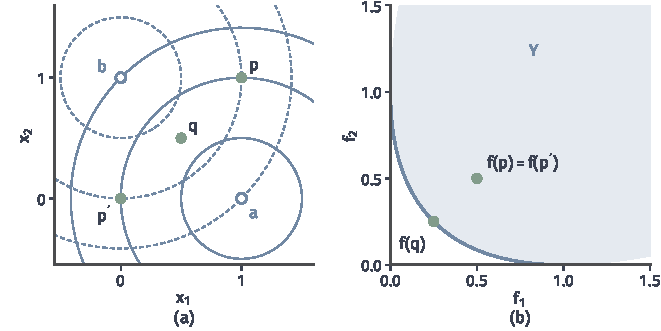
\includegraphics[width=112mm]{figures/05-optimization/07-multiple-criteria-and-nested-optimization/matplotlib/moo-two-spaces/figure.pdf}
  \caption{式~\eqref{eq:moo-iso}的决策空间与目标空间。(a)实线圆是$f_1$的等高线，虚线圆是$f_2$的等高线，绿点是三个方案。(b)浅蓝区域是可达目标集$\bm{Y}$，蓝线是它的左下边界。$\bm{p}$与$\bm{p}'$对称，映到同一个目标向量；$\bm{q}=(1/2,1/2)$的目标向量是$(1/4,1/4)$，两个分量都更小。}
  \label{fig:moo-two-spaces}
\end{BookInlineFigure}

\paragraph{为什么没有唯一的最小}
单目标问题中，任意两个实数都能比较大小，所以最小值的定义不会有歧义。向量没有这样的全序。$A=(1,8)$与$D=(6,1)$相比，成本是$A$小，误差是$D$小。两个分量的优劣方向相反，要断定谁更好，必须先说清一万元相当于多少个百分点的误差，而题目没有给出这个信息。

因此不能指望从式~\eqref{eq:moo-problem}直接得到一个点。接下来只保留不需要换算就能下的判断。

\subsection{支配关系}
\label{sec:moo-dominance}

不引入任何偏好，还能确定哪些比较？回到式~\eqref{eq:moo-candidates}，$B=(2,5)$与$E=(5,6)$相比，$B$更便宜，误差也更小。无论决策者多看重成本或多看重误差，只要两项都是越小越好，就没有理由选$E$。把这种“全面不差”写成定义。

\begin{definition}[支配]
\label{def:moo-dominance}
设$\bm{u},\bm{v}\in\bm{C}$。若
\begin{equation}
 f_i(\bm{u})\leq f_i(\bm{v})\quad\text{对所有}\ i=1,\ldots,m,
 \label{eq:moo-dom-weak}
\end{equation}
并且至少有一个$i$使$f_i(\bm{u})<f_i(\bm{v})$，就说$\bm{u}$\term{支配}（dominate）$\bm{v}$。
\end{definition}

式~\eqref{eq:moo-dom-weak}说的是“每一项都不差”，后半句说的是“至少有一项确实更好”。后半句不能省：没有它，两个目标向量相同的方案就会互相支配，而它们之间其实没有优劣。

\paragraph{用左下区域检查}
在目标平面上，支配关系可以一眼看出。以一点$\bm{y}$为角画出它的左下方区域和右上方区域，落在左下方的点支配$\bm{y}$，落在右上方的点被$\bm{y}$支配。图~\ref{fig:moo-dominance}(a)以$B$为例，平面被两条虚线分成四块。左上和右下两块中的点一个分量比$B$小，另一个分量比$B$大，这两块就是\textbf{不可比}的区域。

\begin{BookInlineFigure}
  \centering
  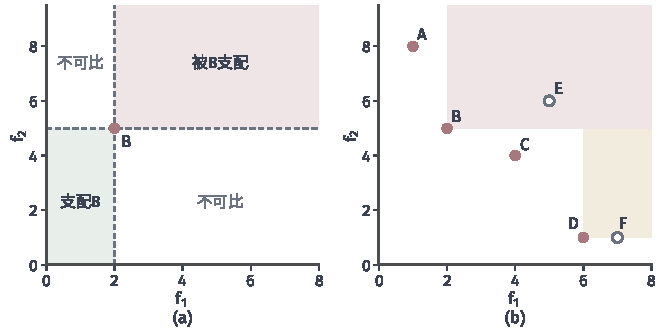
\includegraphics[width=112mm]{figures/05-optimization/07-multiple-criteria-and-nested-optimization/matplotlib/moo-dominance/figure.pdf}
  \caption{目标平面上的支配关系，数据为式~\eqref{eq:moo-candidates}。(a)以$B$为角分出的四块区域。(b)红点是不被任何候选支配的方案，空心点是被支配的方案。粉色是被$B$支配的区域，$E$在其中；浅黄是被$D$支配的区域，$F$在它的下边界上。}
  \label{fig:moo-dominance}
\end{BookInlineFigure}

下面逐对检查图~\ref{fig:moo-dominance}(b)中的六个点。$E=(5,6)$被$B$支配，也被$C=(4,4)$支配。$F=(7,1)$与$D=(6,1)$误差相同，$D$更便宜，所以$D$支配$F$。其余的$A,B,C,D$按成本从小到大排，误差依次是$8,5,4,1$，严格下降，任何两个都是一项更好、一项更差，互不支配。

支配是一种偏序：一个点不支配自己，支配关系可以传递，但并非任何两点都可比。可比的部分是确定的判断，不可比的部分要等偏好来决定。

\subsection{Pareto最优}
\label{sec:moo-pareto}

既然只有部分方案之间能比较，“最优”就只能退一步定义：没有被其他方案全面超过。这一小节给出这个定义及其两种变形，并把它们落到两个例子上。

\begin{definition}[Pareto最优]
\label{def:moo-pareto}
设$\bar{\bm{x}}\in\bm{C}$。
\begin{enumerate}
 \item 若不存在$\bm{x}\in\bm{C}$支配$\bar{\bm{x}}$，称$\bar{\bm{x}}$为\term{Pareto最优}（Pareto optimal）点。
 \item 若不存在$\bm{x}\in\bm{C}$使$f_i(\bm{x})<f_i(\bar{\bm{x}})$对所有$i$成立，称$\bar{\bm{x}}$为\term{弱Pareto最优}（weakly Pareto optimal）点。
 \item 若存在$r>0$，使上述条件在$\bm{C}$与$\bar{\bm{x}}$的$r$邻域的交集上成立，相应地称为\term{局部Pareto最优}（locally Pareto optimal）点或局部弱Pareto最优点。
\end{enumerate}
全体Pareto最优点组成的集合称为\term{Pareto解集}（Pareto set），记为$\bm{X}_{\mathrm{P}}$；它在$\bm{f}$下的像$\bm{Y}_{\mathrm{P}}=\bm{f}(\bm{X}_{\mathrm{P}})$称为\term{Pareto前沿}（Pareto front）。
\end{definition}

解集在决策空间，前沿在目标空间，二者不是同一个东西。多个方案可以对应前沿上的同一点，所以由前沿反推方案时还要保留决策变量。

未加“局部”二字的Pareto最优指全局版本，比较对象是全部可行点。全局Pareto最优点必定是局部Pareto最优点，因为比较的范围缩小了。Pareto最优点必定是弱Pareto最优点，因为所有分量都严格更小的点一定支配它。

\paragraph{有限例}
在式~\eqref{eq:moo-candidates}中，$A,B,C,D$都不被支配，都是Pareto最优点。$E$被$B$支配，且$B$的两个分量都严格小于$E$，所以$E$连弱Pareto最优点也不是。

$F=(7,1)$被$D$支配，因此不是Pareto最优点。可是要两个分量都严格小于$F$，误差必须小于$1$，而六个方案中没有这样的。所以$F$是弱Pareto最优点。弱Pareto最优这个说法宽松，正是因为它放过了“一项持平、另一项更差”的方案。

\paragraph{弱Pareto点在目标平面上的样子}
图~\ref{fig:moo-weak-pareto}中可达集合的边界有三段。红色曲线段上的点都是Pareto最优的。左侧的竖直边上，$\bm{y}$的左下方开象限（绿色）里没有可达点，所以$\bm{y}$是弱Pareto最优的；但沿着竖直边往下走到$\bm{y}'$，成本不变而误差变小，$\bm{y}'$支配$\bm{y}$。底部的水平边同理，$\bm{z}'$支配$\bm{z}$。

\begin{BookInlineFigure}
  \centering
  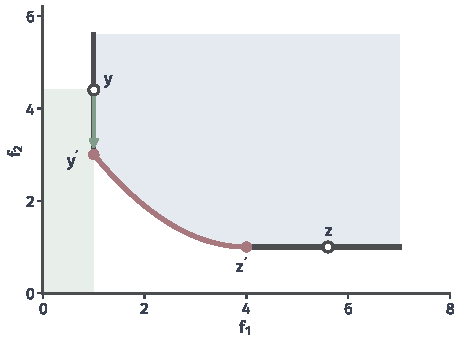
\includegraphics[width=78mm]{figures/05-optimization/07-multiple-criteria-and-nested-optimization/matplotlib/moo-weak-pareto/figure.pdf}
  \caption{弱Pareto最优点的位置。浅蓝区域是可达目标集，红色曲线是Pareto前沿，深灰粗线是只有弱Pareto性质的竖直边和水平边。绿色是$\bm{y}$的左下方开象限，其中没有可达点。绿色箭头指向支配$\bm{y}$的点$\bm{y}'$。}
  \label{fig:moo-weak-pareto}
\end{BookInlineFigure}

\paragraph{连续例：解集是一条线段}
现在求式~\eqref{eq:moo-iso}的Pareto解集。选坐标把几何关系拆开：把点写成沿$\bm{a}\to\bm{b}$的位置$s$与到连线的带符号距离$r$，
\[
 \bm{x}=\bm{a}+s(\bm{b}-\bm{a})+r\bm{e},\qquad \bm{e}=\tfrac{1}{\sqrt2}(1,1).
\]
由于$\bm{e}$是与$\bm{b}-\bm{a}$垂直的单位向量，且$\lVert\bm{b}-\bm{a}\rVert_2^2=2$，由勾股定理得到
\begin{equation}
 f_1=s^2+\tfrac12r^2,\qquad f_2=(1-s)^2+\tfrac12r^2.
 \label{eq:moo-iso-coords}
\end{equation}

式~\eqref{eq:moo-iso-coords}说明，三种情形下都能找到严格更好的点。若$r\neq0$，把$r$改为$0$，两个目标都严格减小。若$r=0$而$s<0$，把$s$改为$0$，$f_1$从$s^2$减为$0$，$f_2$从$(1-s)^2$减为$1$，两项都严格减小。$s>1$时对称。

所以Pareto最优点只可能在线段$s\in[0,1]$，$r=0$上。还要确认线段上的点确实不被支配。设$\bm{y}$支配线段上参数为$s$的点，按上面的做法把$\bm{y}$拉回线段得到参数$s'$，目标不增，于是$\bm{f}$在$s'$处的值逐项不大于在$s$处的值。

线段上$f_1=s^2$严格递增，$f_2=(1-s)^2$严格递减，两项同时不大于只能发生在$s'=s$。这样拉回前后目标向量相等，$\bm{y}$与原点目标相同，与“支配”矛盾。于是
\begin{equation}
 \bm{X}_{\mathrm{P}}=\{(1-s,s):0\leq s\leq1\},\qquad
 \bm{Y}_{\mathrm{P}}=\{(s^2,(1-s)^2):0\leq s\leq1\}.
 \label{eq:moo-iso-front}
\end{equation}

图~\ref{fig:moo-pareto-set-front}画出这一结果。线段外的点$\bm{p}=(1,1)$对应目标向量$(1/2,1/2)$，沿箭头移到$\bm{q}$后目标变成$(1/4,1/4)$，两项都减半。线段内部沿着线段移动，则是拿$f_1$换$f_2$，这种交换就是\term{取舍}（trade-off）的含义。

\begin{BookInlineFigure}
  \centering
  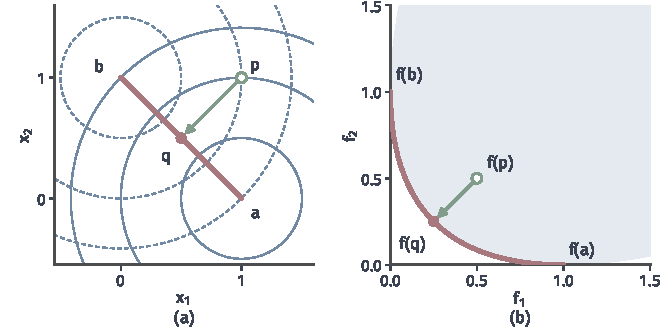
\includegraphics[width=112mm]{figures/05-optimization/07-multiple-criteria-and-nested-optimization/matplotlib/moo-pareto-set-front/figure.pdf}
  \caption{式~\eqref{eq:moo-iso}的Pareto解集与Pareto前沿。(a)决策平面上红色线段是解集，绿色箭头把线段外的点$\bm{p}$移到$\bm{q}$。(b)目标平面上浅蓝区域是可达目标集，红色曲线是前沿$(s^2,(1-s)^2)$；同一步移动使$\bm{f}(\bm{p})$沿箭头落到前沿上的$\bm{f}(\bm{q})$。}
  \label{fig:moo-pareto-set-front}
\end{BookInlineFigure}

\paragraph{局部版本与存在性}
局部Pareto最优只和附近的方案比。取一个变量$x\in[0,4]$，令
\begin{equation}
 f_1(x)=x,\qquad f_2(x)=(x-1)^2(x-3)^2+0.4x.
 \label{eq:moo-local}
\end{equation}
由于$f_1$随$x$增大，$x$越大的方案越贵，所以一个方案不被支配，要求所有更便宜的方案的误差都更大。

图~\ref{fig:moo-local-pareto}是这条曲线。$f_2$的第一个极小点约在$x\approx0.953$，记对应点为$\bm{P}$，$[0,0.953]$上的$f_2$严格下降，这一段是全局Pareto最优的（红色）。第二个极小点约在$x\approx2.946$，记对应点为$\bm{Q}$，通往$\bm{Q}$的紫色下降段上，近处更便宜的方案误差更大，近处更贵的方案误差更小，互不支配，所以这一段局部Pareto最优。

但$\bm{Q}$的两个分量约为$(2.946,1.189)$，$\bm{P}$的两个分量约为$(0.953,0.390)$，都更小，$\bm{P}$支配$\bm{Q}$。这和单目标问题中局部最小点与全局最小点的差别是一回事，只是这里比较的是向量。

\begin{BookInlineFigure}
  \centering
  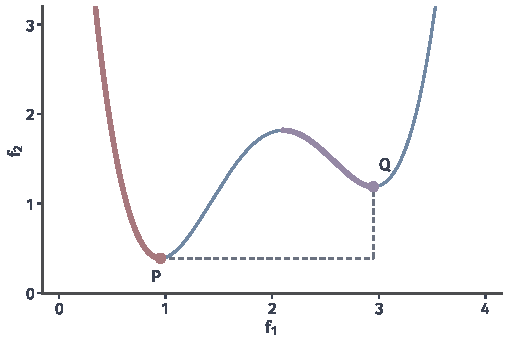
\includegraphics[width=86mm]{figures/05-optimization/07-multiple-criteria-and-nested-optimization/matplotlib/moo-local-pareto/figure.pdf}
  \caption{式~\eqref{eq:moo-local}在目标平面上的曲线。红色段全局Pareto最优，紫色段只局部Pareto最优，蓝色段的点在近处已被支配。虚线标出$\bm{P}$支配$\bm{Q}$的两个分量差。}
  \label{fig:moo-local-pareto}
\end{BookInlineFigure}

Pareto最优点也不是总存在的。取$\bm{C}=(0,1]$，$f_1(x)=f_2(x)=x$，任意$x$都被$x/2$支配，解集是空集。这和单目标问题中最小点不存在是同一种情形，第~\ref{sec:moo-scalarization}节会给出一个保证存在的条件。

\subsection{目标尺度}
\label{sec:moo-scale}

单位是人为选定的。把成本从万元换成千元，数字扩大十倍，这时哪些结论不变，哪些结论会变？

\paragraph{支配关系不受影响}
若把每个目标换成$\varphi_i(f_i)$，其中$\varphi_i$严格递增，那么$f_i(\bm{u})\leq f_i(\bm{v})$与$\varphi_i(f_i(\bm{u}))\leq\varphi_i(f_i(\bm{v}))$等价，严格不等号也一样。所以支配关系、Pareto解集、弱Pareto解集都不变。换单位是$\varphi_i(y)=cy$，$c>0$，自然在其中。

\paragraph{固定权重的加权目标会变}
把两个目标按固定权重相加，比如权重取$(0.6,0.4)$，得到一个分数，分数最低的方案胜出。以万元为单位，四个Pareto方案的分数是
\[
 A:\ 3.8,\qquad B:\ 3.2,\qquad C:\ 4,\qquad D:\ 4,
\]
所以选$B$。把成本改用千元表示，$f_1$乘以$10$，权重不变，分数变成
\[
 A:\ 9.2,\qquad B:\ 14,\qquad C:\ 25.6,\qquad D:\ 36.4,
\]
这回选$A$。方案本身什么也没变，变的只是记账单位，见图~\ref{fig:moo-scale-weight}。

\begin{BookInlineFigure}
  \centering
  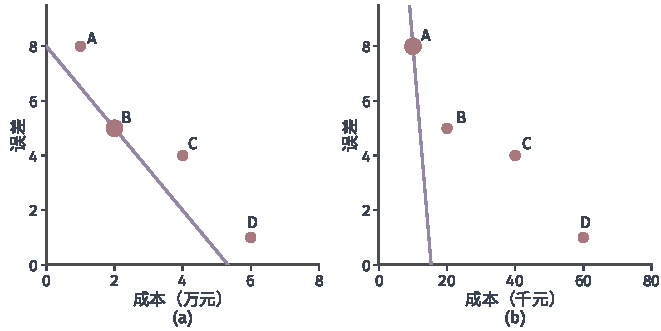
\includegraphics[width=112mm]{figures/05-optimization/07-multiple-criteria-and-nested-optimization/matplotlib/moo-scale-weight/figure.pdf}
  \caption{换单位改变加权和的选择，权重固定为$(0.6,0.4)$。紫线是经过分数最低方案的等分数线，大圆点是被选中的方案。(a)成本以万元计，选中$B$。(b)成本以千元计，选中$A$。四个点的相对位置在两图中按横轴比例对应，支配关系没有变化。}
  \label{fig:moo-scale-weight}
\end{BookInlineFigure}

\paragraph{基于距离的比较也会变}
另一种常见做法是计算到\term{理想点}（ideal point）的距离。理想点的每个分量是该目标单独能达到的最小值，这里是$(1,1)$。以万元为单位，四个方案到理想点的欧氏距离约为
\[
 A:\ 7,\qquad B:\ 4.12,\qquad C:\ 4.24,\qquad D:\ 5,
\]
$B$最近。改用千元后，理想点变为$(10,1)$，距离约为
\[
 A:\ 7,\qquad B:\ 10.77,\qquad C:\ 30.15,\qquad D:\ 50,
\]
$A$最近。距离把两个分量的差放在一起平方，单位大的分量就占了主导。

\paragraph{归一化及其参考范围}
为消除单位，常把每个目标按某个参考范围线性缩放到$[0,1]$。取目标$i$的下参考值$l_i$和上参考值$u_i$，$u_i>l_i$，令
\begin{equation}
 \tilde{f}_i=\frac{f_i-l_i}{u_i-l_i}.
 \label{eq:moo-normalize}
\end{equation}
下参考值常取理想点。上参考值常取Pareto方案中各目标的最大值，这样的点称为\term{最差点}（nadir point）。

以$A,B,C,D$的范围$l=(1,1)$，$u=(6,8)$归一化，四点变成
\[
 A:\ (0,1),\quad B:\ (0.2,0.571),\quad C:\ (0.6,0.429),\quad D:\ (1,0).
\]
到原点的距离依次约为$1$，$0.605$，$0.737$，$1$，选$B$。这一结果不再受万元或千元的影响，因为式~\eqref{eq:moo-normalize}的分子分母同时乘以同一个数。

但参考范围本身仍然影响结论。设候选集里多了一个$G=(1.5,36)$，它被$A$支配，本该无关紧要。若范围取全部候选的最大值，误差的上参考值变成$36$，四点的归一化误差都缩小，距离依次约为$0.2$，$0.230$，$0.606$，$1$，选中的方案从$B$变成$A$，见图~\ref{fig:moo-scale-range}。

\begin{BookInlineFigure}
  \centering
  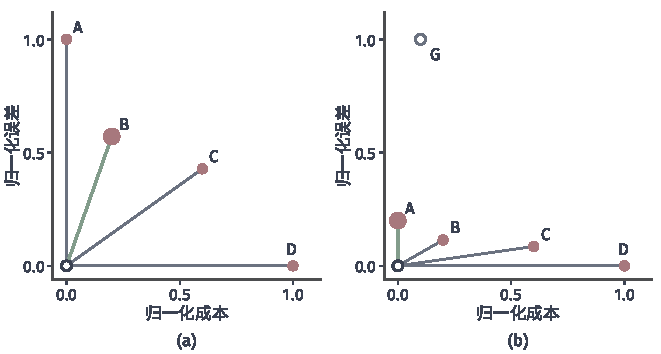
\includegraphics[width=112mm]{figures/05-optimization/07-multiple-criteria-and-nested-optimization/matplotlib/moo-scale-range/figure.pdf}
  \caption{参考范围对归一化比较的影响。线段是各方案到理想点（原点）的距离，绿色线段是最短的一条，大圆点是被选中的方案。(a)以$A,B,C,D$的范围归一化，选$B$。(b)候选中混入被支配的$G=(1.5,36)$，误差范围变大，选$A$。}
  \label{fig:moo-scale-range}
\end{BookInlineFigure}

这里的教训有两条。凡是用到权重或距离的比较，都要写明所用的单位或参考范围。归一化不是中性的操作，它把“一单位误差值多少钱”换成了“各目标范围的一格彼此相当”，这也是一种偏好，只是不那么显眼。参考范围最好由被信任的方案决定，并在结果中报告，不让被支配的候选参与定尺度。

\section{标量化}
\label{sec:moo-scalarization}

决策者往往能说出某种偏好：一项指标值多少钱，或者预算不能超过多少，或者希望各项都接近某个水平。有了偏好，就可以把多目标问题改写成单目标问题，再调用前面各章的方法。这样的改写称为\term{标量化}（scalarization）。

每种改写的解是不是Pareto最优点？改写的参数变化时，能到达前沿上的哪些点？要记住的一点是，标量化问题的解只代表这一次写下的偏好，不是“多目标问题的解”。

\subsection{加权和}
\label{sec:moo-weighted}

最直接的偏好是价格：给每个目标定一个单价，只看总价。这一小节研究按总价选出的方案有什么性质，以及扫遍所有价格能不能走遍前沿。

\paragraph{定义与直观}
取权重$\bm{w}$属于单纯形
\[
 \Delta_m=\Bigl\{\bm{w}\in\mathbb{R}^m:w_i\geq0,\ \sum_{i=1}^mw_i=1\Bigr\},
\]
求解
\begin{equation}
 \min_{\bm{x}\in\bm{C}}\ \sum_{i=1}^mw_if_i(\bm{x}).
 \label{eq:moo-weighted}
\end{equation}
这种做法称为\term{加权和法}（weighted-sum method）。两个目标时，把权重简写成$\bm{w}=(w,1-w)$，$w\in[0,1]$。

在目标平面上，总价相同的点组成一条法向为$\bm{w}$的直线。最小化总价，就是让这条直线从左下方平移过来，直到第一次碰到可达目标集。碰到的点就是解，这条直线称为\term{支撑线}（supporting line）。下面的讨论几乎都从这幅图景得来，见图~\ref{fig:moo-weighted-support}。

\begin{BookInlineFigure}
  \centering
  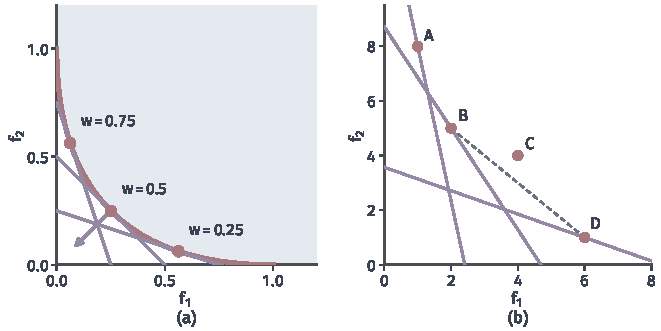
\includegraphics[width=112mm]{figures/05-optimization/07-multiple-criteria-and-nested-optimization/matplotlib/moo-weighted-support/figure.pdf}
  \caption{加权和的支撑线，紫线是最低的等总价线。(a)式~\eqref{eq:moo-iso}的前沿（红色），$w=0.25,0.5,0.75$时的切点；紫色箭头是$w=0.5$时的负法向，指向总价下降的方向。(b)式~\eqref{eq:moo-candidates}中$A,B,C,D$四点，$w=0.3,0.65,0.85$的支撑线分别经过$D,B,A$；$C$在虚线$BD$上方，任何支撑线都先碰到别的点。}
  \label{fig:moo-weighted-support}
\end{BookInlineFigure}

\paragraph{加权和的解与Pareto最优}
解的性质由权重的符号决定。权重全正时，支配者在总价上一定严格更便宜，所以解不会被支配。权重有零时，零权重目标的严格改善不计入总价，只能得到较弱的结论。

\begin{theorem}[加权和的解]
\label{thm:moo-weighted}
设$\bm{x}^\star$是问题~\eqref{eq:moo-weighted}的全局最优解。
\begin{enumerate}
 \item 若所有$w_i>0$，则$\bm{x}^\star$是Pareto最优点。
 \item 若$\bm{w}\in\Delta_m$，则$\bm{x}^\star$是弱Pareto最优点。
 \item 若$\bm{w}\in\Delta_m$，且$\bm{x}^\star$是问题~\eqref{eq:moo-weighted}的唯一全局最优解，则$\bm{x}^\star$是Pareto最优点。
\end{enumerate}
\end{theorem}

\begin{proof}
记$\phi(\bm{x})=\sum_iw_if_i(\bm{x})$。

(1)若$\bm{u}\in\bm{C}$支配$\bm{x}^\star$，则$w_if_i(\bm{u})\leq w_if_i(\bm{x}^\star)$对所有$i$成立。对$f_i(\bm{u})<f_i(\bm{x}^\star)$的那个$i$，由$w_i>0$得严格不等号。逐项相加得$\phi(\bm{u})<\phi(\bm{x}^\star)$，矛盾。

(2)若$\bm{u}\in\bm{C}$使$f_i(\bm{u})<f_i(\bm{x}^\star)$对所有$i$成立，由于$\bm{w}\in\Delta_m$，至少有一个$w_i>0$，相加仍得$\phi(\bm{u})<\phi(\bm{x}^\star)$，矛盾。

(3)若$\bm{u}\in\bm{C}$支配$\bm{x}^\star$，由$w_i\geq0$得$\phi(\bm{u})\leq\phi(\bm{x}^\star)$，所以$\bm{u}$也是全局最优解。由唯一性$\bm{u}=\bm{x}^\star$，这与“至少一项严格更小”矛盾。
\end{proof}

三条结论都只用到全局最优性，没有用到凸性。定理的第~1条马上回答了第~\ref{sec:moo-pareto}节留下的存在性问题。

\begin{theorem}[Pareto最优点的存在]
\label{thm:moo-existence}
设$\bm{C}$非空紧，各$f_i$在$\bm{C}$上连续，则Pareto解集非空。
\end{theorem}

\begin{proof}
取$w_i=1/m$。连续函数$\sum_iw_if_i$在非空紧集上取得最小值，这是第~\ref{chap:optimization}章的结论。由定理~\ref{thm:moo-weighted}的第~1条，最小点是Pareto最优点。
\end{proof}

第~\ref{sec:moo-pareto}节的反例中$\bm{C}=(0,1]$不闭，紧性不成立。

\paragraph{连续例：权重到前沿的对应}
对例~\eqref{eq:moo-iso}，由式~\eqref{eq:moo-iso-coords}，总价是
\[
 w\,s^2+(1-w)(1-s)^2+\tfrac12r^2.
\]
先取$r=0$，再对$s$求导令其为零：
\[
 2ws-2(1-w)(1-s)=0.
\]
解得$s=1-w$，也就是$\bm{x}=(w,1-w)$，对应前沿上的点
\begin{equation}
 \bigl(f_1,f_2\bigr)=\bigl((1-w)^2,\ w^2\bigr).
 \label{eq:moo-iso-weighted}
\end{equation}

前沿在该点的斜率也能算出来。由式~\eqref{eq:moo-iso-front}，$\mathrm{d}f_2/\mathrm{d}f_1=-(1-s)/s=-w/(1-w)$，正好等于等总价线的斜率。价格比决定了切点的位置，这就是图~\ref{fig:moo-weighted-support}(a)显示的情况。

例如$w=1/2$时，解是$\bm{x}=(1/2,1/2)$，目标是$(1/4,1/4)$。端点$\bm{x}=\bm{a}$只有在$w=1$时才能得到，此时权重有零，但解唯一，由定理~\ref{thm:moo-weighted}的第~3条它仍是Pareto最优点。

\paragraph{有限例：下包络}
对式~\eqref{eq:moo-candidates}，每个候选的总价是$w$的一次函数：
\[
 \begin{gathered}
  A:\ 8-7w,\quad B:\ 5-3w,\quad C:\ 4,\\
  D:\ 1+5w,\quad E:\ 6-w,\quad F:\ 1+6w.
 \end{gathered}
\]
图~\ref{fig:moo-weighted-envelope}把六条直线画在一起，每个$w$上的最小值组成红色的下包络。$w<1/2$时$D$最便宜，$1/2<w<3/4$时$B$最便宜，$w>3/4$时$A$最便宜。

\begin{BookInlineFigure}
  \centering
  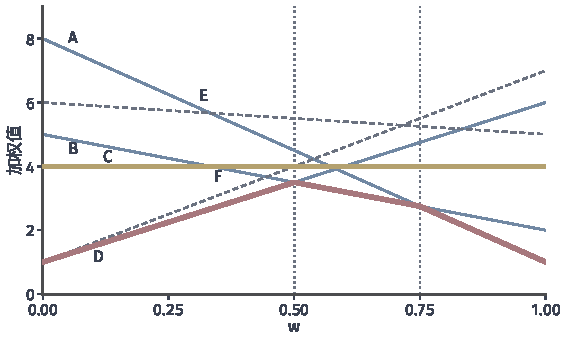
\includegraphics[width=96mm]{figures/05-optimization/07-multiple-criteria-and-nested-optimization/matplotlib/moo-weighted-envelope/figure.pdf}
  \caption{六个候选的总价随权重$w$的变化。红线是下包络，其转折点在$w=1/2$和$w=3/4$。黄线是$C$，它始终在下包络之上。虚线是被支配的$E$和$F$。}
  \label{fig:moo-weighted-envelope}
\end{BookInlineFigure}

$C$虽然是Pareto最优点，却永远选不上。要比$B$便宜，需要$4\leq5-3w$，即$w\leq1/3$；要比$D$便宜，需要$4\leq1+5w$，即$w\geq3/5$。两个要求不能同时满足。

几何上，线段$BD$在$f_1=4$处的高度是$3$，而$C$的高度是$4$，$C$位于线段上方。能被某组权重选中的Pareto点称为\term{支撑点}（supported point），$C$不是支撑点。

下包络也说明了解的跳变：$w$从小到大扫过$1/2$时，答案从$D$直接跳到$B$，两者的总价都是$3.5$；扫过$3/4$时从$B$跳到$A$，总价都是$2.75$。

零权重的情形也可以在这里看到。$w=0$时总价就是误差，$D$和$F$都等于$1$，并列最优，而$F$被$D$支配。定理~\ref{thm:moo-weighted}只保证$F$是弱Pareto最优点，这个结论不能再加强。

\paragraph{凸问题：非负权重足够覆盖}
前面的例子表明，非凸时支撑点可能不是全部。凸性保证的是，不存在$C$那样藏在凹陷里的点。

\begin{theorem}[凸问题的支撑权重]
\label{thm:moo-convex-support}
设$\bm{C}$凸，各$f_i$在$\bm{C}$上凸。若$\bar{\bm{x}}$是全局弱Pareto最优点，则存在$\bm{w}\in\Delta_m$，使$\bar{\bm{x}}$是问题~\eqref{eq:moo-weighted}的全局最优解。
\end{theorem}

证明的思路是把可达集合向右上方“加厚”，使它成为凸集，再用超平面把它与$\bar{\bm{y}}$左下方的点隔开。所用的严格分离定理在第~\ref{chap:duality}章已经证明：一点若不在闭凸集中，就存在超平面把二者严格分开。

\begin{proof}
记$\bar{\bm{y}}=\bm{f}(\bar{\bm{x}})$，记全$1$向量为$\bm{1}$。令
\[
 \bm{A}=\{\bm{f}(\bm{x})+\bm{t}:\bm{x}\in\bm{C},\ \bm{t}\geq\bm{0}\}.
\]

先说明$\bm{A}$凸。取$\bm{f}(\bm{x})+\bm{t}$与$\bm{f}(\bm{x}')+\bm{t}'$，$\gamma\in[0,1]$。由$f_i$凸，
\[
 \bm{f}(\gamma\bm{x}+(1-\gamma)\bm{x}')\leq\gamma\bm{f}(\bm{x})+(1-\gamma)\bm{f}(\bm{x}'),
\]
差额并入$\bm{t}$的凸组合，所以这两点的凸组合仍在$\bm{A}$中。于是闭包$\operatorname{cl}\bm{A}$是闭凸集。

对$\epsilon>0$，点$\bm{z}_\epsilon=\bar{\bm{y}}-\epsilon\bm{1}$不在$\operatorname{cl}\bm{A}$中。否则有$\bm{A}$中的点列趋于$\bm{z}_\epsilon$，其中某一点的每个分量都严格小于$\bar{\bm{y}}$的相应分量。这个点形如$\bm{f}(\bm{x})+\bm{t}$，于是$f_i(\bm{x})<\bar{y}_i$对所有$i$成立，与弱Pareto最优矛盾。

由严格分离定理，取单位向量$\bm{c}_\epsilon$，使对所有$\bm{x}\in\bm{C}$，$\bm{t}\geq\bm{0}$，
\[
 \langle\bm{c}_\epsilon,\bm{f}(\bm{x})+\bm{t}\rangle>\langle\bm{c}_\epsilon,\bm{z}_\epsilon\rangle.
\]
若$\bm{c}_\epsilon$有负分量，让$\bm{t}$的相应分量趋于无穷，左端趋于$-\infty$，矛盾，所以$\bm{c}_\epsilon\geq\bm{0}$。

单位球面紧，取$\epsilon\downarrow0$的子列使$\bm{c}_\epsilon\to\bm{c}$。则$\bm{c}\geq\bm{0}$，$\bm{c}\neq\bm{0}$。在上式中取$\bm{t}=\bm{0}$，令$\epsilon\downarrow0$，得到
\[
 \langle\bm{c},\bm{f}(\bm{x})\rangle\geq\langle\bm{c},\bar{\bm{y}}\rangle\quad\text{对所有}\ \bm{x}\in\bm{C}.
\]
令$\bm{w}=\bm{c}/\sum_ic_i\in\Delta_m$，上式就是$\bar{\bm{x}}$最小化$\sum_iw_if_i$。
\end{proof}

定理的结论是“存在非负权重”，不是“存在全正权重”。例~\eqref{eq:moo-iso}的端点$\bm{a}$只有权重$(1,0)$能选中，就说明全正的要求一般做不到。定理的条件也不能去掉，图~\ref{fig:moo-weighted-nonconvex}的两个例子都不满足凸性。

\paragraph{非凸前沿上的遗漏}
第三个例子是一个一元问题：$x\in[0,1]$，
\begin{equation}
 f_1(x)=x,\qquad f_2(x)=1-x^2.
 \label{eq:moo-concave}
\end{equation}
$f_1$递增，$f_2$递减，所以每个$x$都是Pareto最优点，前沿是向右上方鼓起的抛物线。加权目标是
\[
 w\,x+(1-w)(1-x^2).
\]
它是$x$的凹函数，在区间上的最小值只能在端点取到，分别是$x=0$时的$1-w$和$x=1$时的$w$。

于是$w>1/2$时解是$x=0$，$w<1/2$时解是$x=1$，$w=1/2$时两端并列。无论权重取什么，中间的方案都选不到。图~\ref{fig:moo-weighted-nonconvex}(a)中三条紫线都只能碰到两个端点。

\begin{BookInlineFigure}
  \centering
  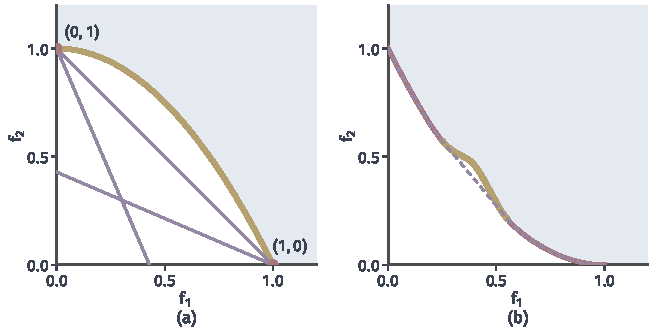
\includegraphics[width=112mm]{figures/05-optimization/07-multiple-criteria-and-nested-optimization/matplotlib/moo-weighted-nonconvex/figure.pdf}
  \caption{加权和遗漏的前沿。(a)式~\eqref{eq:moo-concave}的前沿，紫线是$w=0.3,0.5,0.7$的支撑线，都只碰到端点（红点），黄色段上的点都选不到。(b)带凹陷的前沿$f_2=(1-f_1)^2+0.1\exp(-((f_1-0.4)/0.1)^2)$，紫色虚线是它的下凸包，黄色段（$0.25<f_1<0.55$）位于凸包上方，选不到。}
  \label{fig:moo-weighted-nonconvex}
\end{BookInlineFigure}

现实中的前沿常常只有一段凹陷。图~\ref{fig:moo-weighted-nonconvex}(b)中，前沿由一个下凸的主体和一个小鼓包组成。任何方向的支撑线都不会碰到黄色段内部，紫色虚线就是它的\term{下凸包}（lower convex hull），凹陷中的点都比这条线高。从图上也可以知道，权重一旦扫过黄色段两端所对应的斜率，答案就从一端跳到另一端。

所以，“扫描权重”只能得到支撑点。对非凸问题，这可能漏掉前沿的大部分。

\subsection{阈值约束}
\label{sec:moo-threshold}

很多需求本来就不是价格，而是硬指标：预算不超过某个数，在此前提下误差尽量小。这一小节把这种需求写成约束，研究它和加权和有什么不同。

\paragraph{定义}
保留第$j$个目标作为被最小化的量，其余目标用阈值$\tau_i$限制：
\begin{equation}
 \min_{\bm{x}\in\bm{C}}\ f_j(\bm{x})
 \quad\text{s.t.}\quad f_i(\bm{x})\leq\tau_i,\ \ i\neq j.
 \label{eq:moo-threshold}
\end{equation}
这种做法称为\term{阈值约束法}（$\varepsilon$-constraint method）。这是一个普通的约束优化问题，第~\ref{chap:constrained-optimality}章的最优性条件和前一部分各章的求解方法都能直接用上。

在目标平面上，两个目标时阈值约束是一条竖线$f_1\leq\tau$，竖线左侧的部分是可行的，问题就是在其中找最低点。这条竖线不需要从外部支撑可达集合，所以能插进前沿的凹陷里。

\paragraph{解的性质}
和加权和不同，这里的结论有反方向的一半，而且不需要凸性。

\begin{theorem}[阈值约束的解]
\label{thm:moo-threshold}
固定$j$与阈值$\tau_i$，$i\neq j$。
\begin{enumerate}
 \item 问题~\eqref{eq:moo-threshold}的每个全局最优解都是弱Pareto最优点；若全局最优解唯一，它是Pareto最优点。
 \item 若$\bar{\bm{x}}$是Pareto最优点，取$\tau_i=f_i(\bar{\bm{x}})$，$i\neq j$，则$\bar{\bm{x}}$是问题~\eqref{eq:moo-threshold}的全局最优解。
 \item 设$\bm{S}$是问题~\eqref{eq:moo-threshold}的全局最优解集。若$\tilde{\bm{x}}$在$\bm{S}$上最小化$\sum_{i\neq j}f_i$，则$\tilde{\bm{x}}$是Pareto最优点。
\end{enumerate}
\end{theorem}

\begin{proof}
(1)设$\hat{\bm{x}}$是全局最优解。若$\bm{u}\in\bm{C}$的各目标都严格小于$\hat{\bm{x}}$，则$f_i(\bm{u})<f_i(\hat{\bm{x}})\leq\tau_i$，$\bm{u}$可行，而$f_j(\bm{u})<f_j(\hat{\bm{x}})$，矛盾。

若$\hat{\bm{x}}$是唯一全局最优解，设$\bm{u}$支配$\hat{\bm{x}}$。同样$\bm{u}$可行，且$f_j(\bm{u})\leq f_j(\hat{\bm{x}})$，所以$\bm{u}$也是全局最优解。由唯一性$\bm{u}=\hat{\bm{x}}$，与支配矛盾。

(2)$\bar{\bm{x}}$满足$f_i(\bar{\bm{x}})\leq\tau_i$，可行。若可行点$\bm{u}$使$f_j(\bm{u})<f_j(\bar{\bm{x}})$，再由可行性$f_i(\bm{u})\leq\tau_i=f_i(\bar{\bm{x}})$，$\bm{u}$支配$\bar{\bm{x}}$，矛盾。

(3)设$\bm{u}\in\bm{C}$支配$\tilde{\bm{x}}$。各约束下$f_i(\bm{u})\leq f_i(\tilde{\bm{x}})\leq\tau_i$，$\bm{u}$可行；又$f_j(\bm{u})\leq f_j(\tilde{\bm{x}})$，所以$\bm{u}\in\bm{S}$，且$f_j(\bm{u})=f_j(\tilde{\bm{x}})$。于是严格减小的分量在$i\neq j$中，$\sum_{i\neq j}f_i(\bm{u})<\sum_{i\neq j}f_i(\tilde{\bm{x}})$，矛盾。
\end{proof}

第~2条说的是，每个Pareto点都能被某组阈值选中，即使它不是支撑点。第~3条给出处理并列最优解的办法：先满足阈值并最小化$f_j$，再在并列的解中比较其余目标。这种分步择优也叫字典序的处理。

\paragraph{有限例与不可行}
在式~\eqref{eq:moo-candidates}上取$j=2$，以成本为预算$\tau$，求误差的最小值
\begin{equation}
 v(\tau)=\min\{f_2:f_1\leq\tau\}.
 \label{eq:moo-threshold-value}
\end{equation}
逐段比较得到：
\[
 v(\tau)=
 \begin{cases}
  \text{不可行},&\tau<1,\\
  8\ (A),&1\leq\tau<2,\\
  5\ (B),&2\leq\tau<4,\\
  4\ (C),&4\leq\tau<6,\\
  1\ (D),&\tau\geq6.
 \end{cases}
\]

这张表说明了三件事。阈值过紧时问题不可行，应当如实报告“不存在满足要求的方案”，不要输出一个违反约束的点。预算扫过$4$时选中了$C$，这个点加权和永远选不到。$\tau\geq7$时$D$与$F$并列，而$F$被$D$支配，这时按定理~\ref{thm:moo-threshold}的第~3条再比较成本，就排除了$F$。

\begin{BookInlineFigure}
  \centering
  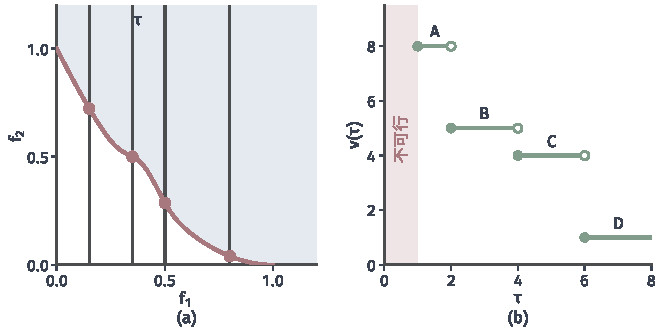
\includegraphics[width=112mm]{figures/05-optimization/07-multiple-criteria-and-nested-optimization/matplotlib/moo-threshold-scan/figure.pdf}
  \caption{阈值约束的扫描。(a)图~\ref{fig:moo-weighted-nonconvex}(b)的前沿，深灰竖线是四个阈值，红点是相应的解，其中两个点在加权和选不到的凹陷段内。(b)有限例的$v(\tau)$，实心点属于该段，空心点不属于；粉色区域不可行，字母是选中的方案。}
  \label{fig:moo-threshold-scan}
\end{BookInlineFigure}

图~\ref{fig:moo-threshold-scan}(a)显示，阈值从左向右扫过时，解沿整条前沿移动。代价是每次都要解一个带约束的问题，这比加权和难：加权和只是一个无约束问题，这里多了一个可能起作用的约束。

\paragraph{阈值与价格的联系}
阈值$\tau$和价格$w$看起来是两种语言，通过乘子可以把它们联系起来。把例~\eqref{eq:moo-iso}写成$j=2$的阈值问题，
\[
 \min\ f_2(\bm{x})\quad\text{s.t.}\quad f_1(\bm{x})\leq\tau,
\]
约束起作用时，KKT驻定条件（第~\ref{chap:constrained-optimality}章）要求
\begin{equation}
 \nabla f_2(\bm{x})+\lambda\nabla f_1(\bm{x})=\bm{0},\qquad\lambda\geq0.
 \label{eq:moo-threshold-kkt}
\end{equation}

式~\eqref{eq:moo-threshold-kkt}除以$1+\lambda$，就是权重$\bm{w}=(\lambda,1)/(1+\lambda)$的加权和的驻定条件。乘子$\lambda$就是目标$f_1$相对于$f_2$的价格。

具体计算。在解的线段上$f_1=s^2=\tau$，所以$s=\sqrt\tau$，且$r=0$。式~\eqref{eq:moo-threshold-kkt}沿线段方向的分量给出$(s-1)+\lambda s=0$，于是
\begin{equation}
 \lambda(\tau)=\frac{1-\sqrt\tau}{\sqrt\tau},\qquad 0<\tau\leq1.
 \label{eq:moo-iso-lambda}
\end{equation}

例如$\tau=1/4$时，$s=1/2$，$\lambda=1$，权重正是$(1/2,1/2)$，解与式~\eqref{eq:moo-iso-weighted}中$w=1/2$的解相同。

式~\eqref{eq:moo-iso-lambda}也描述了$\tau$增大时价格怎样变化。由式~\eqref{eq:moo-iso-front}，最优值$v(\tau)=(1-\sqrt\tau)^2$，求导得
\[
 v'(\tau)=-\frac{1-\sqrt\tau}{\sqrt\tau}=-\lambda(\tau).
\]
放宽一单位阈值，最优值下降$\lambda$，这与第~\ref{chap:parametric-sensitivity}章乘子是影子价格的结论一致。图~\ref{fig:moo-threshold-price}画出了这一点。$\tau$接近$0$时$\lambda$趋于无穷，$\tau\geq1$时约束不再起作用，$\lambda=0$，解停在$\bm{b}$。

\begin{BookInlineFigure}
  \centering
  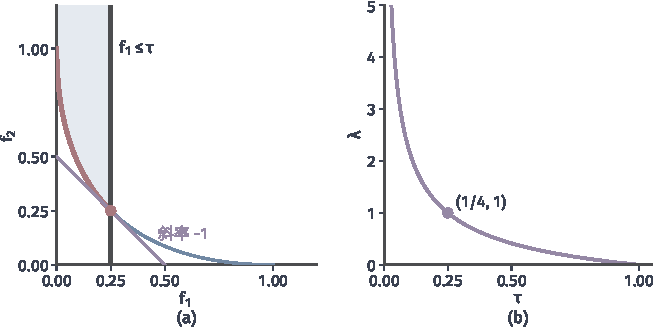
\includegraphics[width=112mm]{figures/05-optimization/07-multiple-criteria-and-nested-optimization/matplotlib/moo-threshold-price/figure.pdf}
  \caption{阈值与价格，例~\eqref{eq:moo-iso}。(a)深灰竖线是阈值$f_1\leq1/4$，可行部分为左侧浅蓝区域，红色段是可行的前沿，红点是解；紫线是前沿在该点的切线，斜率$-\lambda=-1$。(b)乘子随阈值的变化，式~\eqref{eq:moo-iso-lambda}。}
  \label{fig:moo-threshold-price}
\end{BookInlineFigure}

这种对应只在问题有相应结构时才是一一对应。非凸时，凹陷中的解仍满足式~\eqref{eq:moo-threshold-kkt}，但它只是相应加权和的驻定点，不是最小点。阈值问题的解能到达加权和到不了的地方，正是因为这里的约束替代了全局的比较。

\paragraph{并列最优解}
前沿出现水平段时，阈值问题的解不唯一。图~\ref{fig:moo-threshold-tie}中，阈值$\tau$落在底部水平边的范围内，$\bm{z}'$和$\bm{z}$的$f_2$都等于最小值，黄色线段上的点都是最优解。$\bm{z}$被$\bm{z}'$支配。

\begin{BookInlineFigure}
  \centering
  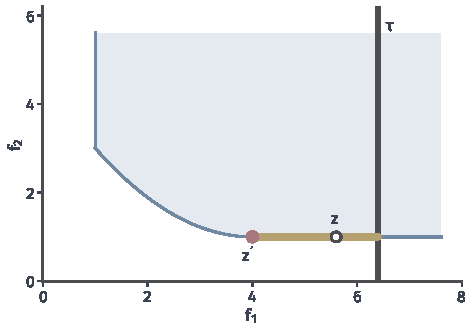
\includegraphics[width=80mm]{figures/05-optimization/07-multiple-criteria-and-nested-optimization/matplotlib/moo-threshold-tie/figure.pdf}
  \caption{阈值约束的并列最优解。深灰竖线是阈值，黄色线段是$\min\{f_2:f_1\leq\tau\}$的全部解的目标值。空心点$\bm{z}$是弱Pareto最优点，红点$\bm{z}'$是在并列解中进一步最小化$f_1$后得到的Pareto最优点。}
  \label{fig:moo-threshold-tie}
\end{BookInlineFigure}

求解器一般只返回并列解中的某一个，不一定是$\bm{z}'$。所以，只要阈值问题的解不能确认唯一，就要做第二阶段的择优，否则报告的只是一个弱Pareto最优点。

\subsection{参考点方法}
\label{sec:moo-reference}

有时决策者说的既不是价格，也不是预算，而是希望各项指标都接近某个水平。这一小节把这种需求写成到参考点的最大偏差，它能选中加权和选不到的点，又不必增加约束。

\paragraph{定义}
设各目标在$\bm{C}$上有有限下界，取\term{参考点}（reference point）$\bm{z}$，使$z_i<\inf_{\bm{C}}f_i$对所有$i$成立。再取权重$w_i>0$，最小化带权的最大偏差：
\begin{equation}
 \min_{\bm{x}\in\bm{C}}\ \max_{1\leq i\leq m}\ w_i\bigl(f_i(\bm{x})-z_i\bigr).
 \label{eq:moo-chebyshev}
\end{equation}
这种做法称为\term{加权Chebyshev标量化}（weighted Chebyshev scalarization）。

式~\eqref{eq:moo-chebyshev}的直观含义是，目标被缩放后，看离参考点最远的一项。下水平集是以$\bm{z}$为左下角的长方形，边长比由权重决定。随着水平增大，长方形的右上角沿着从$\bm{z}$出发、方向为$(1/w_1,\ldots,1/w_m)$的射线向外移动。长方形第一次碰到可达集合时的水平，就是最优值。

长方形的右上角尖尖地探出去，而加权和的直线是平的。平的直线碰不到凹陷，尖的角能探进去，见图~\ref{fig:moo-chebyshev-level}。

\begin{BookInlineFigure}
  \centering
  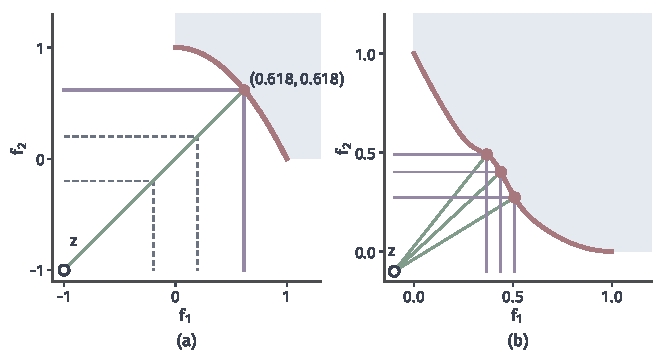
\includegraphics[width=112mm]{figures/05-optimization/07-multiple-criteria-and-nested-optimization/matplotlib/moo-chebyshev-level/figure.pdf}
  \caption{加权Chebyshev的水平集，空心点是参考点$\bm{z}$，绿线是沿$(1/w_1,1/w_2)$的射线。(a)式~\eqref{eq:moo-concave}的前沿，$\bm{z}=(-1,-1)$，$\bm{w}=(1/2,1/2)$；灰色虚线是较低水平的长方形边界，紫线是最优水平，角落碰到$(0.618,0.618)$。(b)图~\ref{fig:moo-weighted-nonconvex}(b)的前沿，$\bm{z}=(-0.1,-0.1)$，三组权重的解都在凹陷段内，紫线是相应的最优长方形边界。}
  \label{fig:moo-chebyshev-level}
\end{BookInlineFigure}

\paragraph{解的性质}
先看式~\eqref{eq:moo-chebyshev}的解是什么点，再看能选到哪些点。

\begin{theorem}[加权Chebyshev的解]
\label{thm:moo-chebyshev}
设$\bm{z}$严格低于各目标的下确界。
\begin{enumerate}
 \item 对任意$w_i>0$，问题~\eqref{eq:moo-chebyshev}的全局最优解都是弱Pareto最优点。
 \item 若$\bar{\bm{x}}$是弱Pareto最优点，取
 \begin{equation}
  w_i=\frac{1}{f_i(\bar{\bm{x}})-z_i},
  \label{eq:moo-chebyshev-weight}
 \end{equation}
 则$\bar{\bm{x}}$是问题~\eqref{eq:moo-chebyshev}的全局最优解。
 \item 设$\bm{S}$是问题~\eqref{eq:moo-chebyshev}的全局最优解集。若$\tilde{\bm{x}}$在$\bm{S}$上最小化$\sum_if_i$，则$\tilde{\bm{x}}$是Pareto最优点。
\end{enumerate}
\end{theorem}

\begin{proof}
记$\psi(\bm{x})=\max_iw_i(f_i(\bm{x})-z_i)$。

(1)设$\bm{x}^\star$是全局最优解。若$\bm{u}$的各目标都严格小于$\bm{x}^\star$，由$w_i>0$，对所有$i$有
\[
 w_i(f_i(\bm{u})-z_i)<w_i(f_i(\bm{x}^\star)-z_i)\leq\psi(\bm{x}^\star).
\]
有限个严格不等式取最大仍严格，$\psi(\bm{u})<\psi(\bm{x}^\star)$，矛盾。

(2)由$z_i<\inf f_i$，式~\eqref{eq:moo-chebyshev-weight}中分母为正，$w_i>0$，并且
\[
 w_i\bigl(f_i(\bar{\bm{x}})-z_i\bigr)=1\quad\text{对所有}\ i,
\]
所以$\psi(\bar{\bm{x}})=1$。若有$\bm{u}$使$\psi(\bm{u})<1$，则$w_i(f_i(\bm{u})-z_i)<1$对所有$i$成立，代入$w_i$的定义得$f_i(\bm{u})<f_i(\bar{\bm{x}})$对所有$i$成立，与弱Pareto最优矛盾。

(3)设$\bm{u}$支配$\tilde{\bm{x}}$。各项$f_i(\bm{u})\leq f_i(\tilde{\bm{x}})$，由$w_i>0$得$\psi(\bm{u})\leq\psi(\tilde{\bm{x}})$，所以$\bm{u}\in\bm{S}$。又有一项严格减小，$\sum_if_i(\bm{u})<\sum_if_i(\tilde{\bm{x}})$，矛盾。
\end{proof}

$\bm{z}$严格低于下确界的条件保证了第~2条的权重有限且为正。第~2条不需要凸性，这也是这种标量化比加权和强的地方：调整权重可以选中每一个弱Pareto最优点，当然也包括每一个Pareto最优点。

\paragraph{算一个连续的例子}
对式~\eqref{eq:moo-concave}取$\bm{z}=(-1,-1)$，它低于两个目标的下确界$0$。取$\bm{w}=(1/2,1/2)$，目标是
\[
 \psi(x)=\frac12\max\bigl\{x+1,\ 2-x^2\bigr\}.
\]
$x+1$递增，$2-x^2$递减，最大值的最小点在两者相等处：
\[
 x+1=2-x^2,\quad\text{即}\quad x^2+x-1=0.
\]
解得$x=(\sqrt5-1)/2\approx0.618$，目标向量也是$(0.618,0.618)$，这是加权和选不到的中间点。

\paragraph{有限例：并列最优仍会发生}
在式~\eqref{eq:moo-candidates}上取$\bm{z}=(0,0)$，它严格低于下确界$(1,1)$。取$\bm{w}=(1/2,1/2)$，各候选的$\psi$值为
\[
 A:\ 4,\quad B:\ 2.5,\quad C:\ 2,\quad D:\ 3,\quad E:\ 3,\quad F:\ 3.5.
\]
最小的是$C$，这正是加权和选不到的方案，见图~\ref{fig:moo-chebyshev-finite}(a)。

再取$\bm{w}=(0.1,0.9)$，各候选的$\psi$值为
\[
 A:\ 7.2,\quad B:\ 4.5,\quad C:\ 3.6,\quad D:\ 0.9,\quad E:\ 5.4,\quad F:\ 0.9.
\]
$D$与$F$并列最小。此时第二个目标的偏差决定了最大值，第一个目标的差别被$\max$吞掉了，$F$虽然被$D$支配，却同样最优，见图~\ref{fig:moo-chebyshev-finite}(b)。按定理~\ref{thm:moo-chebyshev}的第~3条再比较$\sum_if_i$，$D$的和是$7$，$F$的和是$8$，排除了$F$。

\begin{BookInlineFigure}
  \centering
  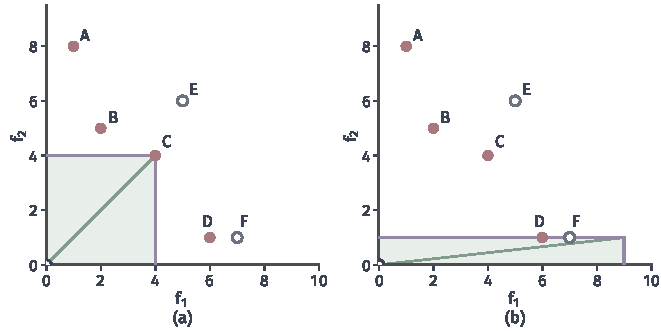
\includegraphics[width=112mm]{figures/05-optimization/07-multiple-criteria-and-nested-optimization/matplotlib/moo-chebyshev-finite/figure.pdf}
  \caption{有限候选上的加权Chebyshev，参考点$\bm{z}=(0,0)$（空心点在原点）。绿色长方形是最优水平的下水平集，紫线是其右上边界。(a)$\bm{w}=(1/2,1/2)$，长方形的角落碰到$C$。(b)$\bm{w}=(0.1,0.9)$，长方形的上边同时碰到$D$和$F$，$F$是并列的弱Pareto最优点。}
  \label{fig:moo-chebyshev-finite}
\end{BookInlineFigure}

\paragraph{三种写法的比较}
表~\ref{tab:moo-scalarization}汇总了三种标量化。没有哪一种处处占优。加权和最容易求解，但只能到达支撑点；阈值约束和加权Chebyshev能到达每个Pareto点，代价是多了约束或非光滑的$\max$。后者可以用第~\ref{chap:quadratic-conic-programming}章一类的上图改写来处理：引入变量$t$，在约束$w_i(f_i(\bm{x})-z_i)\leq t$下最小化$t$。

\begin{BookInlineTable}
  \centering
  \caption{三种标量化的比较。“解的保证”指全局最优解的性质。}
  \label{tab:moo-scalarization}
  \begin{tabular}{@{}llll@{}}
    \toprule
    方法 & 解的保证 & 可达的点 & 并列情形\\
    \midrule
    加权和 & 全正权：Pareto & 支撑点 & 权重有零时\\
    阈值约束 & 弱Pareto & 全部Pareto点 & 水平段上\\
    加权Chebyshev & 弱Pareto & 全部弱Pareto点 & 水平段或竖直段\\
    \bottomrule
  \end{tabular}
\end{BookInlineTable}

这些结论的更多变形可以查阅凸优化专著中多准则优化一节\scite{math-boyd2004convex}。无论用哪一种，所得的都只是一次偏好下的解。要给决策者看一组候选，还需要第~\ref{sec:moo-front-computation}节的组织方式。

\section{最优解的判别}
\label{sec:moo-optimality}

标量化回答的是“给定偏好求一个解”。这一节换一个问法：手里已经有一个候选点，只看它附近的导数信息，能否判断它值不值得继续改进？

单目标问题中，这个问题由“存在下降方向”来回答。多目标问题中对应的问题是：是否存在一个可行的小步，使所有目标都下降？本节先在无约束内点回答，再加上约束。全节都要把两种结论分开：不存在共同下降方向是一个局部的必要条件，它要成为全局Pareto最优的证据，还需要凸性和权重条件。

\subsection{共同下降方向}
\label{sec:moo-common-descent}

设$\bm{x}$是$\bm{C}$的内点，各$f_i$在$\bm{x}$处可微，记
\[
 \bm{g}_i=\nabla f_i(\bm{x}),\qquad i=1,\ldots,m.
\]
我们想知道，从$\bm{x}$出发能不能让全部目标一起变小。

\paragraph{方向的定义}
一个方向$\bm{d}$若满足
\begin{equation}
 \langle\bm{g}_i,\bm{d}\rangle<0\quad\text{对所有}\ i=1,\ldots,m,
 \label{eq:moo-common-descent}
\end{equation}
就称为\term{共同下降方向}（common descent direction）。由一阶Taylor展开，沿这样的$\bm{d}$走足够小的一步，每个目标都严格下降，当前点就被支配了。

每个不等式要求$\bm{d}$落在以$\bm{g}_i$为法向的一个开半空间内，所有这些半空间的公共部分就是全部共同下降方向。图~\ref{fig:moo-common-descent}(a)中两个梯度夹角小于$180^\circ$，绿色楔形就是这个公共部分。

等高线上的直观是：站在山坡上，每个目标各有一个下山的半平面。几个半平面还有公共的部分，就能一步同时往几座山的下坡方向走。公共部分消失时，不管往哪里走，至少有一个目标的一阶变化不是下降。

\begin{BookInlineFigure}
  \centering
  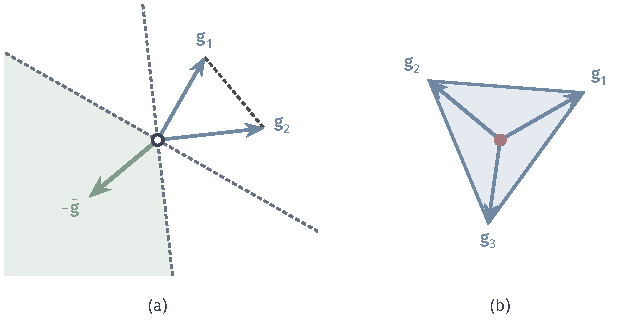
\includegraphics[width=104.8mm]{figures/05-optimization/07-multiple-criteria-and-nested-optimization/tikz/moo-common-descent/figure.pdf}
  \caption{共同下降方向与梯度的凸包，空心点和红点是原点。(a)两个梯度的凸包是虚线线段，不含原点；两条灰色虚线分别垂直于$\bm{g}_1,\bm{g}_2$，绿色楔形是共同下降方向。(b)三个梯度的凸包是浅蓝三角形，原点（红点）在其内部，此时不存在共同下降方向。}
  \label{fig:moo-common-descent}
\end{BookInlineFigure}

\paragraph{用梯度的凸包判别}
图~\ref{fig:moo-common-descent}提示了判别方法。把各梯度当作点，看它们的\term{凸包}（convex hull）
\[
 \operatorname{conv}\{\bm{g}_1,\ldots,\bm{g}_m\}=\Bigl\{\sum_{i=1}^m\theta_i\bm{g}_i:\bm{\theta}\in\Delta_m\Bigr\},
\]
也就是全部梯度的加权平均组成的集合。下面的引理说，这个集合是否包含原点，恰好决定共同下降方向是否存在。

\begin{lemma}[共同下降方向的存在性]
\label{lem:moo-gordan}
存在满足式~\eqref{eq:moo-common-descent}的$\bm{d}$，当且仅当$\bm{0}\notin\operatorname{conv}\{\bm{g}_1,\ldots,\bm{g}_m\}$。
\end{lemma}

\begin{proof}
先设$\bm{0}$在凸包中，即有$\bm{\theta}\in\Delta_m$使$\sum_i\theta_i\bm{g}_i=\bm{0}$。若式~\eqref{eq:moo-common-descent}成立，把它们按$\theta_i\geq0$加权相加，由于至少有一个$\theta_i>0$，得到
\[
 0=\Bigl\langle\sum_i\theta_i\bm{g}_i,\bm{d}\Bigr\rangle=\sum_i\theta_i\langle\bm{g}_i,\bm{d}\rangle<0,
\]
矛盾。

再设$\bm{0}$不在凸包中。凸包是非空紧凸集，记原点在它上面的投影为$\bar{\bm{g}}\neq\bm{0}$。第~\ref{chap:nonsmooth-composite-optimization}章的投影性质给出，对凸包中任一点$\bm{v}$，
\[
 \langle\bm{0}-\bar{\bm{g}},\bm{v}-\bar{\bm{g}}\rangle\leq0.
\]
取$\bm{v}=\bm{g}_i$，整理得
\[
 \langle\bm{g}_i,\bar{\bm{g}}\rangle\geq\lVert\bar{\bm{g}}\rVert_2^2>0.
\]
令$\bm{d}=-\bar{\bm{g}}$，式~\eqref{eq:moo-common-descent}成立。
\end{proof}

第二部分的构造不只是存在性证明，第~\ref{sec:moo-mgda}节就要把它变成算法。原点在凸包中的情形有专门的名称。

\begin{definition}[Pareto驻定]
\label{def:moo-stationary}
若存在$\bm{\theta}\in\Delta_m$，使
\begin{equation}
 \sum_{i=1}^m\theta_i\nabla f_i(\bm{x})=\bm{0},
 \label{eq:moo-stationary}
\end{equation}
称$\bm{x}$为\term{Pareto驻定}（Pareto stationary）点。
\end{definition}

$m=1$时，$\theta_1=1$，式~\eqref{eq:moo-stationary}就是$\nabla f_1=\bm{0}$，回到单目标的驻定点。多目标时，并不要求每个梯度为零，只要求它们能以非负系数相互抵消。

\paragraph{必要性与连续例}
局部最优点不允许共同下降，由此得到一阶必要条件。

\begin{theorem}[Pareto驻定的必要性]
\label{thm:moo-stationary-necessary}
设$\bm{x}$是$\bm{C}$的内点，各$f_i$在$\bm{x}$处可微。若$\bm{x}$是局部弱Pareto最优点，特别地若$\bm{x}$是局部Pareto最优点，则$\bm{x}$是Pareto驻定点。
\end{theorem}

\begin{proof}
若$\bm{x}$不是Pareto驻定点，由引理~\ref{lem:moo-gordan}，存在满足式~\eqref{eq:moo-common-descent}的$\bm{d}$。对充分小的$t>0$，由Taylor展开，
\[
 f_i(\bm{x}+t\bm{d})=f_i(\bm{x})+t\langle\bm{g}_i,\bm{d}\rangle+o(t)<f_i(\bm{x})
\]
对所有$i$成立。$\bm{x}$是内点，$\bm{x}+t\bm{d}$可行，这与局部弱Pareto最优矛盾。
\end{proof}

下面在例~\eqref{eq:moo-iso}上检查，见图~\ref{fig:moo-gradient-points}。此时$\bm{g}_1=\bm{x}-\bm{a}$，$\bm{g}_2=\bm{x}-\bm{b}$。在线段外的点$\bm{p}=(1,1)$处，
\[
 \bm{g}_1=(0,1),\qquad\bm{g}_2=(1,0).
\]
它们的凸组合是$(1-\theta,\theta)$，永远不为零，所以$\bm{p}$不是驻定点。取$\theta=1/2$得最短的组合$(1/2,1/2)$，方向$\bm{d}=(-1/2,-1/2)$使两个目标同时下降。

在线段上的点$\bm{q}=(0.6,0.4)$处，
\[
 \bm{g}_1=(-0.4,0.4),\qquad\bm{g}_2=(0.6,-0.6).
\]
两个梯度方向相反，取$\bm{\theta}=(0.6,0.4)$得到$0.6\bm{g}_1+0.4\bm{g}_2=\bm{0}$，$\bm{q}$是驻定点。这里的$\theta_1=0.6$恰好等于式~\eqref{eq:moo-iso-weighted}中选中$\bm{q}$的权重$w$。

\begin{BookInlineFigure}
  \centering
  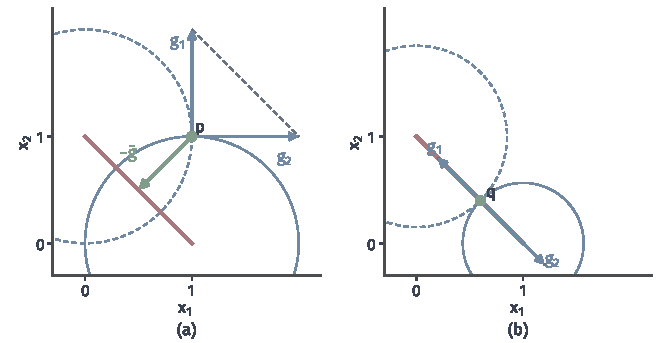
\includegraphics[width=112mm]{figures/05-optimization/07-multiple-criteria-and-nested-optimization/matplotlib/moo-gradient-points/figure.pdf}
  \caption{例~\eqref{eq:moo-iso}中两点处的梯度，圆是经过该点的两条等高线，红色线段是Pareto解集。(a)线段外的点$\bm{p}=(1,1)$，两个梯度的凸包（虚线）不含零，绿色箭头是最小范数组合的反方向。(b)线段上的点$\bm{q}=(0.6,0.4)$，两个梯度反向，凸包含零，两条等高线在$\bm{q}$相切。}
  \label{fig:moo-gradient-points}
\end{BookInlineFigure}

图~\ref{fig:moo-gradient-points}(b)还显示了一件事：在$\bm{q}$处两个圆相切，要进入一个圆的内部，就必须走出另一个圆。这是取舍的局部形象。

\paragraph{驻定点不一定是Pareto最优点}
定理~\ref{thm:moo-stationary-necessary}只有一个方向。Pareto驻定只排除严格的共同下降，并不排除“有的目标不变，另一些目标下降”。取$\bm{x}\in\mathbb{R}^2$，
\begin{equation}
 f_1(\bm{x})=x_1^2,\qquad f_2(\bm{x})=x_2.
 \label{eq:moo-stationary-weak}
\end{equation}
在原点，$\bm{g}_1=\bm{0}$，$\bm{g}_2=(0,1)$，取$\bm{\theta}=(1,0)$，式~\eqref{eq:moo-stationary}成立。可是沿$(0,-t)$移动，$f_1$保持为$0$，$f_2$严格下降，原点被支配，见图~\ref{fig:moo-stationary-gap}(a)。

问题还可能更严重。取一元函数$f_1(x)=f_2(x)=-x^2$，$x=0$是Pareto驻定点，但$x=\pm1$处两个目标都更小，原点连弱Pareto最优点都不是，见图~\ref{fig:moo-stationary-gap}(b)。这与单目标的极大点也是驻定点是同一回事。

\begin{BookInlineFigure}
  \centering
  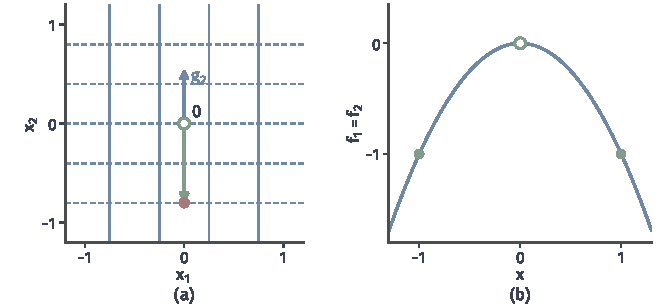
\includegraphics[width=112mm]{figures/05-optimization/07-multiple-criteria-and-nested-optimization/matplotlib/moo-stationary-gap/figure.pdf}
  \caption{Pareto驻定不足以断定最优。(a)式~\eqref{eq:moo-stationary-weak}，竖线是$f_1$的等高线，虚线是$f_2$的等高线；在空心点（原点）处$\bm{g}_1=\bm{0}$，沿绿色箭头$f_1$不变、$f_2$下降，红点支配原点。(b)$f_1=f_2=-x^2$，空心点是驻定点，两个绿点的目标都更小。}
  \label{fig:moo-stationary-gap}
\end{BookInlineFigure}

\paragraph{凸问题中的充分性}
要从驻定走到最优，需要凸性。此时式~\eqref{eq:moo-stationary}的系数$\bm{\theta}$恰好提供了一组权重。

\begin{theorem}[凸问题的驻定点]
\label{thm:moo-stationary-sufficient}
设$\bm{C}=\mathbb{R}^n$，各$f_i$凸且可微，$\bm{x}$满足式~\eqref{eq:moo-stationary}。则$\bm{x}$是$\sum_i\theta_if_i$的全局最小点，因而是全局弱Pareto最优点；若所有$\theta_i>0$，$\bm{x}$是全局Pareto最优点。
\end{theorem}

\begin{proof}
$\sum_i\theta_if_i$是凸函数，其梯度在$\bm{x}$处为零，由第~\ref{chap:optimization}章的一阶条件，$\bm{x}$是它的全局最小点。再由定理~\ref{thm:moo-weighted}得结论。
\end{proof}

式~\eqref{eq:moo-stationary-weak}的原点符合定理的条件，但$\theta_2=0$，所以只能得到弱Pareto最优，这正好和前面看到的现象一致。在例~\eqref{eq:moo-iso}的线段内部，$\bm{\theta}$的两个分量都为正，得到的是Pareto最优。

\subsection{可行方向}
\label{sec:moo-feasible-direction}

候选点若在可行集边界上，只有一部分方向走得动，梯度的凸包不含零也不等于存在可行的共同下降方向。这一小节把判别限制在可行方向上，并调用第~\ref{chap:constrained-optimality}章的约束条件。

\paragraph{问题与记号}
由于$m$已经用来表示目标个数，约束的下标改写为
\[
 \bm{C}=\{\bm{x}:g_j(\bm{x})\leq0,\ j=1,\ldots,q,\ \ h_k(\bm{x})=0,\ k=1,\ldots,p\}.
\]
活动集$A(\bar{\bm{x}})$、切锥$\bm{T}_{\bm{C}}(\bar{\bm{x}})$、线性化锥、LICQ、MFCQ的含义都与第~\ref{chap:constrained-optimality}章相同，只是把不等式的下标换成了$j$，等式的下标换成了$k$。这里的$g_j$是约束函数，加粗的$\bm{g}_i$才是目标的梯度。

\paragraph{切锥上的必要条件}
“能走的方向”由切锥描述，一阶必要条件的形式与单目标的切锥条件相同。

\begin{theorem}[切锥上的必要条件]
\label{thm:moo-tangent-necessary}
设$\bar{\bm{x}}$是局部弱Pareto最优点，各$f_i$在$\bar{\bm{x}}$处可微。则不存在$\bm{d}\in\bm{T}_{\bm{C}}(\bar{\bm{x}})$，使
\begin{equation}
 \langle\nabla f_i(\bar{\bm{x}}),\bm{d}\rangle<0\quad\text{对所有}\ i=1,\ldots,m.
 \label{eq:moo-tangent-descent}
\end{equation}
\end{theorem}

\begin{proof}
设这样的$\bm{d}$存在。由切锥定义，有可行点列$\bm{x}^{(k)}\to\bar{\bm{x}}$与$t_k\downarrow0$，使$(\bm{x}^{(k)}-\bar{\bm{x}})/t_k\to\bm{d}$。Taylor展开并除以$t_k$，
\[
 \frac{f_i(\bm{x}^{(k)})-f_i(\bar{\bm{x}})}{t_k}\to\langle\nabla f_i(\bar{\bm{x}}),\bm{d}\rangle<0.
\]
目标个数有限，所以$k$足够大时，所有$f_i(\bm{x}^{(k)})<f_i(\bar{\bm{x}})$同时成立，与局部弱Pareto最优矛盾。
\end{proof}

\paragraph{目标权重与约束乘子}
切锥不容易计算。约束资格把它换成线性化锥，结论就可以用乘子写出来，形式上是把KKT条件中目标的梯度换成目标梯度的凸组合。

证明不用重新做Farkas那一套，把问题改写成单目标问题即可：引入一个变量$t$代表“所有目标相对当前点的最大变化”，然后要求这个变化不能为负。

\begin{theorem}[多目标KKT必要条件]
\label{thm:moo-kkt-necessary}
设$f_i$、$g_j$、$h_k$在局部弱Pareto最优点$\bar{\bm{x}}$附近连续可微，并且$\bar{\bm{x}}$满足MFCQ。则存在$\bm{\theta}\in\Delta_m$，$\bm{\lambda}\geq\bm{0}$，$\bm{\nu}$，使
\begin{equation}
 \sum_{i=1}^m\theta_i\nabla f_i(\bar{\bm{x}})
 +\sum_{j=1}^q\lambda_j\nabla g_j(\bar{\bm{x}})
 +\sum_{k=1}^p\nu_k\nabla h_k(\bar{\bm{x}})=\bm{0},
 \label{eq:moo-kkt}
\end{equation}
并且$\lambda_jg_j(\bar{\bm{x}})=0$对所有$j$成立。
\end{theorem}

\begin{proof}
考虑变量为$(\bm{x},t)$的单目标问题
\[
 \min_{\bm{x},t}\ t\quad\text{s.t.}\quad
 f_i(\bm{x})-f_i(\bar{\bm{x}})-t\leq0,\ \ \bm{x}\in\bm{C}.
\]

先说明$(\bar{\bm{x}},0)$是它的局部最小点。若$\bm{x}$靠近$\bar{\bm{x}}$，$(\bm{x},t)$可行且$t<0$，则$f_i(\bm{x})<f_i(\bar{\bm{x}})$对所有$i$成立，与局部弱Pareto最优矛盾。

再说明MFCQ在$(\bar{\bm{x}},0)$处成立。设$\bar{\bm{d}}$是原约束的MFCQ方向。增广问题中等式约束的梯度是$(\nabla h_k,0)$，线性无关；取方向$(\bar{\bm{d}},\sigma)$，$\sigma$足够大，则
\[
 \langle\nabla f_i(\bar{\bm{x}}),\bar{\bm{d}}\rangle-\sigma<0\quad\text{对所有}\ i,
\]
其余条件与原约束相同。

由第~\ref{chap:constrained-optimality}章的KKT必要性定理，存在乘子$\bm{\theta}\geq\bm{0}$（对应$f_i-f_i(\bar{\bm{x}})-t\leq0$）、$\bm{\lambda}\geq\bm{0}$与$\bm{\nu}$。对$t$的驻定条件是$1-\sum_i\theta_i=0$，所以$\bm{\theta}\in\Delta_m$；对$\bm{x}$的驻定条件是式~\eqref{eq:moo-kkt}；互补条件来自原约束的互补松弛。
\end{proof}

约束资格不能省。取一元变量，$f_1(x)=f_2(x)=x$，约束$g(x)=x^2\leq0$。可行集只有$\{0\}$，所以$0$是Pareto最优点。但$\nabla f_1=\nabla f_2=1$，$\nabla g(0)=0$，式~\eqref{eq:moo-kkt}左边恒等于$1$。这里MFCQ失败，因为$\langle\nabla g(0),d\rangle=0$，不可能严格小于零。

\paragraph{凸问题中的充分性}
和无约束情形一样，充分性需要凸性，而且权重的符号决定结论的强弱。

\begin{theorem}[凸问题的多目标KKT充分性]
\label{thm:moo-kkt-sufficient}
设$\bm{D}$是包含$\bm{C}$的开凸集，$f_i$、$g_j$在$\bm{D}$上凸且可微，$h_k$仿射。若可行点$\bar{\bm{x}}$满足式~\eqref{eq:moo-kkt}，$\bm{\theta}\in\Delta_m$，$\bm{\lambda}\geq\bm{0}$，且互补松弛成立，则$\bar{\bm{x}}$是$\sum_i\theta_if_i$在$\bm{C}$上的全局最小点，因而是全局弱Pareto最优点；若所有$\theta_i>0$，$\bar{\bm{x}}$是全局Pareto最优点。
\end{theorem}

\begin{proof}
式~\eqref{eq:moo-kkt}与互补松弛正是凸问题$\min_{\bm{C}}\sum_i\theta_if_i$的KKT条件。由第~\ref{chap:constrained-optimality}章的凸问题KKT充分性，$\bar{\bm{x}}$是全局最小点。再由定理~\ref{thm:moo-weighted}得结论。
\end{proof}

这里没有要求约束资格，这与单目标的凸问题相同。必要性要约束资格而不要凸性，充分性要凸性而不要约束资格，两个方向的条件不能互换。

\paragraph{例：无约束判据为什么失效}
在例~\eqref{eq:moo-iso}上加一个约束$g(\bm{x})=x_1+x_2-1/2\leq0$。原来的解集$x_1+x_2=1$整条被挡在可行集外面，新的候选应该在边界上。取$\bar{\bm{x}}=(1/4,1/4)$，
\[
 \bm{g}_1=\bar{\bm{x}}-\bm{a}=(-3/4,1/4),\qquad\bm{g}_2=\bar{\bm{x}}-\bm{b}=(1/4,-3/4).
\]

这两个梯度的凸包不含零。取$\bm{\theta}=(1/2,1/2)$得到其中最短的组合
\[
 \bar{\bm{g}}=(-1/4,-1/4).
\]
如果套用无约束判据，就会以为$\bar{\bm{x}}$不是驻定点。可是下降方向$-\bar{\bm{g}}=(1/4,1/4)$走出了可行集，这一步根本走不了。

加上约束的乘子就对了。由式~\eqref{eq:moo-kkt}，$\nabla g=(1,1)$，
\[
 \tfrac12\bm{g}_1+\tfrac12\bm{g}_2+\lambda(1,1)=\bm{0},
\]
解得$\lambda=1/4\geq0$。$\bar{\bm{x}}$在边界上，互补松弛成立，问题是凸的，权重全正，由定理~\ref{thm:moo-kkt-sufficient}，$\bar{\bm{x}}$是全局Pareto最优点。

更一般地，式~\eqref{eq:moo-kkt}对可行点$\bm{x}$写出来是$\bm{x}=(\theta-\lambda,1-\theta-\lambda)$，其中$\bm{\theta}=(\theta,1-\theta)$。边界条件$x_1+x_2=1/2$给出$\lambda=1/4$，所以约束问题的驻定点是
\begin{equation}
 \bm{x}=\bigl(\theta-\tfrac14,\ \tfrac34-\theta\bigr),\qquad 0\leq\theta\leq1.
 \label{eq:moo-feasible-set}
\end{equation}

代入目标，前沿是$\bigl((1-\theta)^2+\tfrac1{16},\ \theta^2+\tfrac1{16}\bigr)$，恰是原前沿沿两个方向平移$1/16$。图~\ref{fig:moo-feasible-pareto}把解集和前沿画了出来。

\begin{BookInlineFigure}
  \centering
  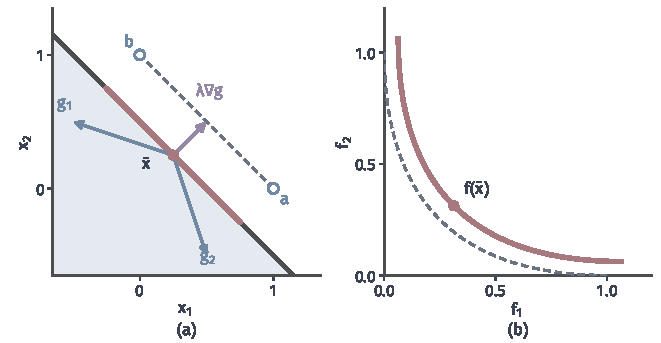
\includegraphics[width=112mm]{figures/05-optimization/07-multiple-criteria-and-nested-optimization/matplotlib/moo-feasible-pareto/figure.pdf}
  \caption{加上半平面约束$x_1+x_2\leq1/2$后的例子。(a)深灰粗线是活动约束，红色线段是约束下的解集（式~\eqref{eq:moo-feasible-set}），虚线是原来的解集；在$\bar{\bm{x}}=(1/4,1/4)$处，$\bm{g}_1,\bm{g}_2$的中点被紫色的$\lambda\nabla g$抵消。(b)红色曲线是约束下的前沿，虚线是原前沿，红点是$\bm{f}(\bar{\bm{x}})=(5/16,5/16)$。}
  \label{fig:moo-feasible-pareto}
\end{BookInlineFigure}

端点$\theta=0,1$的权重有零，但此时分别是$f_2$、$f_1$在可行集上的唯一最小点，由定理~\ref{thm:moo-weighted}的第~3条仍是Pareto最优点。这说明定理~\ref{thm:moo-kkt-sufficient}中“全正”只是充分条件，端点要单独检查。

\section{多梯度下降}
\label{sec:moo-mgda}

第~\ref{sec:moo-common-descent}节的判别给出了一个方向：梯度凸包中离原点最近的点。这一节把它变成迭代。问题是：怎样在几个目标的梯度之间取折中，才能保证一步之后每个目标都不变差？

由此得到的方法称为\term{多梯度下降算法}（multiple-gradient descent algorithm，MGDA）。它不需要事先给定偏好，权重是每一步按当前的几何现算的，这一点和固定加权和不同。

\subsection{最小范数组合}
\label{sec:moo-min-norm}

\paragraph{主要思想}
最简单的想法是把各目标的梯度平均一下，然后沿反方向走。看一个具体的数据：
\[
 \bm{g}_1=(10,1),\qquad\bm{g}_2=(-1,1).
\]
平均后得$(4.5,1)$，方向是$\bm{d}=(-4.5,-1)$。检查第二个目标的方向导数：
\[
 \langle\bm{g}_2,\bm{d}\rangle=4.5-1=3.5>0.
\]
$f_2$反而上升。梯度长度悬殊时，长的那个梯度支配了平均，短的那个目标被牺牲了。

\begin{BookInlineFigure}
  \centering
  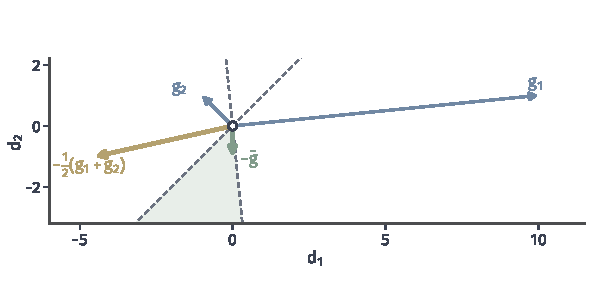
\includegraphics[width=100mm]{figures/05-optimization/07-multiple-criteria-and-nested-optimization/matplotlib/moo-average-vs-minnorm/figure.pdf}
  \caption{平均方向与最小范数方向，$\bm{g}_1=(10,1)$，$\bm{g}_2=(-1,1)$。两条灰色虚线分别垂直于两个梯度，浅绿楔形是共同下降方向。黄色箭头是平均梯度的反方向，落在楔形外；绿色箭头是$-\bar{\bm{g}}=(0,-1)$，落在楔形内。}
  \label{fig:moo-average-vs-minnorm}
\end{BookInlineFigure}

要保证每个目标都下降，应当转而问：在所有梯度的加权平均中，哪一个最短？记
\begin{equation}
 \bm{\theta}^\star\in\argmin_{\bm{\theta}\in\Delta_m}\ \frac12\Bigl\lVert\sum_{i=1}^m\theta_i\bm{g}_i\Bigr\rVert_2^2,
 \qquad
 \bar{\bm{g}}=\sum_{i=1}^m\theta_i^\star\bm{g}_i,
 \label{eq:moo-min-norm}
\end{equation}
并取方向$\bm{d}=-\bar{\bm{g}}$。式~\eqref{eq:moo-min-norm}的权重子问题在单纯形上最小化一个凸二次函数。$\bar{\bm{g}}$是原点在凸包上的投影，所以唯一，而$\bm{\theta}^\star$不一定唯一。

在上面的数据上，后面的式~\eqref{eq:moo-theta-two}给出$\theta_1^\star=1/11$，于是$\bar{\bm{g}}=(0,1)$，方向$(0,-1)$落在共同下降的楔形内，见图~\ref{fig:moo-average-vs-minnorm}。两个方向导数都等于$-1$。

\begin{lemma}[最小范数组合的下降性质]
\label{lem:moo-min-norm}
对式~\eqref{eq:moo-min-norm}定义的$\bar{\bm{g}}$，
\begin{equation}
 \langle\bm{g}_i,-\bar{\bm{g}}\rangle\leq-\lVert\bar{\bm{g}}\rVert_2^2\quad\text{对所有}\ i=1,\ldots,m.
 \label{eq:moo-min-norm-descent}
\end{equation}
并且$\bar{\bm{g}}=\bm{0}$当且仅当$\bm{x}$是无约束的Pareto驻定点。
\end{lemma}

\begin{proof}
不等式已在引理~\ref{lem:moo-gordan}的证明中得到，投影性质给出
\[
 \langle\bm{g}_i,\bar{\bm{g}}\rangle\geq\lVert\bar{\bm{g}}\rVert_2^2,
\]
这对$\bar{\bm{g}}=\bm{0}$也成立。第二句是Pareto驻定的定义：$\bm{0}$在凸包中，当且仅当它到凸包的最短距离为零。
\end{proof}

式~\eqref{eq:moo-min-norm-descent}是整个方法的关键：只要$\bar{\bm{g}}\neq\bm{0}$，每个目标的方向导数都不大于$-\lVert\bar{\bm{g}}\rVert_2^2$，都确实在下降，而且下降速度有统一的下界。

\paragraph{两个目标的闭式解}
$m=2$时，令$\bm{\theta}=(\theta,1-\theta)$，$\bm{g}_1\neq\bm{g}_2$。子问题是一元二次函数：
\[
 \phi(\theta)=\lVert\theta\bm{g}_1+(1-\theta)\bm{g}_2\rVert_2^2=\lVert\bm{g}_2+\theta(\bm{g}_1-\bm{g}_2)\rVert_2^2.
\]
求导令其为零，得到无约束的最小点$\langle\bm{g}_2,\bm{g}_2-\bm{g}_1\rangle/\lVert\bm{g}_1-\bm{g}_2\rVert_2^2$。把它截断到$[0,1]$，由于$\phi$是凸的一元二次函数，截断后仍是区间上的最小点：
\begin{equation}
 \theta^\star=\min\Bigl\{1,\ \max\Bigl\{0,\ \frac{\langle\bm{g}_2,\bm{g}_2-\bm{g}_1\rangle}{\lVert\bm{g}_1-\bm{g}_2\rVert_2^2}\Bigr\}\Bigr\}.
 \label{eq:moo-theta-two}
\end{equation}
若$\bm{g}_1=\bm{g}_2$，任取$\theta$都得到同一个$\bar{\bm{g}}$。

图~\ref{fig:moo-min-norm}是三种情形。(a)垂足落在线段内部，$0<\theta^\star<1$，此时式~\eqref{eq:moo-min-norm-descent}对两个目标都取等号，两个目标下降速度相同。(b)垂足落在线段之外，截断后$\bar{\bm{g}}$就是较短的梯度，方向只对那一个目标是最陡的，另一个目标下降得更快。(c)原点在线段上，$\bar{\bm{g}}=\bm{0}$，停止。

\begin{BookInlineFigure}
  \centering
  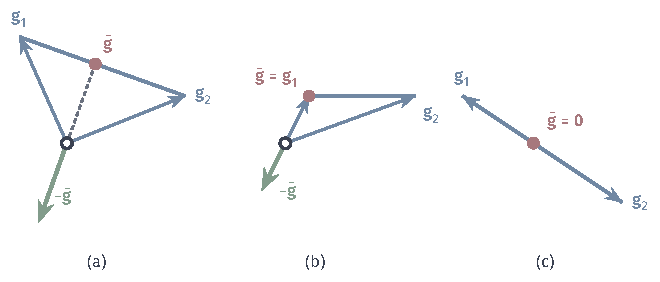
\includegraphics[width=111.8mm]{figures/05-optimization/07-multiple-criteria-and-nested-optimization/tikz/moo-min-norm/figure.pdf}
  \caption{两个梯度的最小范数组合。蓝色线段是凸包，红点是$\bar{\bm{g}}$，绿色箭头是$-\bar{\bm{g}}$，空心点是原点。(a)垂足在线段内部。(b)垂足在线段外，截断到较短的梯度$\bm{g}_1$。(c)原点在线段上，点是Pareto驻定的，没有更新方向。}
  \label{fig:moo-min-norm}
\end{BookInlineFigure}

\paragraph{方向的最优性}
最小范数这个构造还可以从另一面看：它正好是一个“保最差目标”的方向问题的解。假设只看一阶模型，希望下降最少的目标也尽量下降，同时用$\frac12\lVert\bm{d}\rVert_2^2$防止步子过大。

\begin{theorem}[最坏目标的最陡方向]
\label{thm:moo-steepest}
问题
\begin{equation}
 \min_{\bm{d}\in\mathbb{R}^n}\ \max_{1\leq i\leq m}\langle\bm{g}_i,\bm{d}\rangle+\frac12\lVert\bm{d}\rVert_2^2
 \label{eq:moo-steepest}
\end{equation}
的唯一解是$\bm{d}=-\bar{\bm{g}}$，最优值是$-\frac12\lVert\bar{\bm{g}}\rVert_2^2$。
\end{theorem}

\begin{proof}
目标是凸函数加强凸函数，解唯一。对任意$\bm{d}$，最大值不小于凸组合，所以
\[
 \max_i\langle\bm{g}_i,\bm{d}\rangle+\tfrac12\lVert\bm{d}\rVert_2^2
 \geq\langle\bar{\bm{g}},\bm{d}\rangle+\tfrac12\lVert\bm{d}\rVert_2^2.
\]
右端关于$\bm{d}$的最小值在$\bm{d}=-\bar{\bm{g}}$取到，所以
\[
 \max_i\langle\bm{g}_i,\bm{d}\rangle+\tfrac12\lVert\bm{d}\rVert_2^2
 \geq-\tfrac12\lVert\bar{\bm{g}}\rVert_2^2.
\]

反过来，取$\bm{d}=-\bar{\bm{g}}$，由式~\eqref{eq:moo-min-norm-descent}，最大值不超过$-\lVert\bar{\bm{g}}\rVert_2^2$，目标不超过$-\frac12\lVert\bar{\bm{g}}\rVert_2^2$。两边合起来取等，$-\bar{\bm{g}}$是解。
\end{proof}

\paragraph{权重的含义}
$\bm{\theta}^\star$看起来也是一组权重，但它与加权和的权重$\bm{w}$职责不同，见表~\ref{tab:moo-weights}。$\bm{w}$是决策者给定的，整个求解过程中不变，表达的是偏好。$\bm{\theta}^\star$是算法每一步根据当前梯度算出来的，表达的是当前的几何。

\begin{BookInlineTable}
  \centering
  \caption{固定加权与多梯度下降中的权重。}
  \label{tab:moo-weights}
  \begin{tabular}{@{}lll@{}}
    \toprule
     & 加权和的$\bm{w}$ & 多梯度下降的$\bm{\theta}^\star$\\
    \midrule
    来源 & 使用者事先给定 & 每步由梯度算出\\
    迭代中 & 固定 & 随$\bm{x}$变化\\
    单个目标 & 可能上升 & 不上升（配合步长）\\
    终点 & 该偏好下的解 & 取决于起点的一个驻定点\\
    \bottomrule
  \end{tabular}
\end{BookInlineTable}

要注意$\bm{\theta}^\star$不是尺度无关的。把上面的$f_1$除以$10$，$\bm{g}_1$变成$(1,0.1)$，由式~\eqref{eq:moo-theta-two}算得$\theta^\star\approx0.603$，$\bar{\bm{g}}\approx(0.206,0.457)$，方向和原来的$(0,1)$不同。所以第~\ref{sec:moo-scale}节的提醒在这里同样适用：梯度长度悬殊的问题，先要说明目标的尺度。

$m>2$时，令$\bm{G}$是$m\times m$矩阵，元素为$\bm{G}_{i,j}=\langle\bm{g}_i,\bm{g}_j\rangle$，子问题就是在单纯形上最小化$\frac12\bm{\theta}^\top\bm{G}\bm{\theta}$。第~\ref{chap:quadratic-conic-programming}章的二次规划方法和第~\ref{chap:feasible-iterations}章的Frank--Wolfe方法都能解它。单纯形的规模只有$m$，主要开销在于计算$m$个梯度和$\bm{G}$的$O(m^2n)$次运算。

\subsection{共同步长}
\label{sec:moo-common-step}

有了方向，还要决定走多远。若沿各自的梯度分别走一步，再把得到的位置取平均，效果等同于沿平均梯度走一步，前面已经看到这可能让某个目标上升。所以这一小节要为所有目标选一个共同的步长，并检查每一个目标的下降。

\paragraph{多目标的充分下降}
把单目标的回溯规则（第~\ref{chap:smooth-foundations}章）推广：一个步长$\alpha>0$只有在所有目标都达到下面的下降量时才被接受，
\begin{equation}
 f_i(\bm{x}-\alpha\bar{\bm{g}})\leq f_i(\bm{x})-c\,\alpha\lVert\bar{\bm{g}}\rVert_2^2\quad\text{对所有}\ i,
 \label{eq:moo-armijo}
\end{equation}
其中$c\in(0,1)$，常取$c=1/2$。回溯时从$\alpha=1$开始，不满足就乘以$\beta\in(0,1)$，这里取$\beta=1/2$。

为什么步长一定找得到？设每个$\nabla f_i$是$L_i$-Lipschitz的，记$L_{\max}=\max_iL_i$。由下降引理（第~\ref{chap:smooth-foundations}章）和式~\eqref{eq:moo-min-norm-descent}，
\[
 f_i(\bm{x}-\alpha\bar{\bm{g}})
 \leq f_i(\bm{x})+\alpha\langle\bm{g}_i,-\bar{\bm{g}}\rangle+\frac{L_i\alpha^2}{2}\lVert\bar{\bm{g}}\rVert_2^2
 \leq f_i(\bm{x})-\alpha\Bigl(1-\frac{L_i\alpha}{2}\Bigr)\lVert\bar{\bm{g}}\rVert_2^2.
\]
所以当$\alpha\leq1/L_{\max}$时，括号不小于$1/2$，式~\eqref{eq:moo-armijo}在$c=1/2$时成立。

从这里也看得出共同步长的代价：步长受曲率最大的那个目标限制，$L_{\max}$很大时所有目标都得小步前进。

\paragraph{计算过程}
下面在一个病态的例子上走三轮。目标的第一项是第~\ref{chap:smooth-foundations}章贯穿使用的二次函数，第二项把点拉向$(4,3)$：
\begin{equation}
 f_1(\bm{x})=\frac12(x_1^2+9x_2^2),\qquad
 f_2(\bm{x})=\frac12\bigl[(x_1-4)^2+(x_2-3)^2\bigr].
 \label{eq:moo-mgda-example}
\end{equation}

\needspace{6\baselineskip}
\paragraph{变量}
\begin{itemize}
 \item 迭代点$\bm{x}^{(t)}\in\mathbb{R}^n$，各目标的值$f_i(\bm{x}^{(t)})$；
 \item 梯度$\bm{g}_i^{(t)}=\nabla f_i(\bm{x}^{(t)})$，$i=1,\ldots,m$；
 \item 组合系数$\bm{\theta}^{(t)}\in\Delta_m$，组合梯度$\bar{\bm{g}}^{(t)}$；
 \item 步长$\alpha^{(t)}$，常数$c$、$\beta$，容差$\epsilon$。
\end{itemize}

\paragraph{初始化}
给定起点$\bm{x}^{(0)}$和容差$\epsilon$。例中取$\bm{x}^{(0)}=(1,1)$，$c=\beta=1/2$，此时目标值为
\[
 \bm{f}(\bm{x}^{(0)})=(5,\ 6.5).
\]

\paragraph{每轮更新}
对$t=0,1,\ldots$重复下列步骤，直到$\lVert\bar{\bm{g}}^{(t)}\rVert_2\leq\epsilon$。

\begin{enumerate}
 \item 计算各目标的梯度。例中第一轮
 \[
  \bm{g}_1^{(0)}=(1,9),\qquad\bm{g}_2^{(0)}=(-3,-2).
 \]

 \item 由式~\eqref{eq:moo-min-norm}求$\bm{\theta}^{(t)}$与$\bar{\bm{g}}^{(t)}$，两个目标时用式~\eqref{eq:moo-theta-two}。例中第一轮
 \[
  \theta^{(0)}=\frac{34}{137}\approx0.2482,\qquad
  \bar{\bm{g}}^{(0)}\approx(-2.0073,\ 0.7299),
 \]
 并且$\lVert\bar{\bm{g}}^{(0)}\rVert_2^2\approx4.5620$。

 \item 回溯求步长：从$\alpha=1$开始，检查式~\eqref{eq:moo-armijo}是否对每一个目标成立。例中$\alpha=1$的试探点是$(3.0073,0.2701)$，$f_1\approx4.8501$，而要求不超过$5-\frac12\times4.5620\approx2.7190$，被拒绝。$\alpha=1/2$的试探点满足两个目标的要求：
 \[
  f_1\approx3.8220\leq3.8595,\qquad f_2\approx4.7892\leq5.3595.
 \]

 \item 沿$-\bar{\bm{g}}^{(t)}$走一步，更新为
 \begin{equation}
  \bm{x}^{(t+1)}=\bm{x}^{(t)}-\alpha^{(t)}\bar{\bm{g}}^{(t)}.
  \label{eq:moo-mgda-update}
 \end{equation}
 例中第一轮
 \[
  \bm{x}^{(1)}\approx(2.0036,\ 0.6350),\qquad
  \bm{f}(\bm{x}^{(1)})\approx(3.8220,\ 4.7892).
 \]
\end{enumerate}

第二轮的梯度是
\[
 \bm{g}_1^{(1)}\approx(2.0036,\ 5.7153),\qquad
 \bm{g}_2^{(1)}\approx(-1.9964,\ -2.3650).
\]
由此算得
\[
 \theta^{(1)}\approx0.3333,\quad
 \bar{\bm{g}}^{(1)}\approx(-0.6631,\ 0.3283),\quad
 \lVert\bar{\bm{g}}^{(1)}\rVert_2^2\approx0.5475.
\]
$\alpha=1$和$\alpha=1/2$都因$f_1$不满足式~\eqref{eq:moo-armijo}被拒绝，$\alpha=1/4$被接受，得到
\[
 \bm{x}^{(2)}\approx(2.1694,\ 0.5530),\qquad
 \bm{f}(\bm{x}^{(2)})\approx(3.7292,\ 4.6695).
\]

第三轮的梯度是
\[
 \bm{g}_1^{(2)}\approx(2.1694,\ 4.9767),\qquad
 \bm{g}_2^{(2)}\approx(-1.8306,\ -2.4470).
\]
算得
\[
 \theta^{(2)}\approx0.3584,\quad
 \bar{\bm{g}}^{(2)}\approx(-0.3969,\ 0.2138),\quad
 \lVert\bar{\bm{g}}^{(2)}\rVert_2^2\approx0.2032.
\]
同样$\alpha=1/4$被接受，
\[
 \bm{x}^{(3)}\approx(2.2687,\ 0.4995),\qquad
 \bm{f}(\bm{x}^{(3)})\approx(3.6962,\ 4.6250).
\]
可以看到，两个目标每一轮都严格下降，$\theta^{(t)}$在逐轮变化。

最终得到$\bm{x}^\star\approx(2.3933,0.4260)$，目标值约为$(3.6808,4.6034)$，$\bar{\bm{g}}$的范数已到舍入误差量级。这一点的$\theta^\star\approx0.4017$，用它作权重，第~\ref{sec:moo-weighted}节的加权和在这一点取到最优。

\begin{BookInlineFigure}
  \centering
  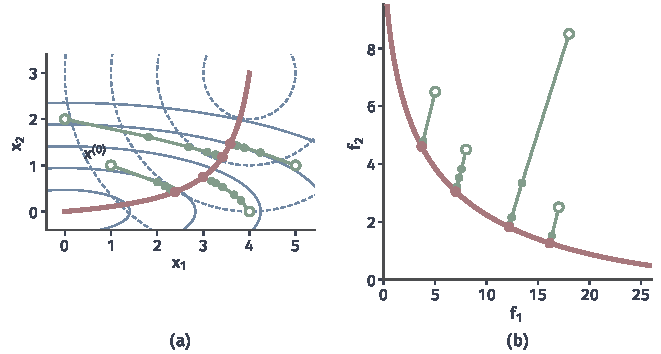
\includegraphics[width=112mm]{figures/05-optimization/07-multiple-criteria-and-nested-optimization/matplotlib/moo-mgda-path/figure.pdf}
  \caption{多梯度下降在例~\eqref{eq:moo-mgda-example}上的路径。(a)决策平面，实线与虚线分别是$f_1,f_2$的等高线，红色曲线是Pareto解集，绿线是四个起点（空心点）的路径，小点是前五步，红点是终点。(b)同一批路径在目标平面上的像，红色曲线是Pareto前沿。不同起点落到前沿的不同位置。}
  \label{fig:moo-mgda-path}
\end{BookInlineFigure}

\paragraph{收敛性}
图~\ref{fig:moo-mgda-path}显示，路径都在目标平面上朝左下方走，最后落到前沿上，不同起点落到不同位置。下面的定理说明能够保证的是什么。

\begin{theorem}[多梯度下降的收敛]
\label{thm:moo-mgda-convergence}
设每个$f_i$有下界$f_i^{\mathrm{low}}$，$\nabla f_i$是$L_i$-Lipschitz的，记$L_{\max}=\max_iL_i$。设迭代满足式~\eqref{eq:moo-armijo}，且$\alpha^{(t)}\geq\alpha_{\min}>0$。则对任意目标$i$和任意$T\geq1$，
\begin{equation}
 \min_{0\leq t<T}\lVert\bar{\bm{g}}^{(t)}\rVert_2^2
 \leq\frac{f_i(\bm{x}^{(0)})-f_i^{\mathrm{low}}}{c\,\alpha_{\min}T}.
 \label{eq:moo-mgda-rate}
\end{equation}
并且序列的每个极限点都是Pareto驻定点。固定步长$\alpha=1/L_{\max}$，$c=1/2$时满足条件，式~\eqref{eq:moo-mgda-rate}的右端为$2L_{\max}(f_i(\bm{x}^{(0)})-f_i^{\mathrm{low}})/T$。
\end{theorem}

\begin{proof}
由式~\eqref{eq:moo-armijo}，对每个$t$，
\[
 f_i(\bm{x}^{(t+1)})\leq f_i(\bm{x}^{(t)})-c\,\alpha_{\min}\lVert\bar{\bm{g}}^{(t)}\rVert_2^2.
\]
对$t=0,\ldots,T-1$求和，利用$f_i(\bm{x}^{(T)})\geq f_i^{\mathrm{low}}$，得到
\[
 c\,\alpha_{\min}\sum_{t=0}^{T-1}\lVert\bar{\bm{g}}^{(t)}\rVert_2^2\leq f_i(\bm{x}^{(0)})-f_i^{\mathrm{low}}.
\]
最小项不超过平均值，即得式~\eqref{eq:moo-mgda-rate}。这一和式也说明$\lVert\bar{\bm{g}}^{(t)}\rVert_2\to0$。

记$\varphi(\bm{x})$为点$\bm{x}$处的$\lVert\bar{\bm{g}}\rVert_2$。对任意$\bm{x},\bm{y}$，设$\bm{\theta}$是$\bm{y}$处的最优系数，
\[
 \varphi(\bm{x})\leq\Bigl\lVert\sum_i\theta_i\nabla f_i(\bm{x})\Bigr\rVert_2
 \leq\varphi(\bm{y})+L_{\max}\lVert\bm{x}-\bm{y}\rVert_2.
\]
交换$\bm{x},\bm{y}$，两式合起来给出
\[
 \lvert\varphi(\bm{x})-\varphi(\bm{y})\rvert\leq L_{\max}\lVert\bm{x}-\bm{y}\rVert_2,
\]
所以$\varphi$连续。沿收敛子列取极限，极限点处$\varphi=0$，由引理~\ref{lem:moo-min-norm}它是Pareto驻定点。

固定步长的情形由式~\eqref{eq:moo-armijo}之后的不等式给出。
\end{proof}

定理的结论是$\lVert\bar{\bm{g}}\rVert_2$趋于零，也就是逼近Pareto驻定。根据第~\ref{sec:moo-common-descent}节，这不等于全局Pareto最优；凸问题中，再加上极限处权重全正，才能推到Pareto最优。回溯时取$\alpha_{\min}=\min\{1,\beta/L_{\max}\}$即可满足定理的条件，因为一旦$\alpha\leq1/L_{\max}$就会被接受。

\paragraph{与固定加权的对比}
图~\ref{fig:moo-mgda-curves}比较了从$(4,0)$出发的两种迭代。这一点的目标值是$(8,4.5)$。固定权重$(1/2,1/2)$的梯度法（黄色）走向该偏好下的解$(2.41,5.64)$，$f_1$降了很多，但$f_2$从$4.5$升到了$5.64$。多梯度下降（绿色）停在$(6.99,3.04)$，两个目标都比起点好。

这两个结果没有谁对谁错。前者忠实地执行了“两项同样重要”的偏好，后者忠实地执行了“不让任何一项变差”的要求。一次运行得到的都只是前沿上的一个点。

\begin{BookInlineFigure}
  \centering
  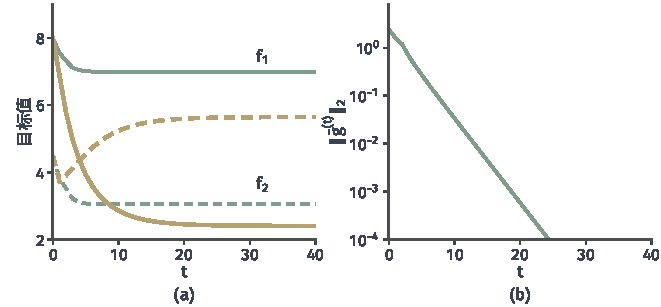
\includegraphics[width=112mm]{figures/05-optimization/07-multiple-criteria-and-nested-optimization/matplotlib/moo-mgda-curves/figure.pdf}
  \caption{从$(4,0)$出发的迭代，例~\eqref{eq:moo-mgda-example}。(a)实线是$f_1$，虚线是$f_2$，绿色是多梯度下降，黄色是固定权重$(1/2,1/2)$、步长$1/L$的梯度法，后者使$f_2$上升。(b)多梯度下降的$\lVert\bar{\bm{g}}^{(t)}\rVert_2$，纵轴为对数。}
  \label{fig:moo-mgda-curves}
\end{BookInlineFigure}

\paragraph{有约束时}
可行集$\bm{C}$是闭凸集时，把式~\eqref{eq:moo-steepest}限制到可行方向上：
\begin{equation}
 \bm{d}^{(t)}\in\argmin_{\bm{x}^{(t)}+\bm{d}\in\bm{C}}\ \max_i\langle\bm{g}_i^{(t)},\bm{d}\rangle+\frac12\lVert\bm{d}\rVert_2^2.
 \label{eq:moo-feasible-direction}
\end{equation}
$\bm{d}=\bm{0}$是可行的，目标值是$0$。由强凸性解唯一，所以$\bm{d}^{(t)}\neq\bm{0}$时最优值严格小于零，$\max_i\langle\bm{g}_i^{(t)},\bm{d}^{(t)}\rangle<0$，$\bm{d}^{(t)}$是共同下降方向。由$\bm{C}$凸，$\bm{x}^{(t)}+\alpha\bm{d}^{(t)}$在$\alpha\in(0,1]$时可行，沿它做共同步长的回溯即可。

反过来，若存在可行点$\bm{x}^{(t)}+\bm{v}$使$\langle\bm{g}_i^{(t)},\bm{v}\rangle<0$对所有$i$成立，取足够小的$\tau>0$，方向$\tau\bm{v}$的目标值就小于零，于是$\bm{d}=\bm{0}$不是解。所以$\bm{d}^{(t)}=\bm{0}$说明从当前点沿可行集内的方向不存在共同下降，这对应第~\ref{sec:moo-feasible-direction}节的驻定条件。$\bm{C}$是多面体时，式~\eqref{eq:moo-feasible-direction}可以写成一个二次规划。

一次多梯度下降通常只给出前沿上的一个点。要得到一组候选，就要进入下一节。

\section{前沿的计算}
\label{sec:moo-front-computation}

决策者常常要先看到各种取舍，再做决定。这就要求算出一组候选，而不是一个点。单次标量化或一次多梯度下降都只给出前沿上的一点，所以要么反复求解，要么同时维护多个候选。本节分别讨论这两条路：由偏好参数驱动的重复求解，和由支配关系驱动的群体搜索。

\subsection{参数扫描}
\label{sec:moo-scan}

把权重、阈值或参考点变化一遍，每次解一个单目标问题，能否得到一组分布合理的候选？这一小节要说明，参数均匀并不等于前沿均匀，并给出按空缺补充求解的办法。

\paragraph{均匀的参数不等于均匀的前沿}
在例~\eqref{eq:moo-iso}上，由式~\eqref{eq:moo-iso-weighted}，取$w=0,1/4,1/2,3/4,1$，得到前沿上的五个点
\[
 (1,0),\quad(0.5625,0.0625),\quad(0.25,0.25),\quad(0.0625,0.5625),\quad(0,1).
\]
相邻两点的距离依次约为$0.442,0.364,0.364,0.442$，不算均匀，但差得不多。

如果两个目标的尺度悬殊，差别就大了。例~\eqref{eq:moo-mgda-example}的加权和有显式解，由$w\bm{g}_1+(1-w)\bm{g}_2=\bm{0}$逐分量解出
\begin{equation}
 \bm{x}(w)=\Bigl(4(1-w),\ \frac{3(1-w)}{8w+1}\Bigr).
 \label{eq:moo-mgda-weighted}
\end{equation}
图~\ref{fig:moo-scan-gaps}(a)是$11$个均匀的$w$所对应的点，点都挤在左上方，右下方有一个大空缺。按目标范围归一化后，相邻点间距最大约为$0.665$，最小约为$0.089$。

\begin{BookInlineFigure}
  \centering
  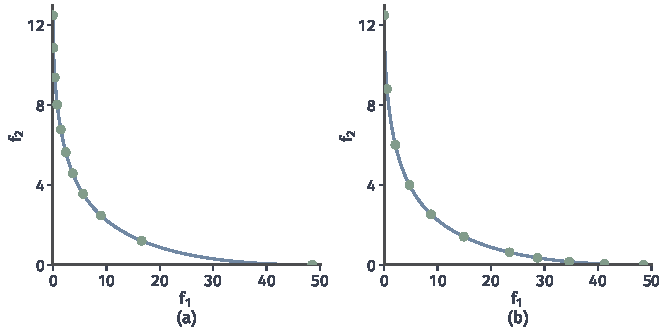
\includegraphics[width=112mm]{figures/05-optimization/07-multiple-criteria-and-nested-optimization/matplotlib/moo-scan-gaps/figure.pdf}
  \caption{例~\eqref{eq:moo-mgda-example}前沿上的$11$个候选。(a)$w$在$[0,1]$上均匀取值，点集中在左上方。(b)按最大空缺逐次补点，权重取空缺两端连线的法向。两图的端点相同。}
  \label{fig:moo-scan-gaps}
\end{BookInlineFigure}

\paragraph{按空缺补点}
既然均匀的参数靠不住，就让已经算出的点来决定下一个参数。对凸前沿，下面的过程很自然。

先用两个端点权重算出两端的点。然后反复做这样一步：找出归一化后间距最大的相邻两点$\bm{p},\bm{q}$，取这两点连线的法向作为新的权重，
\begin{equation}
 w=\frac{\lvert q_2-p_2\rvert}{\lvert q_2-p_2\rvert+\lvert q_1-p_1\rvert},
 \label{eq:moo-chord-weight}
\end{equation}
求解相应的加权和，把新点插进去。新权重下，支撑线与连线平行，解是这段前沿上离连线最远的点。若解不比$\bm{p},\bm{q}$的连线更靠左下，说明这一段已经没有新的支撑点，把这段标记为完成。

在例~\eqref{eq:moo-iso}上走几步。两端是$(0,1)$和$(1,0)$，由式~\eqref{eq:moo-chord-weight}得$w=1/2$，由式~\eqref{eq:moo-iso-weighted}得新点$(1/4,1/4)$。

在$(0,1)$与$(1/4,1/4)$之间，两个差值是$3/4$和$1/4$，权重为
\[
 w=\frac{3/4}{3/4+1/4}=\frac34,
\]
新点是$(1/16,9/16)$。在$(1/4,1/4)$与$(1,0)$之间，同理$w=1/4$，新点是$(9/16,1/16)$。五个点到此与均匀权重的结果相同，继续补点时，算法开始根据实际空缺分配求解次数。

在例~\eqref{eq:moo-mgda-example}上，按这种做法得到图~\ref{fig:moo-scan-gaps}(b)，归一化间距的最大值降到约$0.296$，最小值约为$0.111$，同样$11$次求解分布均匀得多。这里的选取规则只用到已算出的点，但法向的含义依赖目标尺度，所以要先说明归一化的参考范围。

\paragraph{用邻近问题的解作初值}
相邻参数的解通常相隔不远，这启发了用上一个解作下一个问题的初值，称为\term{热启动}（warm start）。图~\ref{fig:moo-warm-start}比较了两种做法：用梯度法解$39$个加权子问题，步长取该子问题的$1/L$，梯度范数降到$10^{-3}$为止。

\begin{BookInlineFigure}
  \centering
  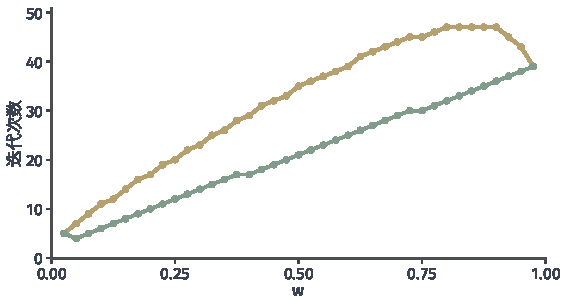
\includegraphics[width=96mm]{figures/05-optimization/07-multiple-criteria-and-nested-optimization/matplotlib/moo-warm-start/figure.pdf}
  \caption{例~\eqref{eq:moo-mgda-example}的$39$个加权子问题所用的梯度法迭代次数，$w$每步增加$0.025$。黄线是每次从$(0,2)$冷启动，共$1232$步；绿线是从上一个解热启动，共$826$步。}
  \label{fig:moo-warm-start}
\end{BookInlineFigure}

总迭代次数从$1232$降到$826$。线性收敛的方法从更好的初值出发，节省的是迭代次数对数中的一项，收敛速率本身不变，所以这里只节省三分之一左右，高精度要求下比例还会更小。

\paragraph{保存非支配候选}
扫描得到的点不一定都有用：求解可能不精确，并列解可能只是弱Pareto最优点。所以要维护一个\term{非支配存档}（non-dominated archive）。新点进来时，若被存档中的点支配就丢弃；否则把它支配的旧点删掉，再加入存档。

按$A,E,B,F,C,D$的顺序把式~\eqref{eq:moo-candidates}中的候选送入存档。$A$进入；$E$与$A$不可比，进入；$B$支配$E$，把$E$换成$B$；$F$与已有的点不可比，进入；$C$也进入；$D$支配$F$，把$F$换成$D$。最后得到$\{A,B,C,D\}$。

\paragraph{可达性的限制仍然存在}
无论参数取得多细，每种标量化能到达的点不会变多。图~\ref{fig:moo-scan-compare}在带凹陷的前沿上各取九个均匀的参数。加权和在$w\geq0.7$的三次求解全落到端点，凹陷段里一个点也没有，点从$(0.577,0.183)$直接跳到$(0.206,0.633)$。阈值约束和加权Chebyshev都把点放进了凹陷。

\begin{BookInlineFigure}
  \centering
  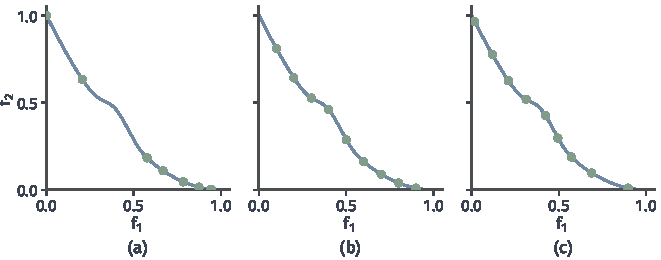
\includegraphics[width=112mm]{figures/05-optimization/07-multiple-criteria-and-nested-optimization/matplotlib/moo-scan-compare/figure.pdf}
  \caption{带凹陷的前沿上三种标量化的扫描，每种取九个均匀参数。(a)加权和，$w=0.1,\ldots,0.9$，$w\geq0.7$的三点重合在左端。(b)阈值约束，$\tau=0.1,\ldots,0.9$。(c)加权Chebyshev，$\bm{z}=(-0.1,-0.1)$，$\bm{w}=(w,1-w)$。}
  \label{fig:moo-scan-compare}
\end{BookInlineFigure}

所以，在非凸前沿上，要用阈值约束或加权Chebyshev来做扫描，并且每次求解都要检查是否达到全局最优。若子问题只解到局部最优，定理~\ref{thm:moo-threshold}和定理~\ref{thm:moo-chebyshev}的保证都不再适用。

\subsection{非支配排序}
\label{sec:moo-nsga}

参数扫描每次只优化一个点。能不能让一批候选同时朝前沿移动，并在前沿上散开？这一小节以NSGA-II为例，说明怎样把第~\ref{chap:random-search}章的种群搜索改造成服务前沿近似的算法。

\paragraph{主要思想}
\term{NSGA-II}（non-dominated sorting genetic algorithm II）沿用遗传算法的框架，维护一个规模为$N$的种群，变异和重组都与第~\ref{chap:random-search}章相同。要改造的是选择：单目标时按代价排序就能分出好坏，这里目标是向量，排序要回答两个问题。

第一个问题是谁离前沿更近。把种群按支配关系分层，不被任何个体支配的点是第一层；把第一层去掉后，剩下的点中不被支配的是第二层，依此类推。这个过程称为\term{非支配排序}（non-dominated sorting）。层号越小越靠近前沿。

第二个问题是同一层内谁应当保留。同一层的点互不支配，排不出优劣，但我们希望点在前沿上散开。所以优先保留周围比较空的点，用\term{拥挤距离}（crowding distance）度量。

对一层的点集，按目标$k$排序，设点$\bm{y}$的前后邻点为$\bm{y}^-$和$\bm{y}^+$，该层在目标$k$上的范围为$R_k$，拥挤距离是
\begin{equation}
 D(\bm{y})=\sum_{k=1}^m\frac{y_k^+-y_k^-}{R_k}.
 \label{eq:moo-crowding}
\end{equation}
每个目标上的两个端点取$D=\infty$，这样最大的和最小的值总被保留。式~\eqref{eq:moo-crowding}是以邻点为角的长方体的周长的一种度量。除以$R_k$使不同尺度的目标能够相加，也因此依赖该层的取值范围。

还有一个改造：下一代从亲代与后代的并集中选出，这就是\term{精英保留}（elitism）的做法，和第~\ref{chap:random-search}章的$(\mu+\lambda)$选择相同。好的亲代不会因后代变差而丢失。图~\ref{fig:moo-nsga-flow}是一代的流程。

\begin{BookInlineFigure}
  \centering
  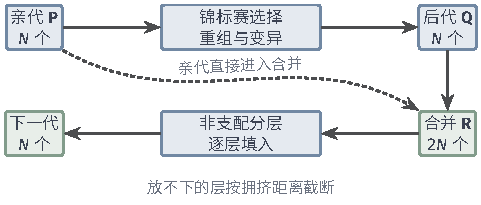
\includegraphics[width=81.5mm]{figures/05-optimization/07-multiple-criteria-and-nested-optimization/tikz/moo-nsga-flow/figure.pdf}
  \caption{NSGA-II的一代。亲代经锦标赛选择、重组与变异产生后代，亲代与后代合并成$2N$个候选，分层后逐层填入下一代，最后放不下的那一层按拥挤距离从大到小取。}
  \label{fig:moo-nsga-flow}
\end{BookInlineFigure}

\needspace{6\baselineskip}
\paragraph{变量}
\begin{itemize}
 \item 种群$\bm{P}$，$N$个候选及其目标向量，每个候选的层号与拥挤距离；
 \item 后代$\bm{Q}$，$N$个候选；合并的集合$\bm{R}=\bm{P}\cup\bm{Q}$；
 \item 分层计算中的辅助量：$S_{\bm{p}}$是$\bm{p}$支配的点集，$n_{\bm{p}}$是支配$\bm{p}$的点数。
\end{itemize}

\paragraph{初始化}
随机产生$N$个候选并评价，分层并计算拥挤距离。下面用例子说明一代中的选择。假设合并后得到八个候选，它们是式~\eqref{eq:moo-candidates}的六个点，加上
\[
 G=(3,7),\qquad H=(6,7).
\]

\needspace{6\baselineskip}
\paragraph{每轮更新}
\begin{enumerate}
 \item 产生后代：用二元锦标赛选亲代，比较时层号小者胜，层号相同时拥挤距离大者胜；再做重组和变异。例中假定后代已经产生并合并。

 \item 合并亲代和后代，对每一点计算$n_{\bm{p}}$和$S_{\bm{p}}$。例中
 \[
  n_A=n_B=n_C=n_D=0,\quad n_E=2,\quad n_F=n_G=1,\quad n_H=5.
 \]
 $E$被$B,C$支配，$F$被$D$支配，$G$被$B$支配，$H$被$B,C,D,E,G$支配。

 \item 分层：$n_{\bm{p}}=0$的点组成第一层，把它们支配的点的$n$减一，$n$减到零的点组成下一层，依此类推。例中第一层是$\{A,B,C,D\}$。把它们去掉后$n_E=n_G=n_F=0$，第二层是$\{E,F,G\}$，第三层是$\{H\}$，见图~\ref{fig:moo-nsga-layers}(a)。

 \item 逐层填入下一代，直到某一层放不下。例中取$N=6$，第一层四个点全部进入，还差两个名额。

 \item 放不下的那一层，计算拥挤距离~\eqref{eq:moo-crowding}，按从大到小取够。例中第二层$G,E,F$按$f_1$排序是$G,E,F$，$G,F$是端点，距离为无穷；$E$的距离是
 \[
  D(E)=\frac{7-3}{7-3}+\frac{7-1}{7-1}=2.
 \]
 所以取$G$和$F$，$E$被淘汰。下一代是$\{A,B,C,D,F,G\}$。
\end{enumerate}

这一例也提醒我们，$F$虽然只是弱Pareto最优点，却因为端点的身份进入了下一代。分层只反映种群内部的关系。

截断也可能发生在第一层。若$N=3$，第一层四个点要留三个。$A$和$D$是端点，距离为无穷。其余两点的距离由式~\eqref{eq:moo-crowding}算出：
\[
 D(B)=\frac{4-1}{5}+\frac{8-4}{7}\approx1.171,\qquad
 D(C)=\frac{6-2}{5}+\frac{5-1}{7}\approx1.371.
\]
所以保留$A,C,D$，淘汰$B$，图~\ref{fig:moo-nsga-layers}(b)画出了这两个长方形。$C$在加权和下永远选不上，在这里却因为不拥挤而被留下：种群搜索的比较只用支配和距离，不要求支撑。

\begin{BookInlineFigure}
  \centering
  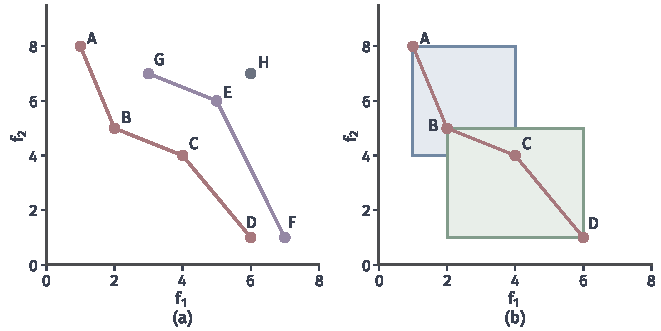
\includegraphics[width=112mm]{figures/05-optimization/07-multiple-criteria-and-nested-optimization/matplotlib/moo-nsga-layers/figure.pdf}
  \caption{八个候选的非支配排序与拥挤距离。(a)红色、紫色、灰色依次是第一、二、三层。(b)第一层内$B$与$C$的拥挤长方形，分别以$A,C$和$B,D$为角，$C$的长方形更大。}
  \label{fig:moo-nsga-layers}
\end{BookInlineFigure}

\paragraph{运行效果}
一代中比较支配关系的开销是$O(mN^2)$，拥挤距离的排序是$O(mN\log N)$，加上$N$次目标评价。目标评价昂贵时，主要开销是评价的次数。

图~\ref{fig:moo-nsga-run}是在一个五维问题上的实际运行。取$\bm{x}\in[0,1]^5$，
\begin{equation}
 f_1=x_1,\quad \gamma=1+\frac{9}{4}\sum_{j=2}^{5}x_j,\quad f_2=\gamma\Bigl(1-\bigl(f_1/\gamma\bigr)^2\Bigr).
 \label{eq:moo-zdt}
\end{equation}
当$x_2=\cdots=x_5=0$时$\gamma=1$，$f_2=1-f_1^2$，这就是式~\eqref{eq:moo-concave}的抛物线前沿。其余变量把点往上推。种群规模为$40$，运行$200$代，随机种子固定。

\begin{BookInlineFigure}
  \centering
  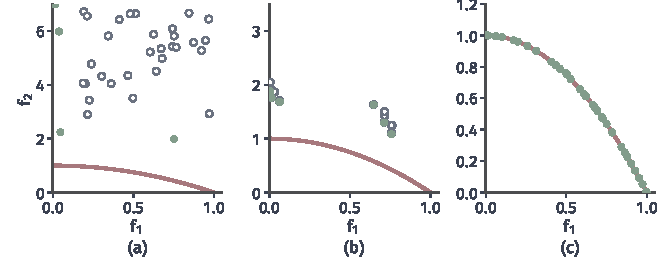
\includegraphics[width=112mm]{figures/05-optimization/07-multiple-criteria-and-nested-optimization/matplotlib/moo-nsga-run/figure.pdf}
  \caption{NSGA-II在式~\eqref{eq:moo-zdt}上的种群，种群规模$40$。红线是真实前沿，绿点是当前种群的第一层，空心点是其余个体。(a)初始种群。(b)第$10$代，第一层有$12$个点，互不支配，但离前沿还很远。(c)第$200$代，$40$个点都在前沿附近。三幅图的纵轴范围不同。}
  \label{fig:moo-nsga-run}
\end{BookInlineFigure}

第$10$代的$12$个点互不支配，却离真实前沿还很远。这正是必须记住的一点：有限种群内部互不支配，不能说明它们是Pareto最优的。算法没有全局保证，它的结果要靠第~\ref{sec:moo-front-evaluation}节的量来检查。加权和扫描在这个问题上只能得到两个端点，这里的种群搜索能把点散布到整条前沿上，这是它的优势。

\section{前沿的评价}
\label{sec:moo-front-evaluation}

算法交出了一组候选，这组候选好不好？真实前沿通常是未知的，所以要明确：在固定目标尺度和计算预算的情况下，能报告哪些可计算的量，它们分别说明什么。本节先看单个候选的质量，再看整组候选的覆盖范围。

\subsection{候选质量}
\label{sec:moo-candidate-quality}

一个候选点要检查什么？这一小节列出三项检查：是否可行，它自己的子问题解得好不好，以及是否还有共同下降的余地。

\paragraph{约束违反}
第一项是可行性。对每个候选报告最大约束违反量
\begin{equation}
 \mathrm{viol}(\bm{x})=\max\Bigl\{\max_j\,[g_j(\bm{x})]_+,\ \max_k\,\lvert h_k(\bm{x})\rvert\Bigr\},
 \label{eq:moo-violation}
\end{equation}
其中$[v]_+=\max\{v,0\}$。违反约束的点不能参与支配比较：稍微违反约束的点常常看起来更好，让它留在候选集中，会把真正可行的点错误地淘汰掉。

\paragraph{两种残差}
第二项是该候选作为优化结果的误差，这要看它是怎么得来的，要回答的问题也不同。

若候选来自权重$\bm{w}$的无约束加权和，就看它作为这个单目标问题的解有多准，用\term{标量子问题误差}（scalar subproblem error）衡量，光滑无约束时常用梯度范数
\begin{equation}
 \rho_{\bm{w}}(\bm{x})=\Bigl\lVert\sum_{i=1}^mw_i\nabla f_i(\bm{x})\Bigr\rVert_2.
 \label{eq:moo-scalar-residual}
\end{equation}

若候选是作为Pareto驻定点提交的，要看的是\term{共同下降残差}（common descent residual）$\lVert\bar{\bm{g}}(\bm{x})\rVert_2$，也就是式~\eqref{eq:moo-min-norm}中的最短长度。

这两种残差回答的问题不同。由于$\bar{\bm{g}}$是所有凸组合中最短的，对任意$\bm{w}\in\Delta_m$，
\begin{equation}
 \lVert\bar{\bm{g}}(\bm{x})\rVert_2\leq\rho_{\bm{w}}(\bm{x}).
 \label{eq:moo-residual-order}
\end{equation}
标量残差小，共同下降残差必定也小；反过来不成立。

在例~\eqref{eq:moo-iso}上算两个候选，权重都取$(1/2,1/2)$。第一个候选$\hat{\bm{x}}=(0.9,0.1)$在解集上，
\[
 \bm{g}_1=(-0.1,0.1),\qquad\bm{g}_2=(0.9,-0.9).
\]
两个梯度反向，$\lVert\bar{\bm{g}}\rVert_2=0$，它是驻定的。但
\[
 \rho_{\bm{w}}=\lVert(0.4,-0.4)\rVert_2\approx0.566.
\]
所以这个点是前沿上的一点，却不是“两项同样重要”这个偏好下的解。

第二个候选$\hat{\bm{x}}=(0.6,0.5)$略微偏离解集，
\[
 \bm{g}_1=(-0.4,0.5),\qquad\bm{g}_2=(0.6,-0.5).
\]
由式~\eqref{eq:moo-theta-two}算出$\theta^\star=0.55$，$\bar{\bm{g}}=(0.05,0.05)$，其长度约为$0.071$；而$\rho_{\bm{w}}=\lVert(0.1,0)\rVert_2=0.1$。两个残差都不为零，式~\eqref{eq:moo-residual-order}成立。

图~\ref{fig:moo-candidate-residual}把这种差别沿着整条线段画了出来：解集上共同下降残差处处为零，标量残差却只在$s=1/2$处为零。偏离解集的距离加入后，两种残差都不再为零。所以报告残差时要说清楚是哪一种。若目的是“实现这个偏好”，就看$\rho_{\bm{w}}$；若目的是“候选不能再被一阶共同改进”，就看$\lVert\bar{\bm{g}}\rVert_2$。

\begin{BookInlineFigure}
  \centering
  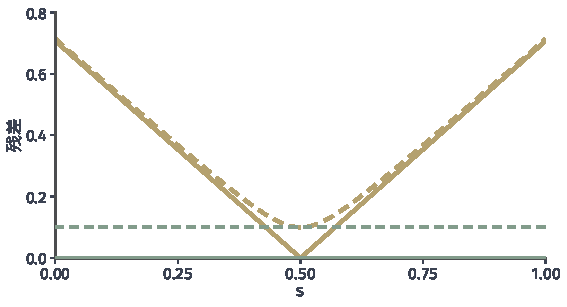
\includegraphics[width=96mm]{figures/05-optimization/07-multiple-criteria-and-nested-optimization/matplotlib/moo-candidate-residual/figure.pdf}
  \caption{例~\eqref{eq:moo-iso}中两种残差沿$\bm{x}(s)=(1-s,s)+\delta(1,1)/\sqrt2$的变化。绿线是共同下降残差，黄线是$\bm{w}=(1/2,1/2)$的标量残差，实线为$\delta=0$，虚线为$\delta=0.1$。}
  \label{fig:moo-candidate-residual}
\end{BookInlineFigure}

约束问题中，$\rho_{\bm{w}}$和$\lVert\bar{\bm{g}}\rVert_2$要换成相应的KKT残差，即式~\eqref{eq:moo-kkt}的左端在给定乘子下的范数，再加上互补松弛的误差。

\paragraph{筛选的局限}
第三项是把候选集中被支配的点剔除，用第~\ref{sec:moo-scan}节的存档方法即可。剔除之后剩下的点互不支配，但这只是在已有候选之间比较。

图~\ref{fig:moo-hidden-dominator}中，$A,B,C,D$互不支配。如果有一个没被算到的方案$\bm{P}=(3,3)$，它支配$C$，粉色区域中的方案都比它差。有限候选之间的筛选，永远不能证明不存在尚未找到的支配方案。

\begin{BookInlineFigure}
  \centering
  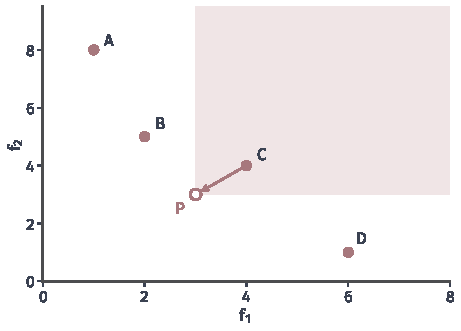
\includegraphics[width=78mm]{figures/05-optimization/07-multiple-criteria-and-nested-optimization/matplotlib/moo-hidden-dominator/figure.pdf}
  \caption{有限候选的筛选不足以判定最优。红点$A,B,C,D$互不支配，尚未找到的方案$\bm{P}=(3,3)$（红色空心点）却支配$C$，$C$落在$\bm{P}$的被支配区域（粉色）中。}
  \label{fig:moo-hidden-dominator}
\end{BookInlineFigure}

证明一个候选是全局Pareto最优的办法有两种：问题是凸的，用定理~\ref{thm:moo-kkt-sufficient}；或者全局求解一个能够选中它的标量子问题。两种都不能依靠候选之间的比较。

\subsection{覆盖范围}
\label{sec:moo-coverage}

单个候选合格，整组未必合格，它们可能都挤在前沿的一小段上。这一小节讨论怎样用数字描述整组候选的质量，以及每个数字的局限。

\paragraph{超体积}
取一个比所有候选都差的\term{参考点}$\bm{r}$，也就是各分量都大于候选相应分量的点。候选集$\bm{S}$支配的、并被$\bm{r}$界住的区域的体积称为\term{超体积}（hypervolume）：
\begin{equation}
 \mathrm{HV}(\bm{S};\bm{r})=\mathrm{vol}\Bigl(\bigcup_{\bm{y}\in\bm{S}}\{\bm{z}:\bm{y}\leq\bm{z}\leq\bm{r}\}\Bigr).
 \label{eq:moo-hv}
\end{equation}
一个指标把“离前沿多近”和“覆盖多宽”都包含进来：候选越靠前沿，被支配区域越大；候选越分散，并集越大。

两个目标时超体积可以按条带求和。把候选按$f_1$从小到大排序，设互不支配，记第$i$点为$(y_{1,i},y_{2,i})$，$i=1,\ldots,N$，并约定$y_{1,N+1}=r_1$。则
\begin{equation}
 \mathrm{HV}=\sum_{i=1}^{N}(y_{1,i+1}-y_{1,i})(r_2-y_{2,i}).
 \label{eq:moo-hv-2d}
\end{equation}

对$A,B,C,D$取$\bm{r}=(8,9)$，四个条带的面积是
\[
 (2-1)(9-8)=1,\quad(4-2)(9-5)=8,\quad(6-4)(9-4)=10,\quad(8-6)(9-1)=16,
\]
总和$\mathrm{HV}=35$，见图~\ref{fig:moo-hypervolume}。把$E$或$F$加进来，超体积不变，因为它们支配的区域已经被覆盖。把$C$去掉，超体积变成$33$，$C$独占的贡献是$(6-4)(5-4)=2$。

\begin{BookInlineFigure}
  \centering
  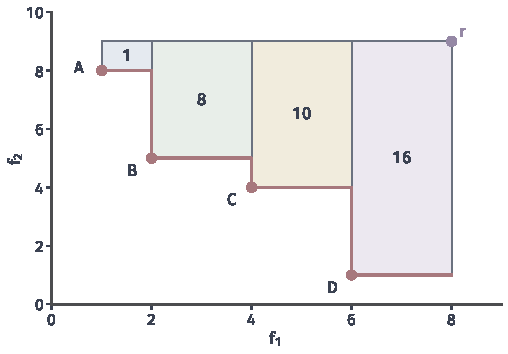
\includegraphics[width=86mm]{figures/05-optimization/07-multiple-criteria-and-nested-optimization/matplotlib/moo-hypervolume/figure.pdf}
  \caption{$A,B,C,D$的超体积，参考点$\bm{r}=(8,9)$。彩色条带的面积分别是$1,8,10,16$，合计$35$。红色阶梯线是这组候选支配区域的左下边界。}
  \label{fig:moo-hypervolume}
\end{BookInlineFigure}

超体积的好处在于它和支配关系是相容的。

\begin{theorem}[超体积的单调性]
\label{thm:moo-hv-monotone}
设$\bm{S},\bm{S}'$的所有点都逐分量不大于$\bm{r}$。若对每个$\bm{y}'\in\bm{S}'$，存在$\bm{y}\in\bm{S}$使$\bm{y}\leq\bm{y}'$，则
\begin{equation}
 \mathrm{HV}(\bm{S};\bm{r})\geq\mathrm{HV}(\bm{S}';\bm{r}).
 \label{eq:moo-hv-monotone}
\end{equation}
\end{theorem}

\begin{proof}
若$\bm{y}\leq\bm{y}'\leq\bm{z}\leq\bm{r}$，则$\bm{y}\leq\bm{z}\leq\bm{r}$。所以$\bm{S}'$对应的并集包含在$\bm{S}$对应的并集中，体积不减。
\end{proof}

也就是说，把一组候选换成支配它们的另一组，超体积不会下降。

\paragraph{参考点和尺度}
超体积不是一个自足的数字，它依赖参考点。设$\bm{S}_1=\{(1,6),(6,1)\}$，$\bm{S}_2=\{(3,3)\}$。取$\bm{r}=(7,7)$，由式~\eqref{eq:moo-hv-2d}，
\[
 \mathrm{HV}(\bm{S}_1)=5\times1+1\times6=11,\qquad\mathrm{HV}(\bm{S}_2)=4\times4=16.
\]
$\bm{S}_2$更好。取$\bm{r}=(20,20)$，
\[
 \mathrm{HV}(\bm{S}_1)=5\times14+14\times19=336,\qquad\mathrm{HV}(\bm{S}_2)=17\times17=289.
\]
$\bm{S}_1$更好。参考点越远，越看重前沿的两端，见图~\ref{fig:moo-hv-reference}。比较不同算法时，参考点必须事先固定，并且和结果一起报告。

\begin{BookInlineFigure}
  \centering
  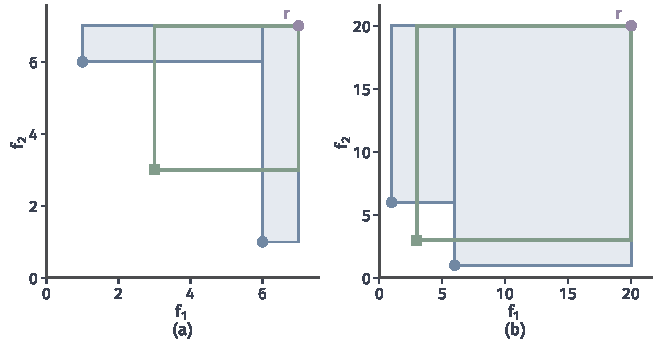
\includegraphics[width=112mm]{figures/05-optimization/07-multiple-criteria-and-nested-optimization/matplotlib/moo-hv-reference/figure.pdf}
  \caption{超体积比较依赖参考点。蓝色区域属于$\bm{S}_1=\{(1,6),(6,1)\}$，绿色方框属于$\bm{S}_2=\{(3,3)\}$。(a)$\bm{r}=(7,7)$，$\bm{S}_2$较大。(b)$\bm{r}=(20,20)$，$\bm{S}_1$较大。}
  \label{fig:moo-hv-reference}
\end{BookInlineFigure}

尺度的影响也要说明。把目标$k$乘以$c>0$，参考点相应乘以$c$，所有超体积同乘$c$，比较结果不变。但把目标归一化时，若参考范围随候选集而变，每组候选用的就是不同的尺子，比较便失去了共同的基准。

\paragraph{空缺与取舍范围}
超体积把很多信息压成一个数，可能掩盖分布上的差别。还要报告相邻候选之间的最大间距和目标的取舍范围。

在例~\eqref{eq:moo-iso}的前沿上，用$s$值表示候选，取$\bm{S}_1:\ s=0.1,0.5,0.9$与$\bm{S}_2:\ s=0.24,0.515,0.975$。取$\bm{r}=(1.2,1.2)$，两者的超体积都等于$1.0897$，见图~\ref{fig:moo-coverage-distance}。可是把前沿两端也算上，$\bm{S}_1$的最大相邻间距约为$0.609$，$\bm{S}_2$约为$0.724$，$\bm{S}_2$在靠$f_2$轴的一端空出了更大的一段。

\begin{BookInlineFigure}
  \centering
  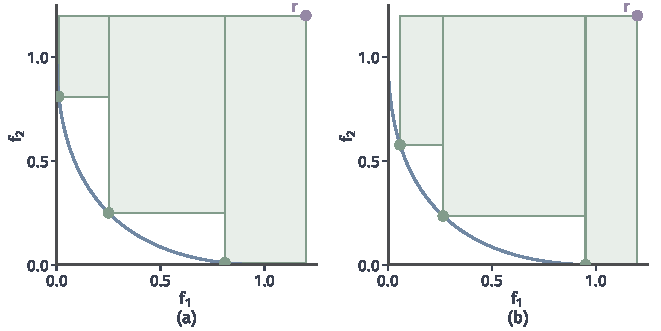
\includegraphics[width=112mm]{figures/05-optimization/07-multiple-criteria-and-nested-optimization/matplotlib/moo-coverage-distance/figure.pdf}
  \caption{两组超体积相同（$\bm{r}=(1.2,1.2)$，$\mathrm{HV}=1.0897$）的候选，蓝线是真实前沿。(a)$s=0.1,0.5,0.9$。(b)$s=0.24,0.515,0.975$，最大相邻间距更大。}
  \label{fig:moo-coverage-distance}
\end{BookInlineFigure}

\paragraph{到参考前沿的距离}
若有可信的参考前沿$\bm{R}$，比如问题有解析解，或者是长时间计算汇总的结果，可以进一步计算候选集与它的距离。两个常用的量是\term{世代距离}（generational distance，GD）和\term{反向世代距离}（inverted generational distance，IGD）：
\begin{equation}
 \begin{aligned}
  \mathrm{GD}&=\frac{1}{\lvert\bm{S}\rvert}\sum_{\bm{y}\in\bm{S}}\min_{\bm{p}\in\bm{R}}\lVert\bm{y}-\bm{p}\rVert_2,\\
  \mathrm{IGD}&=\frac{1}{\lvert\bm{R}\rvert}\sum_{\bm{p}\in\bm{R}}\min_{\bm{y}\in\bm{S}}\lVert\bm{y}-\bm{p}\rVert_2.
 \end{aligned}
 \label{eq:moo-gd-igd}
\end{equation}

GD看候选离前沿有多近，IGD看前沿被候选覆盖得多好。图~\ref{fig:moo-coverage-distance}的两组候选都在前沿上，GD都是零。IGD用$1001$个参考点计算，$\bm{S}_1$约为$0.143$，$\bm{S}_2$约为$0.163$，这里区分出了两组候选的覆盖差别。

这些量都要有参考前沿才能算。若参考前沿是其他算法的结果，算出的就只是相对的差别，不是真实误差。

\paragraph{多个指标一起看}
图~\ref{fig:moo-nsga-indicators}是图~\ref{fig:moo-nsga-run}那次运行的指标曲线，参考点取$\bm{r}=(1.1,1.1)$。超体积在第$40$代已经到$0.512$，真实前沿对应的值是$0.5433$，第$200$代是$0.5245$。到参考前沿的平均距离第$100$代约为$0.0141$，第$200$代约为$0.0153$，并不单调。

\begin{BookInlineFigure}
  \centering
  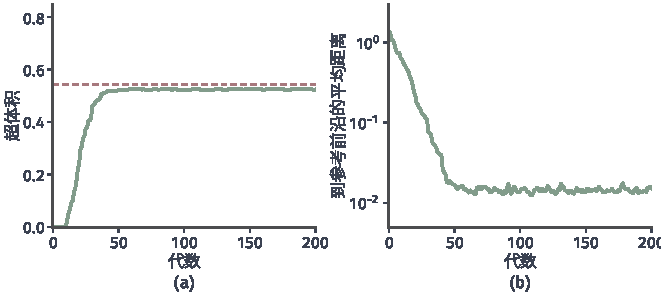
\includegraphics[width=112mm]{figures/05-optimization/07-multiple-criteria-and-nested-optimization/matplotlib/moo-nsga-indicators/figure.pdf}
  \caption{NSGA-II运行中的指标，问题为式~\eqref{eq:moo-zdt}。(a)超体积，$\bm{r}=(1.1,1.1)$，红色虚线是真实前沿的值$0.5433$。(b)种群第一层到参考前沿的IGD，纵轴为对数。曲线后段不是单调的。}
  \label{fig:moo-nsga-indicators}
\end{BookInlineFigure}

种群只有$40$个点，覆盖不了整条曲线，超体积不会达到$0.5433$，这个差额来自有限的点数。同一种群的第一层不断变化时，IGD也可以上下波动。不能用一个集合指标代替所有判断。表~\ref{tab:moo-indicators}列出各个量各自回答的问题。

\begin{BookInlineTable}
  \centering
  \caption{候选集的常用评价量。}
  \label{tab:moo-indicators}
  \begin{tabular}{@{}lll@{}}
    \toprule
    量 & 回答的问题 & 需要的条件\\
    \midrule
    约束违反 & 是否可行 & 约束函数\\
    标量残差 & 这次偏好解得准不准 & 权重或阈值\\
    共同下降残差 & 还能否一阶共同改进 & 梯度\\
    超体积 & 支配区域多大 & 固定的$\bm{r}$与尺度\\
    最大间距 & 前沿上有无大空缺 & 目标尺度\\
    GD与IGD & 离参考前沿多近 & 可信的参考前沿\\
    \bottomrule
  \end{tabular}
\end{BookInlineTable}

把这些量都算出来，能说的话仍然有限：这组候选满足约束，单点的残差如此，在这个参考点下超体积如此。不能说“已经恢复了完整的Pareto前沿”，除非另有理论保证。

\section{本章小结}
\label{sec:moo-summary}

本章从“两个目标各有所长的方案谁更好”出发。结论是，不依赖偏好的比较只有支配关系，由它得到的是一组互不支配的方案，而不是一个方案。目标冲突不会因为单目标算法更强而消失，强的算法只能更快地解出某一个偏好下的问题。

支配关系是第一层判断，它不受单位影响。权重、距离和归一化都依赖尺度，使用时要写明单位与参考范围。

偏好由三种标量化表达。加权和相当于定价，权重全正的全局解是Pareto最优的，凸问题中非负权重足以选中每个弱Pareto最优点，但在非凸前沿上会遗漏非支撑点。阈值约束相当于定预算，加权Chebyshev相当于要求各项接近某个水平，二者不需要凸性就能选中每个Pareto点，但可能返回并列的弱Pareto最优解，需要第二阶段的择优。

局部信息给出一阶判别。Pareto驻定说明不存在严格共同下降的方向，这是局部弱Pareto最优的必要条件，有约束时要在约束资格下配合乘子；要由它推出全局结论，还需要凸性，权重全正时才能得到Pareto最优。多梯度下降从梯度凸包的最小范数元得到共同下降方向，配合共同步长使每个目标都下降，一次运行收敛到一个驻定点。

要得到一组候选，可以扫描偏好参数，用热启动降低代价，按空缺补点，并用非支配存档保存结果；也可以用NSGA-II这样的群体搜索，以分层和拥挤距离代替单目标的排序。两者都要在固定的目标尺度下，用约束违反、残差、超体积、间距以及到参考前沿的距离来检查。

图~\ref{fig:moo-summary}汇总了四种结果之间的关系。加权最优、Pareto驻定、全局Pareto最优和有限候选集的覆盖是四种不同的结论，从一种到另一种都需要说明所依赖的条件。

\begin{BookInlineFigure}
  \centering
  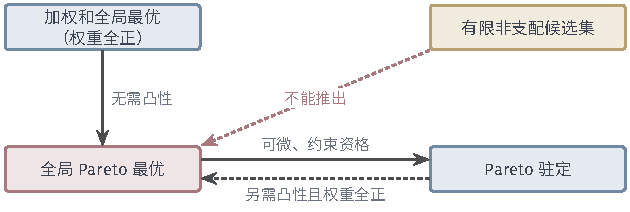
\includegraphics[width=106.7mm]{figures/05-optimization/07-multiple-criteria-and-nested-optimization/tikz/moo-summary/figure.pdf}
  \caption{四种结果的关系。实线箭头在标注的条件下成立，虚线箭头需要额外的条件，红色虚线表示有限候选集互不支配不能推出全局Pareto最优。}
  \label{fig:moo-summary}
\end{BookInlineFigure}


\chapter{极小极大优化}
\label{chap:minimax-optimization}

一个设定值$x$定下来之后，实际需求$y$还会在$[-1,1]$内变动，偏差的代价是$(x-y)^2$。如果要求方案在允许范围内最坏的情形下也过得去，$x$该怎样选？取$x=0.5$，最坏的需求是$y=-1$，代价是$2.25$；取$x=0$，最坏的代价是$1$。评价一个方案不再是算一个函数值，而是要先解一个最大化问题。

这类问题的外层要让代价小，内层要让同一个代价大。两层方向相反，带来三个单目标问题里没有的困难：先选谁会改变答案；内层最优的$y$随$x$切换，外层目标因此可能没有导数；两组变量一起迭代时，轨迹可能绕着解打转而不靠近它。

第~\ref{sec:minimax-problem}节把决策顺序写成准确的数学问题。第~\ref{sec:minimax-value-function}节把内层收进一个只依赖$\bm{x}$的函数，研究它何时有意义、何时可微。第~\ref{sec:minimax-saddle}节回答两个次序何时给出同一个值，并给出检验一对候选的数值证书。

求解有两条路线。第~\ref{sec:minimax-inner-response}节沿决策顺序先求内层响应，再更新外层。第~\ref{sec:minimax-gda}节和第~\ref{sec:minimax-correction}节让两组变量同时走，先看最直接的做法为什么会失败，再用校正方向修复。第~\ref{sec:minimax-evaluation}节说明算完之后拿什么证据判断结果的好坏。

\section{极小极大问题}
\label{sec:minimax-problem}

“先定方案，再承受最坏的响应”，怎样写成一个含义准确的优化问题？

设$\bm{X}\subseteq\mathbb{R}^{n}$，$\bm{Y}\subseteq\mathbb{R}^{q}$是预先给定、互不依赖的非空集合，$f:\bm{X}\times\bm{Y}\to\mathbb{R}$是代价。$\bm{x}$是方案，$\bm{y}$是允许的响应。我们研究
\begin{equation}
 \inf_{\bm{x}\in\bm{X}}\ \sup_{\bm{y}\in\bm{Y}}\ f(\bm{x},\bm{y}),
 \label{eq:minimax-problem}
\end{equation}
称为\term{极小极大问题}（minimax problem）。这个式子要从里往外读：对每个固定的$\bm{x}$，内层求$\bm{x}$所能遭遇的最坏代价；外层在所有方案中选最坏代价最小的那个。

内层面对的是一个已经选定的$\bm{x}$，它不是一个可以脱离外层单独解出来的优化问题。在开头的例子里，$x=0.5$时最坏的$y$是$-1$，$x=-0.5$时最坏的$y$是$1$。单独问“最坏的$y$是什么”没有答案，内层实际上是一族问题，每个$\bm{x}$对应一个。

把内层的$\sup$换成$\inf$，情况完全不同。两层都最小化时，
\[
 \inf_{\bm{x}\in\bm{X}}\inf_{\bm{y}\in\bm{Y}}f(\bm{x},\bm{y})=\inf_{(\bm{x},\bm{y})\in\bm{X}\times\bm{Y}}f(\bm{x},\bm{y}),
\]
两层可以合并成一个联合最小化，这正是第~\ref{chap:block-optimization}章能够交替更新各块的前提。极小极大问题做不到这一点，一个变量要下山，另一个变量要上山，没有一个共同的目标能把两者合起来。

\subsection{响应顺序}
\label{sec:minimax-order}

先用一张有限的代价表看次序的作用。有两个方案$\mathrm{a},\mathrm{b}$和两种扰动，代价如图~\ref{fig:minimax-cost-table}所示。

\begin{BookInlineFigure}
 \centering
 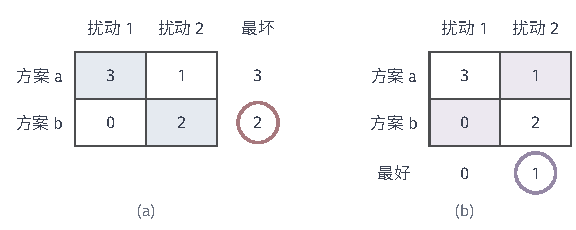
\includegraphics[width=97.5mm]{figures/05-optimization/07-multiple-criteria-and-nested-optimization/tikz/minimax-cost-table/figure.pdf}
 \caption{同一张代价表，两种决策顺序。(a)先定方案：每行取最大（蓝底），最坏列在表右，再在两个最坏值中取小，得到红圈中的$2$。(b)先定扰动：每列取最小（紫底），最好列在表下，再在两个最好值中取大，得到紫圈中的$1$。}
 \label{fig:minimax-cost-table}
\end{BookInlineFigure}

先定方案、再来扰动时，方案$\mathrm{a}$的最坏代价是$3$，方案$\mathrm{b}$的最坏代价是$2$，所以选$\mathrm{b}$，代价是$2$。这就是式~\eqref{eq:minimax-problem}的次序。

反过来，先定扰动、再选方案时，扰动$1$下最好的方案代价是$0$，扰动$2$下最好的方案代价是$1$。扰动一方要让代价大，所以选扰动$2$，代价是$1$。两个次序写成
\[
 \min_{\text{方案}}\max_{\text{扰动}}=2,\qquad\max_{\text{扰动}}\min_{\text{方案}}=1.
\]

同一张表给出两个不同的数。差别来自信息：后选的一方看得到先选的一方，可以对症下药。选方案的一方后选时代价是$1$，先选时代价是$2$，多出来的$1$是先亮底牌的代价。

后选不吃亏这件事不依赖具体的表。

\begin{lemma}[弱极小极大不等式]
\label{lem:minimax-weak}
对任意非空集合$\bm{X},\bm{Y}$和任意$f:\bm{X}\times\bm{Y}\to\mathbb{R}$，
\begin{equation}
 \sup_{\bm{y}\in\bm{Y}}\inf_{\bm{x}\in\bm{X}}f(\bm{x},\bm{y})\leq\inf_{\bm{x}\in\bm{X}}\sup_{\bm{y}\in\bm{Y}}f(\bm{x},\bm{y}).
 \label{eq:minimax-weak}
\end{equation}
\end{lemma}

\begin{proof}
任取$\bm{x}'\in\bm{X}$和$\bm{y}'\in\bm{Y}$。下确界不超过其中任何一项，上确界不小于其中任何一项，所以
\[
 \inf_{\bm{x}\in\bm{X}}f(\bm{x},\bm{y}')\leq f(\bm{x}',\bm{y}')\leq\sup_{\bm{y}\in\bm{Y}}f(\bm{x}',\bm{y}).
\]
最左端不含$\bm{x}'$，最右端不含$\bm{y}'$。左端对$\bm{y}'$取上确界，右端对$\bm{x}'$取下确界，不等号保持。
\end{proof}

连续的例子也一样。回到开头的$f(x,y)=(x-y)^2$，$X=\mathbb{R}$，$Y=[-1,1]$。固定$x$时，$f$是$y$的凸函数，最大值在端点取到，所以
\[
 \sup_{y\in[-1,1]}(x-y)^2=\max\{(x+1)^2,(x-1)^2\}=(\lvert x\rvert+1)^2.
\]

上式在$x=0$处最小，于是先定方案的值是$1$。反过来，无论$y$是多少，后选的$x$都可以取$x=y$，使代价为零，所以先定扰动的值是$0$。图~\ref{fig:minimax-worst-envelope}(a)里，外层最小化的是粗蓝线，而不是任何一条细线。

\begin{BookInlineFigure}
 \centering
 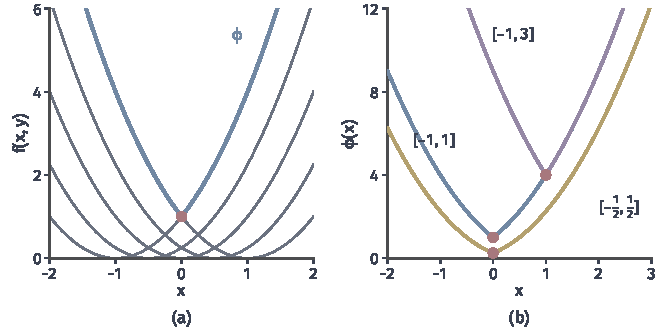
\includegraphics[width=112mm]{figures/05-optimization/07-multiple-criteria-and-nested-optimization/matplotlib/minimax-worst-envelope/figure.pdf}
 \caption{$f(x,y)=(x-y)^2$的最坏代价。(a)灰线是$y=0,\pm\frac12,\pm1$时的$f(\cdot,y)$，蓝线是它们对全部$y\in[-1,1]$的上边缘$\phi(x)=(\lvert x\rvert+1)^2$，红点是外层最优解。(b)三种响应集合下的最坏代价，黄线、蓝线、紫线分别对应标注的集合，红点是各自的最优解。集合$[-1,3]$把最优解移到了$x=1$。}
 \label{fig:minimax-worst-envelope}
\end{BookInlineFigure}

式~\eqref{eq:minimax-weak}的等号一般不成立，上面两个例子都严格小于。所以式~\eqref{eq:minimax-problem}里$\inf$和$\sup$的次序是问题的一部分，不能随手交换。交换需要额外的条件，第~\ref{sec:minimax-saddle}节专门研究。

\subsection{模型边界}
\label{sec:minimax-boundary}

极小极大的结论只对写进模型的$\bm{Y}$负责。“最坏”指的是集合$\bm{Y}$里最坏，集合之外的情形不在保证之内。

图~\ref{fig:minimax-worst-envelope}(b)比较了三个响应集合。对对称的集合$[-\rho,\rho]$，同样的计算给出最坏代价$(\lvert x\rvert+\rho)^2$，最优解都是$x=0$，最优值是$\rho^2$。集合放大时值变大，解却碰巧没动，这很容易让人以为解不依赖集合。

换成不对称的$Y=[-1,3]$，最坏代价变成
\[
 \max\{(x+1)^2,(x-3)^2\}.
\]
两条抛物线在$x=1$相交，最优解是$x=1$，最优值是$4$。按$Y=[-1,1]$选出的$x=0$，放到这个更大的集合下，最坏代价是$(0-3)^2=9$，比$4$差很多。一般地，$\bm{Y}_1\subseteq\bm{Y}_2$时内层上确界只会变大，所以小集合上的最坏值只是大集合上最坏值的下界，小集合上的最优解在大集合上没有任何保证。

\paragraph{Lagrange鞍点是特例}
第~\ref{chap:duality}章已经见过这种结构。约束问题的Lagrange函数$\mathcal{L}$对乘子取上确界时，可行点得到$f(\bm{x})$，不可行点得到$+\infty$，原问题因此写成
\[
 \inf_{\bm{x}\in\bm{D}}\ \sup_{\bm{\lambda}\geq\bm{0},\,\bm{\nu}}\ \mathcal{L}(\bm{x},\bm{\lambda},\bm{\nu}).
\]

这相当于在式~\eqref{eq:minimax-problem}中取$\bm{y}=(\bm{\lambda},\bm{\nu})$，$\bm{Y}=\mathbb{R}^m_{+}\times\mathbb{R}^p$，$\bm{X}=\bm{D}$。对偶问题是交换次序后的$\sup\inf$，弱对偶就是式~\eqref{eq:minimax-weak}。这个特例的结构比一般情形简单，$\mathcal{L}$关于$\bm{y}$是线性的，并且$\bm{Y}$由符号约束给出。本章的$f$不必有这种结构，$\bm{Y}$也可以是任意给定的集合。

\paragraph{本章不讨论的内容}
本章只有一个固定的代价$f$，$\bm{y}$只是“允许的响应”这个数学对象，不代表一个有自身偏好的决策者。模型中各方的偏好、均衡的解释和随时间展开的策略属于另一类问题，可参考\BookChapterRef{chap:static-games-equilibrium}{卷十第8章“静态博弈与均衡”}。这里只研究静态问题~\eqref{eq:minimax-problem}及其数值求解。

\section{最坏值函数}
\label{sec:minimax-value-function}

外层真正面对的目标是什么？本节把内层收进一个只依赖$\bm{x}$的函数，然后研究这个函数的性质，因为外层能用什么算法，全由这些性质决定。

\begin{definition}[最坏值函数]
\label{def:minimax-value}
称
\begin{equation}
 \phi(\bm{x})=\sup_{\bm{y}\in\bm{Y}}f(\bm{x},\bm{y})
 \label{eq:minimax-value}
\end{equation}
为\term{最坏值函数}（worst-case value function），它在某些点上可以取$+\infty$。上确界能够达到时，记最优响应的集合为
\begin{equation}
 \bm{Y}^\star(\bm{x})=\{\bm{y}\in\bm{Y}:f(\bm{x},\bm{y})=\phi(\bm{x})\}.
 \label{eq:minimax-response-set}
\end{equation}
\end{definition}

问题~\eqref{eq:minimax-problem}于是成为普通的单层问题$\inf_{\bm{x}\in\bm{X}}\phi(\bm{x})$。难点全部转移到了$\phi$上：它的每个函数值都要解一次最大化，它未必处处有限，也未必光滑。

有一点性质不需要任何计算。若对每个$\bm{y}\in\bm{Y}$，$f(\cdot,\bm{y})$都是凸函数，则$\phi$是凸函数，因为对任意$\theta\in[0,1]$，
\[
 f(\theta\bm{x}_1+(1-\theta)\bm{x}_2,\bm{y})\leq\theta f(\bm{x}_1,\bm{y})+(1-\theta)f(\bm{x}_2,\bm{y})\leq\theta\phi(\bm{x}_1)+(1-\theta)\phi(\bm{x}_2),
\]
再对$\bm{y}$取上确界即可。这里对$\bm{y}$一侧没有任何要求，$(x-y)^2$关于$y$是凸的，$\phi$照样是凸的。

内层可能出现三种不同的状况，它们影响的事情也不同，见表~\ref{tab:minimax-three-levels}。

\begin{BookInlineTable}
 \centering
 \begin{tabular}{@{}lll@{}}
  \toprule
  内层的状况 & 影响什么 & 反例\\
  \midrule
  最坏值有限 & 问题在该$\bm{x}$处是否有意义 & $f=xy$，$Y=\mathbb{R}$\\
  上确界达到 & 内层能否解出一个响应 & $f=x^2-e^{-y}$，$Y=\mathbb{R}$\\
  最优响应唯一 & 外层是否可微 & $f=xy$，$Y=[-1,1]$，$x=0$\\
  \bottomrule
 \end{tabular}
 \caption{内层的三种状况及其影响。反例说明相应性质可能失败。}
 \label{tab:minimax-three-levels}
\end{BookInlineTable}

第一行里，$x\neq0$时$\sup_{y\in\mathbb{R}}xy=+\infty$，只有$x=0$处最坏值有限。第二行里$\phi(x)=x^2$有限，但$-e^{-y}$在$y\to+\infty$时只是趋于$0$，没有哪个$y$达到上确界，内层的算法会一直往无穷远走。第三行里$x=0$时$f\equiv0$，每个$y$都是最优响应。

\subsection{响应切换}
\label{sec:minimax-switch}

光滑的$f$是否给出光滑的$\phi$？最简单的例子已经说明不会。取$f(x,y)=xy$，$Y=[-1,1]$。$f$关于$y$线性，最大值在端点，于是
\begin{equation}
 \phi(x)=\max\{x,-x\}=\lvert x\rvert.
 \label{eq:minimax-abs}
\end{equation}

每条直线$f(\cdot,y)$都光滑，它们的上边缘在原点却有折角，见图~\ref{fig:minimax-response-switch}(a)。原因是起作用的响应在$x=0$处换了人：$x>0$时最优响应是$y=1$，$x<0$时是$y=-1$。外层目标的尖点，正是内层最优响应切换的地方。这个切换与第~\ref{chap:nonsmooth-composite-optimization}章有限个函数取最大值时活跃分支的交替是同一个机制，只是这里的分支可能有无穷多条。

\begin{BookInlineFigure}
 \centering
 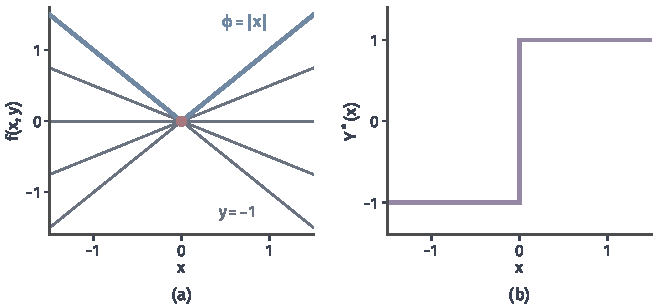
\includegraphics[width=112mm]{figures/05-optimization/07-multiple-criteria-and-nested-optimization/matplotlib/minimax-response-switch/figure.pdf}
 \caption{$f(x,y)=xy$，$Y=[-1,1]$。(a)灰线是$y=0,\pm\frac12,\pm1$时的直线，蓝线是上边缘$\phi(x)=\lvert x\rvert$，红点是外层最优解。(b)紫线是最优响应集合$Y^\star(x)$的图像，在$x=0$处是一整条竖直线段。}
 \label{fig:minimax-response-switch}
\end{BookInlineFigure}

图~\ref{fig:minimax-response-switch}(b)画出了$Y^\star(x)$。在$x\neq0$处它是单点，在$x=0$处是整个区间，这说明最优响应应当看作集合值映射。$(x-y)^2$的情形更极端：$Y^\star(0)=\{-1,1\}$是两个分开的点，集合甚至不连通。

下面的定理给出响应集合紧时能够保证的全部好性质。它说明响应集合可以跳，但图像是闭的，$\phi$本身仍然连续。

\begin{theorem}[紧响应集上的最坏值函数]
\label{thm:minimax-compact}
设$\bm{Y}$非空且紧，$f$在$\bm{X}\times\bm{Y}$上连续。则
\begin{enumerate}
 \item 对每个$\bm{x}\in\bm{X}$，上确界达到，$\bm{Y}^\star(\bm{x})$非空且紧；
 \item $\phi$在$\bm{X}$上有限且连续；
 \item 若$\bm{x}_k\to\bm{x}$，$\bm{y}_k\in\bm{Y}^\star(\bm{x}_k)$，$\bm{y}_k\to\bar{\bm{y}}$，则$\bar{\bm{y}}\in\bm{Y}^\star(\bm{x})$。
\end{enumerate}
\end{theorem}

\begin{proof}
第一条。$f(\bm{x},\cdot)$是紧集上的连续函数，最大值存在。$\bm{Y}^\star(\bm{x})$是连续函数$f(\bm{x},\cdot)$的水平集，是紧集$\bm{Y}$的闭子集，所以紧。

第二条。设$\bm{x}_k\to\bm{x}$。集合$\bm{K}=\{\bm{x}_k\}\cup\{\bm{x}\}$是紧的，$f$在紧集$\bm{K}\times\bm{Y}$上一致连续。记
\[
 \delta_k=\max_{\bm{y}\in\bm{Y}}\lvert f(\bm{x}_k,\bm{y})-f(\bm{x},\bm{y})\rvert\to0.
\]
对任意$\bm{y}$，有
\[
 f(\bm{x}_k,\bm{y})\leq f(\bm{x},\bm{y})+\delta_k\leq\phi(\bm{x})+\delta_k.
\]
对$\bm{y}$取最大，得到$\phi(\bm{x}_k)\leq\phi(\bm{x})+\delta_k$。交换$\bm{x}_k$与$\bm{x}$的角色，得到$\phi(\bm{x})\leq\phi(\bm{x}_k)+\delta_k$。所以$\phi(\bm{x}_k)\to\phi(\bm{x})$。

第三条。由$\bm{y}_k$的最优性，$f(\bm{x}_k,\bm{y}_k)=\phi(\bm{x}_k)$。令$k\to\infty$，用$f$和$\phi$的连续性，得到$f(\bm{x},\bar{\bm{y}})=\phi(\bm{x})$。
\end{proof}

第三条对应图~\ref{fig:minimax-response-switch}(b)的形状：从左右两侧趋于$x=0$时响应趋于$\pm1$，这两个极限都落在$Y^\star(0)$里。反过来不成立，$Y^\star(0)$中的$y=\frac12$不是任何邻近点响应的极限，所以这个映射不是连续的。

\subsection{值函数导数}
\label{sec:minimax-danskin}

要用梯度类方法更新$\bm{x}$，需要$\phi$的导数，而$\phi$本身没有显式表达式。能不能不微分内层的解？

看图~\ref{fig:minimax-danskin}(a)。在$x=0.5$处，起作用的是$y=-1$这条抛物线，上边缘在这里与它相切。切线的斜率就是这条抛物线在$x=0.5$处关于$x$的导数。$y$本身随$x$怎样变，在一阶上不起作用，因为$y$已经处在最优位置，朝任何可行方向挪动，代价都不会一阶增加。

第~\ref{chap:parametric-sensitivity}章的Danskin型结果给出了精确的说法。那里研究固定集合$\bm{C}$上的最优值函数$V(\bm{\theta})$，把它用到$-f$上，记号换成本章的，就得到下面的结论，证明见该章。

\begin{theorem}[最坏值函数的方向导数]
\label{thm:minimax-danskin}
设$\bm{X}\subseteq\mathbb{R}^{n}$开，$\bm{Y}$非空且紧，$f$与$\nabla_{\bm{x}}f$在$\bm{X}\times\bm{Y}$上连续。则对每个$\bm{x}\in\bm{X}$和方向$\bm{d}$，
\begin{equation}
 \phi'(\bm{x};\bm{d})=\max_{\bm{y}\in\bm{Y}^\star(\bm{x})}\bigl\langle\nabla_{\bm{x}}f(\bm{x},\bm{y}),\bm{d}\bigr\rangle.
 \label{eq:minimax-danskin}
\end{equation}
若$\bm{Y}^\star(\bm{x})=\{\bm{y}^\star(\bm{x})\}$是单点，则$\phi$在$\bm{x}$处可微，且
\begin{equation}
 \nabla\phi(\bm{x})=\nabla_{\bm{x}}f(\bm{x},\bm{y}^\star(\bm{x})).
 \label{eq:minimax-danskin-gradient}
\end{equation}
\end{theorem}

式~\eqref{eq:minimax-danskin}取最大值，是因为沿方向$\bm{d}$走一小步之后，起作用的是在这个方向上增长最快的那条响应。在开头的例子里，$\nabla_xf=2(x-y)$。$x=0.5$时响应唯一，$y^\star=-1$，式~\eqref{eq:minimax-danskin-gradient}给出
\[
 \phi'(0.5)=2(0.5+1)=3.
\]
它与直接求导$\phi'(x)=2(x+1)$的结果一致。

在$x=0$处，$Y^\star(0)=\{-1,1\}$，两个响应的偏导数是$2$和$-2$。式~\eqref{eq:minimax-danskin}给出
\[
 \phi'(0;d)=\max\{2d,-2d\}=2\lvert d\rvert.
\]
直接展开，得到
\[
 \phi(d)-\phi(0)=(\lvert d\rvert+1)^2-1=2\lvert d\rvert+d^2,
\]
一阶部分相同。

\begin{BookInlineFigure}
 \centering
 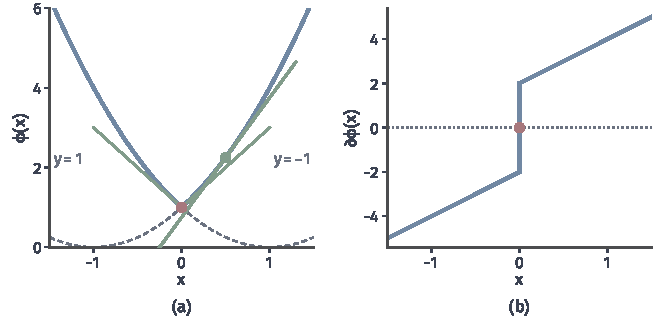
\includegraphics[width=112mm]{figures/05-optimization/07-multiple-criteria-and-nested-optimization/matplotlib/minimax-danskin/figure.pdf}
 \caption{$\phi(x)=(\lvert x\rvert+1)^2$的导数信息。(a)灰色虚线是$y=\pm1$两条抛物线，蓝线是上边缘。绿点$x=0.5$处只有一条活动响应，绿线是斜率为$3$的切线。红点$x=0$处两条响应同时活动，两段绿线的斜率是$\pm2$。(b)次微分的集值图像，在$x=0$处是竖直线段$[-2,2]$，它穿过点线$0$，说明$x=0$是最优解。}
 \label{fig:minimax-danskin}
\end{BookInlineFigure}

\paragraph{条件的作用}
定理要求响应集固定。这个条件去掉，公式就错了。取$f(x,y)=y$，让响应集随方案移动，$Y(x)=[-1,x]$，$x>-1$。则$\phi(x)=x$，导数是$1$，而$\partial f/\partial x\equiv0$。漏掉的部分来自集合边界的移动，要由乘子计入，这正是第~\ref{chap:parametric-sensitivity}章一般含参约束的内容。本章$\bm{Y}$不依赖$\bm{x}$，这个问题不出现。

紧性也不能省。$\bm{Y}$不紧时响应可能不存在，式~\eqref{eq:minimax-danskin}的右端失去意义，表~\ref{tab:minimax-three-levels}第二行就是这样。

\paragraph{关于$\bm{x}$凸时的次梯度集合}
多响应时只有方向导数还不够方便。若$f$关于$\bm{x}$凸，$\phi$是凸函数，可以用第~\ref{chap:nonsmooth-composite-optimization}章的次微分：$\bm{g}$是$\phi$在$\bm{x}$处的次梯度，指对所有$\bm{x}'$都有
\[
 \phi(\bm{x}')\geq\phi(\bm{x})+\langle\bm{g},\bm{x}'-\bm{x}\rangle.
\]

该章对有限个函数的最大值证明了次微分是活跃梯度的凸包，下面的定理把分支数推广到紧集上的无穷多个。

\begin{theorem}[最坏值函数的次微分]
\label{thm:minimax-subdiff}
设$\bm{X}=\mathbb{R}^{n}$，$\bm{Y}$非空且紧，$f$与$\nabla_{\bm{x}}f$连续，且对每个$\bm{y}\in\bm{Y}$，$f(\cdot,\bm{y})$是凸函数。则
\begin{equation}
 \partial\phi(\bm{x})=\operatorname{conv}\bigl\{\nabla_{\bm{x}}f(\bm{x},\bm{y}):\bm{y}\in\bm{Y}^\star(\bm{x})\bigr\}.
 \label{eq:minimax-subdiff}
\end{equation}
\end{theorem}

\begin{proof}
记右端为$\bm{K}$。$\bm{Y}^\star(\bm{x})$是紧集，它在连续映射$\nabla_{\bm{x}}f(\bm{x},\cdot)$下的像也是紧集，$\mathbb{R}^n$中紧集的凸包仍是紧集，所以$\bm{K}$紧且凸。

先证$\bm{K}\subseteq\partial\phi(\bm{x})$。任取$\bm{y}\in\bm{Y}^\star(\bm{x})$和$\bm{x}'$。由$\phi$的定义和$f(\cdot,\bm{y})$的凸性，
\[
 \phi(\bm{x}')\geq f(\bm{x}',\bm{y})\geq f(\bm{x},\bm{y})+\langle\nabla_{\bm{x}}f(\bm{x},\bm{y}),\bm{x}'-\bm{x}\rangle.
\]
左边第二项的$f(\bm{x},\bm{y})$等于$\phi(\bm{x})$。把这样的不等式按凸组合的权重相加，右端的向量就换成了$\bm{K}$中的任意元素。

再证反向。设$\bm{g}\in\partial\phi(\bm{x})$但$\bm{g}\notin\bm{K}$。$\bm{K}$非空、闭、凸，由第~\ref{chap:duality}章点与闭凸集的严格分离，存在$\bm{d}$，使
\[
 \langle\bm{g},\bm{d}\rangle>\max_{\bm{c}\in\bm{K}}\langle\bm{c},\bm{d}\rangle\geq\max_{\bm{y}\in\bm{Y}^\star(\bm{x})}\langle\nabla_{\bm{x}}f(\bm{x},\bm{y}),\bm{d}\rangle=\phi'(\bm{x};\bm{d}).
\]
最后的等号是式~\eqref{eq:minimax-danskin}。

另一方面，次梯度不等式给出
\[
 \phi(\bm{x}+s\bm{d})-\phi(\bm{x})\geq s\langle\bm{g},\bm{d}\rangle.
\]
除以$s>0$并令$s\downarrow0$，得到
\[
 \phi'(\bm{x};\bm{d})\geq\langle\bm{g},\bm{d}\rangle.
\]
这与上式矛盾。
\end{proof}

对开头的例子，活动偏导数是$\pm2$，所以$\partial\phi(0)=[-2,2]$，见图~\ref{fig:minimax-danskin}(b)。对$f=xy$，活动偏导数是$\lvert y\rvert\leq1$的全体$y$，所以$\partial\phi(0)=[-1,1]$。两者都含$0$，所以$x=0$都是全局最优解。

多响应时要注意一件事：只取其中一个响应，它给出的梯度未必是下降方向。在$(x-y)^2$的$x=0$处，取$y=1$，偏导数是$-2$，沿负偏导数方向是把$x$往正的方向移，而$\phi$沿这个方向是上升的。这和第~\ref{chap:nonsmooth-composite-optimization}章次梯度的负方向未必下降是同一回事。值函数的导数和次梯度只回答“外层目标对$\bm{x}$怎样变化”；$\bm{Y}$或约束也随参数变化时的完整敏感性，由第~\ref{chap:parametric-sensitivity}章处理。

\section{鞍点}
\label{sec:minimax-saddle}

判断一个$\bm{x}$好不好，要算$\phi(\bm{x})$，也就要解一次内层。如果手上同时有一个$\bm{x}$和一个$\bm{y}$，能不能让它们互相作证？本节研究这样一对候选应当满足什么关系，它和两个次序的值有什么联系。

记交换次序后的函数为
\begin{equation}
 \psi(\bm{y})=\inf_{\bm{x}\in\bm{X}}f(\bm{x},\bm{y}),
 \label{eq:minimax-psi}
\end{equation}
它是$\bm{y}$先定时外层能做到的最好代价。两个次序的值分别记作
\begin{equation}
 \bar{v}=\inf_{\bm{x}\in\bm{X}}\phi(\bm{x}),\qquad\underline{v}=\sup_{\bm{y}\in\bm{Y}}\psi(\bm{y}).
 \label{eq:minimax-values}
\end{equation}
式~\eqref{eq:minimax-weak}就是$\underline{v}\leq\bar{v}$。

想象一个山口。沿着山脊方向，山口是最低点；沿着翻山的方向，山口是最高点。站在山口，往山脊两头走都要上坡，往两侧山谷走都要下坡。下面的定义把这个图景用到两组变量上：沿$\bm{x}$的方向山口最低，沿$\bm{y}$的方向山口最高。

\begin{definition}[全局鞍点]
\label{def:minimax-saddle}
若$(\bm{x}^\star,\bm{y}^\star)\in\bm{X}\times\bm{Y}$对所有$\bm{x}\in\bm{X}$，$\bm{y}\in\bm{Y}$满足
\begin{equation}
 f(\bm{x}^\star,\bm{y})\leq f(\bm{x}^\star,\bm{y}^\star)\leq f(\bm{x},\bm{y}^\star),
 \label{eq:minimax-saddle}
\end{equation}
就称它是$f$在$\bm{X}\times\bm{Y}$上的\term{全局鞍点}（global saddle point）。
\end{definition}

式~\eqref{eq:minimax-saddle}的右半边说，固定$\bm{y}^\star$时$\bm{x}^\star$全局最小；左半边说，固定$\bm{x}^\star$时$\bm{y}^\star$全局最大。任何一侧单独改变，都不能改善自己的目标。山口的类比在这里到头了：山的形状只有一种，而鞍点还取决于哪个变量要最小化、哪个要最大化。

这个定义比第~\ref{chap:saddle-points}章的鞍点多了分工。那一章的鞍点指Hessian不定的驻点，只看函数形状，不问变量的角色。

要把几个相近的概念分开，看图~\ref{fig:minimax-saddle-types}中的三个二次函数，以及后面一个四次函数。$x$是外层变量，$y$是内层变量。

\begin{BookInlineFigure}
 \centering
 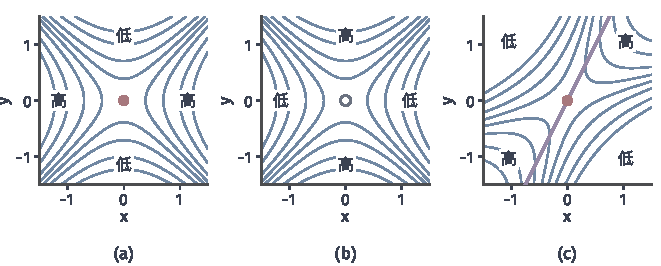
\includegraphics[width=112mm]{figures/05-optimization/07-multiple-criteria-and-nested-optimization/matplotlib/minimax-saddle-types/figure.pdf}
 \caption{原点都是两侧一阶驻定点，蓝线是等高线，“高”“低”标出函数值的高低区域。(a)$x^2-y^2$：沿$x$最小、沿$y$最大，红点是全局鞍点。(b)$y^2-x^2$：形状相同而角色相反，空心点既不是鞍点，也不解决顺序问题。(c)$-\frac12x^2+2xy-\frac12y^2$：紫线是最优响应$y=2x$，红点解决顺序问题，却不是鞍点。}
 \label{fig:minimax-saddle-types}
\end{BookInlineFigure}

(a)的$f=x^2-y^2$在全平面满足式~\eqref{eq:minimax-saddle}，原点是全局鞍点。(b)的$f=y^2-x^2$在原点的两个偏导数也都为零，但固定$y=0$时$-x^2$在$x=0$处最大，外层变量离开原点反而更好。

(c)最值得留意。取$f=-\frac12x^2+2xy-\frac12y^2$，$X=Y=\mathbb{R}$。这个函数在本章后面反复使用。内层关于$y$严格凹，令$\partial_yf=2x-y=0$，得$y^\star(x)=2x$。代回得到
\begin{equation}
 \phi(x)=-\frac12x^2+4x^2-2x^2=\frac32x^2.
 \label{eq:minimax-running-phi}
\end{equation}

$\phi$的最小点是$x=0$，顺序问题的解是原点，值是$0$。可是固定$y=0$时$f(x,0)=-\frac12x^2$在$x=0$处最大，式~\eqref{eq:minimax-saddle}的右半边不成立。对任意$y$，$\psi(y)=\inf_xf=-\infty$，所以$\underline{v}=-\infty<0=\bar{v}$。外层在这里不是对$\bm{x}$最小化固定的$f$，它考虑的是$y$会跟着$x$一起变，这个跟随效应把$-\frac12x^2$的向下弯曲翻了过来。

局部的版本是把式~\eqref{eq:minimax-saddle}中的“所有”改成“$(\bm{x}^\star,\bm{y}^\star)$某个邻域内的所有”，称为\term{局部鞍点}（local saddle point）。例如在$X=[-3,3]$，$Y=[-1,1]$上取
\begin{equation}
 f(x,y)=x^2-\frac14x^4-y^2.
 \label{eq:minimax-local-saddle}
\end{equation}
在原点附近$x^2-\frac14x^4\geq0$，所以原点是局部鞍点。但$f(3,0)=9-\frac{81}{4}=-11.25<0$，外层变量跑远了反而更好，所以原点不是全局鞍点。

\begin{BookInlineTable}
 \centering
 \begin{tabular}{@{}lll@{}}
  \toprule
  概念 & 要求 & 例子\\
  \midrule
  两侧一阶驻定 & 无约束时两个偏梯度为零 & 图~\ref{fig:minimax-saddle-types}三个原点\\
  局部鞍点 & 式~\eqref{eq:minimax-saddle}在邻域内成立 & 式~\eqref{eq:minimax-local-saddle}的原点\\
  全局鞍点 & 式~\eqref{eq:minimax-saddle}在全域成立 & $x^2-y^2$的原点\\
  顺序问题的解 & $\bm{x}$最小化$\phi$ & 图~\ref{fig:minimax-saddle-types}(c)的原点\\
  \bottomrule
 \end{tabular}
 \caption{四个相近概念的比较。两侧一阶驻定最弱，它不自动解决顺序问题；顺序问题的解也不一定是鞍点。}
 \label{tab:minimax-saddle-compare}
\end{BookInlineTable}

全局鞍点与两个次序的关系，由下面的定理给出。

\begin{theorem}[鞍点与最值相等]
\label{thm:minimax-saddle-values}
设$\bm{x}^\star\in\bm{X}$，$\bm{y}^\star\in\bm{Y}$。$(\bm{x}^\star,\bm{y}^\star)$是全局鞍点，当且仅当同时满足
\begin{equation}
 \phi(\bm{x}^\star)=\bar{v},\qquad\psi(\bm{y}^\star)=\underline{v},\qquad\bar{v}=\underline{v}\in\mathbb{R}.
 \label{eq:minimax-saddle-values}
\end{equation}
此时共同的值等于$f(\bm{x}^\star,\bm{y}^\star)$。
\end{theorem}

\begin{proof}
必要性。对式~\eqref{eq:minimax-saddle}的左半边取$\bm{y}$的上确界，右半边取$\bm{x}$的下确界，得到
\[
 \phi(\bm{x}^\star)\leq f(\bm{x}^\star,\bm{y}^\star)\leq\psi(\bm{y}^\star).
\]
结合定义，又有
\[
 \underline{v}\leq\bar{v}\leq\phi(\bm{x}^\star),\qquad\psi(\bm{y}^\star)\leq\underline{v}.
\]
把这些不等式连起来，就成为一个闭环，其中所有的量都相等。

充分性。由式~\eqref{eq:minimax-saddle-values}，$\phi(\bm{x}^\star)=\psi(\bm{y}^\star)$是有限数。定义给出
\[
 \psi(\bm{y}^\star)\leq f(\bm{x}^\star,\bm{y}^\star)\leq\phi(\bm{x}^\star),
\]
所以三者相等。于是对任意$\bm{x},\bm{y}$，
\[
 f(\bm{x}^\star,\bm{y})\leq\phi(\bm{x}^\star)=\psi(\bm{y}^\star)\leq f(\bm{x},\bm{y}^\star),
\]
中间的值等于$f(\bm{x}^\star,\bm{y}^\star)$，这就是式~\eqref{eq:minimax-saddle}。
\end{proof}

定理说明鞍点集合是一个乘积集合。若$(\bm{x}_1,\bm{y}_1)$和$(\bm{x}_2,\bm{y}_2)$都是鞍点，式~\eqref{eq:minimax-saddle-values}的三条对$(\bm{x}_1,\bm{y}_2)$同样成立，所以它也是鞍点，不需要把两侧配对寻找。这与第~\ref{chap:duality}章的Lagrange鞍点定理一致，那里的$\mathcal{L}$就是这里的$f$。

\subsection{最值交换}
\label{sec:minimax-exchange}

什么条件能让$\underline{v}=\bar{v}$？先回到图~\ref{fig:minimax-cost-table}的代价表，看一个修复办法。两个次序之所以不同，是因为每一方只能选一个端点。设想方案可以按比例组合：把份额$p$投给方案$\mathrm{a}$，$1-p$投给方案$\mathrm{b}$；扰动也按比例$q$和$1-q$作用，代价按份额加权。

记$p,q\in[0,1]$，代价为
\[
 f(p,q)=3pq+p(1-q)+2(1-p)(1-q).
\]
展开并配方，得到
\begin{equation}
 f(p,q)=4pq-p-2q+2=4\Bigl(p-\frac12\Bigr)\Bigl(q-\frac14\Bigr)+\frac32.
 \label{eq:minimax-relaxed}
\end{equation}

$f$关于$q$是线性的，最大值在端点取到，所以
\[
 \phi(p)=\max\{f(p,0),f(p,1)\}=\max\{2-p,3p\}.
\]
同理，$f$关于$p$线性，最小值在端点取到，所以
\[
 \psi(q)=\min\{f(0,q),f(1,q)\}=\min\{2-2q,1+2q\}.
\]

$\phi$在$2-p=3p$即$p=\frac12$处最小，$\psi$在$2-2q=1+2q$即$q=\frac14$处最大，并且
\[
 \phi\Bigl(\frac12\Bigr)=\psi\Bigl(\frac14\Bigr)=\frac32.
\]
由定理~\ref{thm:minimax-saddle-values}，$(\frac12,\frac14)$是鞍点，见图~\ref{fig:minimax-relaxed-table}。两个次序现在给出同一个值$\frac32$，它落在原来的$1$和$2$之间。允许按比例组合，也就是把问题做成关于各自变量线性的，先后的差别消失了。

\begin{BookInlineFigure}
 \centering
 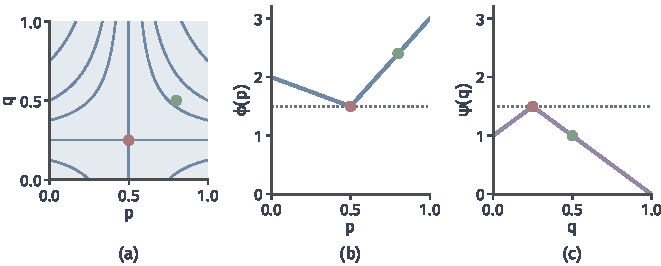
\includegraphics[width=112mm]{figures/05-optimization/07-multiple-criteria-and-nested-optimization/matplotlib/minimax-relaxed-table/figure.pdf}
 \caption{代价表的比例松弛$f(p,q)=4(p-\frac12)(q-\frac14)+\frac32$。(a)浅蓝是可行域，蓝线是等高线，穿过红点的十字是值为$\frac32$的等高线，红点是鞍点，绿点是候选$(0.8,0.5)$。(b)外层目标$\phi(p)$，红点是最小点。(c)$\psi(q)$，红点是最大点。点线是共同的值$\frac32$，绿点是候选在两条曲线上的值。}
 \label{fig:minimax-relaxed-table}
\end{BookInlineFigure}

这个例子的结构可以一般化：两个集合都是紧凸集，$f$关于$\bm{x}$凸、关于$\bm{y}$凹。凸凹性是说，混合之后不会比原来更有利于对面。

\begin{theorem}[紧集上的极小极大定理]
\label{thm:minimax-theorem}
设$\bm{X},\bm{Y}$非空、紧、凸，$f$在$\bm{X}\times\bm{Y}$上连续；对每个$\bm{y}\in\bm{Y}$，$f(\cdot,\bm{y})$是凸函数；对每个$\bm{x}\in\bm{X}$，$f(\bm{x},\cdot)$是凹函数。则
\begin{equation}
 \min_{\bm{x}\in\bm{X}}\max_{\bm{y}\in\bm{Y}}f(\bm{x},\bm{y})=\max_{\bm{y}\in\bm{Y}}\min_{\bm{x}\in\bm{X}}f(\bm{x},\bm{y}),
 \label{eq:minimax-theorem}
\end{equation}
两侧的最值都达到，并且存在全局鞍点。
\end{theorem}

\begin{proof}
由式~\eqref{eq:minimax-weak}，只需排除$\underline{v}<\bar{v}$。用反证法，设$\underline{v}<\bar{v}$，取实数$c$满足$\underline{v}<c<\bar{v}$。

第一步，把无穷多个$\bm{y}$化成有限个。对每个$\bm{x}\in\bm{X}$，有$\phi(\bm{x})\geq\bar{v}>c$，所以存在$\bm{y}$使$f(\bm{x},\bm{y})>c$。于是开集族
\[
 \bm{U}_{\bm{y}}=\{\bm{x}\in\bm{X}:f(\bm{x},\bm{y})>c\},\qquad\bm{y}\in\bm{Y}
\]
覆盖了$\bm{X}$。$\bm{X}$是紧集，存在有限个$\bm{y}_1,\ldots,\bm{y}_k$，使每个$\bm{x}\in\bm{X}$都至少满足一条$f(\bm{x},\bm{y}_i)>c$。

第二步，用凸性分离出权重。令
\[
 \bm{S}=\bigl\{\bm{w}\in\mathbb{R}^k:\text{存在}\ \bm{x}\in\bm{X},\ \text{使}\ w_i\geq f(\bm{x},\bm{y}_i)\ \text{对所有}\ i\ \text{成立}\bigr\}.
\]
$\bm{X}$是凸集，每个$f(\cdot,\bm{y}_i)$是凸函数，所以$\bm{S}$是凸集。点$\bm{c}=(c,\ldots,c)$不在$\bm{S}$中，否则某个$\bm{x}$使所有$f(\bm{x},\bm{y}_i)\leq c$，与第一步矛盾。

第~\ref{chap:duality}章的点与凸集分离引理不要求$\bm{S}$闭，由它得到$\bm{a}\neq\bm{0}$，使
\[
 \langle\bm{a},\bm{w}\rangle\geq\langle\bm{a},\bm{c}\rangle\qquad\text{对所有}\ \bm{w}\in\bm{S}.
\]
$\bm{S}$中的点把任一分量增大后仍在$\bm{S}$中。若某个$a_i<0$，让$w_i\to+\infty$，左端趋于$-\infty$，矛盾。所以$\bm{a}\geq\bm{0}$，可以归一化为$\sum_ia_i=1$，此时$\langle\bm{a},\bm{c}\rangle=c$。

对任意$\bm{x}\in\bm{X}$，取$w_i=f(\bm{x},\bm{y}_i)$，得到
\[
 \sum_{i=1}^ka_if(\bm{x},\bm{y}_i)\geq c.
\]

第三步，用凹性把有限个$\bm{y}_i$合成一个。令$\bar{\bm{y}}=\sum_ia_i\bm{y}_i$。$\bm{Y}$是凸集，所以$\bar{\bm{y}}\in\bm{Y}$。$f(\bm{x},\cdot)$是凹函数，所以对所有$\bm{x}\in\bm{X}$，
\[
 f(\bm{x},\bar{\bm{y}})\geq\sum_{i=1}^ka_if(\bm{x},\bm{y}_i)\geq c.
\]
于是$\psi(\bar{\bm{y}})\geq c>\underline{v}$，与$\underline{v}$是$\psi$的上确界矛盾。所以$\underline{v}=\bar{v}$。

最后看达到。由定理~\ref{thm:minimax-compact}，$\phi$在紧集$\bm{X}$上连续，最小值达到；对$-f$用同一定理，$\psi$在紧集$\bm{Y}$上连续，最大值达到。取最优点$\bm{x}^\star,\bm{y}^\star$，由定理~\ref{thm:minimax-saddle-values}，它们组成全局鞍点。
\end{proof}

证明里每个条件各有职责。$\bm{X}$紧把无穷多个响应化为有限个；关于$\bm{x}$的凸性使$\bm{S}$凸，因而能分离出权重；关于$\bm{y}$的凹性与$\bm{Y}$的凸性把“按权重混合的$\bm{y}_i$”合成$\bm{Y}$中的一个点。开头的$(x-y)^2$缺的是最后一条：$f$关于$y$是凸的，端点$y=\pm1$按等权混合的代价是$x^2+1$，而单点$y=0$的代价只有$x^2$，混合无法用一个$y$代替。

\paragraph{放宽紧性时要分别核对}
更一般的Sion定理只要求其中一个集合紧，把凸凹性放宽为拟凸拟凹，连续性放宽为半连续，结论仍是两个次序的值相等\scite{sion1958}。它的证明需要一套关于水平集连通性的论证，篇幅较长。这里用两个例子说明放宽之后什么会失去。

两个集合都不紧时，值可能不相等。在$X=Y=[0,\infty)$上取
\[
 f(x,y)=\frac{y-x}{1+x+y}.
\]
由于$f=-1+\frac{1+2y}{1+x+y}$，它关于$x$凸；由于$f=1-\frac{1+2x}{1+x+y}$，它关于$y$凹。令$y\to\infty$得$\phi(x)=1$，令$x\to\infty$得$\psi(y)=-1$，所以$\bar{v}=1$，$\underline{v}=-1$。这里凸凹性和连续性都有，只是少了紧性，见图~\ref{fig:minimax-exchange-fail}(a)。

值相等也不等于鞍点存在。在$X=[0,\infty)$，$Y=[0,1]$上取$f(x,y)=ye^{-x}$，满足Sion定理的条件。内层取$y=1$，得$\phi(x)=e^{-x}$，它的下确界是$0$，但没有$x$取到；外层令$x\to\infty$，得$\psi(y)=0$。所以$\bar{v}=\underline{v}=0$，而没有$x$使$\phi(x)=0$，由定理~\ref{thm:minimax-saddle-values}，鞍点不存在，见图~\ref{fig:minimax-exchange-fail}(b)。

\begin{BookInlineFigure}
 \centering
 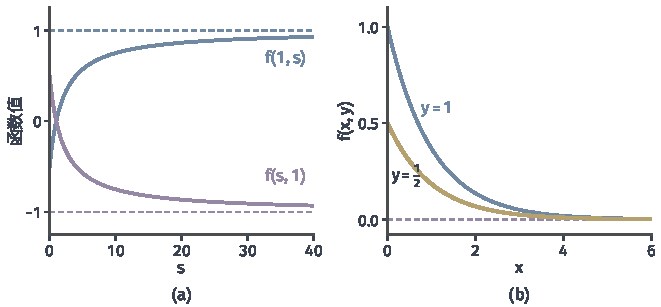
\includegraphics[width=112mm]{figures/05-optimization/07-multiple-criteria-and-nested-optimization/matplotlib/minimax-exchange-fail/figure.pdf}
 \caption{放宽紧性的两种后果。(a)$f=(y-x)/(1+x+y)$在$[0,\infty)^2$上：蓝线$f(1,s)$沿$y=s$趋于蓝色虚线$1$，紫线$f(s,1)$沿$x=s$趋于紫色虚线$-1$，两个次序的值不同。(b)$f=ye^{-x}$：蓝线和黄线分别是$y=1,\frac12$时的截线，都趋于紫色虚线$0$而取不到，值相等但没有鞍点。}
 \label{fig:minimax-exchange-fail}
\end{BookInlineFigure}

最值相等是一个关于数的结论。要从中取出一对点，还必须分别核对$\phi$的最小值和$\psi$的最大值是否达到。

\subsection{鞍点间隙}
\label{sec:minimax-gap}

有了$\phi$和$\psi$，就能给任何一对可行候选打分。这是第~\ref{chap:duality}章“可行点给上界、乘子给下界”的直接推广。

\begin{definition}[鞍点间隙]
\label{def:minimax-gap}
对$(\bm{x},\bm{y})\in\bm{X}\times\bm{Y}$，定义
\begin{equation}
 G(\bm{x},\bm{y})=\sup_{\bm{v}\in\bm{Y}}f(\bm{x},\bm{v})-\inf_{\bm{u}\in\bm{X}}f(\bm{u},\bm{y})=\phi(\bm{x})-\psi(\bm{y}),
 \label{eq:minimax-gap}
\end{equation}
称为\term{鞍点间隙}（saddle gap），其中$\phi(\bm{x})=+\infty$或$\psi(\bm{y})=-\infty$时$G=+\infty$。
\end{definition}

间隙度量的是：固定对方，各自还能改善多少，两边加起来。

\begin{theorem}[间隙是全局证书]
\label{thm:minimax-gap}
对任意$(\bm{x},\bm{y})\in\bm{X}\times\bm{Y}$，只要$G(\bm{x},\bm{y})$有定义，就有$G(\bm{x},\bm{y})\geq\bar{v}-\underline{v}\geq0$，并且
\begin{equation}
 \phi(\bm{x})-\bar{v}\leq G(\bm{x},\bm{y}),\qquad\underline{v}-\psi(\bm{y})\leq G(\bm{x},\bm{y}).
 \label{eq:minimax-gap-bound}
\end{equation}
当$G(\bm{x},\bm{y})$有限时，$G(\bm{x},\bm{y})=0$当且仅当$(\bm{x},\bm{y})$是全局鞍点。
\end{theorem}

\begin{proof}
由定义，$\phi(\bm{x})\geq\bar{v}$，$\psi(\bm{y})\leq\underline{v}$，相减得$G\geq\bar{v}-\underline{v}$，它由式~\eqref{eq:minimax-weak}非负。

式~\eqref{eq:minimax-gap-bound}的第一式等价于$\psi(\bm{y})\leq\bar{v}$，它由$\psi(\bm{y})\leq\underline{v}\leq\bar{v}$得到。第二式等价于$\underline{v}\leq\phi(\bm{x})$，它由$\underline{v}\leq\bar{v}\leq\phi(\bm{x})$得到。

若$G=0$，由上面的不等式，$\phi(\bm{x})=\bar{v}$，$\psi(\bm{y})=\underline{v}$，且$\bar{v}=\underline{v}$，由定理~\ref{thm:minimax-saddle-values}它是全局鞍点。反过来，全局鞍点满足式~\eqref{eq:minimax-saddle-values}，相减为零。
\end{proof}

式~\eqref{eq:minimax-gap-bound}是最有用的部分。它不需要知道$\bar{v}$，就能说出$\bm{x}$的最坏值离最优最多差多少。回到比例松弛，取图~\ref{fig:minimax-relaxed-table}的绿点$(p,q)=(0.8,0.5)$，算得
\[
 \phi(0.8)=\max\{1.2,2.4\}=2.4,\qquad\psi(0.5)=\min\{1,2\}=1.
\]
所以
\[
 G(0.8,0.5)=1.4.
\]
真实的次优量是$\phi(0.8)-\frac32=0.9$，确实不超过$1.4$。

对$f=xy$，$X=Y=[-1,1]$，有
\begin{equation}
 \phi(x)=\lvert x\rvert,\qquad\psi(y)=-\lvert y\rvert,\qquad G(x,y)=\lvert x\rvert+\lvert y\rvert.
 \label{eq:minimax-box-gap}
\end{equation}
这个例子的答案可以直接读出来，后面却会看到，最直接的算法在它上面就会失败。

\paragraph{非紧域上的间隙}
把上面的集合换成$X=Y=\mathbb{R}$，同一个$f=xy$的$\phi(x)$在$x\neq0$时是$+\infty$，于是$G$除了原点处处是$+\infty$。此时$G$虽然没有错，却完全不能区分候选的好坏。

常见的处理是只在一个有界区域$\bm{B}=\bm{B}_{\bm{X}}\times\bm{B}_{\bm{Y}}$上取极值，其中$\bm{B}_{\bm{X}}\subseteq\bm{X}$，$\bm{B}_{\bm{Y}}\subseteq\bm{Y}$，候选在$\bm{B}$内，得到
\begin{equation}
 G_{\bm{B}}(\bm{x},\bm{y})=\sup_{\bm{v}\in\bm{B}_{\bm{Y}}}f(\bm{x},\bm{v})-\inf_{\bm{u}\in\bm{B}_{\bm{X}}}f(\bm{u},\bm{y}).
 \label{eq:minimax-restricted-gap}
\end{equation}

称为\term{限定间隙}（restricted gap）。上确界和下确界的范围变小，所以$G_{\bm{B}}\leq G$。它是真实间隙的下估计，小的$G_{\bm{B}}$不能说明$G$小。

式~\eqref{eq:minimax-local-saddle}正好说明这一点。取$\bm{B}=[-1,1]\times[-1,1]$，候选为原点。在$\bm{B}$内$x^2-\frac14x^4\geq0$，$-y^2\leq0$，所以$G_{\bm{B}}(0,0)=0$。但在整个$X=[-3,3]$上，
\[
 \psi(0)=\min_{\lvert u\rvert\leq3}\Bigl(u^2-\frac14u^4\Bigr)=-11.25,\qquad\phi(0)=0.
\]
所以真实间隙是$11.25$，见图~\ref{fig:minimax-restricted-gap}。局部检验框看不到框外的低谷，零的限定间隙不能当作全局证书。

\begin{BookInlineFigure}
 \centering
 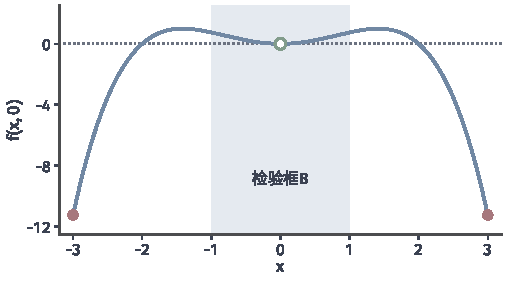
\includegraphics[width=86mm]{figures/05-optimization/07-multiple-criteria-and-nested-optimization/matplotlib/minimax-restricted-gap/figure.pdf}
 \caption{$f(x,y)=x^2-\frac14x^4-y^2$在$y=0$上的截线，$X=[-3,3]$。浅蓝区域是检验框，框内原点（绿色空心点）的值最小，限定间隙为零。红点是框外的真正最小点，值为$-11.25$，真实间隙是$11.25$。}
 \label{fig:minimax-restricted-gap}
\end{BookInlineFigure}

凸凹问题里限定间隙的意义强一些。若$\bm{B}$内含有一个全局鞍点$(\bm{x}^\star,\bm{y}^\star)$，则
\[
 G_{\bm{B}}(\bm{x},\bm{y})\geq f(\bm{x},\bm{y}^\star)-f(\bm{x}^\star,\bm{y})\geq0,
\]
所以它至少是一个非负的度量，只要$\bm{B}$足够大，把解包含在内。这条依赖“$\bm{B}$内含解”这个事实，而这个事实本身需要另外的证据。

\section{内层响应法}
\label{sec:minimax-inner-response}

最直接的求解办法是照着决策顺序来：固定当前的$\bm{x}$，先求最坏响应，再用值函数的信息更新$\bm{x}$。外层用什么算法，前面各章已经讲过，本节只回答两个新问题：内层要解到什么程度，内层的误差怎样传到外层。

图~\ref{fig:minimax-response-flow}是整个方法的结构。

\begin{BookInlineFigure}
 \centering
 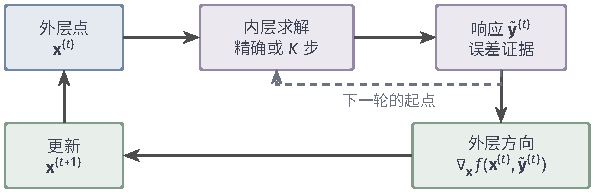
\includegraphics[width=100.7mm]{figures/05-optimization/07-multiple-criteria-and-nested-optimization/tikz/minimax-response-flow/figure.pdf}
 \caption{内层响应法的一轮。紫框是内层计算，绿框是外层计算。内层的输出除了响应，还应带有它的误差证据。虚线表示本轮响应作为下一轮内层的起点。}
 \label{fig:minimax-response-flow}
\end{BookInlineFigure}

\subsection{精确响应}
\label{sec:minimax-exact-response}

\paragraph{主要思想}
设内层最优响应唯一且$\phi$可微。定理~\ref{thm:minimax-danskin}说，算梯度时可以把响应当作常数，所以外层的梯度步就是
\begin{equation}
 \bm{x}^{(t+1)}=P_{\bm{X}}\Bigl(\bm{x}^{(t)}-\alpha\nabla_{\bm{x}}f\bigl(\bm{x}^{(t)},\bm{y}^\star(\bm{x}^{(t)})\bigr)\Bigr),
 \label{eq:minimax-exact-step}
\end{equation}
其中$\bm{X}$是闭凸集，$P_{\bm{X}}$是第~\ref{chap:feasible-iterations}章的欧氏投影，$\bm{X}=\mathbb{R}^n$时投影是恒等映射。这就是对$\phi$做投影梯度法，收敛性由$\phi$的光滑常数和凸性决定，不需要新的理论。

\paragraph{计算过程}
用式~\eqref{eq:minimax-running-phi}的函数演示，$f=-\frac12x^2+2xy-\frac12y^2$，$X=Y=\mathbb{R}$。

\needspace{6\baselineskip}
\paragraph{变量}
\begin{itemize}
 \item $x^{(t)}$：外层变量；
 \item $y^{(t)}$：内层在$x^{(t)}$处的精确响应；
 \item $g^{(t)}$：外层偏导数；
 \item $\alpha>0$：外层步长。
\end{itemize}

\paragraph{初始化}
取$x^{(0)}$。例中$x^{(0)}=1$，步长$\alpha=\frac16$，当$\lvert g^{(t)}\rvert\leq0.4$时停止。

\needspace{6\baselineskip}
\paragraph{每轮更新}
\begin{enumerate}
 \item 解内层，得$y^{(t)}=y^\star(x^{(t)})$。例中$y^\star(x)=2x$，第一轮
 \[
  y^{(0)}=2.
 \]
 \item 计算外层偏导数$g^{(t)}=\partial_xf(x^{(t)},y^{(t)})$。例中$\partial_xf=-x+2y$，第一轮
 \[
  g^{(0)}=-1+4=3.
 \]
 \item 由式~\eqref{eq:minimax-exact-step}更新。例中第一轮
 \[
  x^{(1)}=1-\frac16\cdot3=\frac12.
 \]
\end{enumerate}

第二轮$y^{(1)}=1$，$g^{(1)}=\frac32$，$x^{(2)}=\frac14$。第三轮$y^{(2)}=\frac12$，$g^{(2)}=\frac34$，$x^{(3)}=\frac18$。第四轮$y^{(3)}=\frac14$，$g^{(3)}=\frac38\leq0.4$，停止。

最终得到$x^{(3)}=\frac18$，最坏值$\phi(\frac18)=\frac{3}{128}$。例中$g^{(t)}=\phi'(x^{(t)})=3x^{(t)}$，与式~\eqref{eq:minimax-running-phi}的导数相同，这正是定理~\ref{thm:minimax-danskin}的内容。

\paragraph{响应切换时改用非光滑方法}
$\phi$有折角时，式~\eqref{eq:minimax-exact-step}里的偏梯度只是一个次梯度，而次梯度不随接近解而变小。设$f=(x-y)^2$，$Y=[-1,1]$，$x^{(0)}=0.8$，固定步长$\alpha=0.2$。

$x>0$时最坏响应是$y=-1$，偏导数是$2(x+1)$；$x<0$时最坏响应是$y=1$，偏导数是$2(x-1)$。前三步是
\[
 \begin{aligned}
 x^{(1)}&=0.8-0.2\cdot3.6=0.08,\\
 x^{(2)}&=0.08-0.2\cdot2.16=-0.352,\\
 x^{(3)}&=-0.352+0.2\cdot2.704=0.1888.
 \end{aligned}
\]

迭代很快进入一个周期为$2$的循环。在循环上，$x>0$时映射是$x\mapsto0.6x-0.4$，$x<0$时映射是$x\mapsto0.6x+0.4$，解$a\mapsto-a\mapsto a$得到$a=\frac14$。迭代在$\pm\frac14$之间来回跳，目标差停在$(\frac54)^2-1=0.5625$，见图~\ref{fig:minimax-subgradient-worst}中的黄线。

\begin{BookInlineFigure}
 \centering
 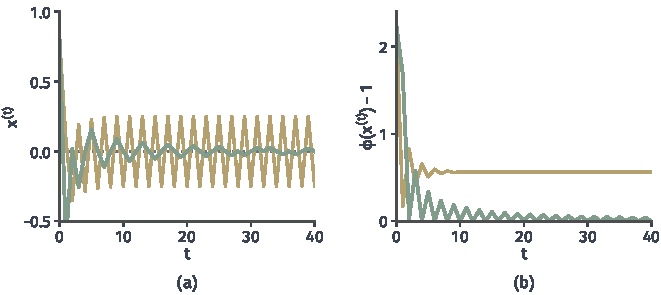
\includegraphics[width=112mm]{figures/05-optimization/07-multiple-criteria-and-nested-optimization/matplotlib/minimax-subgradient-worst/figure.pdf}
 \caption{精确响应加次梯度步，$\phi(x)=(\lvert x\rvert+1)^2$，起点$0.8$。黄线是固定步长$0.2$，绿线是递减步长$0.4/(t+1)$。(a)迭代点：黄线进入$\pm\frac14$的循环，绿线逐渐收敛到最优解$0$。(b)目标差：黄线停在$0.5625$，绿线继续下降。}
 \label{fig:minimax-subgradient-worst}
\end{BookInlineFigure}

这是第~\ref{chap:nonsmooth-composite-optimization}章次梯度法的典型行为，$\phi$是凸函数时那里的结论可以直接使用：有界次梯度下，步长取固定值$R/(G_{\mathrm{b}}\sqrt{T})$时平均点的目标差不超过$RG_{\mathrm{b}}/\sqrt{T}$，其中$R$是起点到解的距离上界，$G_{\mathrm{b}}$是次梯度范数上界。要让误差继续减小，步长必须递减。

\paragraph{局部极大不能代替全局最坏响应}
定理~\ref{thm:minimax-danskin}要的是全局最优响应。内层不凹时，内层算法通常只能找到局部极大点。看下面的函数，$Y=[-2,2]$：
\begin{equation}
 f(x,y)=\frac12x^2+xy+y^2-\frac14y^4.
 \label{eq:minimax-nonconcave}
\end{equation}

固定$x=1$，令$\partial_yf=1+2y-y^3=0$。因式分解得到
\[
 (y+1)(y^2-y-1)=0,
\]
三个根是$y=-1$，$y=\frac{1+\sqrt5}{2}\approx1.618$，$y=\frac{1-\sqrt5}{2}\approx-0.618$。计算得到
\[
 f(1,-1)=0.25,\qquad f(1,1.618)\approx3.023,\qquad f(1,-0.618)\approx0.227.
\]
$y=-1$是局部极大，$y=1.618$是全局极大，$y=-0.618$是局部极小，见图~\ref{fig:minimax-local-response}(a)。

\begin{BookInlineFigure}
 \centering
 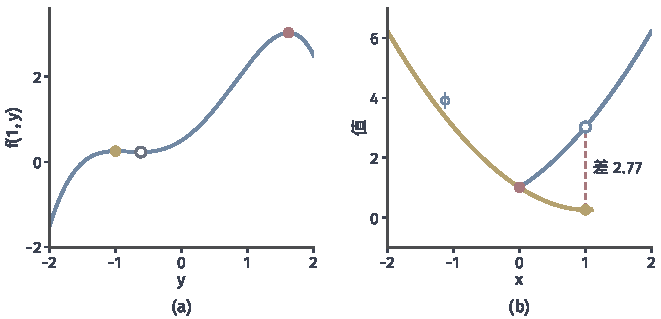
\includegraphics[width=112mm]{figures/05-optimization/07-multiple-criteria-and-nested-optimization/matplotlib/minimax-local-response/figure.pdf}
 \caption{内层不凹的例子，$f=\frac12x^2+xy+y^2-\frac14y^4$，$Y=[-2,2]$。(a)$x=1$时的内层函数：黄点是局部极大，红点是全局极大，空心点是局部极小。(b)蓝线是真实的$\phi$，红点是外层最优解；黄线是沿局部极大分支算得的值。$x=1$处两者相差$2.77$，局部分支到$x\approx1.089$处消失。}
 \label{fig:minimax-local-response}
\end{BookInlineFigure}

假设内层算法从$y<-0.618$的地方起步，它会收敛到$y=-1$。这一步的代价极大：报告的最坏值是$0.25$，真实值是$3.023$。更糟的是外层的方向，$\partial_xf=x+y$在这个响应处是
\[
 \partial_xf(1,-1)=0,
\]
看起来$x=1$已经驻定。而真实的导数是
\[
 \phi'(1)=1+1.618=2.618.
\]
图~\ref{fig:minimax-local-response}(b)中，黄线的局部分支一路下降，到$x=1$处还很低，蓝线的真实$\phi$却在升高。外层最优解其实是$x=0$，$\phi(0)=1$；局部分支报告的$0.25$甚至低于真正的最优值。

内层关于$\bm{y}$凹时，这个问题不存在，因为凹函数在凸集上的局部极大就是全局极大。否则，一个响应的“最优”只是相对于找到它的算法而言，后面报告结果时必须说明这一点。

\subsection{近似响应}
\label{sec:minimax-approx-response}

实际计算很少精确解内层，算到什么程度够用？先定义内层误差。

固定$\bm{x}$，对候选响应$\tilde{\bm{y}}\in\bm{Y}$，称
\begin{equation}
 \varepsilon=\phi(\bm{x})-f(\bm{x},\tilde{\bm{y}})\geq0
 \label{eq:minimax-inner-gap}
\end{equation}
为内层间隙。用它衡量比用$\bm{y}$的距离更合适，因为外层真正关心的是最坏值差多少。要把间隙转成外层梯度的误差，需要一座桥，这座桥就是强凹性：顶部越尖，间隙小就越能说明位置近，如同碗越陡，高度差小，水平距离就越小。

下面的条件贯穿本节。设$\bm{Y}$闭凸；$f$的梯度在$\bm{X}\times\bm{Y}$上$L$-Lipschitz；对每个$\bm{x}$，$f(\bm{x},\cdot)$在$\bm{Y}$上$\mu$强凹，$\mu>0$，记$\kappa=L/\mu$。

\begin{theorem}[内层间隙到外层梯度的传递]
\label{thm:minimax-inexact-gradient}
在上述条件下，内层响应唯一，记为$\bm{y}^\star(\bm{x})$。对任意$\tilde{\bm{y}}\in\bm{Y}$，
\begin{equation}
 \lVert\tilde{\bm{y}}-\bm{y}^\star(\bm{x})\rVert_2\leq\sqrt{\frac{2\varepsilon}{\mu}}.
 \label{eq:minimax-distance}
\end{equation}
进一步，
\begin{equation}
 \bigl\lVert\nabla_{\bm{x}}f(\bm{x},\tilde{\bm{y}})-\nabla_{\bm{x}}f(\bm{x},\bm{y}^\star(\bm{x}))\bigr\rVert_2\leq L\sqrt{\frac{2\varepsilon}{\mu}}.
 \label{eq:minimax-gradient-error}
\end{equation}
\end{theorem}

\begin{proof}
强凹函数在闭凸集上的最大点存在且唯一，记$\bm{y}^\star=\bm{y}^\star(\bm{x})$。最优性给出
\[
 \langle\nabla_{\bm{y}}f(\bm{x},\bm{y}^\star),\tilde{\bm{y}}-\bm{y}^\star\rangle\leq0.
\]
由$\mu$强凹的二次上界，
\[
 f(\bm{x},\tilde{\bm{y}})\leq f(\bm{x},\bm{y}^\star)+\langle\nabla_{\bm{y}}f(\bm{x},\bm{y}^\star),\tilde{\bm{y}}-\bm{y}^\star\rangle-\frac{\mu}{2}\lVert\tilde{\bm{y}}-\bm{y}^\star\rVert_2^2.
\]
把前一式代入，得到
\[
 f(\bm{x},\tilde{\bm{y}})\leq\phi(\bm{x})-\frac{\mu}{2}\lVert\tilde{\bm{y}}-\bm{y}^\star\rVert_2^2.
\]
移项就是式~\eqref{eq:minimax-distance}。再用$\nabla f$的Lipschitz性，就得到式~\eqref{eq:minimax-gradient-error}。
\end{proof}

用$f=-\frac12x^2+2xy-\frac12y^2$在$x=1$处核对，$\mu=1$，$y^\star=2$。取$\tilde{y}=1$，内层值和最坏值分别是
\[
 f(1,1)=1,\qquad\phi(1)=\frac32,
\]
所以$\varepsilon=\frac12$。式~\eqref{eq:minimax-distance}的右端是$1$，真实距离也是$1$，等号成立，因为这个内层函数恰好是二次的。

外层偏导数$\partial_xf=-1+2y$在$\tilde{y}=1$处是$1$，真实导数是$3$，误差是$2$，见图~\ref{fig:minimax-approx-response}。式~\eqref{eq:minimax-gradient-error}用$L=3$给出的上界是$3$，真实误差不超过它。这里交叉项的系数是$2$，把$L$换成$\partial_xf$对$y$的Lipschitz常数$2$，上界就是$2$，恰好等于真实误差。

\begin{BookInlineFigure}
 \centering
 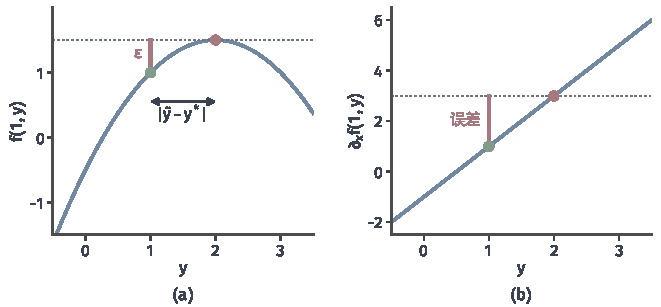
\includegraphics[width=112mm]{figures/05-optimization/07-multiple-criteria-and-nested-optimization/matplotlib/minimax-approx-response/figure.pdf}
 \caption{$f=-\frac12x^2+2xy-\frac12y^2$在$x=1$处。(a)内层函数，红点是最优响应，绿点是候选响应$\tilde{y}=1$，红线是内层间隙$\varepsilon=\frac12$，双箭头是响应距离。(b)外层偏导数关于$y$的直线，红点是真实导数$3$，绿点是候选给出的$1$，红线是误差。}
 \label{fig:minimax-approx-response}
\end{BookInlineFigure}

\paragraph{误差怎样影响外层}
梯度带误差时，外层下降还成立吗？先要知道$\phi$够光滑。下面的引理说明响应随$\bm{x}$平稳移动，从而$\phi$可微且梯度Lipschitz。这里不需要$\bm{Y}$紧。

\begin{lemma}[响应的稳定性与$\phi$的光滑性]
\label{lem:minimax-response-lipschitz}
在上述条件下，设$\bm{X}=\mathbb{R}^n$。则$\bm{y}^\star(\cdot)$是$\kappa$-Lipschitz的，$\phi$可微，梯度仍由式~\eqref{eq:minimax-danskin-gradient}的表达式给出，并且$\nabla\phi$是$L_\phi$-Lipschitz的，其中
\begin{equation}
 L_\phi=L(1+\kappa).
 \label{eq:minimax-phi-smooth}
\end{equation}
\end{lemma}

\begin{proof}
记$\bm{y}_1=\bm{y}^\star(\bm{x}_1)$，$\bm{y}_2=\bm{y}^\star(\bm{x}_2)$。两个最优性条件给出
\[
 \langle\nabla_{\bm{y}}f(\bm{x}_1,\bm{y}_1),\bm{y}_2-\bm{y}_1\rangle\leq0,\qquad\langle\nabla_{\bm{y}}f(\bm{x}_2,\bm{y}_2),\bm{y}_1-\bm{y}_2\rangle\leq0.
\]
$f(\bm{x}_2,\cdot)$的$\mu$强凹性给出
\[
 \mu\lVert\bm{y}_1-\bm{y}_2\rVert_2^2\leq\langle\nabla_{\bm{y}}f(\bm{x}_2,\bm{y}_2)-\nabla_{\bm{y}}f(\bm{x}_2,\bm{y}_1),\bm{y}_1-\bm{y}_2\rangle.
\]

右端含$\nabla_{\bm{y}}f(\bm{x}_2,\bm{y}_2)$的项由第二个最优性条件非正，可以丢掉，于是
\[
 \mu\lVert\bm{y}_1-\bm{y}_2\rVert_2^2\leq-\langle\nabla_{\bm{y}}f(\bm{x}_2,\bm{y}_1),\bm{y}_1-\bm{y}_2\rangle.
\]
在内积中加减$\nabla_{\bm{y}}f(\bm{x}_1,\bm{y}_1)$，并用第一个最优性条件丢掉一项，得到
\[
 \mu\lVert\bm{y}_1-\bm{y}_2\rVert_2^2\leq\langle\nabla_{\bm{y}}f(\bm{x}_1,\bm{y}_1)-\nabla_{\bm{y}}f(\bm{x}_2,\bm{y}_1),\bm{y}_1-\bm{y}_2\rangle.
\]
由Cauchy--Schwarz不等式和Lipschitz条件，得到
\[
 \lVert\bm{y}_1-\bm{y}_2\rVert_2\leq\kappa\lVert\bm{x}_1-\bm{x}_2\rVert_2.
\]

再证可微。任取$\bm{x}$和$\bm{d}$，记$\bm{y}=\bm{y}^\star(\bm{x})$，$\bm{y}_{\bm{d}}=\bm{y}^\star(\bm{x}+\bm{d})$，$\bm{g}=\nabla_{\bm{x}}f(\bm{x},\bm{y})$。用$\bm{y}$在$\bm{x}+\bm{d}$处的值作下界，并由光滑性，
\[
 \phi(\bm{x}+\bm{d})-\phi(\bm{x})\geq f(\bm{x}+\bm{d},\bm{y})-f(\bm{x},\bm{y})\geq\langle\bm{g},\bm{d}\rangle-\frac{L}{2}\lVert\bm{d}\rVert_2^2.
\]

用$\bm{y}_{\bm{d}}$作上界，同样由光滑性和响应的Lipschitz性，
\[
 \begin{aligned}
 \phi(\bm{x}+\bm{d})-\phi(\bm{x})&\leq f(\bm{x}+\bm{d},\bm{y}_{\bm{d}})-f(\bm{x},\bm{y}_{\bm{d}})\\
 &\leq\langle\nabla_{\bm{x}}f(\bm{x},\bm{y}_{\bm{d}}),\bm{d}\rangle+\frac{L}{2}\lVert\bm{d}\rVert_2^2\\
 &\leq\langle\bm{g},\bm{d}\rangle+L\kappa\lVert\bm{d}\rVert_2^2+\frac{L}{2}\lVert\bm{d}\rVert_2^2.
 \end{aligned}
\]
上下夹逼，得到$\phi$可微且梯度为$\bm{g}$。

最后，由梯度公式和响应的Lipschitz性，
\[
 \lVert\nabla\phi(\bm{x}_1)-\nabla\phi(\bm{x}_2)\rVert_2\leq L\lVert\bm{x}_1-\bm{x}_2\rVert_2+L\lVert\bm{y}_1-\bm{y}_2\rVert_2\leq L(1+\kappa)\lVert\bm{x}_1-\bm{x}_2\rVert_2.
\]
\end{proof}

式~\eqref{eq:minimax-phi-smooth}说明，$\phi$的光滑常数可能比$f$大$\kappa$倍。原因是响应会跟着$\bm{x}$动，$\kappa$越大响应动得越快，外层看到的函数越弯。

\begin{theorem}[带内层误差的外层下降]
\label{thm:minimax-inexact-descent}
在引理~\ref{lem:minimax-response-lipschitz}的条件下，设$\phi$有下界$\phi_{\inf}$，外层迭代$\bm{x}^{(t+1)}=\bm{x}^{(t)}-\alpha\bm{g}^{(t)}$，其中$0<\alpha\leq1/L_\phi$，$\bm{g}^{(t)}$与$\nabla\phi(\bm{x}^{(t)})$之差的范数不超过$\delta$。则
\begin{equation}
 \min_{0\leq t<T}\lVert\nabla\phi(\bm{x}^{(t)})\rVert_2^2\leq\frac{2(\phi(\bm{x}^{(0)})-\phi_{\inf})}{\alpha T}+\delta^2.
 \label{eq:minimax-inexact-descent}
\end{equation}
\end{theorem}

\begin{proof}
记$\bm{x}=\bm{x}^{(t)}$，$\bm{g}=\bm{g}^{(t)}$，$\bm{e}=\bm{g}-\nabla\phi(\bm{x})$。由$L_\phi$-光滑的下降引理和$\alpha L_\phi\leq1$，
\[
 \phi(\bm{x}^{(t+1)})\leq\phi(\bm{x})-\alpha\langle\nabla\phi(\bm{x}),\bm{g}\rangle+\frac{\alpha}{2}\lVert\bm{g}\rVert_2^2.
\]
对任意向量$\bm{a},\bm{b}$有恒等式
\[
 -\langle\bm{a},\bm{b}\rangle+\frac12\lVert\bm{b}\rVert_2^2=\frac12\lVert\bm{b}-\bm{a}\rVert_2^2-\frac12\lVert\bm{a}\rVert_2^2.
\]
取$\bm{a}=\nabla\phi(\bm{x})$，$\bm{b}=\bm{g}$，得到
\[
 \phi(\bm{x}^{(t+1)})\leq\phi(\bm{x})-\frac{\alpha}{2}\lVert\nabla\phi(\bm{x})\rVert_2^2+\frac{\alpha}{2}\lVert\bm{e}\rVert_2^2.
\]
对$t=0,\ldots,T-1$求和，用$\phi(\bm{x}^{(T)})\geq\phi_{\inf}$和$\lVert\bm{e}\rVert_2\leq\delta$，再除以$\alpha T/2$，左端的平均不小于最小值，即得结论。
\end{proof}

式~\eqref{eq:minimax-inexact-descent}有两项：第一项随$T$下降，第二项是内层误差留下的平台。要让外层梯度小到$\epsilon$，内层误差$\delta$也要到$\epsilon$量级。结合式~\eqref{eq:minimax-gradient-error}，这要求内层间隙满足$L\sqrt{2\varepsilon/\mu}\lesssim\epsilon$，即$\varepsilon$是$\mu\epsilon^2/L^2$量级。

\paragraph{计算过程}
内层用$K$步投影梯度上升，并从上一轮的响应出发，比从头开始省事，因为$\bm{x}$变化不大时响应也变化不大。仍用$f=-\frac12x^2+2xy-\frac12y^2$。

\needspace{6\baselineskip}
\paragraph{变量}
\begin{itemize}
 \item $x^{(t)}$：外层变量；
 \item $y^{(t)}$：第$t$轮内层结束后的近似响应；
 \item $K$：每轮内层步数；$\beta$：内层步长；$\alpha$：外层步长。
\end{itemize}

\paragraph{初始化}
取$x^{(0)}$和$y^{(-1)}$。例中$x^{(0)}=1$，$y^{(-1)}=0$，$K=2$，$\beta=\frac12$，$\alpha=\frac16$。内层的曲率是$1$，步长$\beta=\frac12$不超过曲率的倒数。

\needspace{6\baselineskip}
\paragraph{每轮更新}
\begin{enumerate}
 \item 从$y=y^{(t-1)}$出发做$K$次内层更新$y\leftarrow P_Y(y+\beta\partial_yf(x^{(t)},y))$，得$y^{(t)}$。例中$\partial_yf=2x-y$，第一轮
 \[
  y:\ 0\to0+\frac12\cdot2=1\to1+\frac12\cdot1=1.5,\qquad y^{(0)}=1.5.
 \]
 \item 用当前响应计算外层偏导数$g^{(t)}=\partial_xf(x^{(t)},y^{(t)})$。例中第一轮
 \[
  g^{(0)}=-1+2\cdot1.5=2.
 \]
 \item 更新外层$x^{(t+1)}=x^{(t)}-\alpha g^{(t)}$。例中第一轮
 \[
  x^{(1)}=1-\frac26=\frac23.
 \]
\end{enumerate}

第二轮内层从$y=1.5$出发，目标$2x^{(1)}=\frac43$，两步给出
\[
 y:\ 1.5\to1.41667\to1.375,\qquad y^{(1)}=1.375.
\]
外层偏导数是$g^{(1)}=-\frac23+2.75\approx2.0833$，所以$x^{(2)}\approx0.3194$。真实导数$3x^{(1)}=2$，这一轮的误差约为$0.083$。

第一轮的真实导数是$3$，误差是$1$；第二轮暖启动之后，误差降到$0.083$。迭代继续下去，到设定的外层梯度精度为止。这里用$\lvert g^{(t)}\rvert$作判据时要记住，它自身带有内层误差。

\paragraph{一般非凹内层}
上面的传递依赖强凹性。没有强凹性时，$\nabla_{\bm{y}}f$很小不说明响应接近最优。式~\eqref{eq:minimax-nonconcave}中$(x,y)=(1,-1)$的内层梯度严格为零，内层间隙却是$2.77$。此时只从$\tilde{\bm{y}}$算出的值只是$\phi(\bm{x})$的下界，真实误差不可知，外层停止时必须说明实际使用的响应证据：用了什么内层算法、多少起点、最后的残差，而不能把$\nabla_{\bm{y}}f\approx\bm{0}$说成“内层已解”。

\section{下降—上升方法}
\label{sec:minimax-gda}

内层响应法每轮都要解一个优化问题，代价不小。能不能每轮只算一次两侧的梯度，让$\bm{x}$走一小步下山，同时让$\bm{y}$走一小步上山？本节研究这个最便宜的做法，它在什么情况下行得通，在什么情况下行不通。

\paragraph{主要思想}
设$\bm{X},\bm{Y}$是闭凸集，$f$可微。不再要求内层解到最优，而是让$\bm{y}$只沿内层目标的梯度走一步，$\bm{x}$沿外层方向走一步。这样的方法称为\term{梯度下降—上升}（gradient descent--ascent，GDA）。

两个偏梯度都在旧点计算，称为同时更新：
\begin{equation}
 \begin{aligned}
 \bm{x}^{(t+1)}&=P_{\bm{X}}\bigl(\bm{x}^{(t)}-\alpha\nabla_{\bm{x}}f(\bm{x}^{(t)},\bm{y}^{(t)})\bigr),\\
 \bm{y}^{(t+1)}&=P_{\bm{Y}}\bigl(\bm{y}^{(t)}+\beta\nabla_{\bm{y}}f(\bm{x}^{(t)},\bm{y}^{(t)})\bigr).
 \end{aligned}
 \label{eq:minimax-gda-sim}
\end{equation}

先更新$\bm{x}$，再用新的$\bm{x}$算$\bm{y}$的梯度，称为先后更新：
\begin{equation}
 \begin{aligned}
 \bm{x}^{(t+1)}&=P_{\bm{X}}\bigl(\bm{x}^{(t)}-\alpha\nabla_{\bm{x}}f(\bm{x}^{(t)},\bm{y}^{(t)})\bigr),\\
 \bm{y}^{(t+1)}&=P_{\bm{Y}}\bigl(\bm{y}^{(t)}+\beta\nabla_{\bm{y}}f(\bm{x}^{(t+1)},\bm{y}^{(t)})\bigr).
 \end{aligned}
 \label{eq:minimax-gda-alt}
\end{equation}

两式只有第二行里$\bm{x}$的上标不同，却是不同的递推，下面的例子里轨迹的性质也不同。比较时必须说明用的是哪一种。

\paragraph{计算过程}
用$f(x,y)=xy$，$X=Y=\mathbb{R}$，唯一鞍点是原点。

\needspace{6\baselineskip}
\paragraph{变量}
\begin{itemize}
 \item $x^{(t)},y^{(t)}$：两组变量；
 \item $\alpha,\beta>0$：两侧步长。
\end{itemize}

\paragraph{初始化}
取$(x^{(0)},y^{(0)})$。例中$(x^{(0)},y^{(0)})=(1,0)$，$\alpha=\beta=\frac12$。

\needspace{6\baselineskip}
\paragraph{每轮更新}
\begin{enumerate}
 \item 计算两个偏导数。例中$\partial_xf=y$，$\partial_yf=x$。
 \item 按式~\eqref{eq:minimax-gda-sim}或式~\eqref{eq:minimax-gda-alt}更新。例中同时更新的第一轮
 \[
  x^{(1)}=1-\frac12\cdot0=1,\qquad y^{(1)}=0+\frac12\cdot1=\frac12.
 \]
 第二轮、第三轮分别得到
 \[
  (x^{(2)},y^{(2)})=(0.75,1),\qquad(x^{(3)},y^{(3)})=(0.25,1.375).
 \]
 \item 先后更新的第一轮结果相同，因为$y^{(0)}=0$时$x$不动。第二轮和第三轮分别是
 \[
  (x^{(2)},y^{(2)})=(0.75,0.875),\qquad(x^{(3)},y^{(3)})=(0.3125,1.03125).
 \]
\end{enumerate}

通常的结束条件是步数达到上限，或残差小于容差。例中距离鞍点的平方，同时更新依次为$1,1.25,1.5625,1.953$，每轮乘以$1.25$；先后更新依次为$1,1.25,1.3281,1.161$，有界地上下波动。最终两种更新都没有接近鞍点。下一小节解释原因。

\subsection{旋转现象}
\label{sec:minimax-rotation}

把同时更新用矩阵写出来，记$\bm{z}=(x,y)^\top$，式~\eqref{eq:minimax-gda-sim}成为
\begin{equation}
 \bm{z}^{(t+1)}=\begin{pmatrix}1&-\alpha\\\alpha&1\end{pmatrix}\bm{z}^{(t)}.
 \label{eq:minimax-gda-matrix}
\end{equation}

这个矩阵是一个旋转矩阵乘以$\sqrt{1+\alpha^2}$。两列互相正交，长度都是$\sqrt{1+\alpha^2}$，所以
\begin{equation}
 \lVert\bm{z}^{(t+1)}\rVert_2^2=(1+\alpha^2)\lVert\bm{z}^{(t)}\rVert_2^2.
 \label{eq:minimax-gda-growth}
\end{equation}

对任何固定的$\alpha>0$，距离都按几何级数增长。$\alpha=\frac12$时每轮乘以$1.25$，与上面的数字一致。步长取得再小，也只是增长得慢，不会变成收缩。

几何上，迭代方向是$(-y,x)$，它和位置向量$(x,y)$处处垂直，也就是沿着以原点为圆心的圆的切线方向。沿切线走一小段，总是落到更大的圆上。这像绕着一个圆运动的人每走一步都沿当前切线走直线，路线不是回到原圆，而是向外盘旋。连续时间的方程$\dot{\bm{z}}=(-y,x)$恰好沿圆运动，半径不变；离散化把这个“恰好不靠近”的运动变成了发散。

先后更新的矩阵是
\[
 \begin{pmatrix}1&-\alpha\\\alpha&1-\alpha^2\end{pmatrix},
\]
行列式是$1$，迹是$2-\alpha^2$。$0<\alpha<2$时迹的绝对值小于$2$，两个特征值是模为$1$的共轭复数，迭代既不发散也不收敛。

这一点可以用一个守恒量看得更清楚。令$Q=x^2+y^2-\alpha xy$，记$x^{+}=x-\alpha y$，$y^{+}=y+\alpha x^{+}$。先处理含$y^{+}$的两项：
\[
 (y^{+})^2-\alpha x^{+}y^{+}=y^{+}(y^{+}-\alpha x^{+})=y^{+}y=y^2+\alpha x^{+}y.
\]
再处理剩下的项：
\[
 (x^{+})^2+\alpha x^{+}y=x^{+}(x^{+}+\alpha y)=x^{+}x=x^2-\alpha xy.
\]
两式相加，得到
\[
 (x^{+})^2+(y^{+})^2-\alpha x^{+}y^{+}=x^2+y^2-\alpha xy,
\]
所以$Q$沿迭代不变。$0<\alpha<2$时$Q$是正定二次型，迭代点永远留在同一个椭圆上，既跑不掉也到不了中心。图~\ref{fig:minimax-gda-rotation}(a)(b)画出了两种轨迹。

\begin{BookInlineFigure}
 \centering
 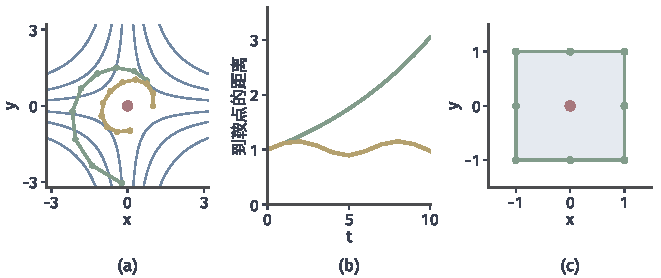
\includegraphics[width=112mm]{figures/05-optimization/07-multiple-criteria-and-nested-optimization/matplotlib/minimax-gda-rotation/figure.pdf}
 \caption{$f=xy$上的下降—上升，蓝线是等高线，红点是鞍点。(a)$\alpha=\frac12$，起点$(1,0)$，$10$步：绿色是同时更新，向外盘旋；黄色是先后更新，留在椭圆上。(b)两种更新到鞍点的距离。(c)盒子$[-1,1]^2$上的投影同时更新，$\alpha=1$，从$(1,0)$出发，$8$步回到起点。}
 \label{fig:minimax-gda-rotation}
\end{BookInlineFigure}

\paragraph{加上约束也不收敛}
把迭代限制在盒子里能防止发散，却不能让它停在鞍点。取$X=Y=[-1,1]$，$\alpha=\beta=1$，从$(1,0)$出发做投影同时更新，投影就是逐分量截断到$[-1,1]$。第一步$x=1-0=1$，$y=0+1=1$；第二步$x=1-1=0$，$y=1+1=2$，截断成$1$。继续算下去，得到
\[
 \begin{aligned}
 (1,0)&\to(1,1)\to(0,1)\to(-1,1)\to(-1,0)\\
 &\to(-1,-1)\to(0,-1)\to(1,-1)\to(1,0).
 \end{aligned}
\]

八步之后回到起点，见图~\ref{fig:minimax-gda-rotation}(c)。由式~\eqref{eq:minimax-box-gap}，循环上的间隙$\lvert x\rvert+\lvert y\rvert$取$1$或$2$，永远不小于$1$。定理~\ref{thm:minimax-theorem}的条件全部满足，鞍点存在，算法却找不到它。存在性定理回答解在不在，不回答某个算法能否到达。

\paragraph{只看一侧的数不足以判断}
图~\ref{fig:minimax-gda-monitor}(a)是同时更新过程中$f(x^{(t)},y^{(t)})$的值。从$t=2$到$t=5$，它从$0.75$一路降到$-1.52$。如果只看这条线，会以为外层目标在稳步下降，而图~\ref{fig:minimax-gda-monitor}(b)显示点正在远离解。$f$的值本来就该由一侧压低、另一侧抬高，它的升降不说明任何问题。

\begin{BookInlineFigure}
 \centering
 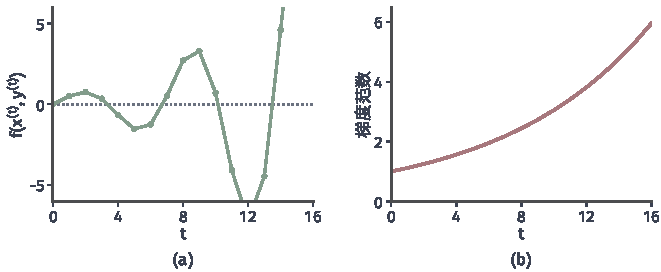
\includegraphics[width=112mm]{figures/05-optimization/07-multiple-criteria-and-nested-optimization/matplotlib/minimax-gda-monitor/figure.pdf}
 \caption{$f=xy$上同时更新的监控量，$\alpha=\frac12$，起点$(1,0)$。(a)绿线是代价$f$的值，在部分时段连续下降，又在更大的幅度上振荡。(b)红线是两侧梯度的范数$\lVert(y,-x)\rVert_2$，它等于到鞍点的距离，持续增长。}
 \label{fig:minimax-gda-monitor}
\end{BookInlineFigure}

反过来，梯度为零也说明不了稳定。对$f=xy$，原点两侧梯度都为零，而且原点就是解，迭代却从任何非零点开始都远离它，一旦有扰动也回不去。对$f=y^2-x^2$，原点两侧梯度也为零，但迭代$x^{+}=(1+2\alpha)x$，$y^{+}=(1+2\alpha)y$从原点附近往外推，原点又不是解。所以驻定只回答“这个点本身怎样”，不回答“迭代会不会留在它附近”，后者要看迭代映射的线性化。

\subsection{响应速度}
\label{sec:minimax-speed}

$f=xy$没有内层曲率，$\bm{y}$没有自己想去的位置。内层有强凹性时，$\bm{y}$就有一个目标$\bm{y}^\star(\bm{x})$，问题变成：$\bm{y}$能否跟上这个随$\bm{x}$移动的目标？

继续用$f=-\frac12x^2+2xy-\frac12y^2$，最优响应是$y=2x$，原点是顺序问题的解。令$\beta=r\alpha$，$r$是两侧步长之比。迭代$\bm{z}^{+}=(\bm{I}-\alpha\bm{J}_r)\bm{z}$的矩阵是
\begin{equation}
 \bm{J}_r=\begin{pmatrix}-1&2\\-2r&r\end{pmatrix}.
 \label{eq:minimax-timescale-matrix}
\end{equation}

$\bm{J}_r$的迹是$r-1$，行列式是$3r$。当$1<r<13$时，判别式$(r-1)^2-12r<0$，两个特征值是共轭复数$\lambda$，满足$\operatorname{Re}\lambda=\frac{r-1}{2}$，$\lvert\lambda\rvert^2=3r$。迭代的模平方是
\[
 \lvert1-\alpha\lambda\rvert^2=1-\alpha(r-1)+3r\alpha^2.
\]

这个量小于$1$，当且仅当
\begin{equation}
 0<\alpha<\frac{r-1}{3r}.
 \label{eq:minimax-timescale-stable}
\end{equation}

$r=1$时模平方是$1+3\alpha^2>1$，任何步长都发散。$r<1$时两个特征值的实部为负，$\lvert1-\alpha\lambda\rvert>1$，同样发散。$r=4$时条件是$\alpha<\frac14$，例如$\alpha=0.1$时模平方是$0.82$。两种选择用同样的$\alpha$，差别只在$y$走得快不快，见图~\ref{fig:minimax-timescale}。

\begin{BookInlineFigure}
 \centering
 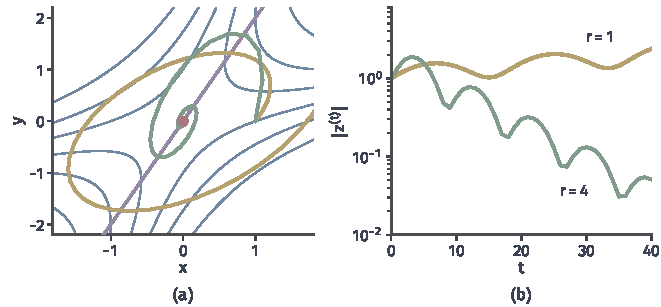
\includegraphics[width=112mm]{figures/05-optimization/07-multiple-criteria-and-nested-optimization/matplotlib/minimax-timescale/figure.pdf}
 \caption{$f=-\frac12x^2+2xy-\frac12y^2$上的同时更新，$\alpha=0.1$，起点$(1,0)$，$40$步。蓝线是等高线，紫线是最优响应$y=2x$，红点是解。黄线$r=1$，两侧同速，$y$跟不上$x$，轨迹向外盘旋。绿线$r=4$，$y$走得快，轨迹贴着紫线向解收敛。(b)到解的距离。}
 \label{fig:minimax-timescale}
\end{BookInlineFigure}

$r$的门槛来自$f$的结构。$\partial_x^2f=-1$是外层变量的负曲率，$\partial_y^2f=-1$是内层变量提供的强凹性。外层独自运动时是往外推的，只有$y$足够快地跟上$y=2x$，外层才看得到$\phi''=3>0$的正曲率。$y$落后时，外层感受到的是$f$在旧$y$上的负曲率，于是被推开。

\paragraph{跟踪误差的递推}
一般情形可以用跟踪误差来刻画这种竞赛。沿用第~\ref{sec:minimax-approx-response}节的条件，记跟踪误差为
\begin{equation}
 e_t=\lVert\bm{y}^{(t)}-\bm{y}^\star(\bm{x}^{(t)})\rVert_2.
 \label{eq:minimax-tracking-error}
\end{equation}

第~\ref{chap:feasible-iterations}章证明过：$\mu$强凸、$L$-光滑的函数上，步长为$1/L$的投影梯度法把到解的距离至少缩小到$\rho=\sqrt{1-\mu/L}$倍。把它用到凸函数$-f(\bm{x},\cdot)$上。

\begin{lemma}[跟踪误差的递推]
\label{lem:minimax-tracking}
设$\bm{x}^{(t+1)}$已经算出，从$\bm{y}^{(t)}$出发在$f(\bm{x}^{(t+1)},\cdot)$上做$K$步步长$1/L$的投影梯度上升，得到$\bm{y}^{(t+1)}$。则
\begin{equation}
 e_{t+1}\leq\rho^{K}\bigl(e_t+\kappa\lVert\bm{x}^{(t+1)}-\bm{x}^{(t)}\rVert_2\bigr).
 \label{eq:minimax-tracking}
\end{equation}
\end{lemma}

\begin{proof}
$K$步投影梯度上升的收缩给出
\[
 e_{t+1}\leq\rho^K\lVert\bm{y}^{(t)}-\bm{y}^\star(\bm{x}^{(t+1)})\rVert_2.
\]
用三角不等式，并由引理~\ref{lem:minimax-response-lipschitz}的$\kappa$-Lipschitz性，
\[
 \lVert\bm{y}^{(t)}-\bm{y}^\star(\bm{x}^{(t+1)})\rVert_2\leq e_t+\kappa\lVert\bm{x}^{(t+1)}-\bm{x}^{(t)}\rVert_2.
\]
两式合起来即得。
\end{proof}

式~\eqref{eq:minimax-tracking}里，$\rho^K$是内层追赶的速度，$\kappa\lVert\bm{x}^{(t+1)}-\bm{x}^{(t)}\rVert_2$是目标跑开的距离。要跟得上，有两种办法：增加$K$，或者减小外层步长。

取$K=1$，看外层步长要小到什么程度。设每步外层移动量是$\alpha\lVert\bm{g}\rVert_2$，$\rho\approx1-\frac{1}{2\kappa}$。递推的稳态是
\[
 e_\infty\approx\frac{\kappa\alpha\lVert\bm{g}\rVert_2}{1-\rho}\approx2\kappa^2\alpha\lVert\bm{g}\rVert_2.
\]

外层梯度的误差约为$Le_\infty$。要让它不超过$\frac12\lVert\bm{g}\rVert_2$，需要$\alpha\lesssim\frac{1}{4\kappa^2L}$，也就是$\alpha/\beta$是$1/\kappa^2$量级。这个推算只是说明量级，不是证明。完整的结论要把式~\eqref{eq:minimax-tracking}和定理~\ref{thm:minimax-inexact-descent}放进同一个势函数，得到的是非凸—强凹问题上求$\phi$的$\epsilon$驻定点需要$O(\kappa^2/\epsilon^2)$量级的梯度读取。该证明篇幅较长，读者可查阅双时间尺度下降—上升的专门分析。

理论的步长是保守的。上例$L=3$，$\kappa=3$，上述量级给出的$\alpha$约为$\frac{1}{108}$，而取$\beta=\frac13$时由式~\eqref{eq:minimax-timescale-stable}可算出实际的稳定范围到$\alpha<\frac16$。保证覆盖的是一个函数类中最差的情形，这与第~\ref{chap:first-order-methods}章步长的保守取法一样。

\paragraph{非凸—非凹情形}
以上依赖强凹性带来的$\kappa$-Lipschitz响应。式~\eqref{eq:minimax-nonconcave}中最优响应在$x=0$处从$-\sqrt2$跳到$\sqrt2$，没有任何Lipschitz常数，内层再快也不能平稳地跟踪。此时必须分别说明三件事：用的是什么步长组合，内层响应求到了什么程度，所报告的驻定概念是什么，第~\ref{sec:minimax-evaluation}节回到这些问题。一般非凸—非凹问题上，下降—上升可能循环，也可能发散，没有与上面同类的保证。

\section{校正方向}
\label{sec:minimax-correction}

上一节的失败发生在凸凹问题上，而且鞍点存在。所以问题不在问题本身，在迭代格式。本节先把鞍点条件写成统一的形式，看清旋转是从哪里来的，再修改迭代，用另一处的方向校正当前一步。

\paragraph{变分不等式形式}
把两组变量合并，记$\bm{z}=(\bm{x},\bm{y})$，$\bm{Z}=\bm{X}\times\bm{Y}$，定义
\begin{equation}
 \bm{F}(\bm{z})=\begin{pmatrix}\nabla_{\bm{x}}f(\bm{x},\bm{y})\\-\nabla_{\bm{y}}f(\bm{x},\bm{y})\end{pmatrix}.
 \label{eq:minimax-operator}
\end{equation}

两侧步长相同时，同时更新就是
\[
 \bm{z}^{+}=P_{\bm{Z}}\bigl(\bm{z}-\alpha\bm{F}(\bm{z})\bigr).
\]

它和投影梯度法外形一样，但$\bm{F}$一般不是任何函数的梯度。鞍点条件也能用$\bm{F}$写出来，这个写法就是第~\ref{chap:constrained-optimality}章见过的变分不等式。

\begin{theorem}[鞍点的变分不等式刻画]
\label{thm:minimax-vi}
设$\bm{X},\bm{Y}$非空闭凸，$f$在含$\bm{Z}$的开集上可微，关于$\bm{x}$凸，关于$\bm{y}$凹。则$\bm{z}^\star\in\bm{Z}$是全局鞍点，当且仅当
\begin{equation}
 \langle\bm{F}(\bm{z}^\star),\bm{z}-\bm{z}^\star\rangle\geq0\qquad\text{对所有}\ \bm{z}\in\bm{Z}.
 \label{eq:minimax-vi}
\end{equation}
\end{theorem}

\begin{proof}
记$\bm{z}^\star=(\bm{x}^\star,\bm{y}^\star)$。设它是鞍点。$\bm{x}^\star$在凸集$\bm{X}$上最小化可微凸函数$f(\cdot,\bm{y}^\star)$，一阶条件给出
\[
 \langle\nabla_{\bm{x}}f(\bm{z}^\star),\bm{x}-\bm{x}^\star\rangle\geq0.
\]
$\bm{y}^\star$在$\bm{Y}$上最大化凹函数$f(\bm{x}^\star,\cdot)$，一阶条件给出
\[
 \langle-\nabla_{\bm{y}}f(\bm{z}^\star),\bm{y}-\bm{y}^\star\rangle\geq0.
\]
两式相加即为式~\eqref{eq:minimax-vi}。

反过来，在式~\eqref{eq:minimax-vi}中取$\bm{z}=(\bm{x},\bm{y}^\star)$，得到上面第一式，由凸性，$\bm{x}^\star$是$f(\cdot,\bm{y}^\star)$的全局最小点。取$\bm{z}=(\bm{x}^\star,\bm{y})$，得到第二式，由凹性，$\bm{y}^\star$是$f(\bm{x}^\star,\cdot)$的全局最大点。这就是式~\eqref{eq:minimax-saddle}。
\end{proof}

式~\eqref{eq:minimax-vi}的几何含义是，从$\bm{z}^\star$看向任何可行方向，它与$\bm{F}(\bm{z}^\star)$的夹角都不超过直角，见图~\ref{fig:minimax-vi-geometry}。

\begin{BookInlineFigure}
 \centering
 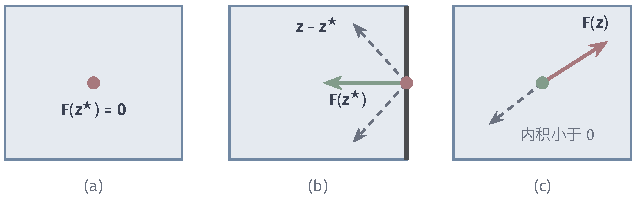
\includegraphics[width=107.7mm]{figures/05-optimization/07-multiple-criteria-and-nested-optimization/tikz/minimax-vi-geometry/figure.pdf}
 \caption{变分不等式的几何。浅蓝矩形是$\bm{Z}$。(a)解在内部时$\bm{F}(\bm{z}^\star)=\bm{0}$。(b)解在边界（深灰粗线）上时$\bm{F}(\bm{z}^\star)$指向内部，虚线表示的可行方向$\bm{z}-\bm{z}^\star$都与它成锐角。(c)绿点不是解，存在可行方向与红色的$\bm{F}(\bm{z})$内积为负。}
 \label{fig:minimax-vi-geometry}
\end{BookInlineFigure}

$\bm{F}$的性质由凸凹性决定。

\begin{lemma}[单调性]
\label{lem:minimax-monotone}
在定理~\ref{thm:minimax-vi}的条件下，$\bm{F}$是\term{单调算子}（monotone operator），即对任意$\bm{z}_1,\bm{z}_2\in\bm{Z}$，
\begin{equation}
 \langle\bm{F}(\bm{z}_1)-\bm{F}(\bm{z}_2),\bm{z}_1-\bm{z}_2\rangle\geq0.
 \label{eq:minimax-monotone}
\end{equation}
\end{lemma}

\begin{proof}
记$\bm{z}_i=(\bm{x}_i,\bm{y}_i)$。由$f(\cdot,\bm{y}_1)$和$f(\cdot,\bm{y}_2)$的凸性，
\[
 \begin{aligned}
 f(\bm{x}_2,\bm{y}_1)&\geq f(\bm{x}_1,\bm{y}_1)+\langle\nabla_{\bm{x}}f(\bm{z}_1),\bm{x}_2-\bm{x}_1\rangle,\\
 f(\bm{x}_1,\bm{y}_2)&\geq f(\bm{x}_2,\bm{y}_2)+\langle\nabla_{\bm{x}}f(\bm{z}_2),\bm{x}_1-\bm{x}_2\rangle.
 \end{aligned}
\]
由$f(\bm{x}_1,\cdot)$和$f(\bm{x}_2,\cdot)$的凹性，
\[
 \begin{aligned}
 f(\bm{x}_1,\bm{y}_2)&\leq f(\bm{x}_1,\bm{y}_1)+\langle\nabla_{\bm{y}}f(\bm{z}_1),\bm{y}_2-\bm{y}_1\rangle,\\
 f(\bm{x}_2,\bm{y}_1)&\leq f(\bm{x}_2,\bm{y}_2)+\langle\nabla_{\bm{y}}f(\bm{z}_2),\bm{y}_1-\bm{y}_2\rangle.
 \end{aligned}
\]
把四个不等式相加，函数值全部相消，整理即得式~\eqref{eq:minimax-monotone}。
\end{proof}

单调是梯度单调的推广，$f$是凸函数时$\nabla f$单调。差别在于$\bm{F}$的Jacobian不对称。$f$二阶可微时，
\[
 \bm{J}=\begin{pmatrix}\nabla^2_{\bm{x}\bm{x}}f&\nabla^2_{\bm{x}\bm{y}}f\\-\nabla^2_{\bm{y}\bm{x}}f&-\nabla^2_{\bm{y}\bm{y}}f\end{pmatrix}.
\]

对角块由凸凹性是半正定的，贡献朝向解的收缩。非对角块反对称，贡献的是旋转，它对$\langle\bm{F}(\bm{z})-\bm{F}(\bm{z}'),\bm{z}-\bm{z}'\rangle$的贡献恰好是零。$f=xy$时对角块全是零，$\bm{J}$只剩反对称部分，所以$\langle\bm{F}(\bm{z}),\bm{z}\rangle=0$。单调性在这里只说明方向不朝外，并不提供任何朝向解的分量，这就是旋转现象的代数来源。

\paragraph{校正的想法}
旋转场里，当前点的方向用一整步就过时了，走到新位置时场已经转了角度。一个自然的修补是：先试探着走一步，读取试探点处的方向，再回到原来的位置，用这个方向走一步。下面的表把这个想法和几种看起来相近的技巧放在一起。

\begin{BookInlineTable}
 \centering
 \begin{tabular}{@{}lll@{}}
  \toprule
  技巧 & 改的是什么 & 对$f=xy$的效果\\
  \midrule
  重球动量 & 叠加上一步的位移 & 把切向位移加强，更快发散\\
  乘子法 & 改目标，加增广项后解内层 & 需要解子问题\\
  外梯度 & 方向取自预测点 & 收缩\\
  乐观梯度 & 用方向的差分校正 & 收缩\\
  \bottomrule
 \end{tabular}
 \caption{几种修改迭代或目标的办法。前两种不是校正方向。}
 \label{tab:minimax-correction-compare}
\end{BookInlineTable}

重球法是第~\ref{chap:first-order-methods}章的单目标加速，叠加的是位置差$\bm{z}^{(t)}-\bm{z}^{(t-1)}$。在$f=xy$上，上一步的位移本身就是切向的，叠加之后向外偏得更多。取$\alpha=0.2$，动量系数$0.5$，迭代的谱半径是$1.125$，比不加动量时的$1.020$还大。

第~\ref{chap:penalty-multiplier-methods}章的乘子法也交替更新原变量和乘子，但它在$\bm{x}$上解一个增广Lagrange子问题，增广项改变了目标。校正方向不改$f$，只改读取方向的位置，每轮仍只是读取几次方向。

\subsection{外梯度法}
\label{sec:minimax-extragradient}

\paragraph{主要思想}
\term{外梯度法}（extragradient method，EG）每轮读取两次方向\scite{korpelevich1976}。先从当前点走一个试探步，读取新方向，再回到当前点，用新方向完成校正：
\begin{equation}
 \begin{aligned}
 \tilde{\bm{z}}^{(t)}&=P_{\bm{Z}}\bigl(\bm{z}^{(t)}-\alpha\bm{F}(\bm{z}^{(t)})\bigr),\\
 \bm{z}^{(t+1)}&=P_{\bm{Z}}\bigl(\bm{z}^{(t)}-\alpha\bm{F}(\tilde{\bm{z}}^{(t)})\bigr).
 \end{aligned}
 \label{eq:minimax-eg}
\end{equation}

校正步的起点仍是$\bm{z}^{(t)}$，只是方向换成了试探点的方向。这和连续做两次普通梯度步不同，后者的第二步从$\tilde{\bm{z}}^{(t)}$出发。

为什么这样能收缩？看$f=xy$，$\bm{F}(x,y)=(y,-x)$。在图~\ref{fig:minimax-eg-step}中，从$\bm{z}$沿切线走到$\tilde{\bm{z}}$，那里的方向已经向内转过了一个角度。把这个方向拿回$\bm{z}$，迈出的一步就略微朝向圆内，抵消了切线外漂。

\begin{BookInlineFigure}
 \centering
 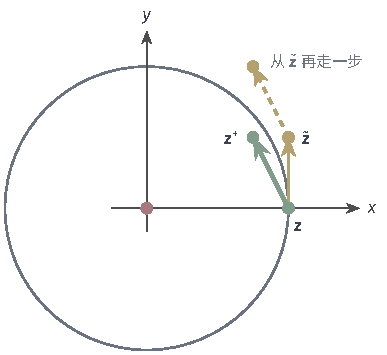
\includegraphics[width=65.6mm]{figures/05-optimization/07-multiple-criteria-and-nested-optimization/tikz/minimax-eg-step/figure.pdf}
 \caption{外梯度的一步，$f=xy$，$\alpha=\frac12$。灰色圆是过$\bm{z}=(1,0)$的等距圆，红点是鞍点。黄色实线箭头走到试探点$\tilde{\bm{z}}=(1,0.5)$，绿色箭头从$\bm{z}$沿试探点的方向走到$\bm{z}^{+}=(0.75,0.5)$，落在圆内。黄色虚线是从试探点再走一步普通梯度步，到$(0.75,1)$，落在圆外。}
 \label{fig:minimax-eg-step}
\end{BookInlineFigure}

代数上，把$\bm{F}(\bm{z})=\bm{A}\bm{z}$代入，$\bm{A}=\begin{pmatrix}0&1\\-1&0\end{pmatrix}$，得到
\[
 \bm{z}^{+}=\bm{z}-\alpha\bm{A}(\bm{z}-\alpha\bm{A}\bm{z})=\bigl(\bm{I}-\alpha\bm{A}+\alpha^2\bm{A}^2\bigr)\bm{z}.
\]

由于$\bm{A}^2=-\bm{I}$，上式成为$\bm{z}^{+}=(1-\alpha^2)\bm{z}-\alpha\bm{A}\bm{z}$。$\bm{z}$与$\bm{A}\bm{z}$正交，长度相同，所以
\begin{equation}
 \lVert\bm{z}^{+}\rVert_2^2=\bigl(1-\alpha^2+\alpha^4\bigr)\lVert\bm{z}\rVert_2^2.
 \label{eq:minimax-eg-contraction}
\end{equation}
$0<\alpha<1$时这个因子小于$1$。多读取的那一次方向，把式~\eqref{eq:minimax-gda-growth}里的$+\alpha^2$换成了$-\alpha^2$，这是二阶项的差别。

\paragraph{计算过程}
用$f=xy$，$X=Y=\mathbb{R}$，投影是恒等映射。

\needspace{6\baselineskip}
\paragraph{变量}
\begin{itemize}
 \item $\bm{z}^{(t)}=(x^{(t)},y^{(t)})$：当前点；
 \item $\tilde{\bm{z}}^{(t)}$：试探点；
 \item $\alpha>0$：步长。
\end{itemize}

\paragraph{初始化}
取$\bm{z}^{(0)}\in\bm{Z}$。例中$\bm{z}^{(0)}=(1,0)$，$\alpha=\frac12$，与上一节相同，便于比较。

\needspace{6\baselineskip}
\paragraph{每轮更新}
\begin{enumerate}
 \item 在当前点读取方向并试探。例中第一轮
 \[
  \bm{F}(\bm{z}^{(0)})=(0,-1),\qquad\tilde{\bm{z}}^{(0)}=(1,0)-\frac12(0,-1)=(1,0.5).
 \]
 \item 在试探点读取方向，回到当前点校正。例中第一轮
 \[
  \bm{F}(\tilde{\bm{z}}^{(0)})=(0.5,-1),\qquad\bm{z}^{(1)}=(1,0)-\frac12(0.5,-1)=(0.75,0.5).
 \]
\end{enumerate}

第二轮的试探和校正分别是
\[
 \tilde{\bm{z}}^{(1)}=(0.5,0.875),\qquad\bm{z}^{(2)}=(0.3125,0.75).
\]
距离的平方依次为$1,0.8125,0.6602$，每轮乘以$0.8125=1-\frac14+\frac1{16}$，与式~\eqref{eq:minimax-eg-contraction}一致。通常在残差或步数达到要求时结束。最终得到的迭代点向鞍点几何收敛，而同样步长的同时更新每轮乘以$1.25$。

\paragraph{平均点的间隙保证}
双线性例子的收缩依赖具体的矩阵。一般问题上，外梯度法的保证来自单调性和Lipschitz性，对象是试探点的平均
\[
 \hat{\bm{z}}_T=(\hat{\bm{x}}_T,\hat{\bm{y}}_T)=\frac1T\sum_{t=0}^{T-1}\tilde{\bm{z}}^{(t)}.
\]

证明用到投影的刻画：$\bm{p}=P_{\bm{Z}}(\bm{w})$当且仅当$\bm{p}\in\bm{Z}$，且
\begin{equation}
 \langle\bm{w}-\bm{p},\bm{u}-\bm{p}\rangle\leq0\qquad\text{对所有}\ \bm{u}\in\bm{Z}.
 \label{eq:minimax-projection}
\end{equation}

\begin{theorem}[外梯度法的平均间隙]
\label{thm:minimax-eg-gap}
设$\bm{Z}=\bm{X}\times\bm{Y}$非空、紧、凸，直径为$D$；$f$在含$\bm{Z}$的开集上可微，关于$\bm{x}$凸，关于$\bm{y}$凹；$\bm{F}$在$\bm{Z}$上$L$-Lipschitz，$0<\alpha\leq1/L$。则对任意$T\geq1$，
\begin{equation}
 G(\hat{\bm{x}}_T,\hat{\bm{y}}_T)\leq\frac{D^2}{2\alpha T}.
 \label{eq:minimax-eg-gap}
\end{equation}
\end{theorem}

\begin{proof}
固定$\bm{v}=(\bm{x},\bm{y})\in\bm{Z}$，一轮内省略上标，记$\bm{z},\tilde{\bm{z}},\bm{z}^{+}$，$\tilde{\bm{F}}=\bm{F}(\tilde{\bm{z}})$。

对校正步用式~\eqref{eq:minimax-projection}，取$\bm{w}=\bm{z}-\alpha\tilde{\bm{F}}$，$\bm{p}=\bm{z}^{+}$，$\bm{u}=\bm{v}$，整理得
\[
 \alpha\langle\tilde{\bm{F}},\bm{z}^{+}-\bm{v}\rangle\leq\langle\bm{z}-\bm{z}^{+},\bm{z}^{+}-\bm{v}\rangle.
\]
对试探步用式~\eqref{eq:minimax-projection}，取$\bm{w}=\bm{z}-\alpha\bm{F}(\bm{z})$，$\bm{p}=\tilde{\bm{z}}$，$\bm{u}=\bm{z}^{+}$，整理得
\[
 \alpha\langle\bm{F}(\bm{z}),\tilde{\bm{z}}-\bm{z}^{+}\rangle\leq\langle\bm{z}-\tilde{\bm{z}},\tilde{\bm{z}}-\bm{z}^{+}\rangle.
\]

把要估计的内积拆成三项：
\[
 \begin{aligned}
 \alpha\langle\tilde{\bm{F}},\tilde{\bm{z}}-\bm{v}\rangle
 ={}&\alpha\langle\tilde{\bm{F}},\bm{z}^{+}-\bm{v}\rangle+\alpha\langle\bm{F}(\bm{z}),\tilde{\bm{z}}-\bm{z}^{+}\rangle\\
 &+\alpha\langle\tilde{\bm{F}}-\bm{F}(\bm{z}),\tilde{\bm{z}}-\bm{z}^{+}\rangle.
 \end{aligned}
\]

对任意向量有恒等式
\[
 2\langle\bm{a}-\bm{b},\bm{b}-\bm{c}\rangle=\lVert\bm{a}-\bm{c}\rVert_2^2-\lVert\bm{a}-\bm{b}\rVert_2^2-\lVert\bm{b}-\bm{c}\rVert_2^2.
\]
用它处理前两项的上界：
\[
 \begin{aligned}
 2\langle\bm{z}-\bm{z}^{+},\bm{z}^{+}-\bm{v}\rangle&=\lVert\bm{z}-\bm{v}\rVert_2^2-\lVert\bm{z}-\bm{z}^{+}\rVert_2^2-\lVert\bm{z}^{+}-\bm{v}\rVert_2^2,\\
 2\langle\bm{z}-\tilde{\bm{z}},\tilde{\bm{z}}-\bm{z}^{+}\rangle&=\lVert\bm{z}-\bm{z}^{+}\rVert_2^2-\lVert\bm{z}-\tilde{\bm{z}}\rVert_2^2-\lVert\tilde{\bm{z}}-\bm{z}^{+}\rVert_2^2.
 \end{aligned}
\]

第三项由Cauchy--Schwarz、Lipschitz条件、$\alpha L\leq1$和$2ab\leq a^2+b^2$控制：
\[
 2\alpha\langle\tilde{\bm{F}}-\bm{F}(\bm{z}),\tilde{\bm{z}}-\bm{z}^{+}\rangle\leq\lVert\tilde{\bm{z}}-\bm{z}\rVert_2^2+\lVert\tilde{\bm{z}}-\bm{z}^{+}\rVert_2^2.
\]

三项相加，$\lVert\bm{z}-\bm{z}^{+}\rVert_2^2$、$\lVert\bm{z}-\tilde{\bm{z}}\rVert_2^2$和$\lVert\tilde{\bm{z}}-\bm{z}^{+}\rVert_2^2$全部相消，得到
\[
 2\alpha\langle\tilde{\bm{F}},\tilde{\bm{z}}-\bm{v}\rangle\leq\lVert\bm{z}-\bm{v}\rVert_2^2-\lVert\bm{z}^{+}-\bm{v}\rVert_2^2.
\]

对$t=0,\ldots,T-1$求和，右端逐项相消，不超过$\lVert\bm{z}^{(0)}-\bm{v}\rVert_2^2\leq D^2$。

再把内积换成函数值。记$\tilde{\bm{z}}=(\tilde{\bm{x}},\tilde{\bm{y}})$。由$f(\cdot,\tilde{\bm{y}})$的凸性和$f(\tilde{\bm{x}},\cdot)$的凹性，
\[
 \begin{aligned}
 \langle\nabla_{\bm{x}}f(\tilde{\bm{z}}),\tilde{\bm{x}}-\bm{x}\rangle&\geq f(\tilde{\bm{x}},\tilde{\bm{y}})-f(\bm{x},\tilde{\bm{y}}),\\
 \langle-\nabla_{\bm{y}}f(\tilde{\bm{z}}),\tilde{\bm{y}}-\bm{y}\rangle&\geq f(\tilde{\bm{x}},\bm{y})-f(\tilde{\bm{x}},\tilde{\bm{y}}).
 \end{aligned}
\]
两式相加，得到
\[
 \langle\tilde{\bm{F}},\tilde{\bm{z}}-\bm{v}\rangle\geq f(\tilde{\bm{x}},\bm{y})-f(\bm{x},\tilde{\bm{y}}).
\]

对$t$取平均。由Jensen不等式，$f(\cdot,\bm{y})$凸，所以平均点的值不超过值的平均；$f(\bm{x},\cdot)$凹，所以平均点的值不低于值的平均。于是
\[
 f(\hat{\bm{x}}_T,\bm{y})-f(\bm{x},\hat{\bm{y}}_T)\leq\frac{D^2}{2\alpha T}.
\]
此式对所有$\bm{y}\in\bm{Y}$和$\bm{x}\in\bm{X}$成立。左端对$\bm{y}$取最大、对$\bm{x}$取最小，就是$G(\hat{\bm{x}}_T,\hat{\bm{y}}_T)$。
\end{proof}

这里的$\bm{Z}$需要紧，否则$D$无穷，间隙也可能无穷。证明里真正起作用的是单调性和Lipschitz性，不是“多算一次梯度”这个动作本身。所以这个保证不能搬到非凸非凹的问题上。

计算代价方面，每轮要读取两次$\bm{F}$、做两次投影，是同时更新的两倍。比较时应按读取次数，而不是轮数。图~\ref{fig:minimax-eg-paths}按读取次数画出了三种方法，其中紫线是下一小节的方法。

\begin{BookInlineFigure}
 \centering
 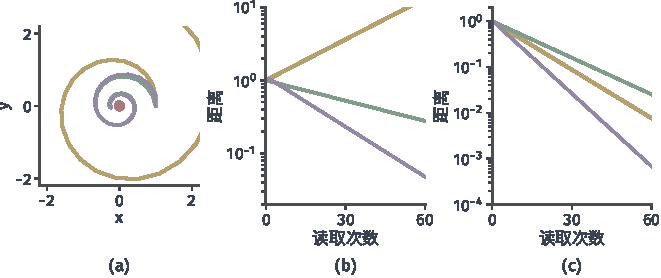
\includegraphics[width=112mm]{figures/05-optimization/07-multiple-criteria-and-nested-optimization/matplotlib/minimax-eg-paths/figure.pdf}
 \caption{三种方法的比较：黄线同时更新，绿线外梯度，紫线乐观梯度，起点$(1,0)$。(a)$f=xy$，$\alpha=0.3$，$30$轮的轨迹，红点是解。(b)$f=xy$到解的距离，横轴是方向读取次数，外梯度每轮计$2$次。(c)$f=\frac12x^2+2xy-\frac12y^2$，$\alpha=0.1$，同样按读取次数。}
 \label{fig:minimax-eg-paths}
\end{BookInlineFigure}

\subsection{乐观梯度法}
\label{sec:minimax-ogda}

\paragraph{主要思想}
外梯度法每轮读两次方向，能不能省一次？试探步的目的只是估计“下一步的方向”，而上一轮刚读过的方向已经是一个不错的估计。把试探步里的方向换成上一轮的$\bm{F}(\tilde{\bm{z}}^{(t-1)})$，无约束时得到
\[
 \tilde{\bm{z}}^{(t)}=\bm{z}^{(t)}-\alpha\bm{F}(\tilde{\bm{z}}^{(t-1)}),\qquad\bm{z}^{(t+1)}=\bm{z}^{(t)}-\alpha\bm{F}(\tilde{\bm{z}}^{(t)}).
\]
每轮只新读$\bm{F}(\tilde{\bm{z}}^{(t)})$一次。

把这个递推写成只含$\tilde{\bm{z}}$的形式。下一轮的试探点是
\[
 \tilde{\bm{z}}^{(t+1)}=\bm{z}^{(t+1)}-\alpha\bm{F}(\tilde{\bm{z}}^{(t)})=\bm{z}^{(t)}-2\alpha\bm{F}(\tilde{\bm{z}}^{(t)}).
\]
又由试探步，
\[
 \bm{z}^{(t)}=\tilde{\bm{z}}^{(t)}+\alpha\bm{F}(\tilde{\bm{z}}^{(t-1)}).
\]
代入后把$\tilde{\bm{z}}$重新记作$\bm{z}$，得到\term{乐观梯度下降—上升}（optimistic gradient descent--ascent，OGDA）：
\begin{equation}
 \bm{z}^{(t+1)}=\bm{z}^{(t)}-2\alpha\bm{F}(\bm{z}^{(t)})+\alpha\bm{F}(\bm{z}^{(t-1)}).
 \label{eq:minimax-ogda}
\end{equation}

把它写成
\[
 \bm{z}^{(t+1)}=\bm{z}^{(t)}-\alpha\bm{F}(\bm{z}^{(t)})-\alpha\bigl(\bm{F}(\bm{z}^{(t)})-\bm{F}(\bm{z}^{(t-1)})\bigr)
\]
就能看出它的含义。括号里是方向场在上一步中的变化量，代表耦合带来的转动。它按当前的变化趋势，把下一步的方向提前校正。“乐观”指相信方向场短期内的变化趋势会延续。它与重球动量的区别在于，重球叠加的是位置的差，这里叠加的是方向的差。

\paragraph{计算过程}
用$f=xy$，$\bm{F}(x,y)=(y,-x)$。

\needspace{6\baselineskip}
\paragraph{变量}
\begin{itemize}
 \item $\bm{z}^{(t)}$：当前点；
 \item $\bm{F}^{(t-1)}$：上一轮读到的方向，需要存储；
 \item $\alpha>0$：步长。
\end{itemize}

\paragraph{初始化}
取$\bm{z}^{(0)}$，并令$\bm{z}^{(-1)}=\bm{z}^{(0)}$，于是第一步就是普通的梯度步。例中$\bm{z}^{(0)}=(1,0)$，$\alpha=0.2$。

\needspace{6\baselineskip}
\paragraph{每轮更新}
\begin{enumerate}
 \item 读取当前方向$\bm{F}^{(t)}=\bm{F}(\bm{z}^{(t)})$。例中第一轮$\bm{F}^{(0)}=(0,-1)$，第二轮
 \[
  \bm{z}^{(1)}=(1,0.2),\qquad\bm{F}^{(1)}=(0.2,-1).
 \]
 \item 由式~\eqref{eq:minimax-ogda}更新，并保存$\bm{F}^{(t)}$。例中第二轮
 \[
  \bm{z}^{(2)}=(1,0.2)-0.4(0.2,-1)+0.2(0,-1)=(0.92,0.4).
 \]
\end{enumerate}

继续计算，得到
\[
 \bm{z}^{(3)}=(0.8,0.568),\qquad\bm{z}^{(4)}=(0.6528,0.704).
\]
距离的平方依次为$1,1.04,1.0064,0.9626,0.9218$，第一步因为没有历史而外漂，之后开始收缩。最终得到的迭代点沿螺旋线趋向鞍点，每轮只读一次方向。

\paragraph{双线性情形的稳定性}
线性的$\bm{F}$可以算到底。把$(x,y)$看作复数$w=x+\mathrm{i}y$，$\bm{F}=(y,-x)$对应$-\mathrm{i}w$，同时更新就成了$w^{+}=(1+\mathrm{i}\alpha)w$，与式~\eqref{eq:minimax-gda-growth}一致。式~\eqref{eq:minimax-ogda}成为二阶递推
\[
 w^{(t+1)}=(1+2\mathrm{i}\alpha)w^{(t)}-\mathrm{i}\alpha w^{(t-1)}.
\]
它的特征方程是$s^2-(1+2\mathrm{i}\alpha)s+\mathrm{i}\alpha=0$，判别式是
\[
 (1+2\mathrm{i}\alpha)^2-4\mathrm{i}\alpha=1-4\alpha^2.
\]

$0<\alpha\leq\frac12$时判别式非负，两根是$\frac12(1+2\mathrm{i}\alpha\pm\sqrt{1-4\alpha^2})$，模较大的那个满足
\begin{equation}
 \rho^2=\frac{1+\sqrt{1-4\alpha^2}}{2}<1.
 \label{eq:minimax-ogda-bilinear}
\end{equation}

$\alpha=0.2$时$\rho^2\approx0.958$，上面逐步算出的距离确实以这个比例下降。小步长时$\rho^2\approx1-\alpha^2$，和外梯度的式~\eqref{eq:minimax-eg-contraction}同阶。$\alpha>\frac12$时两根的虚部不同，由$\lvert s\rvert^2<1$可得稳定的条件是$\alpha<1/\sqrt{3}\approx0.577$，见图~\ref{fig:minimax-ogda-stability}(a)。外梯度的范围更宽，到$\alpha<1$。

\begin{BookInlineFigure}
 \centering
 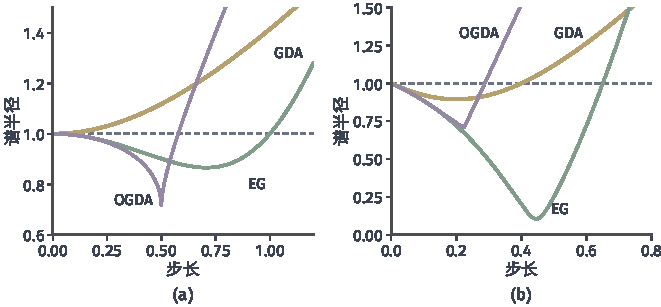
\includegraphics[width=112mm]{figures/05-optimization/07-multiple-criteria-and-nested-optimization/matplotlib/minimax-ogda-stability/figure.pdf}
 \caption{线性$\bm{F}$上的谱半径与步长的关系。虚线是稳定边界$1$。(a)$f=xy$：同时更新（GDA）全在边界之上。外梯度（EG）到$\alpha<1$稳定，乐观梯度（OGDA）到$\alpha<0.577$稳定。(b)$f=\frac12x^2+2xy-\frac12y^2$：三种方法都有稳定区间，分别到$0.4$、$0.65$、$0.29$。}
 \label{fig:minimax-ogda-stability}
\end{BookInlineFigure}

\paragraph{强凸—强凹情形}
取$f=\frac12x^2+2xy-\frac12y^2$，关于$x$强凸，关于$y$强凹，$\mu=1$。$\bm{F}$是线性的，其矩阵的特征值和Lipschitz常数是
\[
 \lambda=1\pm2\mathrm{i},\qquad L=\lvert\lambda\rvert=\sqrt5.
\]

同时更新和外梯度的每轮因子分别是$\lvert1-\alpha\lambda\rvert$和$\lvert1-\alpha\lambda+\alpha^2\lambda^2\rvert$。乐观梯度的因子是下面方程模较大的根：\[
 s^2-(1-2\alpha\lambda)s-\alpha\lambda=0.
\]

\begin{BookInlineTable}
 \centering
 \begin{tabular}{@{}llll@{}}
  \toprule
  方法 & $\alpha=0.1$ & $\alpha=0.2$ & 稳定上限\\
  \midrule
  GDA & $0.922$ & $0.894$ & $0.400$\\
  EG & $0.885$ & $0.721$ & $0.651$\\
  OGDA & $0.885$ & $0.739$ & $0.288$\\
  \bottomrule
 \end{tabular}
 \caption{$f=\frac12x^2+2xy-\frac12y^2$上三种方法的每轮收缩因子及步长上限（数值求得）。}
 \label{tab:minimax-sc-rates}
\end{BookInlineTable}

表~\ref{tab:minimax-sc-rates}的因子是按轮计算的，外梯度每轮读两次方向。按读取次数折算，$\alpha=0.1$时外梯度相当于每次读取收缩$\sqrt{0.885}\approx0.941$，比同时更新的$0.922$还慢，图~\ref{fig:minimax-eg-paths}(c)里绿线在黄线之上就是这个原因。外梯度的优势要靠较大的步长才能体现，图~\ref{fig:minimax-ogda-stability}(b)中它在$\alpha\approx0.45$处的每轮因子只有$0.105$。

对一般的强单调、Lipschitz算子，已知结论是外梯度和乐观梯度取$\alpha$为$1/L$量级时，每轮收缩因子是$1-O(\mu/L)$，而同时更新的步长要小到$\mu/L^2$量级，因子是$1-O(\mu^2/L^2)$。证明需要构造带历史项的势函数，篇幅较长，读者可查阅专门的变分不等式著作。

\paragraph{不能直接推广的情形}
上述核对都在单调问题上。$f=y^2-x^2$的$\bm{F}=(-2x,-2y)$，$\lambda=-2$，原点是排斥的：式~\eqref{eq:minimax-ogda}的特征方程$s^2-(1+4\alpha)s+2\alpha=0$在$s=1$处取值$-2\alpha<0$，所以有一根大于$1$。同样的计算也使外梯度的因子$1+2\alpha+4\alpha^2$大于$1$。

有约束时还要分清变体。把投影直接加到式~\eqref{eq:minimax-ogda}上，得到$P_{\bm{Z}}(\bm{z}^{(t)}-2\alpha\bm{F}(\bm{z}^{(t)})+\alpha\bm{F}(\bm{z}^{(t-1)}))$；另一种形式保留试探点和校正点两条序列，各做一次投影。无约束时二者等价，有约束时不是同一个递推。

例如在盒子$[-1,1]^2$上，$\bm{z}^{(0)}=(1,0.9)$，$\alpha=0.4$，$\bm{F}=(y,-x)$，第一步前者给出$(0.64,1)$，后者给出$(0.6,1)$。两种形式的步长条件和分析要分别核对，不能把其中一种的保证直接用到另一种，更不能推广到任意的非凸问题。

\section{结果评价}
\label{sec:minimax-evaluation}

算法停下来，交出一对$(\bm{x},\bm{y})$，它有多好？极小极大问题里，$f(\bm{x}^{(t)},\bm{y}^{(t)})$的升降不能回答这个问题，图~\ref{fig:minimax-gda-monitor}已经表明，两侧的优化方向本来相反，这个数上下波动没有确定的含义。

所以第一步是说清要评价什么。表~\ref{tab:minimax-evidence}按目标列出相应的证据。

\begin{BookInlineTable}
 \centering
 \begin{tabular}{@{}lll@{}}
  \toprule
  目标 & 证据 & 成立前提\\
  \midrule
  全局鞍点 & 间隙$G$或其有效上界 & 两侧极值能算或能界\\
  值函数最小 & $\phi$的（次）梯度 & 内层响应可信\\
  局部结构 & 二阶条件 & 只在邻域内有意义\\
  \bottomrule
 \end{tabular}
 \caption{评价目标与相应的证据。}
 \label{tab:minimax-evidence}
\end{BookInlineTable}

\subsection{误差证据}
\label{sec:minimax-error-evidence}

凸凹问题上最好的证据是间隙~\eqref{eq:minimax-gap}。若$\phi$和$\psi$能直接算出，例如$f$双线性而$\bm{X},\bm{Y}$是单纯形或盒子，内层就是线性函数在顶点上取值，这时间隙是精确的。

\paragraph{平均点与最后一点}
定理~\ref{thm:minimax-eg-gap}保证的是平均点。最后一点可能完全不同。在盒子$[-1,1]^2$上，$f=xy$，$L=1$，取外梯度法的边界步长$\alpha=1$，从$(1,0)$出发。第一轮试探点和校正点是
\[
 \tilde{\bm{z}}^{(0)}=(1,1),\qquad\bm{z}^{(1)}=(1,0)-(1,-1)=(0,1).
\]
继续下去，$\bm{z}^{(t)}$依次经过$(1,0),(0,1),(-1,0),(0,-1)$，每四轮回到起点。试探点依次是四个顶点。

由式~\eqref{eq:minimax-box-gap}，最后一点的间隙恒为$1$，没有收敛。而试探点的平均，$T=1,2,3,4$时间隙分别是$2,1,\frac23,0$，都不超过定理的上界$\frac{D^2}{2\alpha T}=\frac4T$，这里$D^2=8$，见图~\ref{fig:minimax-average-last}。

\begin{BookInlineFigure}
 \centering
 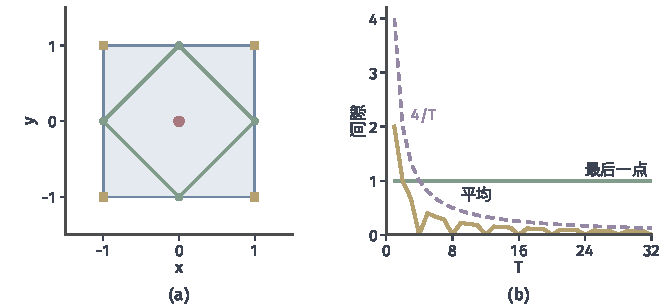
\includegraphics[width=112mm]{figures/05-optimization/07-multiple-criteria-and-nested-optimization/matplotlib/minimax-average-last/figure.pdf}
 \caption{外梯度法取边界步长$\alpha=1/L=1$，$f=xy$，$\bm{Z}=[-1,1]^2$，起点$(1,0)$。(a)绿点是校正点，沿菱形循环；黄色方块是试探点，在四个顶点循环；红点是鞍点。(b)绿线是最后一点的间隙，恒为$1$；黄线是试探点平均的间隙，在每四轮的整数倍处为$0$；紫色虚线是上界$4/T$。}
 \label{fig:minimax-average-last}
\end{BookInlineFigure}

$\alpha<1/L$时可以证明校正点本身收敛到某个鞍点，这个例子的循环出现在边界步长上。最后一点的间隙速率比平均点慢，一般是$O(1/\sqrt{T})$，证明较长，读者可查阅外梯度法最后迭代分析的专门文献。报告结果时要说清楚输出的是平均点还是最后一点，因为定理的结论只属于它所针对的那一个。

\paragraph{近似内层给出的间隙偏小}
$\phi$和$\psi$算不出来时，通常用内层算法分别求一个近似响应$\tilde{\bm{y}}$和近似外层点$\tilde{\bm{x}}$，然后计算
\begin{equation}
 \hat{G}=f(\bm{x},\tilde{\bm{y}})-f(\tilde{\bm{x}},\bm{y}).
 \label{eq:minimax-gap-estimate}
\end{equation}

因为$f(\bm{x},\tilde{\bm{y}})\leq\phi(\bm{x})$，$f(\tilde{\bm{x}},\bm{y})\geq\psi(\bm{y})$，所以$\hat{G}\leq G$。这与第~\ref{chap:duality}章“内层近似的方向”是同一个现象，误差方向正好不利：内层算得越粗糙，估计的间隙越小，算法看起来越好。

取盒子上的$f=xy$，候选$(x,y)=(0.4,-0.2)$，由式~\eqref{eq:minimax-box-gap}，真实间隙是$0.6$。内层只走一步步长$\frac12$的投影梯度：
\[
 \tilde{y}=-0.2+\frac12\cdot0.4=0,\qquad\tilde{x}=0.4-\frac12\cdot(-0.2)=0.5.
\]
式~\eqref{eq:minimax-gap-estimate}给出
\[
 \hat{G}=f(0.4,0)-f(0.5,-0.2)=0+0.1=0.1.
\]
真实间隙$0.6$被低估了六倍。

要得到可靠的上界，必须把内层误差补回去。第~\ref{chap:duality}章由梯度残差得到认证界：$\mu$强凸函数在$\tilde{\bm{x}}$处的最小值至少是函数值减去$\lVert\nabla\rVert_2^2/(2\mu)$。把它用到$-f(\bm{x},\cdot)$和$f(\cdot,\bm{y})$上。设$\bm{X}=\mathbb{R}^n$，$\bm{Y}=\mathbb{R}^q$，$f(\bm{x},\cdot)$是$\mu_y$强凹的，$f(\cdot,\bm{y})$是$\mu_x$强凸的，则
\begin{equation}
 G(\bm{x},\bm{y})\leq\hat{G}+\frac{\lVert\nabla_{\bm{y}}f(\bm{x},\tilde{\bm{y}})\rVert_2^2}{2\mu_y}+\frac{\lVert\nabla_{\bm{x}}f(\tilde{\bm{x}},\bm{y})\rVert_2^2}{2\mu_x}.
 \label{eq:minimax-certified-gap}
\end{equation}

验算一例。$f=\frac12x^2+2xy-\frac12y^2$，$\mu_x=\mu_y=1$，候选$(0.2,0.1)$。真实值由$\phi(x)=\frac52x^2$，$\psi(y)=-\frac52y^2$算出，
\[
 G=0.1+0.025=0.125.
\]

取近似响应$\tilde{y}=0.3$，$\tilde{x}=-0.1$，则
\[
 f(0.2,0.3)=0.095,\qquad f(-0.1,0.1)=-0.02,\qquad\hat{G}=0.115.
\]
两个残差是$\partial_yf(0.2,0.3)=0.1$，$\partial_xf(-0.1,0.1)=0.1$，式~\eqref{eq:minimax-certified-gap}的修正量各是$0.005$，得到上界
\[
 0.115+0.005+0.005=0.125.
\]
未修正的$\hat{G}$比真实间隙小，修正之后的上界不小于真实间隙。这里等号成立，因为函数恰好是二次的，曲率常数处处精确。

\subsection{非凸问题}
\label{sec:minimax-nonconvex}

没有凸凹性时，间隙可能恒为正，甚至恒为无穷，图~\ref{fig:minimax-saddle-types}(c)的原点就是这样。此时的目标是顺序问题本身，证据要分三层报告，各说明它证明了什么。

\paragraph{值函数的驻定证据}
内层强凹时，$\phi$可微，外层的驻定量可以由已知量给出上界。由三角不等式和式~\eqref{eq:minimax-gradient-error}，
\begin{equation}
 \lVert\nabla\phi(\bm{x})\rVert_2\leq\lVert\nabla_{\bm{x}}f(\bm{x},\tilde{\bm{y}})\rVert_2+L\sqrt{\frac{2\varepsilon}{\mu}}.
 \label{eq:minimax-stationarity-bound}
\end{equation}

用$f=-\frac12x^2+2xy-\frac12y^2$，取$x=0.1$，$\tilde{y}=0.18$。此时外层偏导数是$-0.1+0.36=0.26$，内层间隙是$\frac12(0.02)^2=0.0002$。交叉系数是$2$，第二项是$2\cdot0.02=0.04$，上界是$0.30$，真实导数$3x$也是$0.30$。

式~\eqref{eq:minimax-stationarity-bound}需要$\varepsilon$的可靠上界。内层强凹且无约束时，式~\eqref{eq:minimax-certified-gap}用到的残差界同样适用，$\varepsilon$不超过残差平方除以$2\mu$；有约束时要用相应的对偶界。

\paragraph{响应求解的证据}
内层不凹时，$\varepsilon$一般没有可计算的上界。从多个起点运行内层算法，取最大的值作为$\phi(\bm{x})$的估计，这是一个越算越大的下界。报告时要写成“在所检查的响应中最坏值是多少”，并说明检查的范围。它不是全局最坏值。式~\eqref{eq:minimax-nonconcave}在$x=1$处，从$y<-0.618$出发只能得到$0.25$，从$y>-0.618$出发才能得到$3.023$。

\paragraph{局部极小极大条件}
不要求全局最坏时，可以问一个更弱的问题：相对于局部的响应分支，当前点是不是极小？下面的二阶充分条件给出一种准确的说法。

\begin{theorem}[局部极小极大的二阶充分条件]
\label{thm:minimax-local}
设$f$在$(\bar{\bm{x}},\bar{\bm{y}})$附近二阶连续可微，$\nabla_{\bm{x}}f$和$\nabla_{\bm{y}}f$在该点为零，$\nabla^2_{\bm{y}\bm{y}}f\prec\bm{0}$，并且
\begin{equation}
 \bm{S}=\nabla^2_{\bm{x}\bm{x}}f-\nabla^2_{\bm{x}\bm{y}}f\,(\nabla^2_{\bm{y}\bm{y}}f)^{-1}\,\nabla^2_{\bm{y}\bm{x}}f\succ\bm{0}.
 \label{eq:minimax-schur}
\end{equation}
则存在定义在$\bar{\bm{x}}$某邻域上的连续可微映射$\bm{y}(\bm{x})$，$\bm{y}(\bar{\bm{x}})=\bar{\bm{y}}$，使$\bm{y}(\bm{x})$是$f(\bm{x},\cdot)$的局部极大点，且$\bar{\bm{x}}$是$\bm{x}\mapsto f(\bm{x},\bm{y}(\bm{x}))$的严格局部极小点。称这样的$(\bar{\bm{x}},\bar{\bm{y}})$为\term{局部极小极大点}（local minimax point）。
\end{theorem}

\begin{proof}
方程$\nabla_{\bm{y}}f(\bm{x},\bm{y})=\bm{0}$在该点关于$\bm{y}$的Jacobian是$\nabla^2_{\bm{y}\bm{y}}f$，可逆。隐函数定理给出连续可微的$\bm{y}(\bm{x})$，其导数是
\[
 \nabla\bm{y}(\bm{x})=-(\nabla^2_{\bm{y}\bm{y}}f)^{-1}\nabla^2_{\bm{y}\bm{x}}f.
\]
由连续性，$\nabla^2_{\bm{y}\bm{y}}f$在邻域内保持负定，所以$\bm{y}(\bm{x})$是局部极大点。

令$h(\bm{x})=f(\bm{x},\bm{y}(\bm{x}))$。因为在响应分支上$\nabla_{\bm{y}}f=\bm{0}$，链式法则只留下关于$\bm{x}$的偏梯度：
\[
 \nabla h(\bm{x})=\nabla_{\bm{x}}f(\bm{x},\bm{y}(\bm{x})).
\]
再求一次导，得到
\[
 \nabla^2h=\nabla^2_{\bm{x}\bm{x}}f+\nabla^2_{\bm{x}\bm{y}}f\,\nabla\bm{y}(\bm{x}).
\]
代入$\nabla\bm{y}$的表达式，在$\bar{\bm{x}}$处就是$\bm{S}$。又$\nabla h(\bar{\bm{x}})=\bm{0}$，$\bm{S}\succ\bm{0}$，由二阶充分条件，$\bar{\bm{x}}$是$h$的严格局部极小点。
\end{proof}

对$f=-\frac12x^2+2xy-\frac12y^2$，$\nabla^2_{yy}f=-1$，$S=-1-2\cdot(-1)\cdot2=3$，恰好是$\phi''$。

这个条件只回答局部响应分支。把式~\eqref{eq:minimax-nonconcave}放到$(1,-1)$处，两个偏导数$x+y$和$x+2y-y^3$都是$0$，$\partial_y^2f=2-3y^2=-1<0$，$\partial_x^2f=1$，$\partial_{xy}f=1$，
\[
 S=1-1\cdot(-1)\cdot1=2>0.
\]
定理的全部条件都满足，$(1,-1)$是局部极小极大点。可是$\phi'(1)=2.618\neq0$，$\phi(1)=3.023$，而外层真正的最优解是$x=0$。局部极小极大是相对于“内层只能看到附近”这个模型的结论，不能当作原问题的解来报告。

\paragraph{计算预算}
不同方法每轮的工作量相差悬殊，一轮精确内解和一轮下降—上升不能直接比较。图~\ref{fig:minimax-budget}是同一组运行的两种画法。(a)按外层轮数，$K=1$明显落后，$K=10$几乎与精确响应重合，$K=3$在这组系数下收缩最快；(b)按梯度读取总数，$K=10$反而最慢，因为它每轮要读$11$次。

\begin{BookInlineFigure}
 \centering
 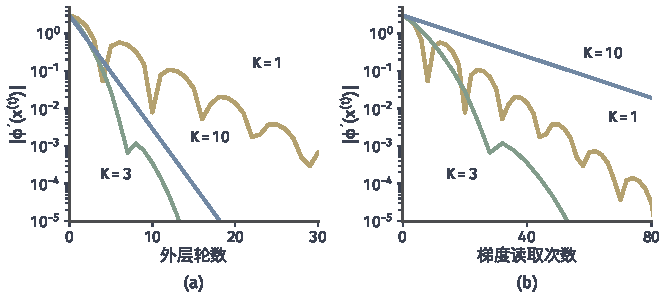
\includegraphics[width=112mm]{figures/05-optimization/07-multiple-criteria-and-nested-optimization/matplotlib/minimax-budget/figure.pdf}
 \caption{$f=-\frac12x^2+2xy-\frac12y^2$上每轮做$K$步内层上升的方法，$\alpha=\frac16$，$\beta=\frac12$，起点$(1,0)$。黄线$K=1$，绿线$K=3$，蓝线$K=10$。(a)按外层轮数，灰色虚线是精确响应。(b)同样的运行按梯度读取次数，每轮读取$K+1$次。}
 \label{fig:minimax-budget}
\end{BookInlineFigure}

报告的预算应当分开写明外层迭代次数、每次内层的计算量以及方向读取的总次数。这个例子里内层便宜且条件好，$K=3$在读取次数上最省。换一个问题，这个顺序可以完全不同。

\section{本章小结}
\label{sec:minimax-summary}

本章研究固定代价$f$下的问题$\inf_{\bm{x}}\sup_{\bm{y}}f$，它有两层结构：外层最小化，内层取最坏情形。开头的三个困难，分别由最坏值函数、鞍点和更新动力学来回答，这三者回答的是不同的问题。

\begin{BookInlineTable}
 \centering
 \begin{tabular}{@{}lll@{}}
  \toprule
  工具 & 回答的问题 & 依赖的条件\\
  \midrule
  最坏值函数$\phi$ & 外层在最小化什么 & $\bm{Y}$紧时连续，响应唯一时可微\\
  全局鞍点与间隙 & 一对候选是否全局解 & 紧凸且凸凹时存在\\
  迭代动力学 & 算法会不会靠近解 & 单调性、Lipschitz性、步长\\
  \bottomrule
 \end{tabular}
 \caption{本章的三个主要工具。}
 \label{tab:minimax-summary}
\end{BookInlineTable}

顺序极小极大问题与同时下降—上升算法是两回事。前者是要解的数学问题，后者是一种迭代格式。图~\ref{fig:minimax-saddle-types}(c)的原点是顺序问题的解，却不是鞍点；$f=xy$上的同时更新发散，问题本身却有鞍点。

判断一个结果可信，要分别核对四项条件：
\begin{enumerate}
 \item 最值交换。只有凸凹性和相应的紧性成立时才能交换$\inf$和$\sup$，值相等还要另外核对达到，才有鞍点。
 \item 内层准确性。Danskin公式要全局最优响应，局部极大不能代替。强凹时内层间隙能转成外层梯度的误差，非凹时梯度残差小不保证接近最坏值。
 \item 耦合迭代的稳定。反对称的耦合产生旋转，下降—上升在双线性问题上不收敛。内层强凹时要让$\bm{y}$跟得上，单调问题上可以用外梯度或乐观梯度校正方向。
 \item 最终误差。间隙是全局证书，但只用近似内层算出的间隙偏小，需要修正；限定间隙和局部二阶条件都不能冒充全局结论。
\end{enumerate}

本章两层共用同一个代价$f$，内层想让$f$大，外层想让$f$小。下一章的两层目标各不相同，外层依赖内层的最优解，那时值函数的导数不再由这样简单的公式给出。


\chapter{双层优化}
\label{chap:bilevel-optimization}

用一个数$x\geq0$控制一次拟合的保守程度：$x$越大，拟合结果越被压向零。对每个$x$，先解一个拟合问题，得到结果$y$；再拿$y$和另一个固定的数比较，判断$x$选得好不好。要评价一个$x$，必须先完成一次优化。这样的问题里，决策分成两层，上面一层的目标要读取下面一层的最优解。

这种嵌套带来三个问题。第一，下面一层可能无解，也可能有许多个同样好的解，“把内解代入外层”这句话要先说清选的是哪一个。第二，外层要下降就要知道目标对$x$的导数，而内解没有显式公式。第三，所有计算都只是近似，内层没解准、线性方程没解准、外层没走完，这几种误差要分开核算。

本章依次回答这三个问题。第~\ref{sec:bilevel-problem}节确定数学对象，区分唯一内解、多解选择和有限步输出。第~\ref{sec:bilevel-solution-map}节检查内解能否沿一条分支光滑变化，以及分支在什么地方断开。第~\ref{sec:bilevel-implicit}节和第~\ref{sec:bilevel-unrolling}节给出两种求导路线，前者只看解点处的方程，后者沿算法的每一步传播导数。第~\ref{sec:bilevel-single-level}节换一种思路，把内层最优性写成约束。第~\ref{sec:bilevel-outer}节把三类误差放在一起，给出外层的求解和停止依据。

\section{双层问题}
\label{sec:bilevel-problem}

外层目标依赖内层的最优解时，它到底是一个什么样的函数？先把两层的角色写下来。

外层变量记为$\bm{x}\in\bm{C}\subseteq\mathbb{R}^n$，内层变量记为$\bm{y}\in\mathbb{R}^d$。外层选定$\bm{x}$之后，内层在可行集$\bm{Y}(\bm{x})\subseteq\mathbb{R}^d$上最小化自己的目标$g$；外层再用另一个目标$F$评价内层的结果。

\begin{definition}[内层解集]
\label{def:bilevel-inner-solutions}
给定$\bm{x}\in\bm{C}$，称
\begin{equation}
 \bm{S}(\bm{x})=\argmin_{\bm{y}\in\bm{Y}(\bm{x})}g(\bm{x},\bm{y})
 \label{eq:bilevel-solution-set}
\end{equation}
为\term{内层解集}（lower-level solution set），其中的点称为内解。外层目标$F(\bm{x},\bm{y})$只对内解作评价，由此形成的嵌套问题称为\term{双层优化}（bilevel optimization）问题。
\end{definition}

图~\ref{fig:bilevel-structure}是这个结构的全貌。$\bm{x}$有两条路影响外层：一条直接进入$F$，另一条先改变内层问题，再通过选出的内解起作用。外层只能修改$\bm{x}$，不能直接修改$\bm{y}$。中间的“选解规则”一格是定义里没有出现、却必不可少的一步，第~\ref{sec:bilevel-selection}小节会讲它。

\begin{BookInlineFigure}
 \centering
 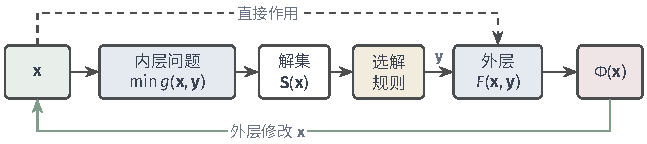
\includegraphics[width=109.6mm]{figures/05-optimization/07-multiple-criteria-and-nested-optimization/tikz/bilevel-structure/figure.pdf}
 \caption{双层问题的结构。外层变量$\bm{x}$决定内层问题，内层解集经选解规则给出$\bm{y}$，外层目标$F$再读取$\bm{y}$得到$\Phi(\bm{x})$。虚线是$\bm{x}$对$F$的直接作用，绿线表示外层根据$\Phi$修改$\bm{x}$。}
 \label{fig:bilevel-structure}
\end{BookInlineFigure}

\paragraph{内层无解时外层没有输入}
解集可能是空集。取外层变量$x\in\mathbb{R}$，内层变量$y\in\mathbb{R}$，内层目标是
\[
 g(x,y)=\frac{x}{2}y^2-y.
\]

$x>0$时这是开口向上的抛物线，唯一的内解是$y=1/x$。$x=0$时$g=-y$，$x<0$时$g$是开口向下的抛物线，两种情况下$y\to+\infty$都使$g\to-\infty$，内层没有最小点。

这时一个内层算法仍然可以运行并输出数字。比如梯度下降的更新是$y\leftarrow y+\alpha(1-xy)$，在$x<0$时迭代会不断增大。把这种数字交给外层，得到的外层值不评价任何内解。因此外层只在下面的集合上比较：
\begin{equation}
 \operatorname{dom}\bm{S}=\{\bm{x}\in\bm{C}:\bm{S}(\bm{x})\neq\varnothing\}.
 \label{eq:bilevel-dom}
\end{equation}
集合之外的$\bm{x}$一律视为外层不可行，外层值规定为$+\infty$。

\paragraph{与极小极大的区别}
第~\ref{chap:minimax-optimization}章的问题$\min_{\bm{x}}\max_{\bm{y}}f(\bm{x},\bm{y})$也是嵌套的，形式上取$g=-f$、$F=f$就是双层问题。可是那里两层围绕同一个代价相反地优化，内层的最优性恰好让外层目标对$\bm{y}$的偏导为零。双层问题的两个目标一般无关，内层最优并不让$F$在$\bm{y}$方向驻定，内解移动一点，外层值就跟着变化。表~\ref{tab:bilevel-vs-minimax}对比两者，第~\ref{sec:bilevel-hypergradient}小节会用公式说明最后一行。

\begin{BookInlineTable}
 \centering
 \begin{tabular}{lll}
  \toprule
  & 极小极大 & 双层优化\\
  \midrule
  内外目标 & 同一个$f$，方向相反 & $g$与$F$一般无关\\
  内解处$\nabla_{\bm{y}}F$ & 为零 & 一般不为零\\
  外层导数 & 无需内解的响应项 & 必须计入内解的响应\\
  \bottomrule
 \end{tabular}
 \caption{极小极大与双层优化的对比。第二、三行假定内解唯一、位于内层可行集内部且相关函数可微。}
 \label{tab:bilevel-vs-minimax}
\end{BookInlineTable}

\subsection{唯一内解}
\label{sec:bilevel-unique}

最简单的情形是对每个$\bm{x}$，解集恰有一个点，$\bm{S}(\bm{x})=\{\bm{y}^\star(\bm{x})\}$。这时选解不成问题，外层目标是一个普通的函数。

\begin{definition}[外层目标]
\label{def:bilevel-outer}
设对每个$\bm{x}\in\bm{C}$内解唯一，记为$\bm{y}^\star(\bm{x})$。外层问题是在$\bm{C}$上最小化
\begin{equation}
 \Phi(\bm{x})=F(\bm{x},\bm{y}^\star(\bm{x})).
 \label{eq:bilevel-phi}
\end{equation}
\end{definition}

$\Phi$的变化有两个来源。$\bm{x}$变动时，$F$的第一个位置直接变，这是直接作用；$\bm{y}^\star(\bm{x})$随之移动，$F$的第二个位置也变，这是响应。后者才是双层问题的特点，第~\ref{sec:bilevel-implicit}节专门计算它。

\paragraph{贯穿全章的正则拟合例}
下面的例子贯穿全章。内层用观测值$3$拟合一个数$y$，并用$x\geq0$惩罚$y$的大小；外层把结果和另一个固定的数$1$比较：
\begin{equation}
 g(x,y)=\frac12(y-3)^2+\frac{x}{2}y^2,\qquad F(x,y)=\frac12(y-1)^2.
 \label{eq:bilevel-ridge}
\end{equation}

对$y$求导并令导数为零，得到$(1+x)y-3=0$。$x\geq0$时$g$对$y$的二阶导数是$1+x>0$，所以内解唯一：
\begin{equation}
 y^\star(x)=\frac{3}{1+x}.
 \label{eq:bilevel-ridge-solution}
\end{equation}

代入式~\eqref{eq:bilevel-phi}，外层目标是
\[
 \Phi(x)=\frac12\Bigl(\frac{3}{1+x}-1\Bigr)^2.
\]
当$x=2$时内解恰好等于$1$，$\Phi$取到最小值$0$。

\paragraph{两个目标为什么不能合并}
看图~\ref{fig:bilevel-reaction}(a)。粗线是$y^\star(x)$的图像，只有粗线上的点才算内层最优。若把$x$和$y$一起放进$g$里最小化，得到的是空心点$(0,3)$，因为惩罚对$g$只是一种代价，$g$总愿意取$x=0$。若把两者一起放进$F$里最小化，虚线$y=1$上每一点都是最优的，$x$完全不起作用，等于直接把拟合结果改成想要的数。

双层结构要求的是第三种做法：沿粗线走，在粗线上找$F$最小的点。这正像预算线上的最优：可选的点被限制在一条曲线上，只不过这条曲线本身要靠解优化问题才能画出来。图~\ref{fig:bilevel-reaction}(b)把粗线上的外层值画成$x$的函数，最小点在$x=2$。

\begin{BookInlineFigure}
 \centering
 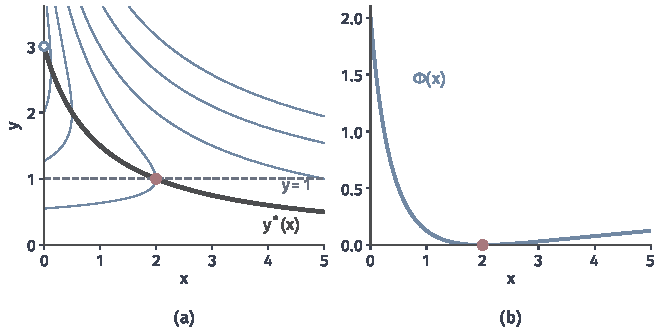
\includegraphics[width=112mm]{figures/05-optimization/07-multiple-criteria-and-nested-optimization/matplotlib/bilevel-reaction/figure.pdf}
 \caption{正则拟合例~\eqref{eq:bilevel-ridge}。(a)蓝色细线是内层目标$g$的等高线，空心点$(0,3)$是$g$对$(x,y)$的最小点；深灰粗线是内解曲线$y^\star(x)=3/(1+x)$；虚线$y=1$上$F$取最小值；红点$(2,1)$是双层问题的解。(b)外层目标$\Phi(x)$，最小点是$x=2$。}
 \label{fig:bilevel-reaction}
\end{BookInlineFigure}

\paragraph{直接作用的例子}
式~\eqref{eq:bilevel-ridge}中$F$不含$x$，全部变化都来自响应。若外层再为$x$付出代价，比如把$F$换成$\frac12(y-1)^2+\frac{1}{10}x$，直接作用就出现了：$\Phi$多了一项$\frac{1}{10}x$，最小点从$x=2$向左移动。两个来源在导数中分别对应一项。

这里的$3$和$1$只是两个固定的数，本章把它们当作给定的优化数据。数据该怎样划分，这样选出的$x$有没有统计上的保证，不是优化问题，可参考\BookChapterRef{chap:finite-sample-error-bounds}{卷八第4章“有限样本的误差上界”}。

\subsection{多解选择}
\label{sec:bilevel-selection}

解集可能含有许多点，它们对内层来说一样好，对外层却可能差别很大。这时$F(\bm{x},\bm{y}^\star(\bm{x}))$这个写法失去了意义，必须补充一条规则。

\paragraph{两种选解规则}
可以用一个比喻来理解。外层是提要求的一方，内层是执行的一方，执行方在几个同样好的方案之间不在乎选哪个。外层可以假定执行方会配合自己，也可以防备它选最不利的。这个比喻只用来记住两种规则，数学上并不要求内层真有什么意愿，规则只是对解集中的点作出约定。

\begin{definition}[乐观模型与悲观模型]
\label{def:bilevel-opt-pes}
对$\bm{x}\in\operatorname{dom}\bm{S}$，定义
\begin{align}
 \Phi_{\mathrm{o}}(\bm{x})&=\inf_{\bm{y}\in\bm{S}(\bm{x})}F(\bm{x},\bm{y}),
 \label{eq:bilevel-optimistic}\\
 \Phi_{\mathrm{p}}(\bm{x})&=\sup_{\bm{y}\in\bm{S}(\bm{x})}F(\bm{x},\bm{y}),
 \label{eq:bilevel-pessimistic}
\end{align}
对$\bm{x}\notin\operatorname{dom}\bm{S}$，两者都规定为$+\infty$。在$\bm{C}$上最小化$\Phi_{\mathrm{o}}$称为\term{乐观模型}（optimistic model），最小化$\Phi_{\mathrm{p}}$称为\term{悲观模型}（pessimistic model）。
\end{definition}

空集上的规定要单独写出。按惯例$\sup\varnothing=-\infty$，若照搬，内层无解的$\bm{x}$在悲观模型中外层值是$-\infty$，反而成了最好的选择，这与第~\ref{sec:bilevel-problem}节开头的约定相反。

两个函数处处满足$\Phi_{\mathrm{o}}\leq\Phi_{\mathrm{p}}$，内解唯一时都等于$\Phi$。乐观模型的$\inf$可以和外层的$\inf$合并，于是
\begin{equation}
 \inf_{\bm{x}\in\bm{C}}\Phi_{\mathrm{o}}(\bm{x})=\inf\{F(\bm{x},\bm{y}):\bm{x}\in\bm{C},\ \bm{y}\in\bm{S}(\bm{x})\}.
 \label{eq:bilevel-optimistic-joint}
\end{equation}
乐观模型因而是一个对$(\bm{x},\bm{y})$的联合最小化，可行集是解集的图像。悲观模型夹着一层$\sup$，不能这样合并。

\paragraph{一个手算例子}
取$\bm{C}$和内层可行集都是$[-1,1]$，目标是
\[
 g(x,y)=xy,\qquad F(x,y)=x^2+y.
\]

内层在$[-1,1]$上最小化关于$y$的线性函数，解由$x$的符号决定：
\[
 S(x)=\begin{cases}
 \{1\}, & x<0,\\
 [-1,1], & x=0,\\
 \{-1\}, & x>0.
 \end{cases}
\]

$x\neq0$时只有一个内解，两种模型相同：$x<0$时外层值是$x^2+1$，$x>0$时外层值是$x^2-1$。分歧只在$x=0$，此时整个区间都是内解，$F(0,y)=y$，于是
\[
 \Phi_{\mathrm{o}}(0)=-1,\qquad\Phi_{\mathrm{p}}(0)=1.
\]

图~\ref{fig:bilevel-selection}画出了这个例子。乐观模型在$x=0$取到最小值$-1$，红点就是它的解。悲观模型的下确界同样是$-1$，因为$x\downarrow0$时$x^2-1\to-1$，但这个值取不到：$x=0$处值跳到$1$，$x>0$时值严格大于$-1$。悲观模型没有最优解。

\begin{BookInlineFigure}
 \centering
 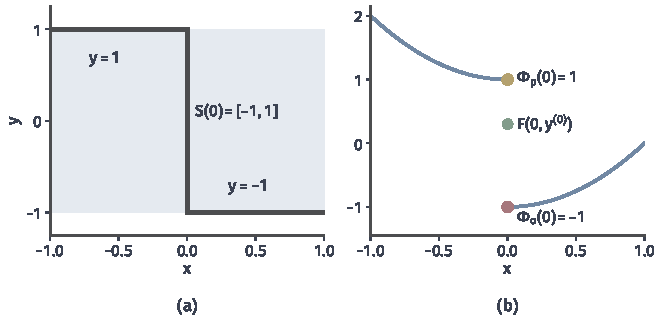
\includegraphics[width=112mm]{figures/05-optimization/07-multiple-criteria-and-nested-optimization/matplotlib/bilevel-selection/figure.pdf}
 \caption{多解时的选解。内层$g=xy$，$x,y\in[-1,1]$，外层$F=x^2+y$。(a)浅蓝是内层可行集，深灰线是解集$S(x)$的图像，$x=0$处是整段区间。(b)蓝线是$x\neq0$时共同的外层值。$x=0$处，红点是乐观值，黄点是悲观值，绿点是从$y^{(0)}=0.3$出发的投影梯度法实际得到的外层值。}
 \label{fig:bilevel-selection}
\end{BookInlineFigure}

\paragraph{乐观模型的解存在，悲观模型没有这样的保证}
上例不是偶然的。把式~\eqref{eq:bilevel-optimistic-joint}看成解集图像上的最小化，就可以套用第~\ref{chap:optimization}章的存在定理，只需说明图像是紧的。

\begin{theorem}[乐观模型解的存在]
\label{thm:bilevel-optimistic-existence}
设$\bm{C}$和$\bm{Y}$是非空紧集，内层可行集恒为$\bm{Y}$，$g$和$F$在$\bm{C}\times\bm{Y}$上连续。则集合
\begin{equation}
 \bm{G}=\{(\bm{x},\bm{y}):\bm{x}\in\bm{C},\ \bm{y}\in\bm{S}(\bm{x})\}
 \label{eq:bilevel-graph}
\end{equation}
非空且紧，乐观模型有最优解。
\end{theorem}

\begin{proof}
对每个$\bm{x}\in\bm{C}$，连续函数$g(\bm{x},\cdot)$在紧集$\bm{Y}$上取得最小值，所以$\bm{S}(\bm{x})$非空，$\bm{G}$非空。$\bm{G}$含于紧集$\bm{C}\times\bm{Y}$，只需证明它是闭集。

取$\bm{G}$中收敛到$(\bm{x},\bm{y})$的序列$(\bm{x}^{(k)},\bm{y}^{(k)})$。$\bm{C}$、$\bm{Y}$闭，所以$\bm{x}\in\bm{C}$，$\bm{y}\in\bm{Y}$。任取比较点$\bm{z}\in\bm{Y}$，由$\bm{y}^{(k)}$是内解，有
\[
 g(\bm{x}^{(k)},\bm{y}^{(k)})\leq g(\bm{x}^{(k)},\bm{z}).
\]

令$k\to\infty$，由$g$连续，得到
\[
 g(\bm{x},\bm{y})\leq g(\bm{x},\bm{z}).
\]
$\bm{z}$是任取的，所以$\bm{y}\in\bm{S}(\bm{x})$，$\bm{G}$是闭集。连续函数$F$在紧集$\bm{G}$上取得最小值，由式~\eqref{eq:bilevel-optimistic-joint}，它就是乐观模型的最优值。
\end{proof}

前面的例子满足定理的全部条件，悲观模型却没有解。原因是第~\ref{chap:optimization}章存在论证的第三关：悲观目标在$x=0$处向上跳，不是下半连续的。

\paragraph{算法的隐含择解}
实际运行时，算法既不会自动做$\inf$，也不会自动做$\sup$。上例中$x=0$时内层梯度是$\partial_yg=x=0$，投影梯度法根本不动，停在初值。从$y^{(0)}=0.3$出发，得到外层值$F(0,0.3)=0.3$，这就是图~\ref{fig:bilevel-selection}(b)的绿点，它既不是乐观值，也不是悲观值。

所以声称求解某个模型时，要说清算法的输出怎样对应这个模型；对应不上的话，算出来的只是“这个算法从这个初值给出的外层值”。

\subsection{有限步内解}
\label{sec:bilevel-finite}

精确内解通常拿不到，实际手里的是算法运行若干步的结果。这个结果也是$\bm{x}$的函数，但它和内解是不同的对象。

\begin{definition}[有限步目标]
\label{def:bilevel-finite}
给定内层算法的初始化和更新规则，把运行$T$步的输出记为$\bm{y}^{(T)}(\bm{x})$。称
\begin{equation}
 \Phi_T(\bm{x})=F(\bm{x},\bm{y}^{(T)}(\bm{x}))
 \label{eq:bilevel-finite-objective}
\end{equation}
为\term{有限步目标}（finite-step objective）。
\end{definition}

这个函数依赖初值、更新规则、步长和步数，换掉任何一项就是另一个函数。

\paragraph{用正则拟合例计算}
对式~\eqref{eq:bilevel-ridge}的内层用梯度下降，初值$y^{(0)}=0$，步长$\alpha=1/2$。内层梯度是$(1+x)y-3$，代入更新式，得到
\[
 y^{(t+1)}=y^{(t)}-\frac12\bigl[(1+x)y^{(t)}-3\bigr]=q\,y^{(t)}+\frac32,\qquad q=\frac{1-x}{2}.
\]

减去不动点$y^\star(x)$，误差每步乘$q$，初始误差是$-y^\star(x)$，所以
\begin{equation}
 y^{(T)}(x)=y^\star(x)\bigl(1-q^T\bigr).
 \label{eq:bilevel-ridge-finite}
\end{equation}

$T$较小时可以写成多项式。前两步的结果是
\[
 y^{(1)}=\frac32,\qquad y^{(2)}=\frac94-\frac34x.
\]

$y^{(1)}$与$x$无关，于是$\Phi_1$是常数，走一步完全看不到$x$的作用。$\Phi_2$的最小点由$y^{(2)}=1$确定，得到$x=5/3$，与$\Phi$的最小点$x=2$不同。

再看$T=3$。直接计算得$y^{(3)}=\frac32(q^2+q+1)$，它在$q=-1/2$时最小，最小值是$9/8$。这时$y^{(3)}$到不了$1$，$\Phi_3$的最小点是$x=2$，最小值却是$1/128$，不是$0$。图~\ref{fig:bilevel-finite-step}比较了几个$T$。

\begin{BookInlineFigure}
 \centering
 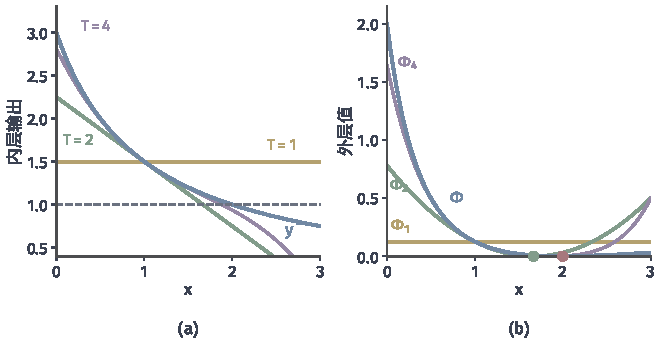
\includegraphics[width=112mm]{figures/05-optimization/07-multiple-criteria-and-nested-optimization/matplotlib/bilevel-finite-step/figure.pdf}
 \caption{有限步内解与有限步目标，内层梯度下降取$y^{(0)}=0$、$\alpha=1/2$。(a)内层输出$y^{(T)}(x)$（$T=1,2,4$）与精确内解$y^\star(x)$（蓝）；所有曲线在$x=1$相交，因为此时$q=0$，一步即得精确解。(b)对应的$\Phi_T$与$\Phi$。绿点是$\Phi_2$的最小点$x=5/3$，红点是$\Phi$的最小点$x=2$。}
 \label{fig:bilevel-finite-step}
\end{BookInlineFigure}

\paragraph{设计目标还是近似手段}
这里要区分两种立场。第一种，最终交付的就是“运行$T$步的这个过程”，$T$和初值是设计的一部分，那么$\Phi_T$本身就是要优化的目标，它的梯度是精确的，不必谈$\bm{y}^\star$。第二种，真正关心的是最优选解，$T$步只是不得已的近似，那么$\Phi_T$与$\Phi$的差别就是要核算的误差。

两种立场下同一个数字含义不同，不能因为运行的是优化算法，就把$\bm{y}^{(T)}(\bm{x})$称作$\bm{y}^\star(\bm{x})$。表~\ref{tab:bilevel-objects}列出本节得到的三个对象。

\begin{BookInlineTable}
 \centering
 \begin{tabular}{lll}
  \toprule
  对象 & 需要说明什么 & 依赖\\
  \midrule
  内解唯一的$\Phi$ & 唯一性 & 问题本身\\
  $\Phi_{\mathrm{o}}$、$\Phi_{\mathrm{p}}$ & 乐观或悲观 & 问题与规则\\
  $\Phi_T$ & 初值、更新、步数 & 算法实现\\
  \bottomrule
 \end{tabular}
 \caption{外层目标的三种对象。内层无解的$\bm{x}$不属于前两行的讨论范围。}
 \label{tab:bilevel-objects}
\end{BookInlineTable}

\section{内层解映射}
\label{sec:bilevel-solution-map}

外层要下降，需要知道$\Phi$的导数，而$\Phi$里含着内解。内解能不能看成$\bm{x}$的光滑函数？这个问题要分范围回答，因为“内解”可以指三种不同范围的东西：全局解集、某个局部极小点所在的分支，以及只满足驻点方程的点。

第~\ref{chap:parametric-sensitivity}章已经研究过解随参数的变化。本节把那里的结论放到双层语境中使用：先确定追踪的是哪个范围的分支，再讨论能否对它求导。

\subsection{可微分支}
\label{sec:bilevel-branch}

先看无约束内层，$\bm{Y}(\bm{x})=\mathbb{R}^d$。内层的碗底满足驻点方程$\nabla_{\bm{y}}g=\bm{0}$。外层变量一动，碗的形状变化，碗底跟着移动，移动多少由碗的曲率决定：曲率大的方向，碗底只需挪一点就能抵消梯度的变化。

\paragraph{局部分支}
记$(\bm{x}_0,\bm{y}_0)$为基准点。下面的定理就是第~\ref{chap:parametric-sensitivity}章的无约束解导数定理，这里按双层记号复述。

\begin{theorem}[局部极小分支]
\label{thm:bilevel-local-branch}
设$g$在$(\bm{x}_0,\bm{y}_0)$的邻域内二阶连续可微，$\nabla_{\bm{y}}g(\bm{x}_0,\bm{y}_0)=\bm{0}$，且$\nabla^2_{\bm{y}\bm{y}}g(\bm{x}_0,\bm{y}_0)\succ\bm{0}$。则存在$\bm{x}_0$的邻域$\bm{U}$、$\bm{y}_0$的邻域$\bm{V}$和唯一的连续可微映射$\hat{\bm{y}}:\bm{U}\to\bm{V}$，使$\hat{\bm{y}}(\bm{x}_0)=\bm{y}_0$，并且对$\bm{x}\in\bm{U}$有
\begin{equation}
 \nabla_{\bm{y}}g(\bm{x},\hat{\bm{y}}(\bm{x}))=\bm{0},
 \label{eq:bilevel-branch-stationary}
\end{equation}
每个$\hat{\bm{y}}(\bm{x})$都是$g(\bm{x},\cdot)$的严格局部极小点。其Jacobian矩阵为
\begin{equation}
 \bm{D}(\bm{x})=\frac{\partial\hat{\bm{y}}}{\partial\bm{x}}=-\bm{H}^{-1}\bm{B},
 \label{eq:bilevel-branch-derivative}
\end{equation}
其中$\bm{H}=\nabla^2_{\bm{y}\bm{y}}g$是$d\times d$矩阵，$\bm{B}=\nabla^2_{\bm{y}\bm{x}}g$是$d\times n$矩阵，其$(i,j)$元素是$\partial^2g/\partial y_i\partial x_j$，两者都在$(\bm{x},\hat{\bm{y}}(\bm{x}))$处取值。
\end{theorem}

\begin{proof}
把驻点方程$\nabla_{\bm{y}}g(\bm{x},\bm{y})=\bm{0}$看成$d$个方程、$d$个未知量$\bm{y}$、参数$\bm{x}$的系统。它对$\bm{y}$的Jacobian矩阵是$\bm{H}$，在基准点正定，因而可逆。隐函数定理给出邻域和唯一的连续可微分支，定理的陈述可参考\BookChapterRef{chap:implicit-inverse-functions}{卷二第22章“隐函数与反函数”}。

沿分支式~\eqref{eq:bilevel-branch-stationary}恒成立，对$\bm{x}$求导，得到
\[
 \bm{H}\bm{D}+\bm{B}=\bm{0},
\]
这就是式~\eqref{eq:bilevel-branch-derivative}。

Hessian连续，矩阵最小特征值连续依赖矩阵，所以缩小$\bm{U}$后沿分支$\bm{H}\succ\bm{0}$。驻点处Hessian正定，由二阶充分条件，$\hat{\bm{y}}(\bm{x})$是严格局部极小点。
\end{proof}

定理的三个条件各有作用。二阶连续可微使驻点方程本身连续可微。驻点方程保证基准点在分支上。Hessian正定有两份工作：它的可逆性给出分支，它的正定性保证分支上的点是极小点而不是别的驻点。

结论是局部的。定理说的是基准点附近有一条光滑的局部极小点曲线，没有说这些点是内层的全局最优解，所以这时的$\hat{\bm{y}}(\bm{x})$还不能当作$\bm{S}(\bm{x})$中的点。

\paragraph{全局强凸时分支就是唯一内解}
要让分支代表全局内解，需要全局的条件。强凸是最常用的一个。

\begin{theorem}[强凸内层的解映射]
\label{thm:bilevel-strong-convex-map}
设$\bm{U}\subseteq\mathbb{R}^n$开，$\bm{Y}(\bm{x})=\mathbb{R}^d$，$g$在$\bm{U}\times\mathbb{R}^d$上二阶连续可微，且存在$\mu>0$，使$\nabla^2_{\bm{y}\bm{y}}g\succeq\mu\bm{I}$处处成立。则对每个$\bm{x}\in\bm{U}$，内解存在且唯一，$\bm{y}^\star$在$\bm{U}$上连续可微，其Jacobian矩阵$\bm{D}$由式~\eqref{eq:bilevel-branch-derivative}给出，并满足
\begin{equation}
 \lVert\bm{D}(\bm{x})\rVert_2\leq\frac{\lVert\bm{B}\rVert_2}{\mu}.
 \label{eq:bilevel-map-lipschitz}
\end{equation}
\end{theorem}

\begin{proof}
固定$\bm{x}\in\bm{U}$，把$g(\bm{x},\cdot)$简写成$\phi$。由带积分余项的Taylor公式和Hessian下界，对任意$\bm{y},\bm{z}$有
\[
 \phi(\bm{z})\geq\phi(\bm{y})+\langle\nabla\phi(\bm{y}),\bm{z}-\bm{y}\rangle+\frac{\mu}{2}\lVert\bm{z}-\bm{y}\rVert_2^2.
\]

取$\bm{y}=\bm{0}$，右端随$\lVert\bm{z}\rVert_2\to\infty$趋于$+\infty$，所以下水平集有界。$\phi$连续，下水平集也是闭集，因而紧。由第~\ref{chap:optimization}章的紧下水平集存在定理，最小点存在。

若$\bm{y}$是驻点，上面的不等式给出$\phi(\bm{z})>\phi(\bm{y})$对一切$\bm{z}\neq\bm{y}$成立。所以驻点就是唯一的全局最小点，内解唯一。

任取$\bm{x}_0\in\bm{U}$，定理~\ref{thm:bilevel-local-branch}在$(\bm{x}_0,\bm{y}^\star(\bm{x}_0))$处给出局部分支$\hat{\bm{y}}$。分支上的点都是驻点，而驻点就是内解，所以在$\bm{x}_0$附近$\hat{\bm{y}}=\bm{y}^\star$。因此$\bm{y}^\star$连续可微，导数公式成立。由$\bm{H}\succeq\mu\bm{I}$得$\lVert\bm{H}^{-1}\rVert_2\leq1/\mu$，这就给出式~\eqref{eq:bilevel-map-lipschitz}。
\end{proof}

对正则拟合例，$g$对$y$的二阶导数是$1+x$，在开集$x>-1/2$上不小于$\mu=1/2$，定理适用，在$x\geq0$上还可以取$\mu=1$。这里$B=\partial^2g/\partial y\partial x=y$，代入式~\eqref{eq:bilevel-branch-derivative}，得到
\[
 \frac{\mathrm{d}y^\star}{\mathrm{d}x}=-\frac{y^\star}{1+x}=-\frac{3}{(1+x)^2}.
\]
这与直接对式~\eqref{eq:bilevel-ridge-solution}求导的结果相同。

\paragraph{去掉条件会怎样}
只要求驻点方程的Jacobian矩阵可逆是不够的。取$g(x,y)=-\frac12(y-x)^2$，驻点方程是$x-y=0$，对$y$的导数是$-1$，可逆，驻点分支$y=x$十分光滑。可是这条分支上每一点都是极大点，内层根本没有最小点，$\bm{S}(x)$是空集。隐函数定理只管方程，不管方程的解是不是极小点。

反过来，内解唯一也不保证可微。取
\[
 g(x,y)=\frac14y^4-xy.
\]

对每个$x$，$g$严格凸且有下界，唯一内解由$y^3=x$给出，即$y^\star(x)=x^{1/3}$。它在$\mathbb{R}$上连续，但在$x=0$处切线竖直，导数不存在。原因是$H=3y^2$在$y=0$处为零，碗底在$x=0$时变得完全平坦，如图~\ref{fig:bilevel-singular}所示。这也说明严格凸不能代替强凸。

\begin{BookInlineFigure}
 \centering
 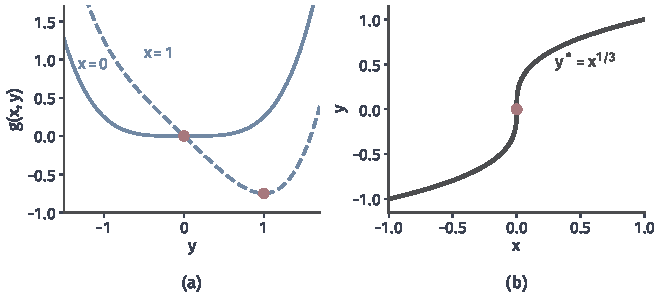
\includegraphics[width=112mm]{figures/05-optimization/07-multiple-criteria-and-nested-optimization/matplotlib/bilevel-singular/figure.pdf}
 \caption{内解唯一但不可微，$g=y^4/4-xy$。(a)$x=0$（实线）的碗底平坦，$H=0$；$x=1$（虚线）的碗底在$y=1$，红点是内解。(b)内解曲线$y^\star=x^{1/3}$连续，红点$x=0$处切线竖直。}
 \label{fig:bilevel-singular}
\end{BookInlineFigure}

\subsection{分支切换}
\label{sec:bilevel-switching}

内层非凸时，几个局部极小点可能并存，谁是全局最优随$\bm{x}$改变。局部分支一直光滑，全局选解却可能在某处跳到另一条分支上。

\paragraph{两个碗交换优劣}
构造一个可以手算的内层，它由两个抛物线取下包络：
\begin{equation}
 g(x,y)=\min\Bigl\{\frac12(y-1-x)^2-x,\ \ \frac12(y+1-x)^2+x\Bigr\}.
 \label{eq:bilevel-two-wells}
\end{equation}

令两式相等并化简，可知两条抛物线始终在$y=0$处相交，那里是两个碗之间的山脊。山脊不在碗底，所以每个碗底附近$g$就是一条光滑的抛物线，定理~\ref{thm:bilevel-local-branch}适用。第一个碗的碗底$y_+(x)=x+1$在$x>-1$时位于山脊右侧，第二个碗的碗底$y_-(x)=x-1$在$x<1$时位于山脊左侧。两个碗底的高度分别是
\[
 g(x,y_+(x))=-x,\qquad g(x,y_-(x))=x.
\]

所以$x>0$时右边的碗更低，$x<0$时左边的碗更低，$x=0$时打平。全局解集是
\[
 S(x)=\begin{cases}
 \{x-1\}, & x<0,\\
 \{-1,\ 1\}, & x=0,\\
 \{x+1\}, & x>0.
 \end{cases}
\]

图~\ref{fig:bilevel-switch-inner}(a)画了三个$x$处的$g$，(b)画了解曲线。全局选解在$x=0$处从下面一条分支跳到上面一条，两条分支本身都连续穿过$x=0$。

\begin{BookInlineFigure}
 \centering
 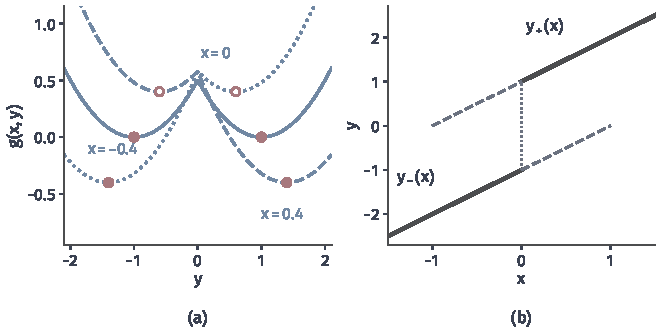
\includegraphics[width=112mm]{figures/05-optimization/07-multiple-criteria-and-nested-optimization/matplotlib/bilevel-switch-inner/figure.pdf}
 \caption{两个内层极小点交换优劣，$g$由式~\eqref{eq:bilevel-two-wells}定义。(a)$x=-0.4,0,0.4$时的$g$，红色实心点是全局极小点，空心点是非全局的局部极小点。(b)深灰粗线是全局内解，灰色虚线是仍为局部极小点、但已不是全局最优的分支延续，点线标出$x=0$处的跳变。}
 \label{fig:bilevel-switch-inner}
\end{BookInlineFigure}

\paragraph{外层目标跟着跳}
取外层目标$F=\frac12(y-\frac12)^2$。沿两条分支的外层值分别是
\[
 \Phi_+(x)=\frac12\Bigl(x+\frac12\Bigr)^2,\qquad\Phi_-(x)=\frac12\Bigl(x-\frac32\Bigr)^2.
\]

全局选解的外层值在$x>0$时是$\Phi_+$，在$x<0$时是$\Phi_-$。在$x=0$处从左极限$9/8$跳到右极限$1/8$，$\Phi$在这里甚至不连续。乐观模型在$x=0$选$y=1$，值为$1/8$；悲观模型选$y=-1$，值为$9/8$。

\paragraph{算法实际追踪的是哪一条}
现在假定外层用梯度下降，内层每次从上一轮的解继续求解。这种\term{热启动}（warm start）使内层一直留在右边的碗里。若沿分支用光滑公式，外层迭代是
\[
 x^{(t+1)}=x^{(t)}-\eta\,\Phi_+'(x^{(t)})=x^{(t)}-\eta\Bigl(x^{(t)}+\frac12\Bigr).
\]

从$x^{(0)}=0.8$出发，取$\eta=0.3$，迭代穿过$x=0$，一路收敛到$x=-\frac12$，此时外层值看上去是$0$。这是图~\ref{fig:bilevel-switch-phi}中的绿色路径。

可是$x=-\frac12$时右边的碗已经不是全局最优了。真正的内解在左边的碗里，$y_-(-\frac12)=-\frac32$，真实的外层值是
\[
 \Phi_-\Bigl(-\frac12\Bigr)=\frac12\Bigl(-\frac12-\frac32\Bigr)^2=2.
\]

算法报告的$0$和真实的$2$之间差了一条红色点线的距离，而算法运行中没有任何量发出警告，因为沿局部分支一切都光滑。

\begin{BookInlineFigure}
 \centering
 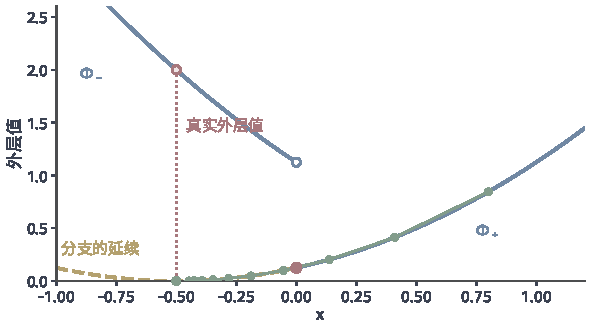
\includegraphics[width=100mm]{figures/05-optimization/07-multiple-criteria-and-nested-optimization/matplotlib/bilevel-switch-phi/figure.pdf}
 \caption{全局选解的外层值在切换点跳变，$F=\frac12(y-\frac12)^2$。蓝线是全局选解的外层值，$x=0$处的空心点是左极限$9/8$，红点是右极限$1/8$，也是乐观模型在$x=0$的值。黄色虚线是分支$\Phi_+$越过切换点后的延续，绿色路径是沿这条分支的外层梯度下降，它停在$x=-1/2$。红色空心点是此处真实的外层值$2$。}
 \label{fig:bilevel-switch-phi}
\end{BookInlineFigure}

表~\ref{tab:bilevel-three-derivatives}分清这里出现的三个“导数”。切换点处不能继续套用同一个光滑公式，这个公式求的是局部分支的导数，在切换点那一边它不再描述全局选解。

\begin{BookInlineTable}
 \centering
 \begin{tabular}{lll}
  \toprule
  对象 & 例中$x=-0.1$处 & 成立范围\\
  \midrule
  局部分支导数$\Phi_+'$ & $0.4$ & 分支存续的区间\\
  全局选解导数$\Phi_-'$ & $-1.6$ & 不含切换点的区间\\
  算法返回的导数 & 取决于碗的选择 & 取决于初值、热启动\\
  \bottomrule
 \end{tabular}
 \caption{分支切换时要区分的三种导数。例中$x=-0.1$时全局内解在左边的碗，热启动的算法却可能仍在右边的碗。}
 \label{tab:bilevel-three-derivatives}
\end{BookInlineTable}

\section{隐式微分}
\label{sec:bilevel-implicit}

在定理~\ref{thm:bilevel-local-branch}成立的分支上，怎样计算外层目标的导数？关键的观察是，求导只需要当前解点处的局部关系。至于这个解是怎样迭代得到的，算法走过了多少步，都不进入公式，也不必保存。

\subsection{超梯度}
\label{sec:bilevel-hypergradient}

设$\hat{\bm{y}}(\bm{x})$是所追踪的分支，外层目标为$\Phi(\bm{x})=F(\bm{x},\hat{\bm{y}}(\bm{x}))$。若内解唯一且满足定理~\ref{thm:bilevel-strong-convex-map}，这条分支就是$\bm{y}^\star(\bm{x})$。$\Phi$对$\bm{x}$的梯度称为\termalias{超梯度-hypergradient}{超梯度}（hypergradient）。“超”在这里指外层，与第~\ref{chap:penalty-multiplier-methods}章凹函数的超梯度（supergradient）是两回事。

\paragraph{主要思想：把响应接到外层}
由链式法则，$\Phi$的梯度由两部分组成：
\[
 \nabla\Phi=\nabla_{\bm{x}}F+\bm{D}^{\top}\nabla_{\bm{y}}F.
\]
第一项是直接作用，第二项是响应。把式~\eqref{eq:bilevel-branch-derivative}代入第二项，并利用$\bm{H}$对称，得到
\[
 \bm{D}^{\top}\nabla_{\bm{y}}F=-\bm{B}^{\top}\bm{H}^{-1}\nabla_{\bm{y}}F.
\]

这个式子不必先算出$\bm{H}^{-1}\bm{B}$这个$d\times n$矩阵。先解一个以$\nabla_{\bm{y}}F$为右端的方程，得到的向量再乘$\bm{B}^{\top}$即可。

\begin{theorem}[隐式超梯度]
\label{thm:bilevel-hypergradient}
设定理~\ref{thm:bilevel-local-branch}的条件成立，$F$在$(\bm{x}_0,\bm{y}_0)$附近连续可微。则$\Phi(\bm{x})=F(\bm{x},\hat{\bm{y}}(\bm{x}))$连续可微，且
\begin{equation}
 \nabla\Phi=\nabla_{\bm{x}}F-\bm{B}^{\top}\bm{v},
 \qquad\bm{H}\bm{v}=\nabla_{\bm{y}}F,
 \label{eq:bilevel-hypergradient}
\end{equation}
其中所有导数都在$(\bm{x},\hat{\bm{y}}(\bm{x}))$处取值。
\end{theorem}

\begin{proof}
$\hat{\bm{y}}$连续可微，$F$连续可微，由链式法则$\Phi$连续可微，其梯度是上面的两项之和。$\bm{H}$正定，所以方程$\bm{H}\bm{v}=\nabla_{\bm{y}}F$有唯一解，即$\bm{v}=\bm{H}^{-1}\nabla_{\bm{y}}F$，代入即得式~\eqref{eq:bilevel-hypergradient}。
\end{proof}

式~\eqref{eq:bilevel-hypergradient}中的$\bm{H}\bm{v}=\nabla_{\bm{y}}F$称为\term{伴随方程}（adjoint equation）。用这种方法求超梯度的做法称为\term{隐式微分}（implicit differentiation），因为内解没有显式公式，导数是从定义它的方程中得出的。

\paragraph{$\bm{v}$是内层梯度的价格}
$\bm{v}$有一个直接的含义。设想把驻点方程改成$\nabla_{\bm{y}}g=\bm{\varepsilon}$，也就是给内层梯度一点小扰动。内解移动$\bm{H}^{-1}\bm{\varepsilon}$，外层值变化约为
\[
 \langle\nabla_{\bm{y}}F,\bm{H}^{-1}\bm{\varepsilon}\rangle=\langle\bm{v},\bm{\varepsilon}\rangle.
\]
所以$\bm{v}$是内层梯度每单位扰动在外层的价格，含义和约束乘子作为影子价格相同。

$\bm{x}$改变$\Delta\bm{x}$时，内层梯度在原来的解点偏移$\bm{B}\Delta\bm{x}$，内解要把这份偏移抵消掉，相当于对内层施加了$-\bm{B}\Delta\bm{x}$的扰动。价格乘以扰动量，就得到响应项$-\langle\bm{B}^{\top}\bm{v},\Delta\bm{x}\rangle$。这个价格只在一阶范围内有效，$\Delta\bm{x}$大了或分支切换了，它就不再准确。

图~\ref{fig:bilevel-adjoint-chain}把这条因果链画了出来。上面一行顺着原因往下算，要带着$n$个方向的$\Delta\bm{x}$走完全程。下面一行从外层往回算，只带一个向量。标量外层目标、很多外层变量时，后者便宜得多。

\begin{BookInlineFigure}
 \centering
 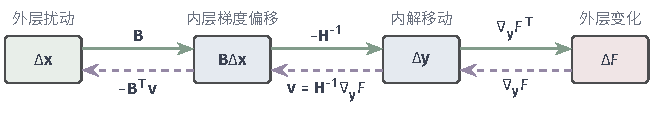
\includegraphics[width=110.6mm]{figures/05-optimization/07-multiple-criteria-and-nested-optimization/tikz/bilevel-adjoint-chain/figure.pdf}
 \caption{超梯度的因果链。绿色实线从外层扰动算到外层变化，每个方向$\Delta\bm{x}$算一次。紫色虚线从外层梯度往回算，一次得到全部分量的梯度，$\bm{v}$是内层梯度偏移的价格。}
 \label{fig:bilevel-adjoint-chain}
\end{BookInlineFigure}

\paragraph{手算核对}
对正则拟合例~\eqref{eq:bilevel-ridge}，在$x=1$处，各量为
\[
 y^\star=\frac32,\qquad H=1+x=2,\qquad B=y^\star=\frac32,\qquad\partial_yF=y^\star-1=\frac12.
\]

解伴随方程，得到
\[
 v=\frac{\partial_yF}{H}=\frac14.
\]

$F$不含$x$，所以由式~\eqref{eq:bilevel-hypergradient}，
\[
 \Phi'(1)=0-Bv=-\frac38.
\]

直接对$\Phi$求导来核对。由链式法则，
\[
 \Phi'(x)=(y^\star-1)\,\frac{\mathrm{d}y^\star}{\mathrm{d}x},
\]
在$x=1$处等于$\frac12\times(-\frac34)=-\frac38$，两者相同。同样可算出$\Phi'(0)=-6$；在$x=2$处$\partial_yF=0$，$v=0$，$\Phi'(2)=0$，这正是最小点。

\paragraph{第二项不能丢}
这个例子里$\nabla_{\bm{x}}F=0$。如果只对$F$求偏导，也就是把$y$固定住，得到的斜率处处是$0$，结论将是$x$不用调整。图~\ref{fig:bilevel-hypergrad-tangent}比较了这两条线。忽略响应项，求的是“固定内解时的偏导数”，并不是双层目标的导数。

\begin{BookInlineFigure}
 \centering
 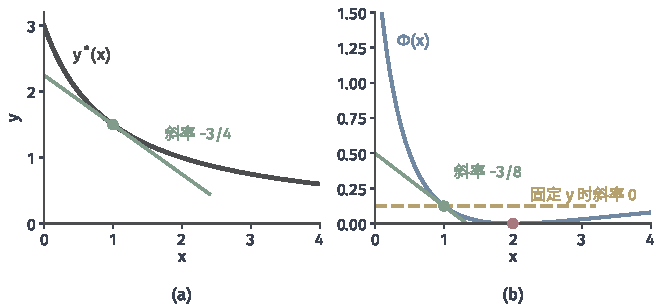
\includegraphics[width=112mm]{figures/05-optimization/07-multiple-criteria-and-nested-optimization/matplotlib/bilevel-hypergrad-tangent/figure.pdf}
 \caption{正则拟合例中$x=1$处的导数。(a)内解曲线的切线，斜率是$\mathrm{d}y^\star/\mathrm{d}x=-3/4$。(b)$\Phi$的切线（绿）斜率是超梯度$-3/8$；黄色虚线是把$y$固定在$y^\star(1)$时的外层函数，斜率为$0$。红点是$\Phi$的最小点。}
 \label{fig:bilevel-hypergrad-tangent}
\end{BookInlineFigure}

\paragraph{与极小极大的联系}
式~\eqref{eq:bilevel-hypergradient}也说明了表~\ref{tab:bilevel-vs-minimax}的最后一行。若$F=-g$，内解处$\nabla_{\bm{y}}F=-\nabla_{\bm{y}}g=\bm{0}$，于是$\bm{v}=\bm{0}$，超梯度退化为$\nabla_{\bm{x}}F$。内解的移动对外层值只有二阶影响，这就是第~\ref{chap:minimax-optimization}章和第~\ref{chap:parametric-sensitivity}章的包络关系。一般的双层问题没有这种抵消，响应项必须计算。

\subsection{线性方程求解}
\label{sec:bilevel-linear-solve}

$d$很大时$\bm{H}$存不下，更不用说求逆。本小节要解决的问题是：怎样只用$\bm{H}$与向量的乘积解伴随方程，以及这个方程解得不准会造成多大的超梯度误差。

\paragraph{主要思想：只用矩阵—向量积}
解$\bm{H}\bm{v}=\nabla_{\bm{y}}F$的迭代法只需要反复计算$\bm{H}\bm{u}$。这个乘积不需要$\bm{H}$的元素，它是内层梯度沿$\bm{u}$方向的方向导数：
\begin{equation}
 \bm{H}\bm{u}=\frac{\mathrm{d}}{\mathrm{d}s}\nabla_{\bm{y}}g(\bm{x},\bm{y}+s\bm{u})\Big|_{s=0}.
 \label{eq:bilevel-hvp}
\end{equation}

这称为\term{Hessian向量积}（Hessian-vector product）。用自动求导时，它的代价是梯度计算的常数倍，也可以用内层梯度的差分近似。$\bm{B}^{\top}\bm{v}$同样如此，它是标量$\langle\nabla_{\bm{y}}g,\bm{v}\rangle$（固定$\bm{v}$）对$\bm{x}$的梯度。

$\bm{H}$对称正定时，共轭梯度法是自然的选择，算法的推导可参考\BookChapterRef{chap:krylov-methods}{卷二第15章“Krylov子空间法”}。第~$k$步用到的量都按下面的递推得到，$\alpha^{(k)}$和$\beta^{(k)}$在本小节里表示共轭梯度法自己的系数：
\begin{equation}
 \begin{gathered}
 \alpha^{(k)}=\frac{\lVert\bm{r}^{(k)}\rVert_2^2}{\langle\bm{d}^{(k)},\bm{H}\bm{d}^{(k)}\rangle},\qquad
 \bm{v}^{(k+1)}=\bm{v}^{(k)}+\alpha^{(k)}\bm{d}^{(k)},\\
 \bm{r}^{(k+1)}=\bm{r}^{(k)}-\alpha^{(k)}\bm{H}\bm{d}^{(k)},\\
 \beta^{(k)}=\frac{\lVert\bm{r}^{(k+1)}\rVert_2^2}{\lVert\bm{r}^{(k)}\rVert_2^2},\qquad
 \bm{d}^{(k+1)}=\bm{r}^{(k+1)}+\beta^{(k)}\bm{d}^{(k)}.
 \end{gathered}
 \label{eq:bilevel-cg}
\end{equation}

\paragraph{计算过程}
下面用二维内层走一遍全过程。内层是带二次惩罚的最小二乘，外层把结果和目标点比较：
\[
 g(x,\bm{y})=\frac12\lVert\bm{A}\bm{y}-\bm{b}\rVert_2^2+\frac{x}{2}\lVert\bm{y}\rVert_2^2,\qquad F(\bm{y})=\frac12\lVert\bm{y}-\bm{c}\rVert_2^2.
\]

数据取为
\[
 \bm{A}=\begin{bmatrix}1&1\\0&1\end{bmatrix},\qquad
 \bm{b}=\begin{bmatrix}3\\1\end{bmatrix},\qquad
 \bm{c}=\begin{bmatrix}0\\2\end{bmatrix}.
\]

\needspace{6\baselineskip}
\paragraph{变量}
\begin{itemize}
 \item 内解$\bm{y}\in\mathbb{R}^d$，事先由内层算法得到。
 \item 伴随向量的迭代值$\bm{v}^{(k)}\in\mathbb{R}^d$，残差$\bm{r}^{(k)}=\nabla_{\bm{y}}F-\bm{H}\bm{v}^{(k)}$，搜索方向$\bm{d}^{(k)}\in\mathbb{R}^d$。
 \item 超梯度估计$\hat{\bm{\gamma}}^{(k)}\in\mathbb{R}^n$，把式~\eqref{eq:bilevel-hypergradient}中的$\bm{v}$换成$\bm{v}^{(k)}$得到。
\end{itemize}

\paragraph{初始化}
先在当前$\bm{x}$处得到内解，计算外层梯度，并置$\bm{v}^{(0)}=\bm{0}$，$\bm{r}^{(0)}=\bm{d}^{(0)}=\nabla_{\bm{y}}F$。

例中取$x=1$。$\bm{H}=\bm{A}^{\top}\bm{A}+x\bm{I}$，解$\bm{H}\bm{y}=\bm{A}^{\top}\bm{b}$得到内解，于是
\[
 \bm{H}=\begin{bmatrix}2&1\\1&3\end{bmatrix},\qquad
 \bm{y}=\begin{bmatrix}1\\1\end{bmatrix},\qquad
 \bm{r}^{(0)}=\bm{y}-\bm{c}=\begin{bmatrix}1\\-1\end{bmatrix}.
\]
$\bm{H}$的两个特征值都为正，共轭梯度法适用。内层梯度对$x$的导数是$\bm{y}$，所以$\bm{B}=\bm{y}$，$\nabla_xF=0$。

\needspace{6\baselineskip}
\paragraph{每轮更新}
\begin{enumerate}
 \item 计算$\bm{H}\bm{d}^{(k)}$，按式~\eqref{eq:bilevel-cg}得到$\alpha^{(k)}$，更新$\bm{v}$和$\bm{r}$。

 例中第一轮，$\bm{H}\bm{d}^{(0)}=(1,-2)$，于是
 \[
  \alpha^{(0)}=\frac{2}{3},\qquad
  \bm{v}^{(1)}=\frac23\begin{bmatrix}1\\-1\end{bmatrix},\qquad
  \bm{r}^{(1)}=\frac13\begin{bmatrix}1\\1\end{bmatrix}.
 \]
 此时的超梯度估计是$-\bm{y}^{\top}\bm{v}^{(1)}=0$。

 \item 按式~\eqref{eq:bilevel-cg}计算$\beta^{(k)}$，更新搜索方向。

 例中第一轮，
 \[
  \beta^{(0)}=\frac{2/9}{2}=\frac19,\qquad
  \bm{d}^{(1)}=\frac13\begin{bmatrix}1\\1\end{bmatrix}+\frac19\begin{bmatrix}1\\-1\end{bmatrix}=\frac29\begin{bmatrix}2\\1\end{bmatrix}.
 \]

 例中第二轮，先算矩阵—向量积和分母：
 \[
  \bm{H}\bm{d}^{(1)}=\frac{10}{9}\begin{bmatrix}1\\1\end{bmatrix},\qquad\langle\bm{d}^{(1)},\bm{H}\bm{d}^{(1)}\rangle=\frac{20}{27}.
 \]
 于是
 \[
  \alpha^{(1)}=\frac{2/9}{20/27}=\frac{3}{10},\qquad
  \bm{v}^{(2)}=\frac15\begin{bmatrix}4\\-3\end{bmatrix},\qquad
  \bm{r}^{(2)}=\bm{0}.
 \]

 \item 残差范数低于设定精度时停止，否则回到第1步。例中$\bm{r}^{(2)}=\bm{0}$，两步结束。
\end{enumerate}

最终得到$\bm{v}=(4/5,-3/5)$，由式~\eqref{eq:bilevel-hypergradient}，超梯度是
\[
 \Phi'(1)=-\bm{y}^{\top}\bm{v}=-\frac15.
\]

直接验证。由式~\eqref{eq:bilevel-branch-derivative}，内解的导数是
\[
 \frac{\mathrm{d}\bm{y}}{\mathrm{d}x}=-\bm{H}^{-1}\bm{y}=-\frac15\begin{bmatrix}2\\1\end{bmatrix},
\]
它与$\nabla_{\bm{y}}F=(1,-1)$的内积是$-1/5$，结果一致。第一轮的残差非零，超梯度估计是$0$，没有反映出真实的下降方向。这引出了下面的误差分析。

\paragraph{共轭梯度法的前提}
式~\eqref{eq:bilevel-cg}的分母要求$\langle\bm{d},\bm{H}\bm{d}\rangle>0$，这需要$\bm{H}$正定。在局部极小点的分支上这成立，但内层非凸且当前点还没收敛时可能不成立。取$\bm{H}=\operatorname{diag}(1,-1)$，$\bm{r}^{(0)}=(1,1)$，第一步的分母就是$1-1=0$，算法无法进行。这时应先检查所在位置是否还在所说的分支上，再选择适用于不定矩阵的求解方法。

\paragraph{线性残差怎样变成超梯度误差}
设$\tilde{\bm{v}}$是近似解，残差$\bm{r}=\bm{H}\tilde{\bm{v}}-\nabla_{\bm{y}}F$。线性方程的残差很小，并不等于超梯度的误差很小，中间隔着$\bm{H}^{-1}$和$\bm{B}$。

\begin{theorem}[伴随残差的放大]
\label{thm:bilevel-residual-amplification}
设内解精确，$\bm{H}\succeq\mu\bm{I}$，$\tilde{\bm{\gamma}}$是把式~\eqref{eq:bilevel-hypergradient}中的$\bm{v}$换成$\tilde{\bm{v}}$所得的估计，残差$\bm{r}=\bm{H}\tilde{\bm{v}}-\nabla_{\bm{y}}F$。则
\begin{equation}
 \lVert\tilde{\bm{\gamma}}-\nabla\Phi\rVert_2\leq\frac{\lVert\bm{B}\rVert_2}{\mu}\,\lVert\bm{r}\rVert_2.
 \label{eq:bilevel-residual-amplification}
\end{equation}
\end{theorem}

\begin{proof}
由残差的定义，$\tilde{\bm{v}}-\bm{v}=\bm{H}^{-1}\bm{r}$，所以
\[
 \tilde{\bm{\gamma}}-\nabla\Phi=-\bm{B}^{\top}(\tilde{\bm{v}}-\bm{v})=-\bm{B}^{\top}\bm{H}^{-1}\bm{r}.
\]
再用$\lVert\bm{H}^{-1}\rVert_2\leq1/\mu$取范数即得。
\end{proof}

上面例子的第一轮，$\lVert\bm{r}^{(1)}\rVert_2=\sqrt{2}/3\approx0.471$，$\lVert\bm{B}\rVert_2=\sqrt2$，$\bm{H}$的最小特征值是$(5-\sqrt5)/2\approx1.382$。代入式~\eqref{eq:bilevel-residual-amplification}，上界约为$0.482$，实际误差是$0.2$。

式~\eqref{eq:bilevel-residual-amplification}说明，内层越病态，同样的残差放大得越厉害；而且病态也让共轭梯度法收敛更慢。图~\ref{fig:bilevel-cg}中，$\kappa=10$时残差很快下降，超梯度误差跟着下降；$\kappa=1000$时残差下降缓慢，超梯度误差还比残差大几倍到几十倍。内层病态的问题需要把线性方程解得更准，这笔账要算进总成本。

\begin{BookInlineFigure}
 \centering
 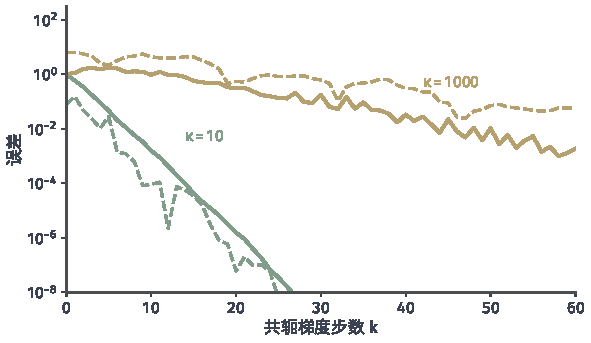
\includegraphics[width=100mm]{figures/05-optimization/07-multiple-criteria-and-nested-optimization/matplotlib/bilevel-cg/figure.pdf}
 \caption{共轭梯度法解伴随方程的收敛，$d=60$，$\bm{H}$的特征值在$[1/\kappa,1]$上对数均匀分布，$\bm{B}$、$\nabla_{\bm{y}}F$是固定种子下的随机单位向量。实线是残差范数，虚线是超梯度的绝对误差。绿色$\kappa=10$，黄色$\kappa=1000$。}
 \label{fig:bilevel-cg}
\end{BookInlineFigure}

\paragraph{另一种近似：Neumann级数}
若$0<\alpha<2/\lambda_{\max}(\bm{H})$，矩阵$\bm{I}-\alpha\bm{H}$的谱半径小于$1$，$\bm{H}^{-1}$可以展开为级数：
\begin{equation}
 \bm{H}^{-1}=\alpha\sum_{k=0}^{\infty}(\bm{I}-\alpha\bm{H})^k.
 \label{eq:bilevel-neumann}
\end{equation}
只取前$\ell$项，就得到一种只用Hessian向量积的近似。它收敛比共轭梯度法慢，但第~\ref{sec:bilevel-truncated}小节会看到，它恰好就是截断展开的极限形式。

\subsection{约束内层}
\label{sec:bilevel-constrained-inner}

内层有约束时，内解满足的不再是驻点方程，$\bm{H}$的位置也要换成整个KKT系统。本小节要解决的问题是：什么时候这样做是对的，以及哪些情况下根本不存在经典的导数。

\paragraph{主要思想：对活动的KKT方程求导}
$g$已用作内层目标，这里把内层约束写成$c_i(\bm{x},\bm{y})\leq0$（$i=1,\ldots,m$）和$h_j(\bm{x},\bm{y})=0$（$j=1,\ldots,p$），Lagrange函数是
\begin{equation}
 \mathcal{L}(\bm{x},\bm{y},\bm{\lambda},\bm{\nu})=g+\sum_{i=1}^{m}\lambda_ic_i+\sum_{j=1}^{p}\nu_jh_j.
 \label{eq:bilevel-lagrangian}
\end{equation}

第~\ref{chap:constrained-optimality}章的KKT条件和第~\ref{chap:parametric-sensitivity}章的敏感性定理告诉我们：在基准KKT点处，若线性无关约束资格（LICQ）、严格互补和二阶充分条件成立，则存在邻域内的连续可微分支，活动集$A$在分支上保持不变，分支上的点都是严格局部极小点。

把活动不等式当成等式，记活动不等式与等式的总数为$a+p$，定义四个矩阵。前两个是$\mathcal{L}$的二阶导数：
\[
 \bm{W}=\nabla^2_{\bm{y}\bm{y}}\mathcal{L},\qquad\bm{B}_{\mathcal{L}}=\nabla^2_{\bm{y}\bm{x}}\mathcal{L}.
\]
另外两个来自约束：$\bm{J}$的行是活动约束和等式约束对$\bm{y}$的梯度，$\bm{E}$的行是它们对$\bm{x}$的梯度。KKT矩阵为
\begin{equation}
 \bm{K}=\begin{bmatrix}\bm{W}&\bm{J}^{\top}\\\bm{J}&\bm{0}\end{bmatrix}.
 \label{eq:bilevel-kkt-matrix}
\end{equation}

\begin{theorem}[约束内层的隐式超梯度]
\label{thm:bilevel-constrained-hypergradient}
设在基准KKT点处$g,c_i,h_j$二阶连续可微，LICQ、严格互补与二阶充分条件成立，$F$连续可微。则$\Phi(\bm{x})=F(\bm{x},\hat{\bm{y}}(\bm{x}))$在基准点附近连续可微，且
\begin{equation}
 \nabla\Phi=\nabla_{\bm{x}}F-\bm{B}_{\mathcal{L}}^{\top}\bm{v}-\bm{E}^{\top}\bm{w},
 \qquad
 \bm{K}\begin{bmatrix}\bm{v}\\\bm{w}\end{bmatrix}=\begin{bmatrix}\nabla_{\bm{y}}F\\\bm{0}\end{bmatrix}.
 \label{eq:bilevel-constrained-hypergradient}
\end{equation}
\end{theorem}

\begin{proof}
由第~\ref{chap:parametric-sensitivity}章的不等式约束解导数定理，$\bm{K}$可逆，分支的Jacobian矩阵$\bm{D}$与乘子导数$\bm{D}_{\bm{w}}$满足
\[
 \bm{K}\begin{bmatrix}\bm{D}\\\bm{D}_{\bm{w}}\end{bmatrix}=-\begin{bmatrix}\bm{B}_{\mathcal{L}}\\\bm{E}\end{bmatrix}.
\]

取$(\bm{v},\bm{w})$为式~\eqref{eq:bilevel-constrained-hypergradient}中方程的解，并用$\bm{K}$对称，得到
\[
 \bm{D}^{\top}\nabla_{\bm{y}}F=\begin{bmatrix}\bm{D}\\\bm{D}_{\bm{w}}\end{bmatrix}^{\top}\bm{K}\begin{bmatrix}\bm{v}\\\bm{w}\end{bmatrix}=-\bm{B}_{\mathcal{L}}^{\top}\bm{v}-\bm{E}^{\top}\bm{w}.
\]
代入第~\ref{sec:bilevel-hypergradient}小节开头的链式法则即得。
\end{proof}

\paragraph{预算例}
外层变量取预算$x=\tau$，内层沿用第~\ref{chap:parametric-sensitivity}章的预算二次问题的主要部分，外层想让配置接近另一个点：
\[
 \begin{aligned}
 g(\bm{y})&=\frac12(y_1-2)^2+\frac12(y_2-1)^2,\quad c(\tau,\bm{y})=y_1+y_2-\tau\leq0,\\
 F(\bm{y})&=\frac12(y_1-2)^2+\frac12(y_2-2)^2.
 \end{aligned}
\]

在$\tau=2$处约束活动，内解和乘子是$\bm{y}=(3/2,1/2)$，$\lambda=1/2>0$，严格互补成立。各块矩阵和右端为
\[
 \bm{W}=\bm{I},\quad\bm{J}=\begin{bmatrix}1&1\end{bmatrix},\quad\bm{B}_{\mathcal{L}}=\bm{0},\quad E=-1,\quad\nabla_{\bm{y}}F=\begin{bmatrix}-1/2\\-3/2\end{bmatrix}.
\]

式~\eqref{eq:bilevel-constrained-hypergradient}的方程组写开是
\[
 v_1+w=-\frac12,\qquad v_2+w=-\frac32,\qquad v_1+v_2=0.
\]

前两式相加并用第三式，得$w=-1$，于是$v_1=1/2$，$v_2=-1/2$。代入超梯度公式，
\[
 \Phi'(2)=-E\,w=-1.
\]

直接核对：约束活动时$\bm{y}=((1+\tau)/2,(\tau-1)/2)$，它对$\tau$的导数是$(1/2,1/2)$，与$\nabla_{\bm{y}}F$的内积是$-1$。图~\ref{fig:bilevel-kkt-kink}(a)的绿线是这条解路径。

\paragraph{公式失效的情形}
活动集变化时导数会断。预算例中$\lambda=(3-\tau)/2$，到$\tau=3$时乘子降为零，严格互补失效，内解停在理想点$(2,1)$。外层值的左导数由$(\tau-4)/2$给出，在$\tau=3$处等于$-1/2$；$\tau>3$时外层值是常数，右导数是$0$。这就是图~\ref{fig:bilevel-kkt-kink}(b)的折点，经典的导数在此不存在。

\begin{BookInlineFigure}
 \centering
 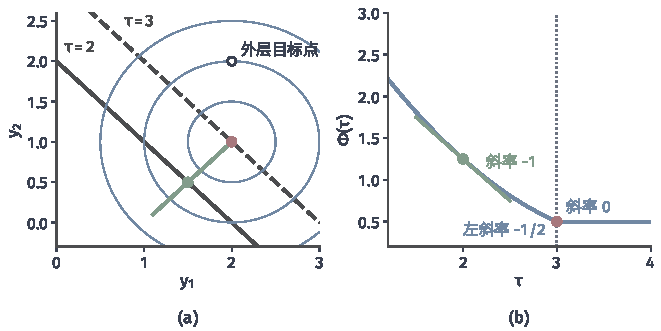
\includegraphics[width=112mm]{figures/05-optimization/07-multiple-criteria-and-nested-optimization/matplotlib/bilevel-kkt-kink/figure.pdf}
 \caption{约束内层的预算例。(a)蓝色等高线属于内层目标，红点是无约束最优$(2,1)$，深灰实线和虚线分别是$\tau=2$和$\tau=3$的预算线，绿线是内解随$\tau$移动的路径，绿点是$\tau=2$的解，空心点是外层目标点$(2,2)$。(b)外层值$\Phi(\tau)$，绿色切线在$\tau=2$处斜率$-1$；红点$\tau=3$处活动集改变，左斜率$-1/2$，右斜率$0$。}
 \label{fig:bilevel-kkt-kink}
\end{BookInlineFigure}

$\bm{K}$奇异时公式不能使用，但内解不一定不可微。取内层$\min\frac12(y-2)^2$，约束$y\leq\tau$和$2y\leq2\tau$是同一条约束的两种写法。在$\tau=1$处两者都活动，$\bm{J}$的两行成比例，LICQ失效，$\bm{K}$奇异，乘子也不唯一。而内解$y=\min\{\tau,2\}$在$\tau=1$附近的导数是$1$，完全正常。

还有一种常见的错误，是把$\bm{H}$换成$\bm{W}$，仍用式~\eqref{eq:bilevel-hypergradient}。预算例中$\bm{W}=\bm{I}$，$\bm{B}_{\mathcal{L}}=\bm{0}$，这样算出的解导数是零向量，而真实导数是$(1/2,1/2)$。约束的作用全在$\bm{J}$和$\bm{E}$里，只换一个矩阵等于把约束的响应丢掉了。

\section{迭代展开}
\label{sec:bilevel-unrolling}

隐式微分依赖“内层已经到了解点”这一前提。如果真正运行的是有限步算法，也可以直接对算法的输出求导。于是要问：怎样对$\bm{y}^{(T)}(\bm{x})$求导，这样算出的量和隐式导数有什么关系？这种做法称为\term{迭代展开}（unrolled differentiation）。

设内层的一步更新写成
\begin{equation}
 \bm{y}^{(t+1)}=\bm{\Psi}_t(\bm{y}^{(t)},\bm{x}),\qquad t=0,\ldots,T-1.
 \label{eq:bilevel-update}
\end{equation}
梯度下降取$\bm{\Psi}_t=\bm{y}-\alpha\nabla_{\bm{y}}g$，这些更新规则本身的性质在第~\ref{chap:first-order-methods}章讨论，下面只处理沿更新传播导数时新增的对象。

\subsection{完整展开}
\label{sec:bilevel-full-unroll}

\paragraph{主要思想：把算法看成复合函数}
$\bm{y}^{(T)}$是$\bm{x}$经过$T$层复合得到的函数，对它求导只需要反复使用链式法则。图~\ref{fig:bilevel-unroll-graph}是$T=2$的计算图，$\bm{x}$进入每一步更新，所以每一层都要算一次它的影响。

\begin{BookInlineFigure}
 \centering
 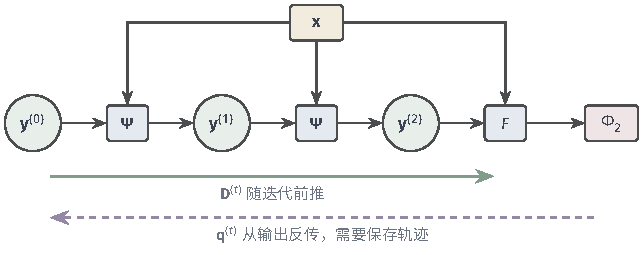
\includegraphics[width=108.9mm]{figures/05-optimization/07-multiple-criteria-and-nested-optimization/tikz/bilevel-unroll-graph/figure.pdf}
 \caption{$T=2$时的展开计算图。圆圈是内层状态，方框$\bm{\Psi}$是一步更新，$\bm{x}$进入每步更新和外层目标。绿色实线表示前向传播Jacobian矩阵$\bm{D}^{(t)}$，紫色虚线表示从外层往回传播向量$\bm{q}^{(t)}$。}
 \label{fig:bilevel-unroll-graph}
\end{BookInlineFigure}

记$\bm{D}^{(t)}\in\mathbb{R}^{d\times n}$为$\bm{y}^{(t)}$对$\bm{x}$的Jacobian矩阵，并记一步更新的两个偏导数：
\[
 \bm{A}^{(t)}=\frac{\partial\bm{\Psi}_t}{\partial\bm{y}}\in\mathbb{R}^{d\times d},\qquad
 \bm{C}^{(t)}=\frac{\partial\bm{\Psi}_t}{\partial\bm{x}}\in\mathbb{R}^{d\times n}.
\]
两者都在$(\bm{y}^{(t)},\bm{x})$处取值。对梯度下降，$\bm{A}^{(t)}=\bm{I}-\alpha\bm{H}^{(t)}$，$\bm{C}^{(t)}=-\alpha\bm{B}^{(t)}$，其中$\bm{H}^{(t)}$、$\bm{B}^{(t)}$是在当前迭代点算出的二阶导数。

对式~\eqref{eq:bilevel-update}两边关于$\bm{x}$求导。$\bm{y}^{(t)}$本身依赖$\bm{x}$，所以
\begin{equation}
 \bm{D}^{(t+1)}=\bm{A}^{(t)}\bm{D}^{(t)}+\bm{C}^{(t)}.
 \label{eq:bilevel-forward}
\end{equation}

有限步目标的梯度由链式法则得到：
\begin{equation}
 \nabla\Phi_T=\nabla_{\bm{x}}F+(\bm{D}^{(T)})^{\top}\nabla_{\bm{y}}F,
 \label{eq:bilevel-finite-gradient}
\end{equation}
其中$F$的导数在$(\bm{x},\bm{y}^{(T)})$处取值。这是精确的导数，只不过它是$\Phi_T$的导数。

\paragraph{主要思想：反向累积}
式~\eqref{eq:bilevel-forward}要带着一个$d\times n$矩阵走完全程，$n$很大时存不下。把递推展开，得到
\[
 \bm{D}^{(T)}=\sum_{t=0}^{T-1}\bm{A}^{(T-1)}\cdots\bm{A}^{(t+1)}\bm{C}^{(t)}+\bm{A}^{(T-1)}\cdots\bm{A}^{(0)}\bm{D}^{(0)}.
\]

式~\eqref{eq:bilevel-finite-gradient}只需要这个矩阵的转置与一个向量的乘积，可以从左边的向量开始依次向右乘。令$\bm{q}^{(T)}=\nabla_{\bm{y}}F$，从$t=T-1$到$0$计算
\begin{equation}
 \bm{h}\leftarrow\bm{h}+(\bm{C}^{(t)})^{\top}\bm{q}^{(t+1)},\qquad
 \bm{q}^{(t)}=(\bm{A}^{(t)})^{\top}\bm{q}^{(t+1)}.
 \label{eq:bilevel-reverse}
\end{equation}
$\bm{h}$的初值是$\nabla_{\bm{x}}F$，循环结束后再加上$(\bm{D}^{(0)})^{\top}\bm{q}^{(0)}$，结果就是$\nabla\Phi_T$。

两种顺序保存的东西不同。前向传播保存$\bm{D}^{(t)}$，不用保存轨迹。反向累积只保存向量，但$\bm{A}^{(t)}$、$\bm{C}^{(t)}$要在$\bm{y}^{(t)}$处计算，所以必须把整条轨迹保存下来，或者重新算出来。

\paragraph{计算过程}
用正则拟合例在$x=0$处计算$\Phi_3'(0)$，内层取$y^{(0)}=0$，$\alpha=1/2$。

\needspace{6\baselineskip}
\paragraph{变量}
\begin{itemize}
 \item 迭代点$y^{(t)}$，前向时的导数$D^{(t)}$，这里$d=n=1$，它们都是数。
 \item 一步更新的偏导数$A^{(t)}=1-\alpha(1+x)$，$C^{(t)}=-\alpha y^{(t)}$。
 \item 反向时的累积量$q^{(t)}$和结果$h$。
\end{itemize}

\paragraph{初始化}
初值不依赖$x$，所以$D^{(0)}=0$。例中$x=0$，于是$A^{(t)}=1/2$，$C^{(t)}=-y^{(t)}/2$。

\needspace{6\baselineskip}
\paragraph{每轮更新}
\begin{enumerate}
 \item 前向：更新$y^{(t+1)}$，并按式~\eqref{eq:bilevel-forward}更新$D^{(t+1)}$。

 例中第一轮$D^{(1)}=\frac12\cdot0-\frac12\cdot0=0$，第二轮用$y^{(1)}=3/2$，第三轮用$y^{(2)}=9/4$，各轮结果为
 \[
  y^{(1)},y^{(2)},y^{(3)}=\frac32,\ \frac94,\ \frac{21}{8};\qquad
  D^{(1)},D^{(2)},D^{(3)}=0,\ -\frac34,\ -\frac32.
 \]

 \item 走完$T$步后由式~\eqref{eq:bilevel-finite-gradient}得到梯度。

 例中$\partial_yF=y^{(3)}-1=13/8$，$\partial_xF=0$，于是
 \[
  \Phi_3'(0)=D^{(3)}\cdot\frac{13}{8}=-\frac{39}{16}.
 \]

 \item 反向：若改用反向累积，从$q^{(3)}=13/8$、$h=0$开始按式~\eqref{eq:bilevel-reverse}回算。

 例中$t=2$时$C^{(2)}=-9/8$，$t=1$时$C^{(1)}=-3/4$，$t=0$时$C^{(0)}=0$，各轮结果为
 \[
  h:\ -\frac{117}{64},\ -\frac{156}{64},\ -\frac{156}{64};\qquad
  q^{(2)},q^{(1)},q^{(0)}=\frac{13}{16},\ \frac{13}{32},\ \frac{13}{64}.
 \]
\end{enumerate}

最终$h=-156/64=-39/16$，与前向结果相同。这个数是$\Phi_3$的精确导数，而$\Phi$的导数是$-6$，两者相差很大，都是正确的导数，只是对应不同的目标。

\paragraph{初始化、动量与不可微更新}
若初值依赖$\bm{x}$，$\bm{D}^{(0)}$不为零，它的贡献必须保留。用上一轮解作热启动时，严格说初值也依赖过去的$\bm{x}$，把这一项丢掉就是在计算另一个量的导数。

算法含动量时，一步更新依赖不止一个迭代点。例如重球法的更新是
\[
 \bm{y}^{(t+1)}=\bm{y}^{(t)}-\alpha\nabla_{\bm{y}}g+\omega(\bm{y}^{(t)}-\bm{y}^{(t-1)}),
\]
要把$\bm{z}^{(t)}=(\bm{y}^{(t)},\bm{y}^{(t-1)})$作为完整状态，式~\eqref{eq:bilevel-forward}和式~\eqref{eq:bilevel-reverse}对$\bm{z}$成立。只对$\bm{y}$求导会漏掉上一步的影响。

邻近迭代的情况不同。第~\ref{chap:nonsmooth-composite-optimization}章的软阈值映射是分段光滑的，在分段的边界处没有经典导数，展开的公式只在迭代不落在边界上时才成立。

表~\ref{tab:bilevel-unroll-cost}比较两种传播顺序的代价，规模变量是内层维数$d$、外层维数$n$和步数$T$。反向累积的存储可以用\term{检查点}（checkpointing）减少：每隔$k$步保存一次状态，回算时从最近的检查点重算，$k\approx\sqrt{T}$时存储降到约$\sqrt{T}$个状态，代价是多大约一倍的计算量。

\begin{BookInlineTable}
 \centering
 \begin{tabular}{lll}
  \toprule
  做法 & 存储 & 每步主要运算\\
  \midrule
  前向传播 & $O(dn)$ & $n$次Hessian向量积\\
  反向累积 & $O(Td)$ & 一次Hessian向量积\\
  隐式微分 & $O(d)$ & 每次线性迭代一次积\\
  \bottomrule
 \end{tabular}
 \caption{三种超梯度计算的代价。存储只计迭代中保存的向量，隐式微分要求内层已解到解点附近，迭代次数由线性方程的精度决定。}
 \label{tab:bilevel-unroll-cost}
\end{BookInlineTable}

\subsection{截断展开}
\label{sec:bilevel-truncated}

保存整条轨迹太贵时，常见的做法是只反传末尾$\ell$步。这和少跑几步内层是两件不同的事。

\paragraph{两种缩短}
第一种，把内层步数从$T$减到$T'$。目标函数换成了$\Phi_{T'}$，它的导数依然精确，只是目标变了。第二种，内层仍跑满$T$步，反向只回到$t=T-\ell$，相当于在式~\eqref{eq:bilevel-reverse}中提前停止，并丢掉更早的响应。目标还是$\Phi_T$，算出的是它导数的近似。

\begin{theorem}[截断反传的误差]
\label{thm:bilevel-truncation}
设$\tilde{\bm{D}}$是把递推~\eqref{eq:bilevel-forward}中$\bm{D}^{(T-\ell)}$换成零后得到的矩阵。则
\begin{equation}
 \lVert(\bm{D}^{(T)}-\tilde{\bm{D}})^{\top}\nabla_{\bm{y}}F\rVert_2\leq
 \Bigl\lVert\prod_{t=T-\ell}^{T-1}\bm{A}^{(t)}\Bigr\rVert_2\lVert\bm{D}^{(T-\ell)}\rVert_2\lVert\nabla_{\bm{y}}F\rVert_2.
 \label{eq:bilevel-truncation}
\end{equation}
其中连乘按$t$从大到小自左向右排列。
\end{theorem}

\begin{proof}
从第$T-\ell$步开始展开递推，得到
\[
 \bm{D}^{(T)}=\sum_{t=T-\ell}^{T-1}\bm{A}^{(T-1)}\cdots\bm{A}^{(t+1)}\bm{C}^{(t)}+\bm{A}^{(T-1)}\cdots\bm{A}^{(T-\ell)}\bm{D}^{(T-\ell)}.
\]
$\tilde{\bm{D}}$恰好是右端的求和部分，差就是第二项。转置、右乘$\nabla_{\bm{y}}F$，再取范数即得。
\end{proof}

内层是收缩迭代时，连乘随$\ell$几何衰减，所以末尾的若干步已经包含了大部分信息。

\paragraph{正则拟合例中的比较}
$x=0$时$A=1/2$。取$T=20$，$y^{(t)}$已非常接近$3$，$\partial_yF\approx2$，只反传$\ell$步得到的结果约为
\[
 -6\bigl(1-2^{-\ell}\bigr).
\]
$\ell=1$时约为$-3$，$\ell=3$时约为$-5.25$。图~\ref{fig:bilevel-unroll-derivative}(b)中的绿线是这组值，黄线是真正只跑$T=\ell$步的$\Phi_\ell'(0)$，依次为$0,-15/16,-39/16$等。两者随$\ell$都趋向$-6$，黄线要慢得多，因为它不仅少反传，还因内层没跑够而用错了$y$。

\begin{BookInlineFigure}
 \centering
 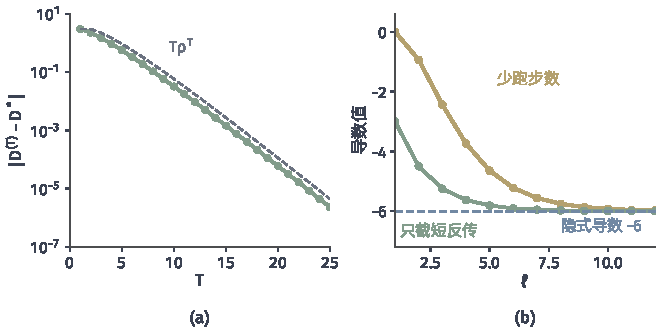
\includegraphics[width=112mm]{figures/05-optimization/07-multiple-criteria-and-nested-optimization/matplotlib/bilevel-unroll-derivative/figure.pdf}
 \caption{展开导数与隐式导数的关系，正则拟合例，$x=0$，$\alpha=1/2$。(a)绿线是导数误差$|D^{(T)}-D^\star|=3(T+1)2^{-T}$，虚线是定理~\ref{thm:bilevel-unroll-limit}型的参考界。(b)黄线是真实步数为$T=\ell$的完整展开导数，绿线是$T=20$、只反传$\ell$步的结果，蓝色虚线是隐式导数$-6$。}
 \label{fig:bilevel-unroll-derivative}
\end{BookInlineFigure}

截断后的向量一般不是$\Phi_T$的梯度，也不保证是它的下降方向。设误差向量为$\bm{e}$，真实梯度为$\bm{\gamma}$。只有在$\lVert\bm{e}\rVert_2<\lVert\bm{\gamma}\rVert_2$时才能由
\[
 \langle\bm{\gamma}+\bm{e},\bm{\gamma}\rangle\geq\lVert\bm{\gamma}\rVert_2\bigl(\lVert\bm{\gamma}\rVert_2-\lVert\bm{e}\rVert_2\bigr)>0
\]
断定它仍是下降方向。

\paragraph{与隐式微分的联系}
若内层已收敛，每一步的$\bm{A}^{(t)}$、$\bm{C}^{(t)}$都等于解点处的值$\bm{I}-\alpha\bm{H}$和$-\alpha\bm{B}$，反传$\ell$步给出
\[
 \nabla_{\bm{x}}F-\bm{B}^{\top}\Bigl[\alpha\sum_{k=0}^{\ell-1}(\bm{I}-\alpha\bm{H})^k\Bigr]\nabla_{\bm{y}}F.
\]
方括号正是式~\eqref{eq:bilevel-neumann}的前$\ell$项，所以截断反传相当于用Neumann级数的部分和代替$\bm{H}^{-1}$。

\subsection{极限关系}
\label{sec:bilevel-limit}

既然两种路线在内层收敛时形式一致，自然要问：$T\to\infty$时，展开的导数是否趋于隐式导数。答案是在收缩性等条件下成立，而只有迭代点收敛是不够的。

\begin{theorem}[展开导数的收敛]
\label{thm:bilevel-unroll-limit}
固定$\bm{x}$，内层用梯度下降，步长$\alpha\leq1/L_g$。设沿迭代路径和$\bm{y}^\star$处有$\mu\bm{I}\preceq\bm{H}\preceq L_g\bm{I}$，且存在常数$L_H,L_B$，使这些点上$\bm{H}$、$\bm{B}$关于$\bm{y}$分别$L_H$、$L_B$—Lipschitz。记
\begin{equation}
 \begin{gathered}
 \rho=1-\alpha\mu,\qquad\bm{D}^\star=-\bm{H}_\star^{-1}\bm{B}_\star,\\
 e_0=\lVert\bm{y}^{(0)}-\bm{y}^\star\rVert_2,\qquad c=\alpha(L_H\lVert\bm{D}^\star\rVert_2+L_B)e_0.
 \end{gathered}
 \label{eq:bilevel-unroll-constants}
\end{equation}
若迭代满足
\begin{equation}
 \lVert\bm{y}^{(t)}-\bm{y}^\star\rVert_2\leq\rho^te_0,
 \label{eq:bilevel-unroll-linear}
\end{equation}
则
\begin{equation}
 \lVert\bm{D}^{(T)}-\bm{D}^\star\rVert_2\leq\rho^T\lVert\bm{D}^{(0)}-\bm{D}^\star\rVert_2+cT\rho^{T-1}.
 \label{eq:bilevel-unroll-limit}
\end{equation}
\end{theorem}

\begin{proof}
先说明$\bm{D}^\star$是极限递推的不动点。把$\bm{A}_\star=\bm{I}-\alpha\bm{H}_\star$、$\bm{C}_\star=-\alpha\bm{B}_\star$代入，得到
\[
 \bm{A}_\star\bm{D}^\star+\bm{C}_\star=\bm{D}^\star-\alpha\bm{H}_\star\bm{D}^\star-\alpha\bm{B}_\star=\bm{D}^\star.
\]

记$\bm{E}^{(t)}=\bm{D}^{(t)}-\bm{D}^\star$，用递推式减去不动点方程，并在中间加减$\bm{A}^{(t)}\bm{D}^\star$，得到
\[
 \bm{E}^{(t+1)}=\bm{A}^{(t)}\bm{E}^{(t)}+(\bm{A}^{(t)}-\bm{A}_\star)\bm{D}^\star+(\bm{C}^{(t)}-\bm{C}_\star).
\]

条件$\alpha\leq1/L_g$使$\bm{A}^{(t)}$的特征值落在$[0,\rho]$，所以$\lVert\bm{A}^{(t)}\rVert_2\leq\rho$。由Lipschitz条件和式~\eqref{eq:bilevel-unroll-linear}，后两项的范数之和不超过$c\rho^t$，于是
\[
 \lVert\bm{E}^{(t+1)}\rVert_2\leq\rho\lVert\bm{E}^{(t)}\rVert_2+c\rho^t.
\]

对$T$归纳。$T=0$时式~\eqref{eq:bilevel-unroll-limit}成立。若对$T$成立，代入上式，得到
\[
 \lVert\bm{E}^{(T+1)}\rVert_2\leq\rho^{T+1}\lVert\bm{E}^{(0)}\rVert_2+cT\rho^{T}+c\rho^T=\rho^{T+1}\lVert\bm{E}^{(0)}\rVert_2+c(T+1)\rho^{T}.
\]
这就是$T+1$时的结论。
\end{proof}

收缩率$\rho$控制衰减，多出的因子$T$来自迭代点误差在每一层的累积。把结果代入式~\eqref{eq:bilevel-finite-gradient}，当$\nabla_{\bm{x}}F$、$\nabla_{\bm{y}}F$关于$\bm{y}$连续时，$\nabla\Phi_T\to\nabla\Phi$。

\paragraph{手算核对}
正则拟合例在$x=0$处，$\mu=L_g=1$，$\rho=1/2$，$L_H=0$，$L_B=1$，$e_0=3$，$c=3/2$，$\lVert D^{(0)}-D^\star\rVert=3$。式~\eqref{eq:bilevel-unroll-limit}的右端是$3\cdot2^{-T}+3T\cdot2^{-T}$。

另一方面，对式~\eqref{eq:bilevel-ridge-finite}直接求导，得到$D^{(T)}=-3+3(T+1)2^{-T}$，误差恰好等于
\[
 \lvert D^{(T)}-D^\star\rvert=3(T+1)2^{-T}.
\]
上界在这个例子里取等号。

\paragraph{点列收敛不够}
内层点列收敛这个事实本身，不足以交换求导与极限。设内层目标是$g=\frac12(y-x)^2$，$y^\star(x)=x$，某个带扰动的内层算法输出
\[
 y^{(T)}(x)=x+\frac{\sin(Tx)}{T}.
\]

对所有$x$，误差不超过$1/T$，点列一致收敛到内解。可是$\mathrm{d}y^{(T)}/\mathrm{d}x=1+\cos(Tx)$，在$x=0$处恒等于$2$，而隐式导数是$1$。误差的幅度在缩小，它的振荡频率却在增加，导数记录的恰恰是后者。定理~\ref{thm:bilevel-unroll-limit}用收缩和导数的Lipschitz条件排除了这种情形。

收缩一旦失去，结论也无从谈起。正则拟合例中$\alpha=1/2$时$q=(1-x)/2$，$x\geq3$时$\lvert q\rvert\geq1$，迭代不收敛，$\Phi_T$描述的是一个发散算法的输出。而且，固定的短展开并不自动给出真实双层目标的梯度：$T=2$时的导数$-15/16$与$-6$相差甚远。

\section{单层重述}
\label{sec:bilevel-single-level}

前两节都把$\Phi$当作函数，靠内层求解和求导来下降。另一种思路是不把内层嵌套着解，而把“$\bm{y}$确实是内解”写成关于$(\bm{x},\bm{y})$的约束，然后一起最小化外层目标。接下来要弄清：这样的约束有哪些写法，每种写法保留了什么，又失去了什么？

对乐观模型，由式~\eqref{eq:bilevel-optimistic-joint}，这个想法可以直接实现。悲观模型不行：外层目标里夹着一个对解集的$\sup$，把它改成对$\bm{y}$的联合最小化就等于把最坏情况换成了最好情况，它还需要再嵌套一层，不能套用下面的改写。本节只讨论乐观模型。

\subsection{最优性条件重述}
\label{sec:bilevel-kkt-reformulation}

用$\bm{y}$的最优性条件替代“$\bm{y}\in\bm{S}(\bm{x})$”是最直接的做法，内层有约束时这就是KKT条件。

\paragraph{写成一个单层问题}
沿用式~\eqref{eq:bilevel-lagrangian}的记号，把乘子也作为变量，得到下面的问题：
\begin{equation}
 \begin{aligned}
 \min_{\bm{x},\bm{y},\bm{\lambda},\bm{\nu}}\quad&F(\bm{x},\bm{y})\\
 \text{s.t.}\quad&\bm{x}\in\bm{C},\quad\nabla_{\bm{y}}\mathcal{L}=\bm{0},\quad\bm{h}=\bm{0},\\
 &\bm{c}\leq\bm{0},\quad\bm{\lambda}\geq\bm{0},\quad\lambda_ic_i=0,\ i=1,\ldots,m.
 \end{aligned}
 \label{eq:bilevel-mpcc}
\end{equation}
含有$\lambda_ic_i=0$这样的约束的问题称为\term{互补约束规划}（mathematical program with complementarity constraints），简称MPCC。

这样的改写要成立，必须保证KKT条件恰好刻画内层的全局解。KKT条件一般只是局部解的必要条件，下面的定理给出能作此替换的情形。

\begin{theorem}[凸内层的KKT重述]
\label{thm:bilevel-kkt-equivalence}
设对每个$\bm{x}\in\bm{C}$，$g(\bm{x},\cdot)$和$c_i(\bm{x},\cdot)$凸且连续可微，$h_j(\bm{x},\cdot)$仿射，内层满足Slater条件。则对每个$\bm{x}\in\bm{C}$，
\begin{equation}
 \bm{y}\in\bm{S}(\bm{x})\iff\text{存在}(\bm{\lambda},\bm{\nu})\text{使}(\bm{x},\bm{y},\bm{\lambda},\bm{\nu})\text{满足式~\eqref{eq:bilevel-mpcc}的约束}.
 \label{eq:bilevel-kkt-equivalence}
\end{equation}
于是$(\bm{x},\bm{y})$是乐观模型的全局解，当且仅当存在乘子使$(\bm{x},\bm{y},\bm{\lambda},\bm{\nu})$是式~\eqref{eq:bilevel-mpcc}的全局解。
\end{theorem}

\begin{proof}
固定$\bm{x}$。凸问题的KKT点是全局解，这给出“$\Leftarrow$”；Slater条件下凸问题的全局解满足KKT条件，乘子存在，这给出“$\Rightarrow$”。这两个结论见第~\ref{chap:constrained-optimality}章和第~\ref{chap:duality}章。两个问题的目标都只含$(\bm{x},\bm{y})$，可行点的$(\bm{x},\bm{y})$分量又相同，所以全局解的$(\bm{x},\bm{y})$分量也相同。
\end{proof}

定理只对应全局解。局部解的对应要复杂得多：式~\eqref{eq:bilevel-mpcc}的局部解固定了一组乘子，而原问题要比较所有乘子对应的邻近点，乘子不唯一时两者可以不一致。相关反例的构造较长，读者可查阅双层规划的专门文献。

\paragraph{非凸内层的反例}
内层非凸时，KKT点可能根本不是全局解。取无约束内层和外层
\[
 g(y)=\frac14y^4-\frac12y^2,\qquad F(y)=\frac12y^2.
\]

驻点方程$y^3-y=0$的解是$y\in\{-1,0,1\}$。全局解是$y=\pm1$，外层值是$1/2$。可是重述问题只要求驻点方程，它会选$y=0$，外层值是$0$，而$y=0$恰好是内层的局部极大点。

\paragraph{一个凸内层的例子}
取内层$\min_y\frac12(y-x)^2$，约束$y\geq0$，也就是$c=-y\leq0$。外层目标取$F=\frac12(x+1)^2+\frac12(y-1)^2$。内层的KKT条件是
\[
 y-x-\lambda=0,\qquad y\geq0,\qquad\lambda\geq0,\qquad\lambda y=0.
\]

互补条件把可行集分成两支。$\lambda=0$时$y=x\geq0$；$y=0$时$\lambda=-x\geq0$。这就是图~\ref{fig:bilevel-mpcc}(b)的折线，$y^\star(x)=\max\{x,0\}$。

在两支上分别求解。沿$y=x$，$x\geq0$，外层值是$x^2+1$，最小值是$x=0$处的$1$。沿$y=0$，$x\leq0$，外层值是$\frac12(x+1)^2+\frac12$，最小值是$x=-1$处的$\frac12$。全局解是$(x,y)=(-1,0)$。

\paragraph{互补约束为什么难}
图~\ref{fig:bilevel-mpcc}(a)画出了$a\geq0$、$b\geq0$、$ab=0$的可行集，它由两条半轴组成，没有内部，在原点还拐了一个直角。一般非线性规划算法依靠约束资格，而这类可行集恰好破坏它们。

\begin{BookInlineFigure}
 \centering
 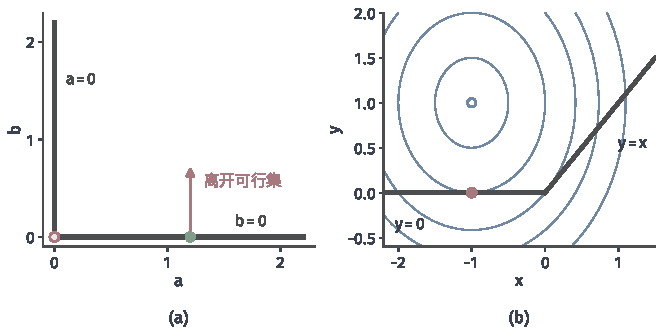
\includegraphics[width=112mm]{figures/05-optimization/07-multiple-criteria-and-nested-optimization/matplotlib/bilevel-mpcc/figure.pdf}
 \caption{互补约束的几何。(a)$a\geq0$、$b\geq0$、$ab=0$的可行集是两条半轴。在绿点处，严格满足不等式$b\geq0$的方向（红箭头）立刻离开可行集；原点处（空心点）拐角使等式约束的梯度为零。(b)内层$\min\frac12(y-x)^2$，$y\geq0$的解图像（深灰折线），蓝色是外层等高线，空心点是外层的无约束最小点$(-1,1)$，红点是双层问题的解$(-1,0)$。}
 \label{fig:bilevel-mpcc}
\end{BookInlineFigure}

\begin{lemma}[互补约束破坏MFCQ]
\label{lem:bilevel-mfcq-fails}
设$m\geq1$。式~\eqref{eq:bilevel-mpcc}的每个可行点都不满足Mangasarian—Fromovitz约束资格（MFCQ）。
\end{lemma}

\begin{proof}
MFCQ要求等式约束的梯度线性无关，并存在方向$\bm{d}$，使它与所有等式约束的梯度正交，且与所有活动不等式约束的梯度内积为负。考虑某一对约束$\lambda_i\geq0$、$c_i\leq0$、$e=\lambda_ic_i=0$，在全部变量构成的空间中，等式的梯度是
\[
 \nabla e=c_i\nabla\lambda_i+\lambda_i\nabla c_i.
\]

若$\lambda_i>0$，$c_i=0$，则$\nabla e=\lambda_i\nabla c_i$。$c_i\leq0$活动，MFCQ要求$\langle\nabla c_i,\bm{d}\rangle<0$，于是$\langle\nabla e,\bm{d}\rangle<0$，与正交矛盾。

若$\lambda_i=0$，$c_i<0$，则$\nabla e=c_i\nabla\lambda_i$。$-\lambda_i\leq0$活动，MFCQ要求$\langle\nabla\lambda_i,\bm{d}\rangle>0$，于是$\langle\nabla e,\bm{d}\rangle<0$，同样矛盾。

若$\lambda_i=c_i=0$，则$\nabla e=\bm{0}$，等式约束的梯度线性相关。三种情形穷尽了可行点的所有可能。
\end{proof}

所以即使内层是凸的，也不能把一般非线性规划的收敛结论直接搬过来，那些结论通常要求某种约束资格。实践中的做法有两类：内层约束不多时枚举互补的分支，每一支是一个正常的问题，但分支数最多是$2^m$；或者把$\lambda_ic_i=0$松弛成$-\lambda_ic_i\leq t$，让$t$逐渐趋于零，松弛问题有内部，但收敛到的点要回到原问题核对。

\subsection{值函数重述}
\label{sec:bilevel-value-reformulation}

最优性条件的重述要靠凸性才能表达全局最优。另一种写法直接比较目标值，不需要内层的结构。

\paragraph{直接比较内层目标值}
定义内层最优值函数
\begin{equation}
 V(\bm{x})=\inf_{\bm{y}\in\bm{Y}(\bm{x})}g(\bm{x},\bm{y}).
 \label{eq:bilevel-value-function}
\end{equation}
$\bm{y}$是内解，当且仅当它内层可行，且它的内层目标值达到了最优值。

\begin{lemma}[值函数重述]
\label{lem:bilevel-value-reformulation}
设$V(\bm{x})$有限。则
\begin{equation}
 \bm{y}\in\bm{S}(\bm{x})\iff\bm{y}\in\bm{Y}(\bm{x})\text{且}g(\bm{x},\bm{y})\leq V(\bm{x}).
 \label{eq:bilevel-value-constraint}
\end{equation}
\end{lemma}

\begin{proof}
若$\bm{y}\in\bm{S}(\bm{x})$，则$\bm{y}$可行且$g(\bm{x},\bm{y})=V(\bm{x})$。反过来，$\bm{y}$可行时必有$g(\bm{x},\bm{y})\geq V(\bm{x})$，再加上不等式$g(\bm{x},\bm{y})\leq V(\bm{x})$，就得到等号，所以$\bm{y}$取得内层最小值。
\end{proof}

引理没有用到任何凸性，所以全局选解这个要求被完整地写了下来。乐观模型因而等价于
\[
 \min_{\bm{x}\in\bm{C},\,\bm{y}\in\bm{Y}(\bm{x})}F(\bm{x},\bm{y})\quad\text{s.t.}\quad g(\bm{x},\bm{y})-V(\bm{x})\leq0.
\]

\paragraph{用正则拟合例计算}
把式~\eqref{eq:bilevel-ridge-solution}代入$g$并化简，得到
\[
 V(x)=\frac{9x}{2(1+x)}.
\]

$g$对$y$是二次函数，二次项系数为$(1+x)/2$，所以
\[
 g(x,y)-V(x)=\frac{1+x}{2}\bigl(y-y^\star(x)\bigr)^2.
\]
约束$g-V\leq0$迫使$y=y^\star(x)$，确实把内解曲线重新写了出来。$V$的导数可以用包络关系求，
\[
 V'(x)=\partial_xg(x,y^\star(x))=\frac12(y^\star)^2=\frac{9}{2(1+x)^2},
\]
它和直接求导的结果相同。

\paragraph{两个困难}
第一，$V$可能不光滑。式~\eqref{eq:bilevel-two-wells}的内层有$V(x)=-\lvert x\rvert$，在切换点$x=0$处有折点，如图~\ref{fig:bilevel-value}(a)。一般地，$V$是一族函数的下确界，切换解的地方就会出现折点。计算$V$本身也要解一次内层问题。

第二，约束本身是退化的。在$\bm{y}\in\bm{Y}(\bm{x})$上总有$g-V\geq0$，所以不存在严格满足$g-V<0$的点，Slater条件永远不成立。上面的例子里更明显：约束函数$\frac{1+x}{2}(y-y^\star)^2$在可行点处的梯度是零向量，它提供不了任何关于如何回到可行集的一阶信息。

\paragraph{松弛之后要重新核对}
常见的处理是把约束放宽成$g-V\leq\varepsilon$，$\varepsilon>0$。这样可行集有了内部，但代价是允许了不是内解的点。

正则拟合例中，$\varepsilon=0.1$时可行集成了内解曲线周围的一条带，它的半宽是$\sqrt{2\varepsilon/(1+x)}$，见图~\ref{fig:bilevel-value}(b)。外层目标在$y=1$处取最小值$0$，带子与直线$y=1$相交的部分全部是松弛问题的解。令$u=1+x$，条件是
\[
 (u-3)^2\leq0.2\,u.
\]

解得$u\in[2.319,3.881]$，即$x\in[1.319,2.881]$。真实的解$x=2$只是其中一点，松弛让最优解从一个点变成了一个区间，最优值也可能偏低。

\begin{BookInlineFigure}
 \centering
 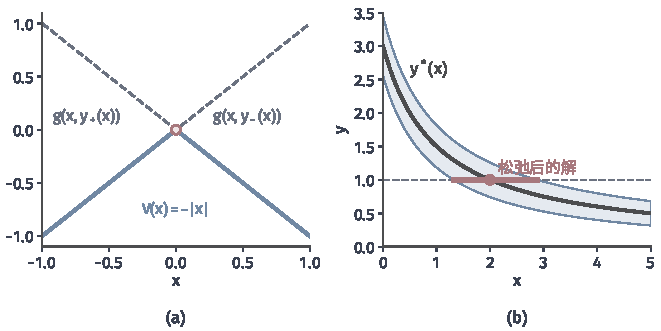
\includegraphics[width=112mm]{figures/05-optimization/07-multiple-criteria-and-nested-optimization/matplotlib/bilevel-value/figure.pdf}
 \caption{值函数重述的两个困难。(a)式~\eqref{eq:bilevel-two-wells}的最优值函数$V(x)=-|x|$（蓝），虚线是沿两条分支的内层值，切换点（空心点）处$V$不可微。(b)正则拟合例的松弛$g-V\leq0.1$：浅蓝带是松弛后的可行集，深灰线是内解，红色线段是带子与$y=1$的交集，即松弛问题的全部最优解；红点是原问题的解$x=2$。}
 \label{fig:bilevel-value}
\end{BookInlineFigure}

罚函数也可以用，把$\rho(g-V)$加进外层目标。有限的$\rho$得到的通常只是近似解。不论松弛还是惩罚，得到的点都要重新检查：内层最优间隙$g-V$有多大，它对应的内解距离有多大，以及改变$\varepsilon$或$\rho$后解是否稳定。

表~\ref{tab:bilevel-reformulations}比较两种重述。

\begin{BookInlineTable}
 \centering
 \begin{tabular}{lll}
  \toprule
  & KKT重述 & 值函数重述\\
  \midrule
  全局等价 & 需凸性与约束资格 & 不需要\\
  新增变量 & 乘子 & 无\\
  主要困难 & 互补约束 & $V$的计算与不光滑\\
  约束资格 & MFCQ处处失效 & Slater永不成立\\
  \bottomrule
 \end{tabular}
 \caption{乐观模型的两种单层重述。悲观模型不能这样改写。}
 \label{tab:bilevel-reformulations}
\end{BookInlineTable}

\section{外层求解}
\label{sec:bilevel-outer}

有了超梯度，外层就可以用前面各章的方法：$\bm{C}$是简单集合时用投影梯度（第~\ref{chap:feasible-iterations}章），变量多而问题光滑时用拟牛顿法（第~\ref{chap:quasi-newton}章），$\Phi$有折点时用非光滑方法（第~\ref{chap:nonsmooth-composite-optimization}章）。选择之前先要确定优化的是哪个目标：真实选解的$\Phi$，还是有限步的$\Phi_T$。

超梯度带着偏差时，外层能保证什么？若把带固定偏差的超梯度当成精确梯度，收敛结论就不成立了。下面按内层、导数、外层的顺序逐级核算。

\subsection{内层误差}
\label{sec:bilevel-inner-error}

内层算法停下时，手里是一个近似解$\hat{\bm{y}}$。这个点离内解有多远，可以用三个量来描述，它们含义不同，需要的计算条件也不同。

\paragraph{三种度量}
固定$\bm{x}$，记所选内解为$\bm{y}^\star$，定义
\[
 \delta=g(\bm{x},\hat{\bm{y}})-g(\bm{x},\bm{y}^\star),\qquad r=\lVert\nabla_{\bm{y}}g(\bm{x},\hat{\bm{y}})\rVert_2,\qquad d=\lVert\hat{\bm{y}}-\bm{y}^\star\rVert_2.
\]

$\delta$是内层目标差距，要知道最优值才能算。$r$是驻点残差，随手可算。$d$是到所选解的距离，通常没法直接算，而超梯度的误差恰恰取决于它。三者只有在特定条件下才能互相控制。

\begin{lemma}[强凸下的互控]
\label{lem:bilevel-inner-measures}
设对固定的$\bm{x}$，$\mu\bm{I}\preceq\nabla^2_{\bm{y}\bm{y}}g\preceq L_g\bm{I}$处处成立。则
\begin{align}
 \mu d&\leq r\leq L_gd,
 \label{eq:bilevel-inner-r}\\
 \frac{\mu}{2}d^2&\leq\delta\leq\frac{L_g}{2}d^2,
 \label{eq:bilevel-inner-delta}\\
 \frac{r^2}{2L_g}&\leq\delta\leq\frac{r^2}{2\mu}.
 \label{eq:bilevel-inner-pl}
\end{align}
\end{lemma}

\begin{proof}
记$\phi=g(\bm{x},\cdot)$，$\bm{e}=\hat{\bm{y}}-\bm{y}^\star$。由$\nabla\phi(\bm{y}^\star)=\bm{0}$和积分形式的中值定理，
\[
 \nabla\phi(\hat{\bm{y}})=\bar{\bm{H}}\bm{e},
\]
其中$\bar{\bm{H}}$是Hessian沿线段的平均，特征值在$[\mu,L_g]$内，这给出式~\eqref{eq:bilevel-inner-r}。

由Taylor公式，
\[
 \delta=\frac12\bm{e}^{\top}\tilde{\bm{H}}\bm{e},
\]
$\tilde{\bm{H}}$的特征值同样在$[\mu,L_g]$内，这给出式~\eqref{eq:bilevel-inner-delta}。

由强凸性，
\[
 \phi(\bm{y}^\star)\geq\phi(\hat{\bm{y}})-rd+\frac{\mu}{2}d^2\geq\phi(\hat{\bm{y}})-\frac{r^2}{2\mu},
\]
第二步是对$d$取最小，这给出式~\eqref{eq:bilevel-inner-pl}的右半。对左半，从$\hat{\bm{y}}$走一步梯度下降$\hat{\bm{y}}-\nabla\phi(\hat{\bm{y}})/L_g$，由下降引理，函数值至少下降$r^2/(2L_g)$，而它不会低于$\phi(\bm{y}^\star)$。
\end{proof}

\paragraph{条件去掉会怎样}
图~\ref{fig:bilevel-inner-measures}对比了强凸的$g=y^2/2$和平坦的$g=y^4/4$。对后者，$r=d^3$，$\delta=d^4/4$。当$d=0.1$时，残差只有$10^{-3}$，目标差距只有$2.5\times10^{-5}$，看上去已经收敛得很好，到解的距离却还有$0.1$。

\begin{BookInlineFigure}
 \centering
 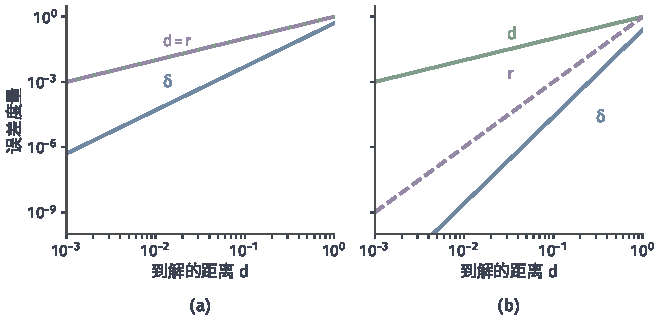
\includegraphics[width=112mm]{figures/05-optimization/07-multiple-criteria-and-nested-optimization/matplotlib/bilevel-inner-measures/figure.pdf}
 \caption{三种内层误差度量随距离$d$的变化，双对数坐标。(a)强凸的$g=y^2/2$：残差$r$（紫色虚线）与$d$（绿）重合，目标差距$\delta$（蓝）是$d^2/2$。(b)平坦的$g=y^4/4$：$r=d^3$，$\delta=d^4/4$，残差和目标差距都远小于到解的距离。}
 \label{fig:bilevel-inner-measures}
\end{BookInlineFigure}

非凸时情况更糟。$r=0$只说明是驻点，它可能是极大点或鞍点。即使是极小点，$d$也必须对着“所选解”算：$\delta$和$r$再小，也无法说明算法是否在正确的那个碗里。

\paragraph{热启动的得失}
外层变化不大时，内层从上一轮解继续，可以省去大量迭代，这是热启动的好处。第~\ref{sec:bilevel-switching}小节也展示了它的代价：它会一直追踪同一条局部分支，穿过切换点也不察觉。热启动减少重复求解，但不能免除全局选解的核对；内层非凸时，需要定期从不同初值重解内层，比较内层目标值。

\subsection{导数误差}
\label{sec:bilevel-derivative-error}

超梯度的误差有几个来源：内解没解准，所有二阶导数都算在错误的点上；伴随方程没解准；或者反传被截断。它们对外层方向的影响要分开看。

\paragraph{两项误差的分解}
记$\hat{\bm{H}}$、$\hat{\bm{B}}$是在$\hat{\bm{y}}$处计算的矩阵，$\bm{f}(\bm{y})=\nabla_{\bm{y}}F(\bm{x},\bm{y})$，并简写$\hat{\bm{f}}=\bm{f}(\hat{\bm{y}})$、$\bm{f}_\star=\bm{f}(\bm{y}^\star)$。设$\tilde{\bm{v}}$是伴随方程的近似解，残差和超梯度估计分别是
\begin{equation}
 \bm{r}_{\bm{v}}=\hat{\bm{H}}\tilde{\bm{v}}-\hat{\bm{f}},\qquad\hat{\bm{\gamma}}=\nabla_{\bm{x}}F(\bm{x},\hat{\bm{y}})-\hat{\bm{B}}^{\top}\tilde{\bm{v}}.
 \label{eq:bilevel-hypergradient-estimate}
\end{equation}

\begin{theorem}[超梯度误差的分解]
\label{thm:bilevel-hypergradient-error}
固定$\bm{x}$，设在$\bm{y}^\star$和$\hat{\bm{y}}$之间：$\bm{H}\succeq\mu\bm{I}$，$\lVert\hat{\bm{B}}\rVert_2\leq M_B$，$\lVert\bm{f}_\star\rVert_2\leq M_F$；$\nabla_{\bm{x}}F$、$\nabla_{\bm{y}}F$关于$\bm{y}$是$L_F$—Lipschitz的，$\bm{H}$、$\bm{B}$关于$\bm{y}$分别是$L_H$、$L_B$—Lipschitz的。记$d=\lVert\hat{\bm{y}}-\bm{y}^\star\rVert_2$。则
\begin{equation}
 \lVert\hat{\bm{\gamma}}-\nabla\Phi(\bm{x})\rVert_2\leq C_d\,d+\frac{M_B}{\mu}\lVert\bm{r}_{\bm{v}}\rVert_2,
 \label{eq:bilevel-hypergradient-error}
\end{equation}
其中常数为
\begin{equation}
 C_d=L_F+\frac{L_BM_F}{\mu}+\frac{M_B}{\mu}\Bigl(L_F+\frac{L_HM_F}{\mu}\Bigr).
 \label{eq:bilevel-hypergradient-constant}
\end{equation}
\end{theorem}

\begin{proof}
记$\bm{v}^\star=\bm{H}_\star^{-1}\bm{f}_\star$，由$\bm{H}_\star\succeq\mu\bm{I}$得$\lVert\bm{v}^\star\rVert_2\leq M_F/\mu$。在$\bm{B}$的差上加减一项，把误差拆成三部分：
\[
 \begin{aligned}
 \hat{\bm{\gamma}}-\nabla\Phi={}&\bigl[\nabla_{\bm{x}}F(\bm{x},\hat{\bm{y}})-\nabla_{\bm{x}}F(\bm{x},\bm{y}^\star)\bigr]\\
 &-(\hat{\bm{B}}-\bm{B}_\star)^{\top}\bm{v}^\star-\hat{\bm{B}}^{\top}(\tilde{\bm{v}}-\bm{v}^\star).
 \end{aligned}
\]

前两部分的范数分别不超过$L_Fd$和$L_BM_Fd/\mu$。第三部分要估计$\tilde{\bm{v}}-\bm{v}^\star$。由残差的定义和$\bm{f}_\star=\bm{H}_\star\bm{v}^\star$，得到
\[
 \hat{\bm{H}}(\tilde{\bm{v}}-\bm{v}^\star)=\bm{r}_{\bm{v}}+(\hat{\bm{f}}-\bm{f}_\star)-(\hat{\bm{H}}-\bm{H}_\star)\bm{v}^\star.
\]

两边乘$\hat{\bm{H}}^{-1}$并取范数，得到
\[
 \lVert\tilde{\bm{v}}-\bm{v}^\star\rVert_2\leq\frac{1}{\mu}\Bigl(\lVert\bm{r}_{\bm{v}}\rVert_2+L_Fd+\frac{L_HM_F}{\mu}d\Bigr).
\]
再乘$\lVert\hat{\bm{B}}\rVert_2\leq M_B$，三部分相加即得式~\eqref{eq:bilevel-hypergradient-error}。
\end{proof}

右端第一项由内层距离$d$负责，第二项由伴随残差负责，两者互不替代。只把$d$压小而不解准伴随方程，或者反过来，都会停在另一项决定的误差水平上。迭代展开时第二项换成式~\eqref{eq:bilevel-truncation}的截断误差。这些结论都要有相应的稳定性条件：$\mu$变小，所有系数都变大；$\bm{H}$奇异时上界不成立。

\paragraph{手算一次}
正则拟合例在$x=1$处，$y^\star=3/2$，$\Phi'(1)=-3/8$。设内层只解到$\hat{y}=1.4$，$d=0.1$，这时$\hat{H}=2$，$\hat{B}=1.4$，$\partial_yF=0.4$。伴随方程精确解是$\hat{v}=0.2$，超梯度估计和误差分别是
\[
 \hat{\gamma}=-0.28,\qquad\lvert\hat{\gamma}-\Phi'(1)\rvert=0.095.
\]

若再把伴随方程解错，取$\tilde{v}=0.15$，残差是$r_v=2\times0.15-0.4=-0.1$，则
\[
 \tilde{\gamma}=-0.21,\qquad\lvert\tilde{\gamma}-\Phi'(1)\rvert=0.165.
\]

代入式~\eqref{eq:bilevel-hypergradient-constant}。这里$L_F=L_B=1$，$L_H=0$，$\mu=2$，$M_F=1/2$，$M_B=1.4$，所以$C_d=1.95$，式~\eqref{eq:bilevel-hypergradient-error}的右端是
\[
 1.95\times0.1+0.7\times0.1=0.265.
\]
它确实是$0.165$的上界。

\paragraph{用数值实验看两项}
图~\ref{fig:bilevel-error-grid}用一个$d=30$的正则最小二乘内层，同时改变内层步数$K$和共轭梯度步数$k$。(a)中$k$固定时，增加$K$只能把误差压到某个平台，平台高度由$k$决定。(b)中$K$固定时，增加$k$也只能压到由$K$决定的平台。两个旋钮要一起拧，单独加大其中一个是浪费。

\begin{BookInlineFigure}
 \centering
 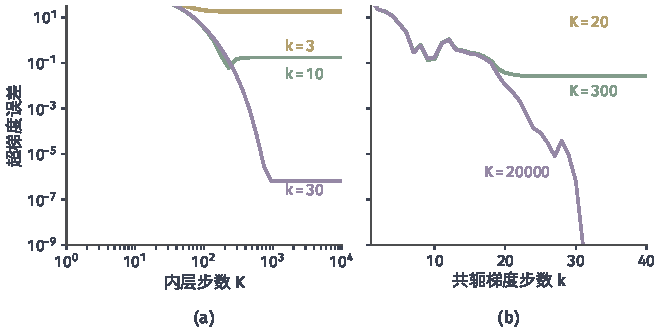
\includegraphics[width=112mm]{figures/05-optimization/07-multiple-criteria-and-nested-optimization/matplotlib/bilevel-error-grid/figure.pdf}
 \caption{超梯度误差的两个来源。内层是$d=30$的正则最小二乘，$x=0.05$，$\kappa\approx48$，数据由固定种子生成；内层用从零出发的梯度下降，步长$1/L_g$，伴随方程用共轭梯度法。(a)固定$k=3,10,30$，误差随内层步数$K$的变化。(b)固定$K=20,300,20000$，误差随共轭梯度步数$k$的变化。}
 \label{fig:bilevel-error-grid}
\end{BookInlineFigure}

\subsection{外层误差}
\label{sec:bilevel-outer-error}

最后把内层和导数的误差接到外层。本小节要解决的问题是：外层迭代用的是有偏差的超梯度，最终能保证什么，以及什么时候应该停下。

\paragraph{主要思想：偏差决定下限}
外层最简单的情形是无约束的梯度下降，用带误差$\bm{e}^{(t)}$的估计代替真实梯度：
\[
 \hat{\bm{\gamma}}^{(t)}=\nabla\Phi(\bm{x}^{(t)})+\bm{e}^{(t)}.
\]
下面的定理说明，偏差会直接进入驻定精度。

\begin{theorem}[带误差的外层梯度下降]
\label{thm:bilevel-inexact-outer}
设$\Phi$有下界$\Phi_{\inf}$，梯度在含迭代点的区域上$L_{\Phi}$—Lipschitz。迭代
\begin{equation}
 \bm{x}^{(t+1)}=\bm{x}^{(t)}-\frac{1}{L_{\Phi}}\hat{\bm{\gamma}}^{(t)}
 \label{eq:bilevel-outer-update}
\end{equation}
满足
\begin{equation}
 \min_{0\leq t<T}\lVert\nabla\Phi(\bm{x}^{(t)})\rVert_2^2\leq\frac{2L_{\Phi}\bigl(\Phi(\bm{x}^{(0)})-\Phi_{\inf}\bigr)}{T}+\frac1T\sum_{t=0}^{T-1}\lVert\bm{e}^{(t)}\rVert_2^2.
 \label{eq:bilevel-inexact-outer}
\end{equation}
\end{theorem}

\begin{proof}
记$\bm{\gamma}=\nabla\Phi(\bm{x}^{(t)})$，$\hat{\bm{\gamma}}=\bm{\gamma}+\bm{e}$，略去上标。由下降引理，
\[
 \Phi(\bm{x}^{(t+1)})\leq\Phi(\bm{x}^{(t)})-\frac{1}{L_{\Phi}}\langle\bm{\gamma},\hat{\bm{\gamma}}\rangle+\frac{1}{2L_{\Phi}}\lVert\hat{\bm{\gamma}}\rVert_2^2.
\]

利用恒等式
\[
 2\langle\bm{\gamma},\hat{\bm{\gamma}}\rangle=\lVert\bm{\gamma}\rVert_2^2+\lVert\hat{\bm{\gamma}}\rVert_2^2-\lVert\bm{e}\rVert_2^2,
\]
$\lVert\hat{\bm{\gamma}}\rVert_2^2$项正好抵消，得到
\[
 \Phi(\bm{x}^{(t+1)})\leq\Phi(\bm{x}^{(t)})-\frac{1}{2L_{\Phi}}\lVert\bm{\gamma}\rVert_2^2+\frac{1}{2L_{\Phi}}\lVert\bm{e}\rVert_2^2.
\]

对$t$从$0$到$T-1$求和，用$\Phi(\bm{x}^{(T)})\geq\Phi_{\inf}$，两边乘$2L_{\Phi}/T$，再用最小值不超过平均值即得。
\end{proof}

若偏差始终约为$\varepsilon$，式~\eqref{eq:bilevel-inexact-outer}右端第二项约为$\varepsilon^2$，不随$T$减小，这个上界只能保证$\lVert\nabla\Phi\rVert_2$降到$\varepsilon$的量级。要得到收敛，内层精度必须随外层进展提高，比如让$\sum_t\lVert\bm{e}^{(t)}\rVert_2^2$有限，这时第二项按$1/T$衰减。

这正对应图~\ref{fig:bilevel-outer-bias}。正则拟合例取$\eta=1$，从$x^{(0)}=1$出发，内层跑固定的$K$步后代入隐式公式。$K=2$时迭代收敛到$x=5/3$，这里$\hat{y}=1$，估计的超梯度为零，真实梯度却是$-27/512$。$K$增大时偏差缩小但不消失，只有$K$随$t$增长时才收敛到$x=2$。

\begin{BookInlineFigure}
 \centering
 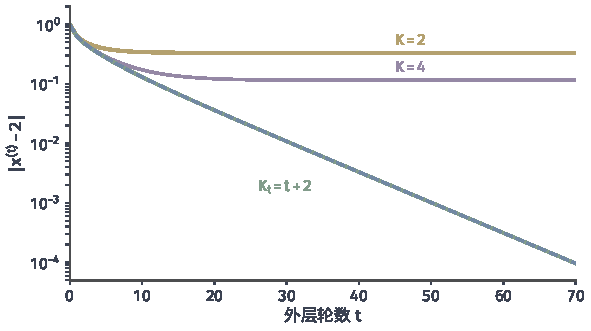
\includegraphics[width=100mm]{figures/05-optimization/07-multiple-criteria-and-nested-optimization/matplotlib/bilevel-outer-bias/figure.pdf}
 \caption{外层迭代误差$\lvert x^{(t)}-2\rvert$，正则拟合例，外层步长$\eta=1$，$x^{(0)}=1$，内层每轮从$y^{(0)}=0$跑$K$步后用隐式公式。黄线$K=2$、紫线$K=4$停在偏差决定的平台，绿线$K_t=t+2$与精确内解（蓝色虚线）几乎重合，持续收敛。}
 \label{fig:bilevel-outer-bias}
\end{BookInlineFigure}

\paragraph{计算过程}
把整个外层循环在这个例子上走几轮，内层步数取$K_t=t+2$。

\needspace{6\baselineskip}
\paragraph{变量}
\begin{itemize}
 \item 外层迭代点$x^{(t)}$，外层步长$\eta$。
 \item 内层输出$\hat{y}$，内层残差$r=(1+x)\hat{y}-3$。
 \item 伴随解$v$，超梯度估计$\hat{\gamma}$。
\end{itemize}

\paragraph{初始化}
例中$x^{(0)}=1$，$\eta=1$。正则拟合例在$x\geq1$上$\lvert\Phi''\rvert\leq15/16$，步长$\eta=1$略小于$1/L_{\Phi}=16/15$，定理~\ref{thm:bilevel-inexact-outer}的证明同样适用，只需把$L_{\Phi}$换成$1/\eta$。

\needspace{6\baselineskip}
\paragraph{每轮更新}
\begin{enumerate}
 \item 内层从$y^{(0)}=0$运行$K_t$步，由式~\eqref{eq:bilevel-ridge-finite}得到$\hat{y}$，并记录残差$r$。

 例中第一轮$x=1$，$q=0$，$\hat{y}=3/2$，残差为$0$。

 \item 解伴随方程，由式~\eqref{eq:bilevel-hypergradient-estimate}得到超梯度估计。

 例中$H=1+x$，$\partial_yF=\hat{y}-1$，$B=\hat{y}$，第一轮的结果是
 \[
  v=\frac{\hat{y}-1}{1+x}=\frac14,\qquad\hat{\gamma}=-\hat{y}v=-\frac38.
 \]

 \item 更新外层变量：$x^{(t+1)}=x^{(t)}-\eta\hat{\gamma}$。

 例中第一轮得到$x^{(1)}=11/8=1.375$。后面几轮的数值见表~\ref{tab:bilevel-outer-rounds}。
\end{enumerate}

\begin{BookInlineTable}
 \centering
 \begin{tabular}{rrrrrrr}
  \toprule
  $t$ & $K_t$ & $x^{(t)}$ & $\hat{y}$ & $r$ & $\hat{\gamma}$ & $\Phi'$\\
  \midrule
  $0$ & $2$ & $1.0000$ & $1.5000$ & $0.0000$ & $-0.3750$ & $-0.3750$\\
  $1$ & $3$ & $1.3750$ & $1.2715$ & $0.0198$ & $-0.1453$ & $-0.1400$\\
  $2$ & $4$ & $1.5203$ & $1.1849$ & $-0.0137$ & $-0.0869$ & $-0.0899$\\
  $3$ & $5$ & $1.6072$ & $1.1536$ & $0.0077$ & $-0.0680$ & $-0.0665$\\
  $4$ & $6$ & $1.6752$ & $1.1197$ & $-0.0044$ & $-0.0501$ & $-0.0509$\\
  \bottomrule
 \end{tabular}
 \caption{正则拟合例的外层循环，$\eta=1$，内层步数$K_t=t+2$。最后一列是在当前$x^{(t)}$处的真实超梯度。}
 \label{tab:bilevel-outer-rounds}
\end{BookInlineTable}

最终$x^{(t)}$趋于$x=2$。表中$\hat{\gamma}$与真实导数的差随内层残差缩小，这就是定理~\ref{thm:bilevel-hypergradient-error}所说的情况。

\paragraph{报告什么、何时停止}
外层的停止不能只看损失曲线，下面四项要分别检查，其中任何一项不达标都不能得出结论。

\begin{itemize}
 \item 外层可行性：$\bm{x}\in\bm{C}$是否成立，$\bm{x}$是否在$\operatorname{dom}\bm{S}$内，也就是内层确实有解。
 \item 外层驻定：有约束时用投影梯度的残差，无约束时用$\lVert\hat{\bm{\gamma}}\rVert_2$，并以估计的偏差为基准；$\lVert\hat{\bm{\gamma}}\rVert_2$低于偏差水平时继续迭代已没有依据。
 \item 内层误差：驻点残差或目标差距；非凸时再比较不同初值下的内层目标值。
 \item 导数误差：伴随残差或截断长度，并可用$\Phi$的中心差分抽查几个方向，差分时内层要解得足够准。
\end{itemize}

\paragraph{成本核算}
总成本要把四个部分分开算。设外层跑$T_{\mathrm{o}}$轮，每轮内层$K$步、共轭梯度$k$步，内层梯度的成本记作一个单位，Hessian向量积是它的常数倍。隐式微分的总计算量约是$T_{\mathrm{o}}(K+ck)$个单位，$c$是这个常数倍数，存储是$O(d)$。反向展开的计算量约是$cT_{\mathrm{o}}K$，存储变成$O(Kd)$，用检查点可以再压缩。内层病态时$K$和$k$都要增大，这是这类方法最主要的成本。

\paragraph{局部结论与全局结论}
定理~\ref{thm:bilevel-inexact-outer}只保证驻定，而$\Phi$一般是非凸的。即使内层对$y$强凸、外层对$y$凸，$\Phi$也可能非凸：正则拟合例有
\[
 \Phi''(x)=\frac{27-6u}{u^4},\qquad u=1+x,
\]
在$x>7/2$时为负。内层非凸时问题更严重，第~\ref{sec:bilevel-switching}小节的例子中$\Phi$还会跳变。所以局部收敛的结果，加上驻定残差很小，都不能自动说成整个双层问题的全局最优。要作全局的声明，需要多初值搜索或问题本身的结构，并如实说明已检查的范围。

\section{本章小结}
\label{sec:bilevel-summary}

双层优化的外层目标要读取一次优化的结果。本章首先分清三种对象：内解唯一时的$\Phi$，多解时靠规则确定的$\Phi_{\mathrm{o}}$和$\Phi_{\mathrm{p}}$，以及运行有限步算法得到的$\Phi_T$。乐观模型在紧性和连续性下有解，悲观模型没有同样的保证，算法的隐含择解不自动等于其中任何一种。内层无解的$\bm{x}$要排除，不能使用算法在那里给出的数字。

对解映射，Hessian正定给出局部的可微分支，全局强凸才让分支代表唯一的内解。驻点Jacobian可逆只保证有驻点分支，不保证是极小点；内解唯一也不保证可微。非凸内层的全局选解可能跳变，外层目标跟着不连续，算法沿分支算出的导数穿过切换点后就不再描述全局选解。

求导有两条路线。隐式微分在解点处解一个伴随方程，得到$\nabla\Phi=\nabla_{\bm{x}}F-\bm{B}^{\top}\bm{v}$，第二项是内解的响应，内层病态时线性残差被$1/\mu$放大；约束内层要解KKT系统，活动集变化、严格互补失效或KKT矩阵奇异时这个公式不能用。迭代展开对算法输出求导，得到的是$\Phi_T$的精确导数，反向累积省去大矩阵但要保存轨迹，截断反传则是导数的近似。

两条路线的关系由定理~\ref{thm:bilevel-unroll-limit}回答：内层一致收缩且二阶导数Lipschitz时，展开导数以$T\rho^T$的速率趋于隐式导数；只有点列收敛不够，固定的短展开也不是真实目标的梯度。

单层重述把内层最优性变成约束。KKT重述在凸内层和约束资格下全局等价，但产生的互补约束使MFCQ处处失效；值函数重述不需要凸性，代价是$V$可能不光滑、约束退化，松弛后要重新核对等价性。悲观模型不能这样改写。

表~\ref{tab:bilevel-summary}按误差来源归纳要核对的内容。外层收敛的曲线只回答了最后一行，其余各行需要各自的证据；局部驻定也不等于全局最优。

\begin{BookInlineTable}
 \centering
 \begin{tabular}{lll}
  \toprule
  误差来源 & 度量 & 控制手段\\
  \midrule
  内层求解 & $\delta$、$r$、$d$ & 增加内层步数\\
  内层选解 & 不同初值的内层值 & 重解，勿仅靠热启动\\
  伴随或截断 & $\lVert\bm{r}_{\bm{v}}\rVert_2$、$\ell$ & 增加线性迭代或反传长度\\
  外层 & 驻定残差、可行性 & 增加轮数，内层精度递增\\
  \bottomrule
 \end{tabular}
 \caption{双层求解中需要分别核对的四类误差。}
 \label{tab:bilevel-summary}
\end{BookInlineTable}


